%!TeX root = 3-fastsim.tex
\documentclass[main]{subfiles}

\begin{document}

\chapter{Adsorption Energies Sampling}
\vspace*{-1\baselineskip}

\section{Voronoi Sampling}

\subsection{Theoretical considerations}

In mathematics, a tessellation of a given space corresponds to a partition into non-overlapping subspaces. In the Voronoi tessellation, named after Georgy Feodosevich Voronoy, a set of points (seeds) are associated to a tessellation of regions (Voronoi cells) so that each seed has a cell whose points are closer to this seed than any other seeds.\autocite{Rycroft_2009} Applied in materials science, the Voronoi cells associated to each atom of the framework can be used to determine key geometrical descriptors (void volume, accessible surface area, pore sizes). This decomposition can also be used to sample adsorption energies as introduced by Simon et al. --- an average of the interaction energies was calculated on the accessible vertices of each Voronoi cell.\autocite{Simon_2015}

\subsubsection{Equal radii}

In a tridimensional space, let us consider the positions ${(\vect{x}_k)}_{k\in\{1,\ldots,n\}}$ of the $n$ points in a box $B$ that could be periodically propagated in the whole space. For every $k\in\{1,\ldots,n\}$, we can then define a subspace $S_{k}$ (also called Voronoi cell) around the atom $k$ so that any point $\vect{x}$ inside this subspace is closer to the position $\vect{x}_k$ than to any other points $\vect{x}_l$ ($l\neq k$). 

\begin{equation}\label{eq:voronoi_partition}
  S_{k} = \left\{\vect{x} \in B\ \ |\ \ \forall\ l\neq k,\ {\lVert \vect{x}-\vect{x}_k \rVert}_2 \leq {\lVert \vect{x}-\vect{x}_l \rVert}_2 \right\}
\end{equation}

The set of all these 3D polyhedral subspaces $S_{k}$ is then called the Voronoi partition of the space $B$. The edges and vertices of these polyhedra can then give valuable information of the void space between the adjacent Voronoi cells associated to them. We can quickly use them to determine the accessible and inaccessible points of the void space. For instance, a vertex $\vect{v}$ of $p$ subspaces $\left\{V_{i_1},\ldots,V_{i_p}\right\}$ is the closest point to the atomic positions $\vect{x}_{i_1},\ldots,\vect{x}_{i_p}$ --- this can simply be proven by combining the different conditions of equation~\ref{eq:voronoi_partition}. The same assessment can be done for any point on an edge adjacent to some subspaces, it will be closer to the atoms associated with these subspaces than to any other atoms. 


\begin{figure}[ht]
  \centering
  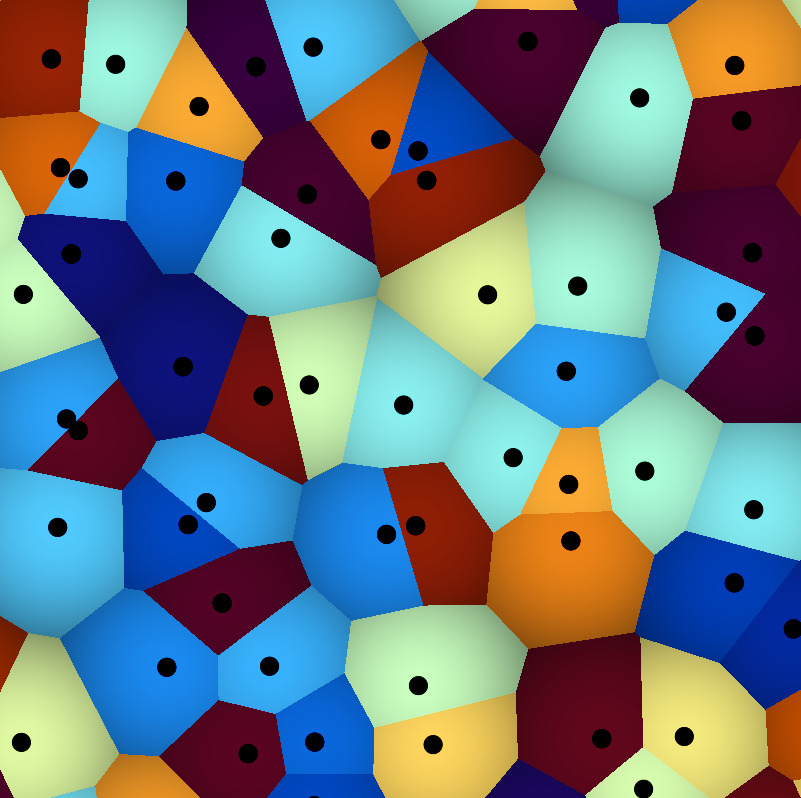
\includegraphics[width=0.32\textwidth]{figures/3-fastsim/voronoi.jpg}
  
\includegraphics[width=0.32\textwidth]{figures/3-fastsim/voronoi_apollonian.jpg}
  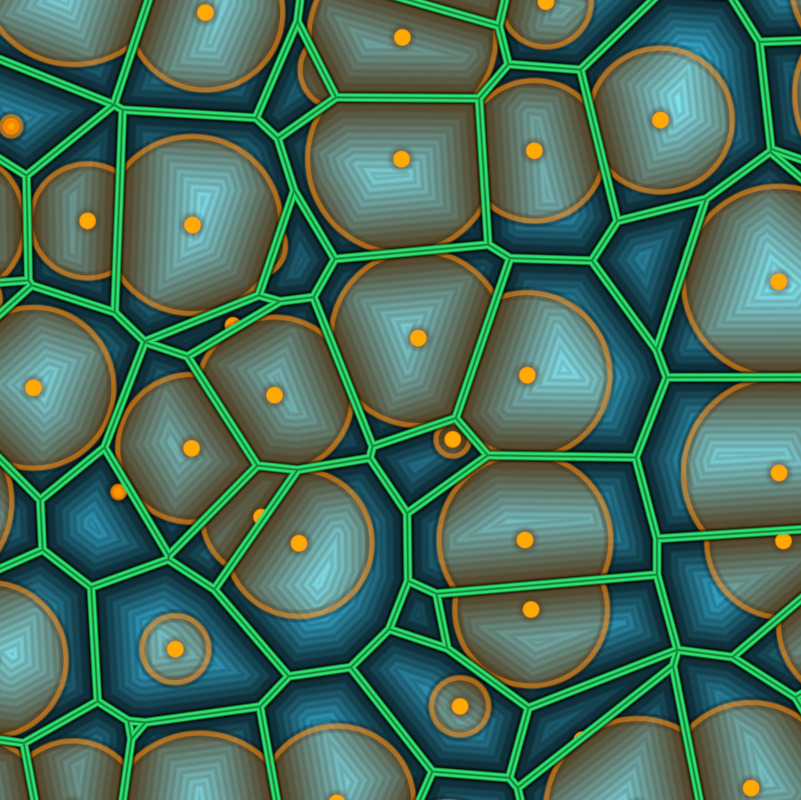
\includegraphics[width=0.32\textwidth]{figures/3-fastsim/voronoi_radical.jpg}
  \caption{Bidimensional illustrations of a Voronoi decomposition using three types of algorithm: (i) for equally sized circles using the equation~\ref{eq:voronoi_partition} (\url{www.shadertoy.com/view/MslGD8}) (ii) for unequally sized circles using the Apollonian Voronoi decomposition condition~\ref{eq:r_voronoi_apollonian} (\url{www.shadertoy.com/view/4sd3D7}) and (iii) another algorithm for unequally sized circles using the radical Voronoi condition~\ref{eq:r_voronoi_radical} (\url{www.shadertoy.com/view/4tV3z3}). Note that the second picture shows the curved boundaries between the Voronoi cells, while the switch to the radical Voronoi decomposition gives straight line boundaries.}\label{fgr:voronoi_illustration}
\end{figure}

This regular Voronoi tessellation can only be used to separate the space for equally sized atoms because it sets the boundaries at equidistance of all the surrounding atoms, as we can see on the Figure~\ref{fgr:voronoi_illustration}. For unequally sized atoms, this type of definition could be undesired since the boundary can be closer to the surface of an atom than of another. The initial thought behind using a Voronoi decomposition is based on delimiting a region for each atom that is closer to this atom than any other one. The ambiguity of this definition relies on the definition of ``closeness''. In this regular Voronoi decomposition, we define the closeness using the distance between the center of mass of the different atoms, which is problematic for unequally distributed radii.

\subsubsection{Unequal radii}

The last definition of the Voronoi decomposition works only for equal-sized atoms because the closest region to an atom is also the closest to its center of mass, which does not apply to the complex atomic structures of nanoporous frameworks. To model the atomic radii $r_1,\ldots,r_n$ of the points $\vect{x}_1,\ldots,\vect{x}_n$ in the same box $B$, we can implement a so-called Apollonian Voronoi diagram.\autocite{voronoi_apollonian} For every $k\in\{1,\ldots,n\}$, the new subspaces $A_{k}$ are defined as follows:

\begin{equation}\label{eq:r_voronoi_apollonian}
  A_{k} = \left\{\vect{x} \in B\ \ |\ \ \forall\ l\neq k,\ {\lVert \vect{x}-\vect{x}_k \rVert}_2 - r_k \leq {\lVert \vect{x}-\vect{x}_l \rVert}_2 - r_l \right\}
\end{equation}

This new definition of the Voronoi diagram has been built on the intuitive property that stipulates that the subspace is the set of points closest to the surface of the sphere around the associated atom. It deals therefore with an unequal distribution of atomic radii, because it is now dependent on the radii. However, as we can see on the Figure~\ref{fgr:voronoi_illustration}, this first implementation has a very convenient definition, but the edges of the subspaces are curved, which makes it harder to use computationally. 

For this reason a less intuitive implementation is more commonly used instead, which is called the radical Voronoi tessellation or power diagram or Laguerre-Voronoi diagram.\autocite{aurenhammer_1987} As we can see on the Figure~\ref{fgr:voronoi_illustration}, the subspaces obtained using this method are now convex polygons with straight edges instead of curved ones. The condition is way less intuitive because the condition does not rely on a simple definition. The subspaces $V_k$ are now defined by the following condition:

\begin{equation}\label{eq:r_voronoi_radical}
    V_{k} = \left\{\vect{x} \in B\ \ |\ \ \forall\ l\neq k,\ {\lVert \vect{x}-\vect{x}_k \rVert}_2^2 - r_k^2 \leq {\lVert \vect{x}-\vect{x}_l \rVert}_2^2 - r_l^2 \right\}
  \end{equation}

In addition to the polyhedral form of the Voronoi cells, this new implementation presents interesting properties for porosity calculations in a framework of unequal spheres like in MOFs of zeolites.\autocite{voronoi_radical} First, the boundary between two overlapping spheres corresponds simply to the intersection place between the spheres. Then, the boundary between non-overlapping spheres is always in the void space between the spheres. This can be simply proven by taking a point $\vect{x}$ in $V_{k}$ and outside the sphere, we have ${\lVert \vect{x}-\vect{x}_k \rVert}_2 \geq r_k$, which implies $\forall\ l\neq k$, ${\lVert \vect{x}-\vect{x}_k \rVert}_2 \geq r_k$. The point $\vect{x}$ is therefore also not overlapping with any other atom, which means it is in the void space of the framework. 

If we now consider a point $\vect{v}$ on a boundary between $p$ Voronoi cells $\left\{V_{i_1},\ldots,V_{i_p}\right\}$, this point would verify all the conditions ${\lVert \vect{x}-\vect{x}_{i_1} \rVert}_2^2 - r_{i_1}^2 = \cdots = {\lVert \vect{x}-\vect{x}_{i_p} \rVert}_2^2 - r_{i_p}^2 = C$. We can know their minimum distance to the center of mass of all nearby atoms to test for possible overlapping. More specifically, in the Zeo++ software,\autocite{Zeo++} the Voronoi diagram is characterized by storing the minimum distance to the closest atoms and the index of the atoms for every vertices and edges (for edges that connect two different periodic images a periodic displacement vector is also stored). This information can be used to speed up the void fraction calculation, by skipping the volume calculations in the non-adsorbable Voronoi cells. It is also a fast way of determining the accessible and non-accessible surface areas and volumes.\autocite{Zeo++} Note that if the probe has a radius $r\e{probe}$, then the sphere radii considered are $r_k = r\e{atom}+r\e{probe}$.

\subsection{Implementation in a screening}


The use of the Voronoi decomposition of the pore space of materials for their geometric characterization has been widely employed in computational studies in the last decade,\autocite{Willems_2012}  especially since it was made easily available as part of the Zeo++ software package.\autocite{Pinheiro2013} Its use was extended recently to implement a novel sampling scheme, in a study  that introduces the ML-assisted screening of nanoporous materials for xenon/krypton separation. In this article, Simon et al.\autocite{Simon_2015} relied on a Voronoi tessellation of the nanoporous materials and assigned the potential adsorption sites (i.e., the sampling points) at the nodes of this decomposition. The Voronoi tessellation identifies the vertices of polyhedra that correspond to the closest regions of each atom of the structure. These vertices (or \emph{Voronoi nodes}) are the points equidistant to at least four atoms of the structure, and they can be associated with adsorption sites since they are positioned near the center of the pores. 

The definition of accessibility defined by the Zeo++ software was used in a screening to find the best materials for Xe/Kr separation.\autocite{Simon_2015} The interaction energies of xenon were calculated only on the accessible nodes as schemed on the Figure~\ref{fgr:simon_voro}. The average of the energies at the accessible Voronoi nodes gives an approximation of the adsorption enthalpy. However, this sampling assumes that the nodes are close to the real, most favorable, adsorption sites. Or to put it differently, the adsorption sites need to be at the center of the pores, which is only true for structures with pore sizes close to adsorbate size. This newly defined adsorption energy descriptor was found to be one of the most influential descriptors for the ML model developed to predict the ambient-pressure selectivity. 

\begin{figure}[ht]
  \centering
  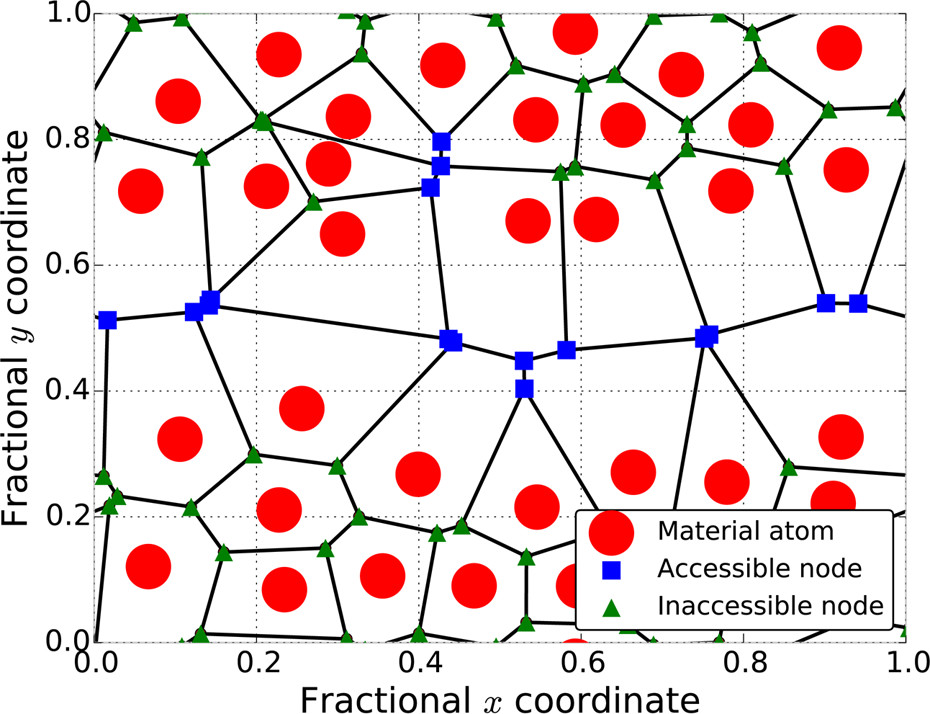
\includegraphics[width=0.5\textwidth]{figures/3-fastsim/Simon_voronoi.jpeg}
  \caption{Voronoi network model of void space (2D caricature). The unit cell of a toy material is shown. Red circles represent atoms of the material; accessible and inaccessible Voronoi nodes are blue squares and green triangles, respectively. The black lines are the edges in the periodic Voronoi graph that model the void space. Reprinted with permission from Ref.~\cite{Simon_2015}. Copyright 2015 American Chemical Society.}\label{fgr:simon_voro}
\end{figure}

Starting from the initial idea of Voronoi sampling, we want to question the relevance of using a direct average of the interaction energies instead of a Boltzmann averaging in describing the adsorption enthalpy. To better understand the strengths and weaknesses of this methodology, we compared different ways of approximating adsorption enthalpies using the Voronoi sampling with more accurate infinite dilution and ambient-pressure xenon adsorption enthalpies using Widom insertions and GCMC for a 20:80 Xe/Kr mixture at \SI{1}{\atm} and \SI{298}{\kelvin}.

\subsection{Comparative study of the Voronoi sampling}

We introduced in the previous chapter, the definition of the xenon adsorption enthalpy at infinite dilution (Widom insertion section~\ref{sct:widom}) and at ambient pressure (GCMC sections~\ref{sct:GCMC} and~\ref{sct:thermo}). These methods can be considered accurate methods to calculate the adsorption enthalpy which has been proven to be strongly correlated to the logarithm of the selectivity in our previous study on the thermodynamic exploration of the xenon/krypton separation using a high-throughput screening.

\subsubsection{Introduction of the main concepts}

The Voronoi energy as initially conceptualized by Simon et al.\ is based on the average of the xenon interaction energies at the accessible Voronoi nodes. But because we will compare to thermodynamic simulations without blocking pockets, we will not consider the accessible Voronoi nodes but the adsorbable ones since it is closer to the simulation we want to approximate. For simplicity, we define the set of the adsorbable Voronoi nodes $A$ as the Voronoi nodes with a negative energy value, we also apply a condition on the minimum distance (about the radius of a xenon \SI{2}{\angstrom}) to reduce the number of points to be calculated. This average on the adsorbable Voronoi nodes $E\e{voro-A}^{Xe}$ can be written:

\begin{equation}
    E\e{voro-A}^{Xe} = \sum_{i \in A} E_i -RT
\end{equation}

Another interesting energy descriptor could simply be the minimum of the interaction energies among the Voronoi nodes $V$ with a minimum distance to the nearest atom is higher than \SI{2}{\angstrom}. This minimum Voronoi energy $E\e{voro-M}^{Xe}$ can be written: 

\begin{equation}
    E\e{voro-M}^{Xe} = \min_{i \in V} E_i
\end{equation}

Finally, to get closer to the definition of the heat of adsorption defined in the previous chapter, we can build an energy descriptor using a Boltzmann averaging. This Boltzmann average of the xenon interaction energies at the Voronoi nodes $V$ written $E\e{voro-B}^{Xe}$ can be expressed as follows:

\begin{equation}
    E\e{voro-B}^{Xe} = \dfrac{\sum\limits_{i \in V} E_i e^{-\beta E_i}}{\sum\limits_{i \in V} e^{-\beta E_i}} -RT
\end{equation}
Note that the $-RT$ term is to make the expression comparable to the one of adsorption enthalpy. 

We can intuitively say that the Boltzmann averaging being closer to the definition of the adsorption enthalpy it would be a better candidate as an energy descriptor, hence improving the screening methodology. To test these different methodologies, we will now compare the different energy descriptors to more accurate evaluation of the adsorption heat. 

\subsubsection{Low-pressure comparison}

The Widom insertion is typically used to calculate the infinite dilution adsorption properties such as the adsorption enthalpy, the Henry constant and the selectivity. The evaluation of the interaction energies of xenon at the different Voronoi nodes correspond to a low-pressure averaging and is more comparable to a Widom insertion method. It is, however, biased by the inhomogeneous sampling of the space, which can explain some discrepancies we could observe.

Note that in this chapter we will mainly use the standard pore size definition we find in the literature that is based on the atom radii defined by the Cambridge Crystallographic Data Centre (CCDC). This pore size will only serve a labeling purpose and will help us classify the structures according to their relative size. It has qualitative role mainly, which justifies the fact that we are not using a much more accurate definition based on the forcefield like in the previous chapter. 

As we can see on the Figure~\ref{fgr:compa_voro_0}, the average of the energies is not performing very well and is clearly less correlated to the adsorption enthalpy than the minimum interaction energy or the Boltzmann average of the interaction energies. This is because in a normal average, the high-energy values have a much higher weight than in a Boltzmann average, which makes the average much more important than expected. The Voronoi average descriptor $E\e{voro-A}^{Xe}$ is always higher than the infinite dilution adsorption enthalpy $\Delta\e{ads} H_{0}\ex{Xe}$. 

\begin{figure}[ht]
  \centering
    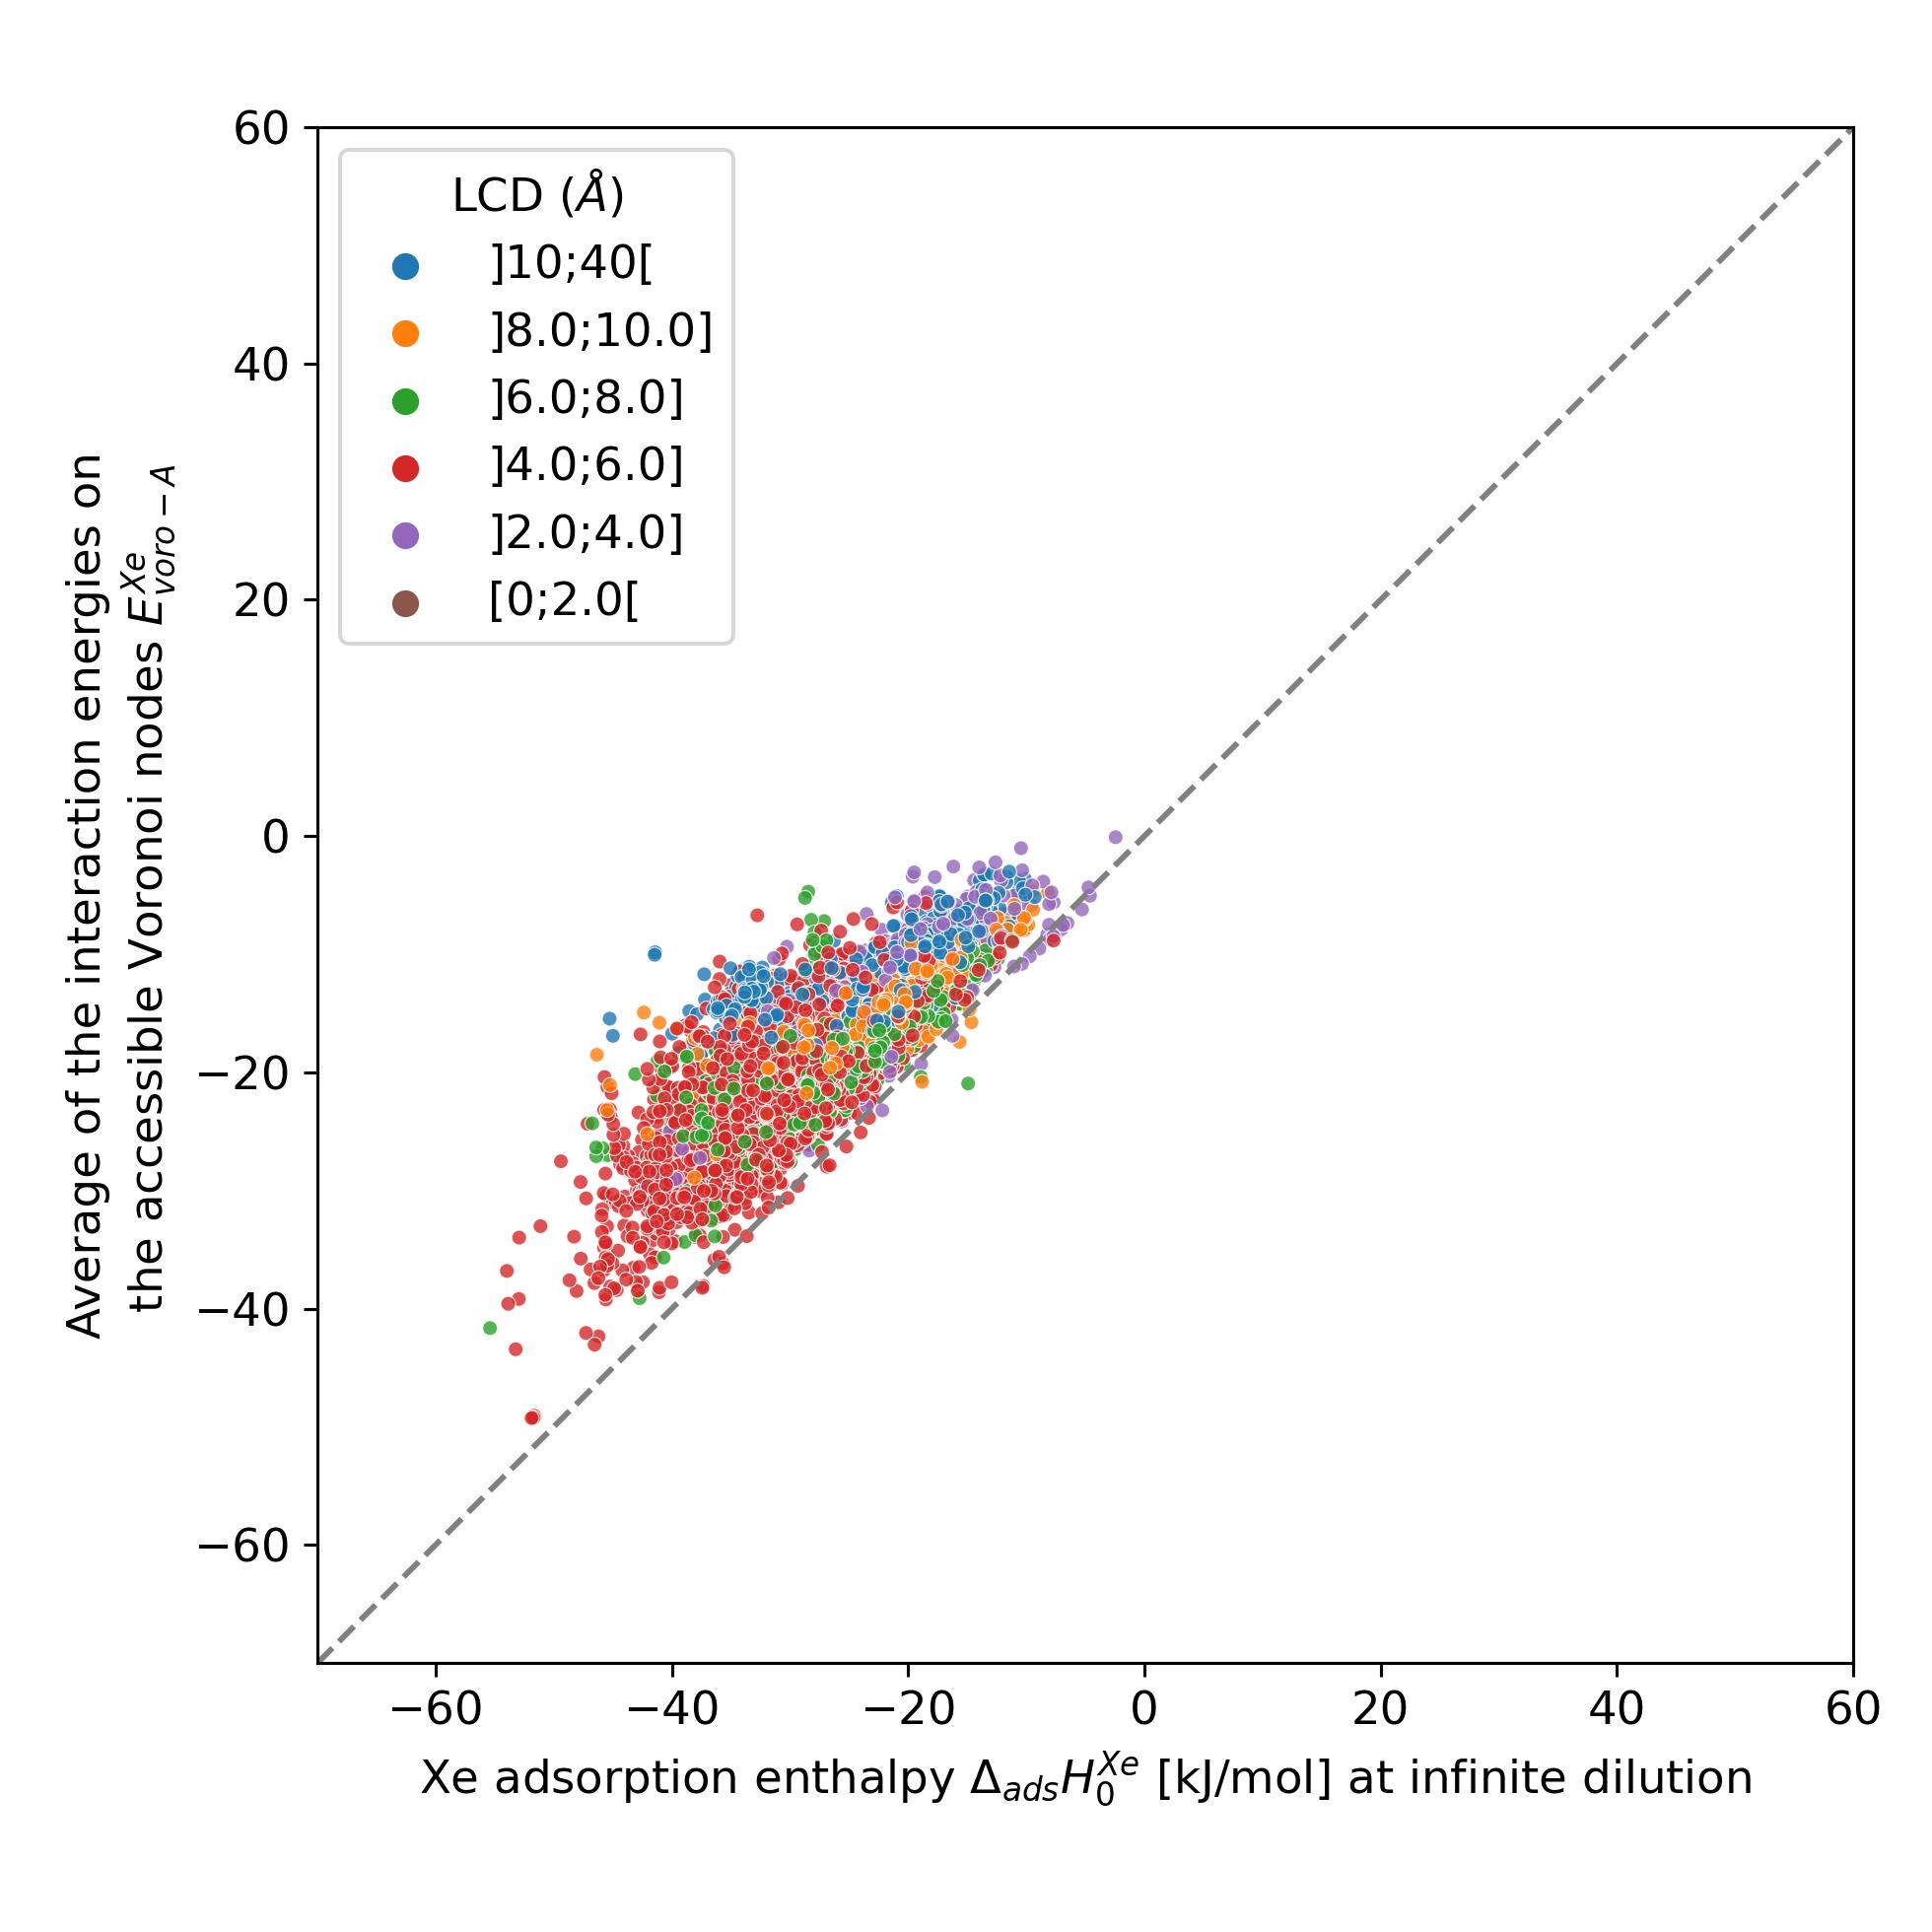
\includegraphics[width=0.32\textwidth]{figures/3-fastsim/H_Xe_0_vs_E_voro_A_overview.jpg}
    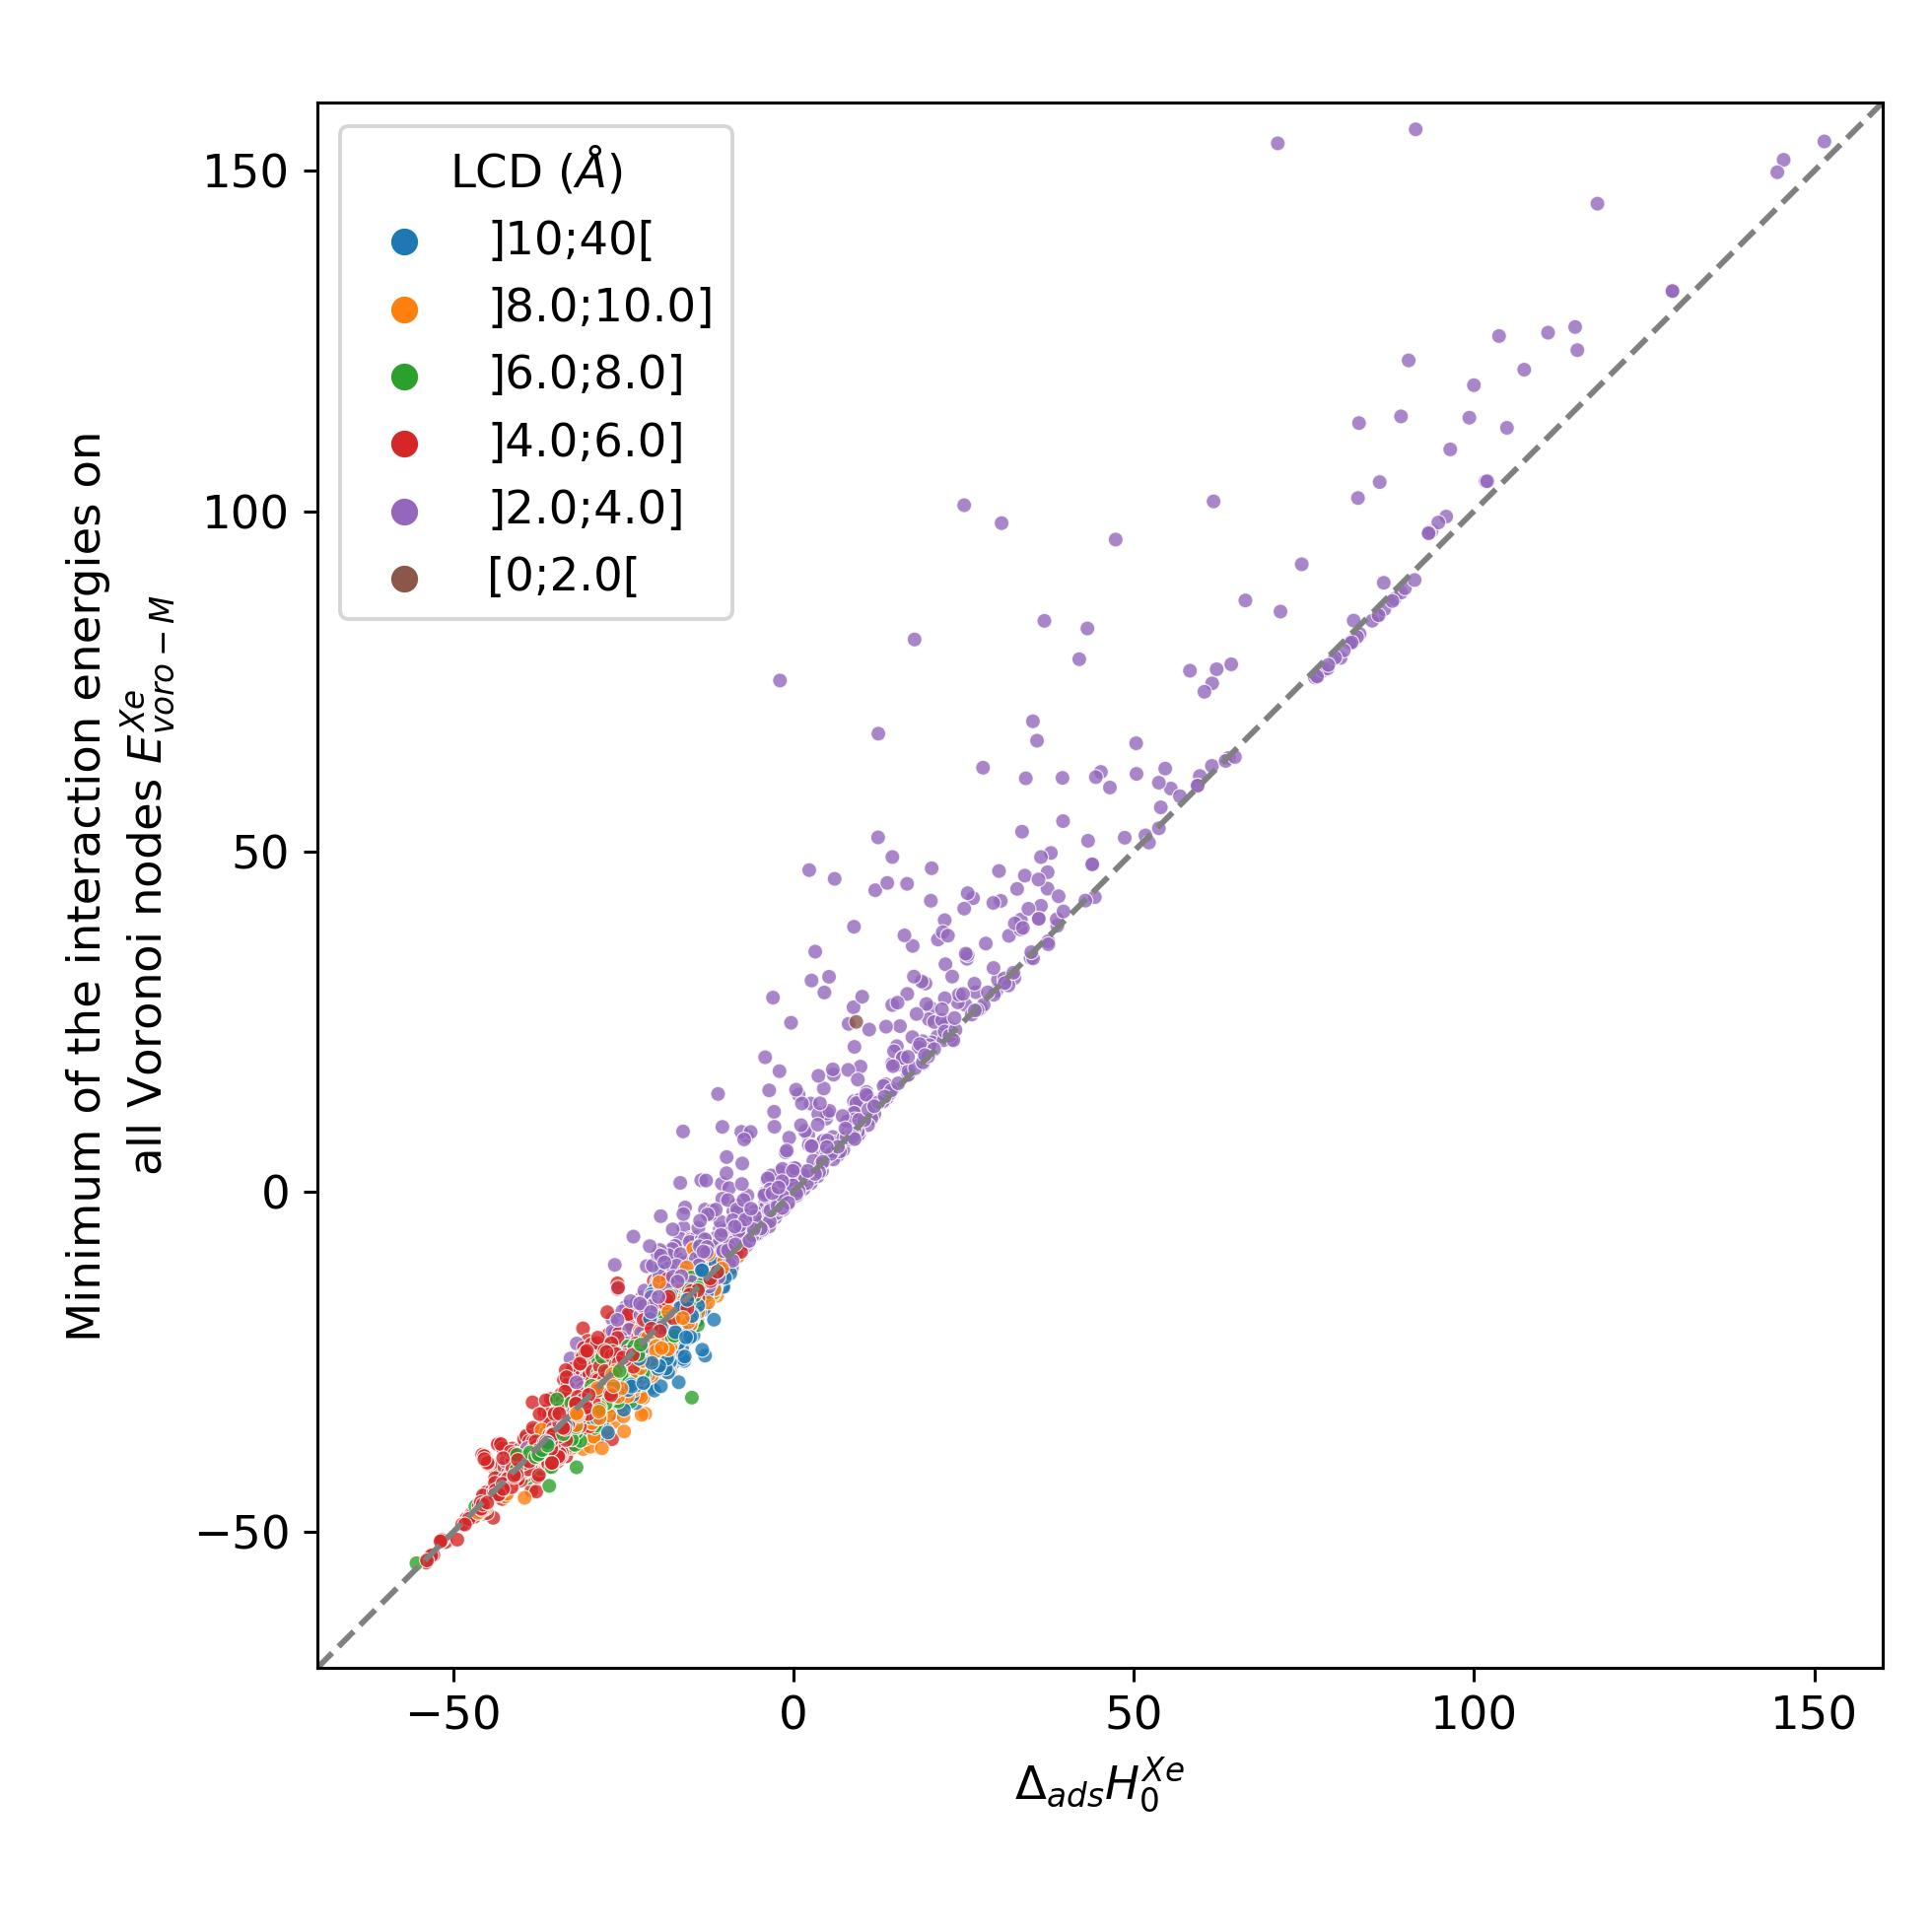
\includegraphics[width=0.32\textwidth]{figures/3-fastsim/H_Xe_0_vs_E_voro_M_overview.jpg}
    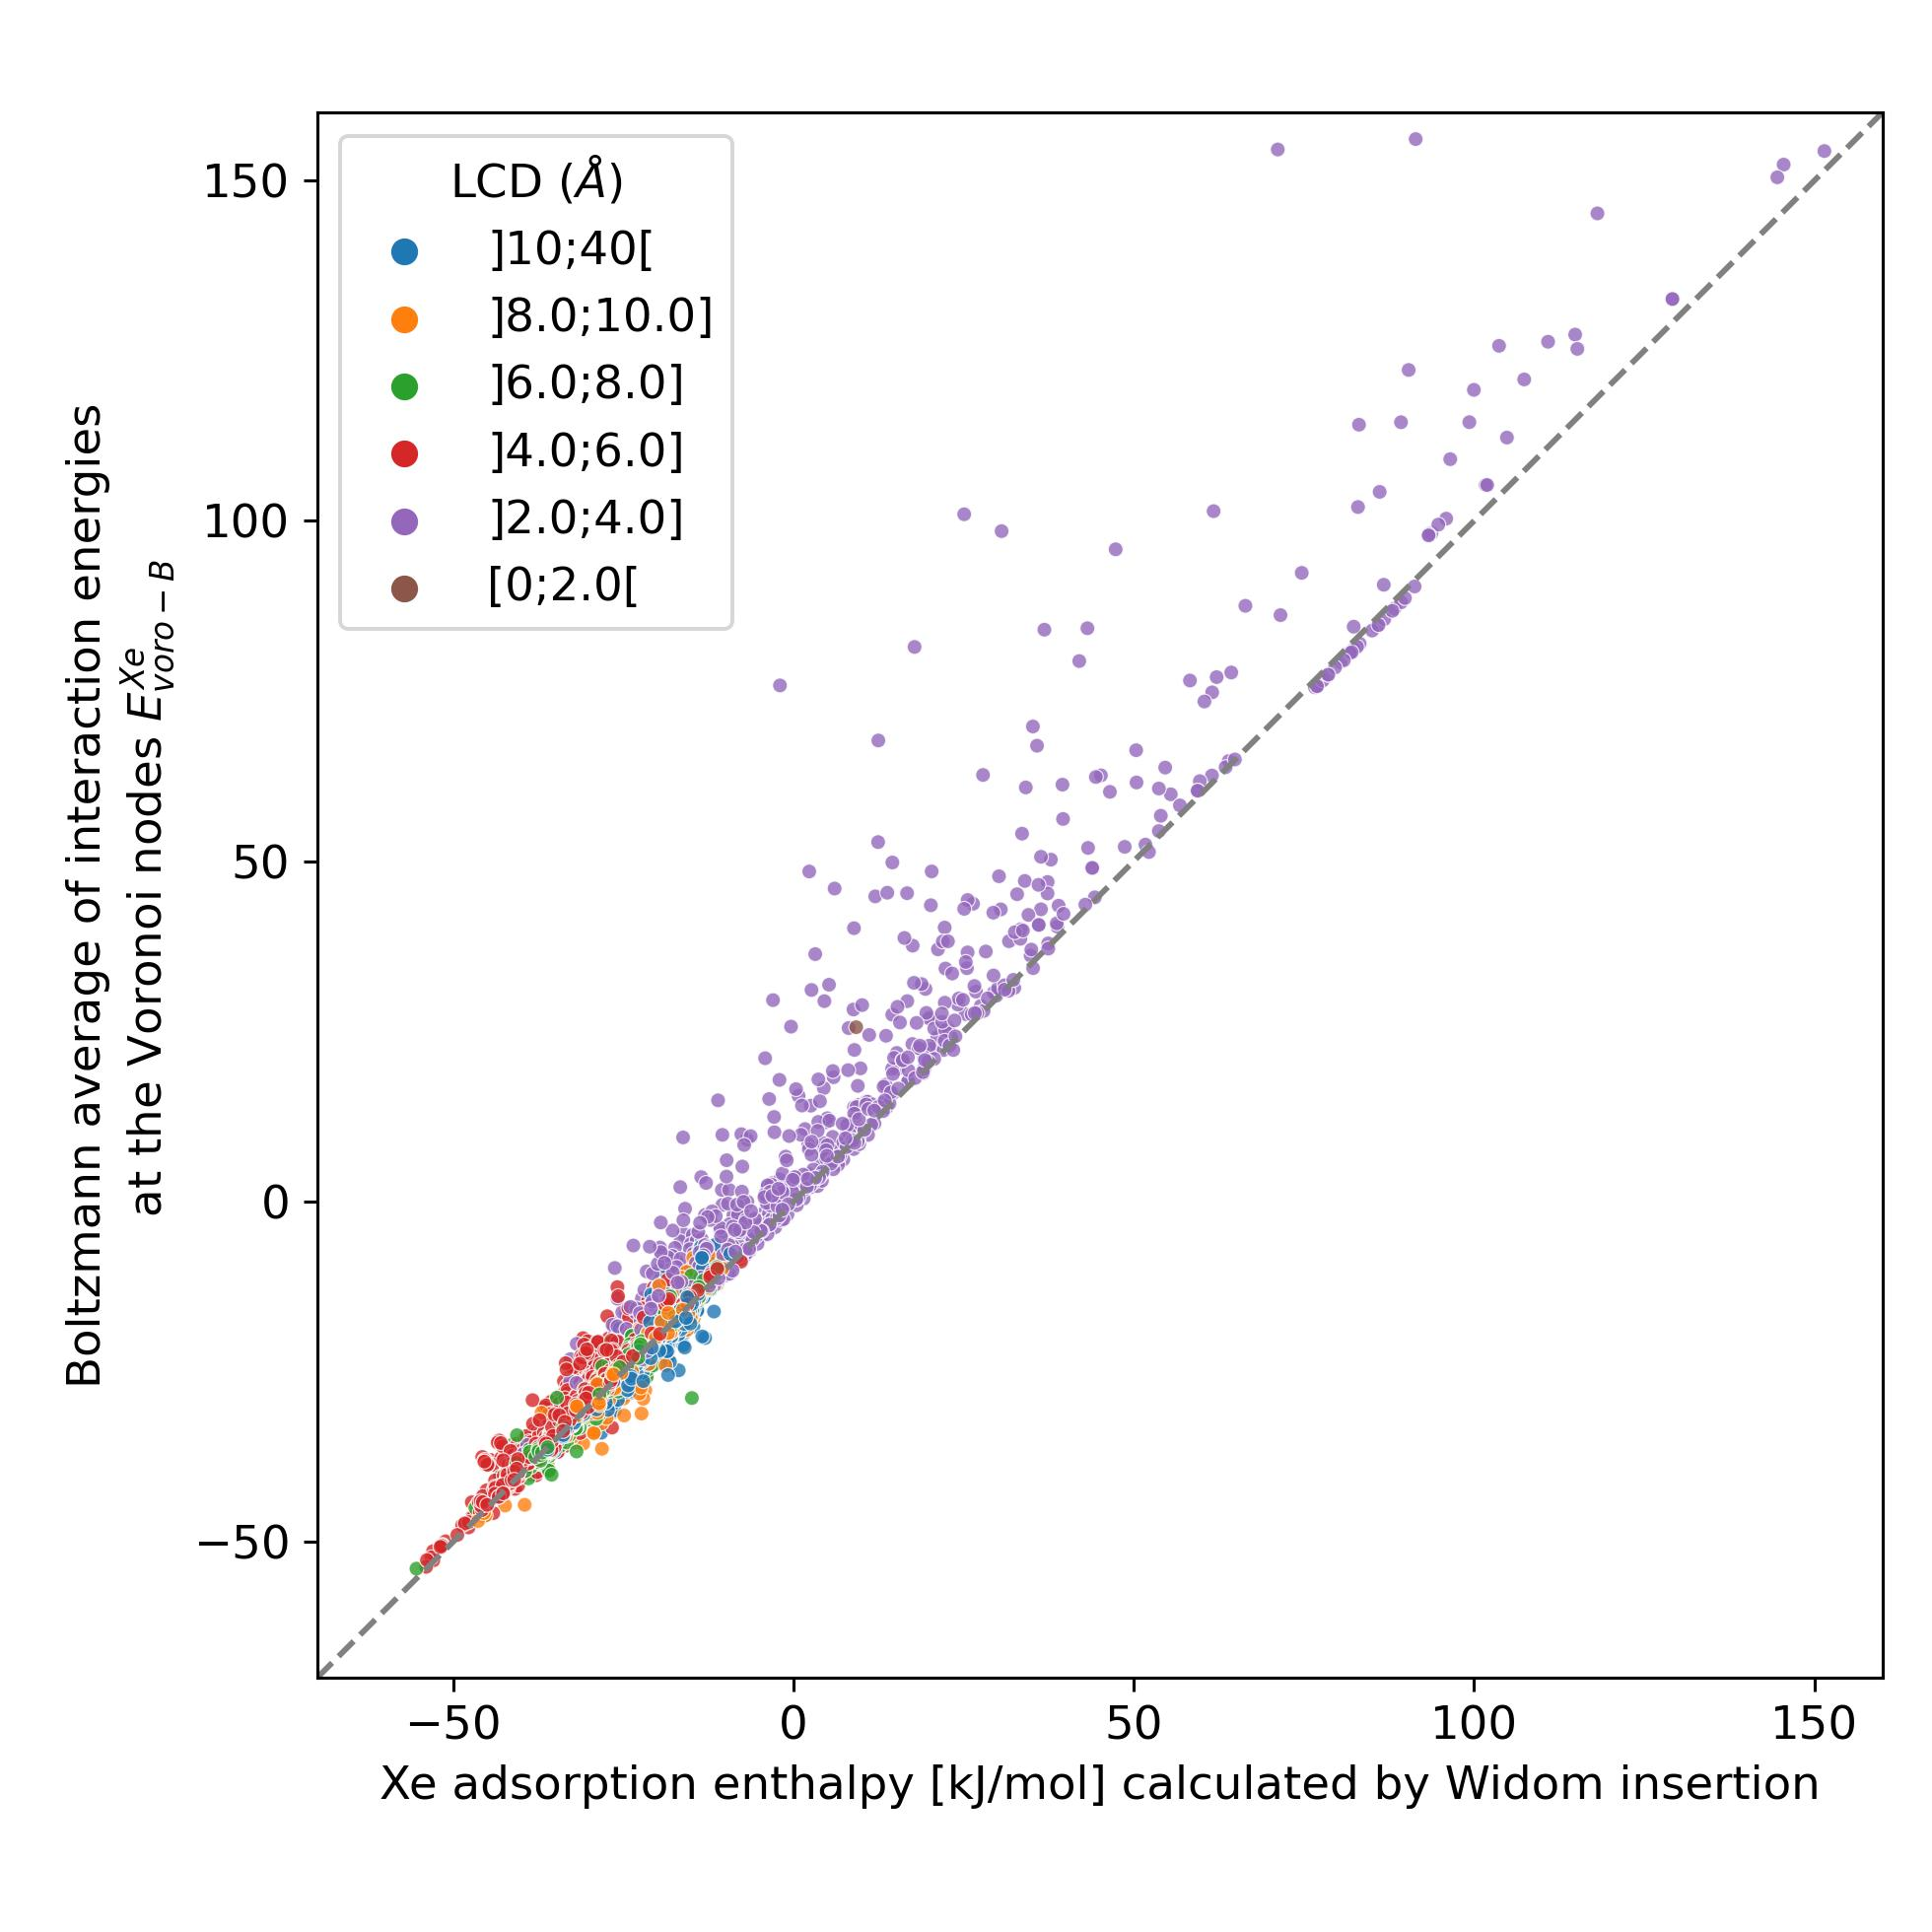
\includegraphics[width=0.32\textwidth]{figures/3-fastsim/H_Xe_0_vs_E_voro_B_overview.jpg}
    \caption{Scatterplots of the energy descriptors $E\e{voro-A}^{Xe}$, $E\e{voro-M}^{Xe}$ and $E\e{voro-B}^{Xe}$ calculated by a Voronoi sampling compared to the enthalpies calculated by a 100k-step Widom insertion simulation of xenon in structures of CoRE MOF 2019. The points are labeled according to the largest cavity diameter (LCD\e{CCDC}) belonging to one of the intervals.}\label{fgr:compa_voro_0}
\end{figure}

The Pearson correlation coefficients corroborate our initial observation. The correlation coefficient between $E\e{voro-A}^{Xe}$ and $\Delta\e{ads} H_{0}\ex{Xe}$ is equal to $0.81$, whereas for the minimum $E\e{voro-M}^{Xe}$ it is $0.95$ and for the Boltzmann average $E\e{voro-B}^{Xe}$ it is $0.97$. For this reason, to evaluate the relevance of a Voronoi energy sampling we should consider a Boltzmann average. As we have shown in the previous chapter, the selectivity is correlated to the difference of adsorption enthalpies of xenon and krypton. Better describing the enthalpy is a first step toward a better description of the selectivity. However, we only looked at the selectivity values at low pressure. What would happen for selectivity at higher pressure?

\begin{figure}[ht]
  \centering
  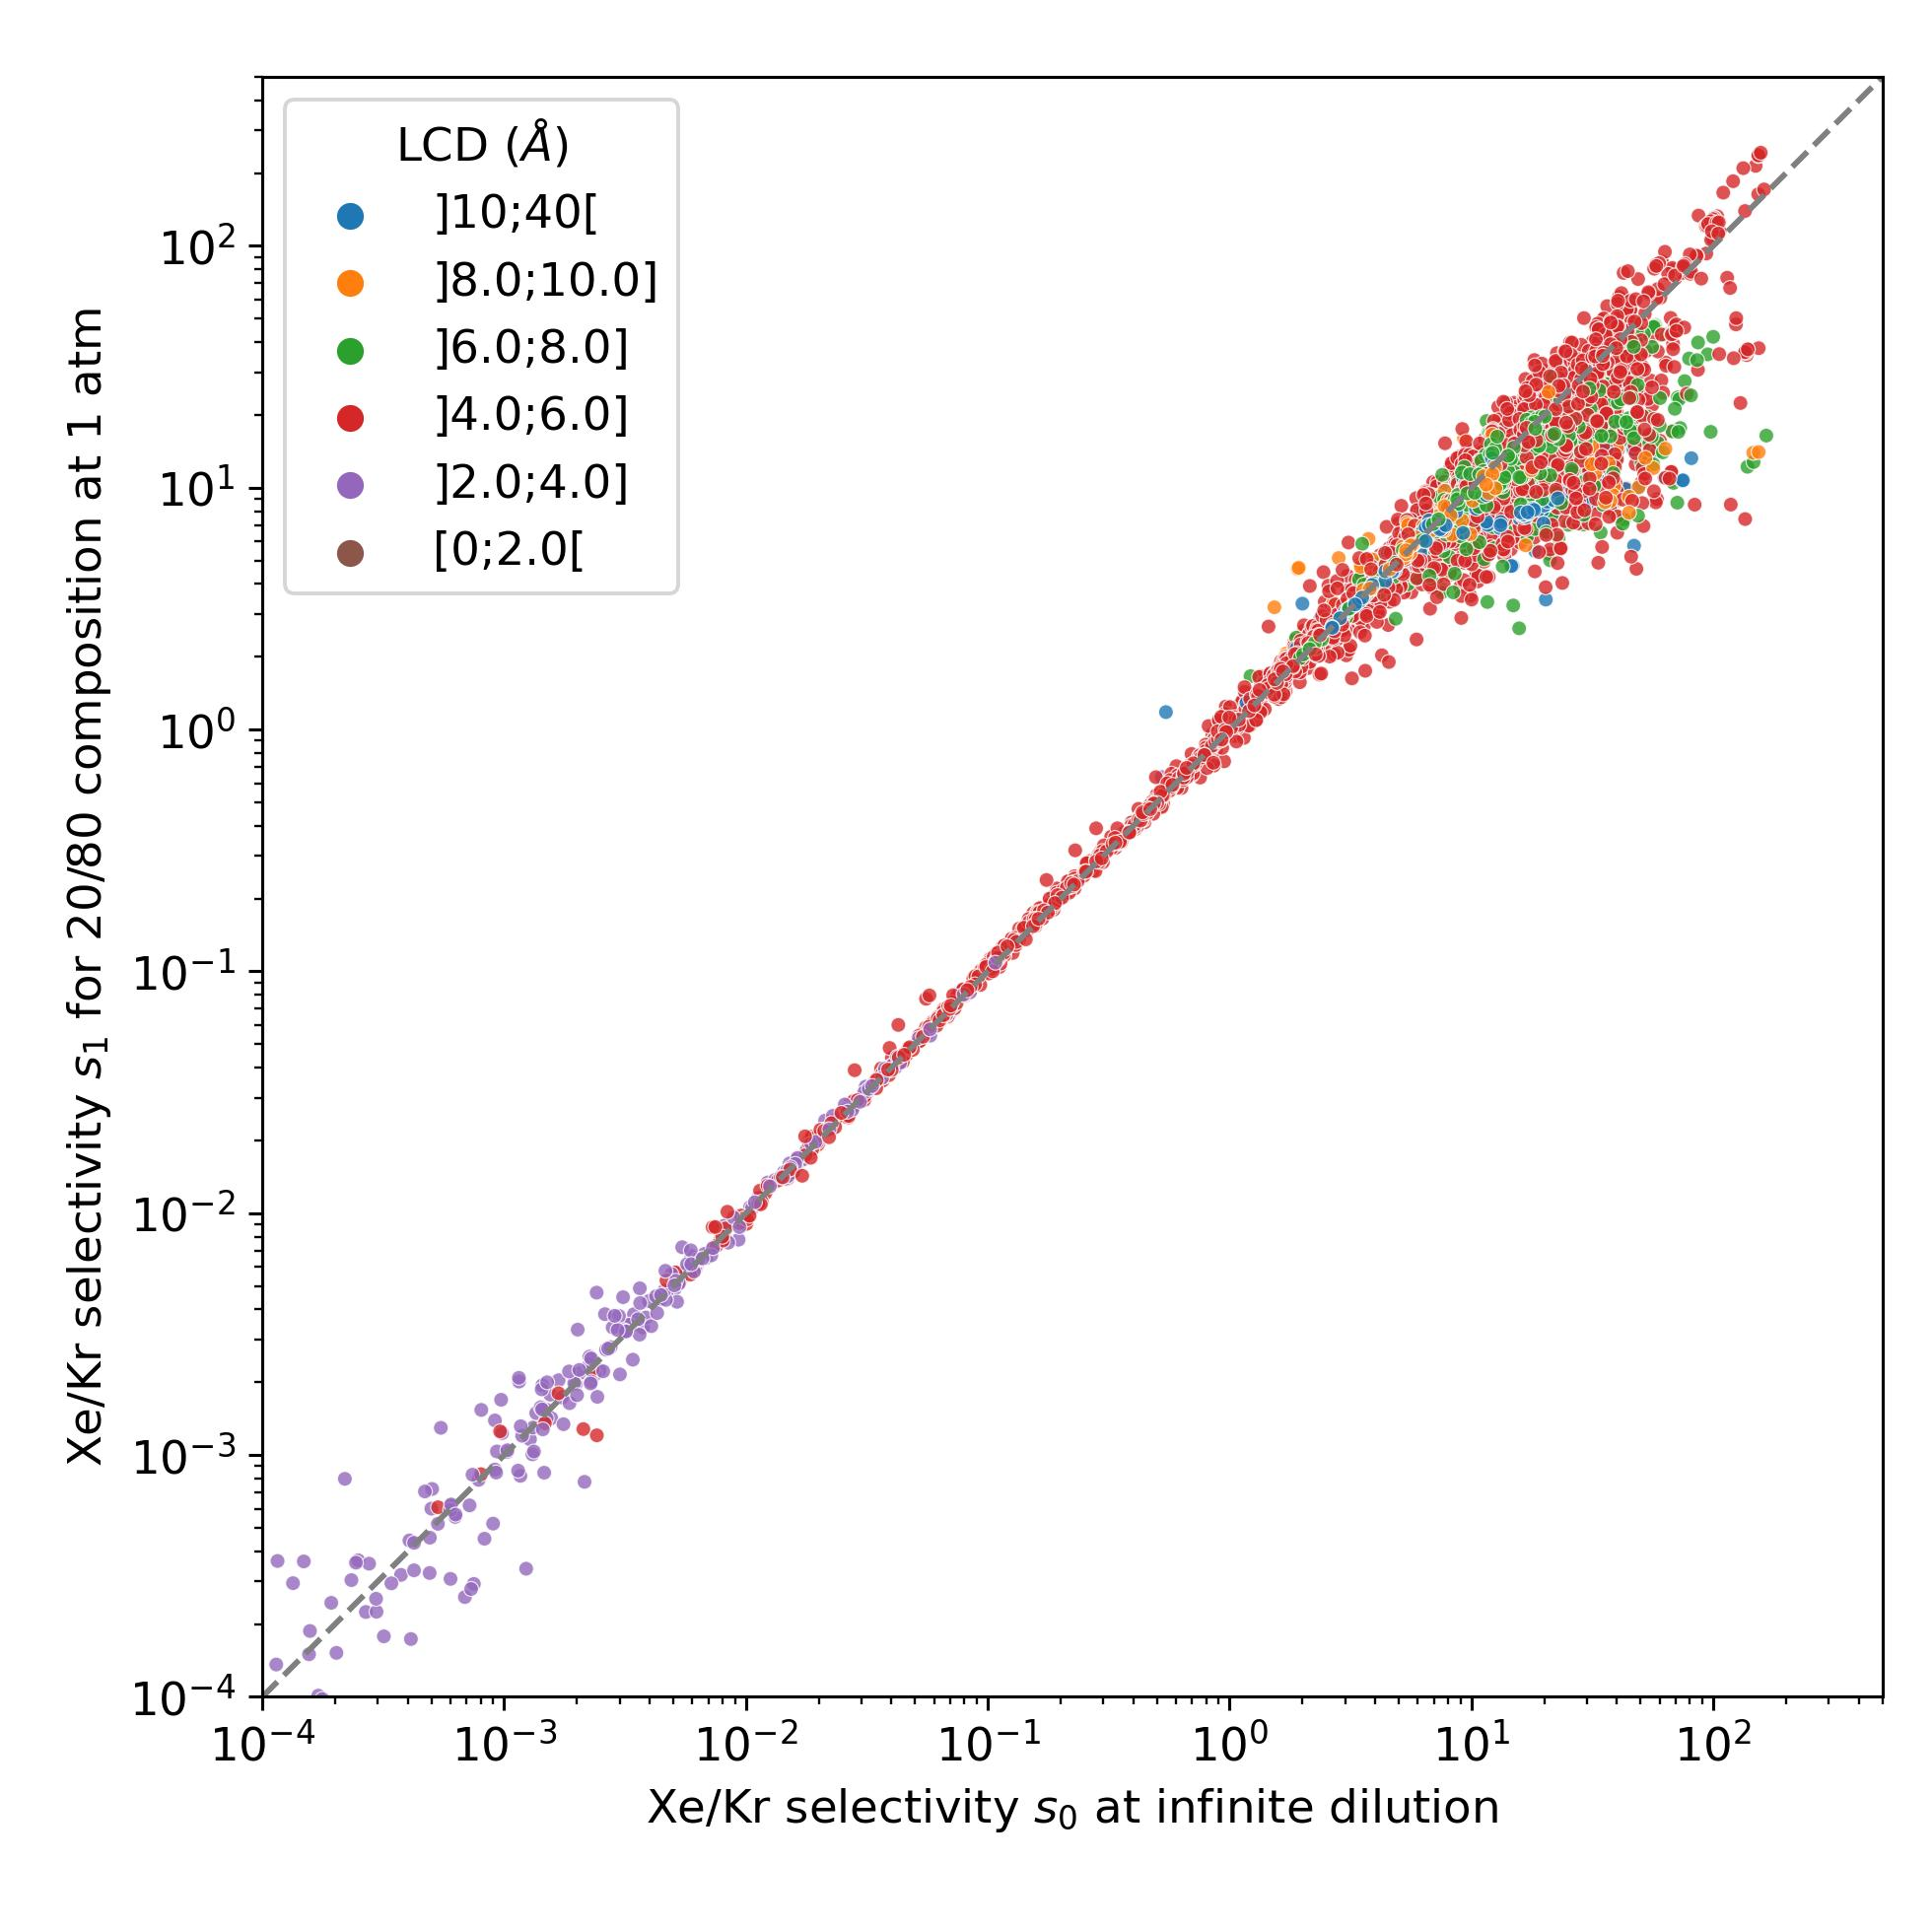
\includegraphics[width=0.45\textwidth]{figures/3-fastsim/s_0_vs_s_2080_overview.jpg}
  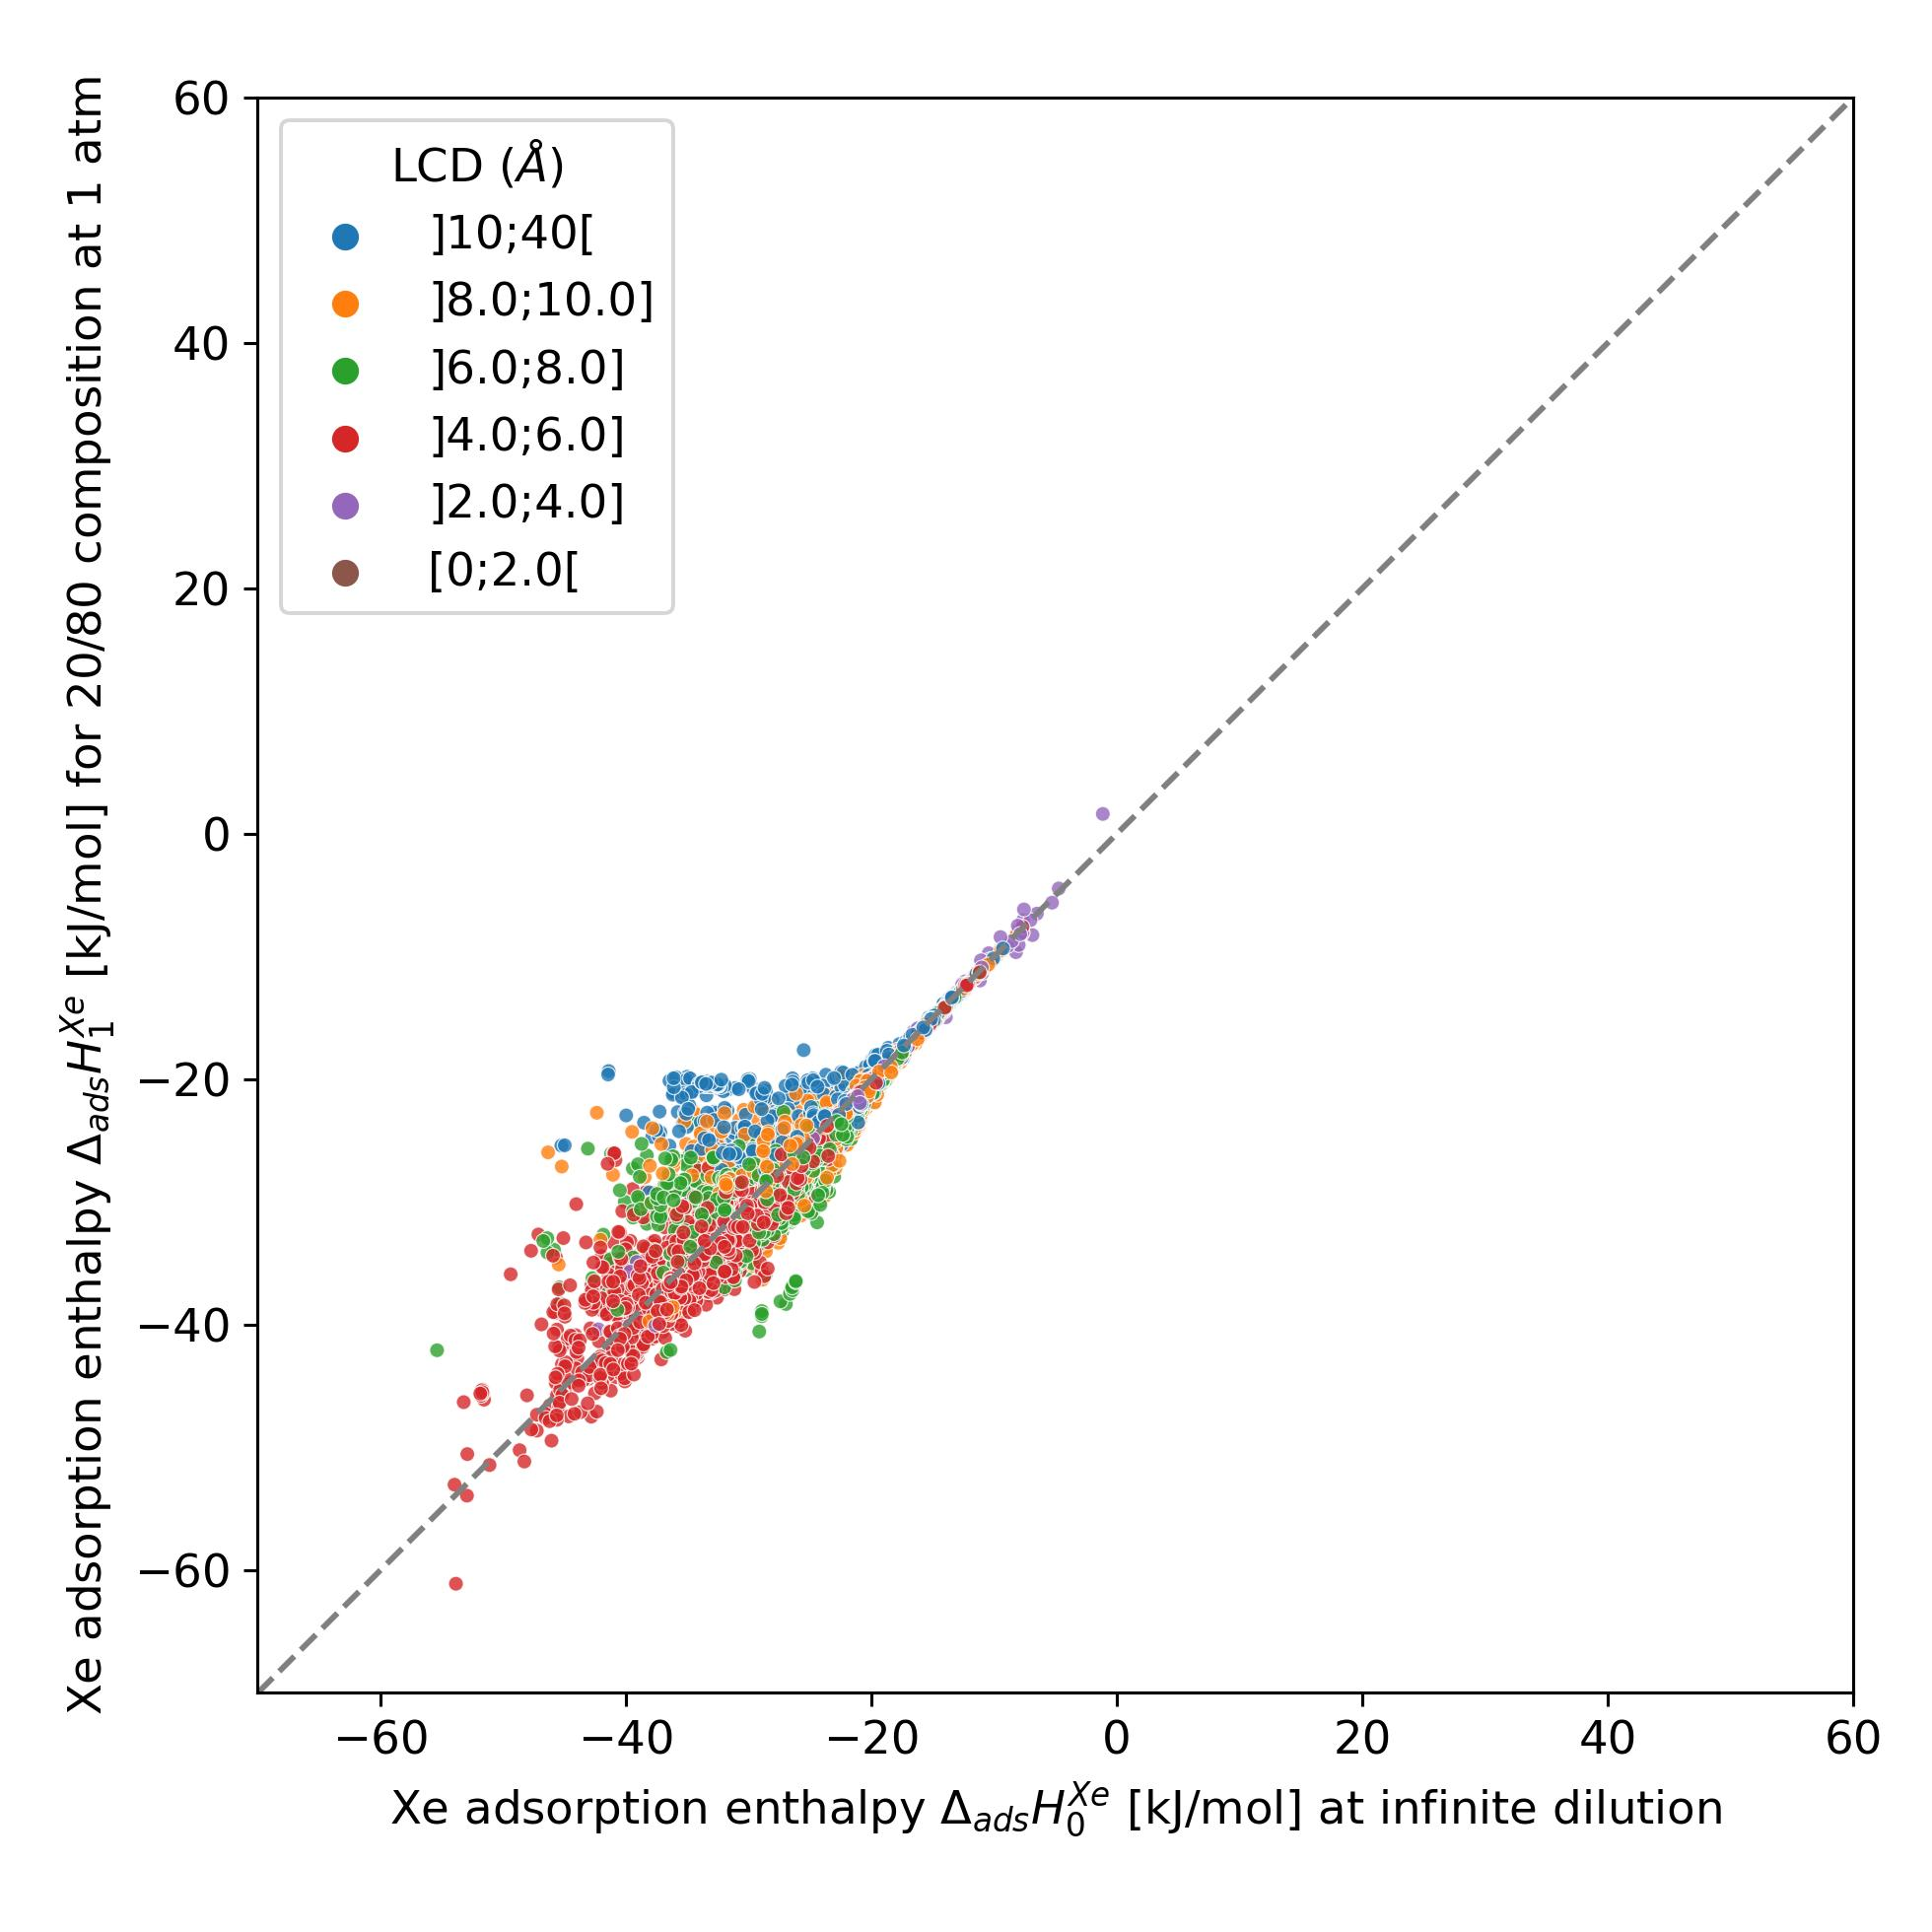
\includegraphics[width=0.45\textwidth]{figures/3-fastsim/H_Xe_0_vs_H_Xe_2080_overview.jpg}
    \caption{Comparison of the ambient-pressure and low-pressure case through two thermodynamic quantities: the Xe/Kr selectivity (left) and the xenon adsorption enthalpy (right). }\label{fgr:compa_pressure}
\end{figure}

On the Figure~\ref{fgr:compa_pressure}, we can see that the selectivity drop between the low-pressure case and the ambient-pressure one also impacts the enthalpy values of xenon. There is a reduction of the xenon affinity as the pressure goes up. Since the study of Simon et al.\ focused on the ambient-pressure selectivity prediction, we want to see if the energy descriptor they developed could, however, be used to describe the adsorption enthalpy at high pressure. 

\subsubsection{Ambient-pressure xenon/krypton separation}

If we look at the Figure~\ref{fgr:compa_voro_2080}, it is not so clear which descriptor is better to describe the enthalpy at ambient pressure. The correlation shown by the different scatterplots seems to be equally poor, and this could justify the use of a regular average rather than a Boltzmann average. The correlation coefficient for the average $E\e{voro-A}^{Xe}$ is now equal to $0.86$, which is equivalent to the one of the minimum $E\e{voro-M}^{Xe}$ and slightly lower than the $0.87$ for the Boltzmann average $E\e{voro-B}^{Xe}$. 

\begin{figure}[ht]
    \centering
      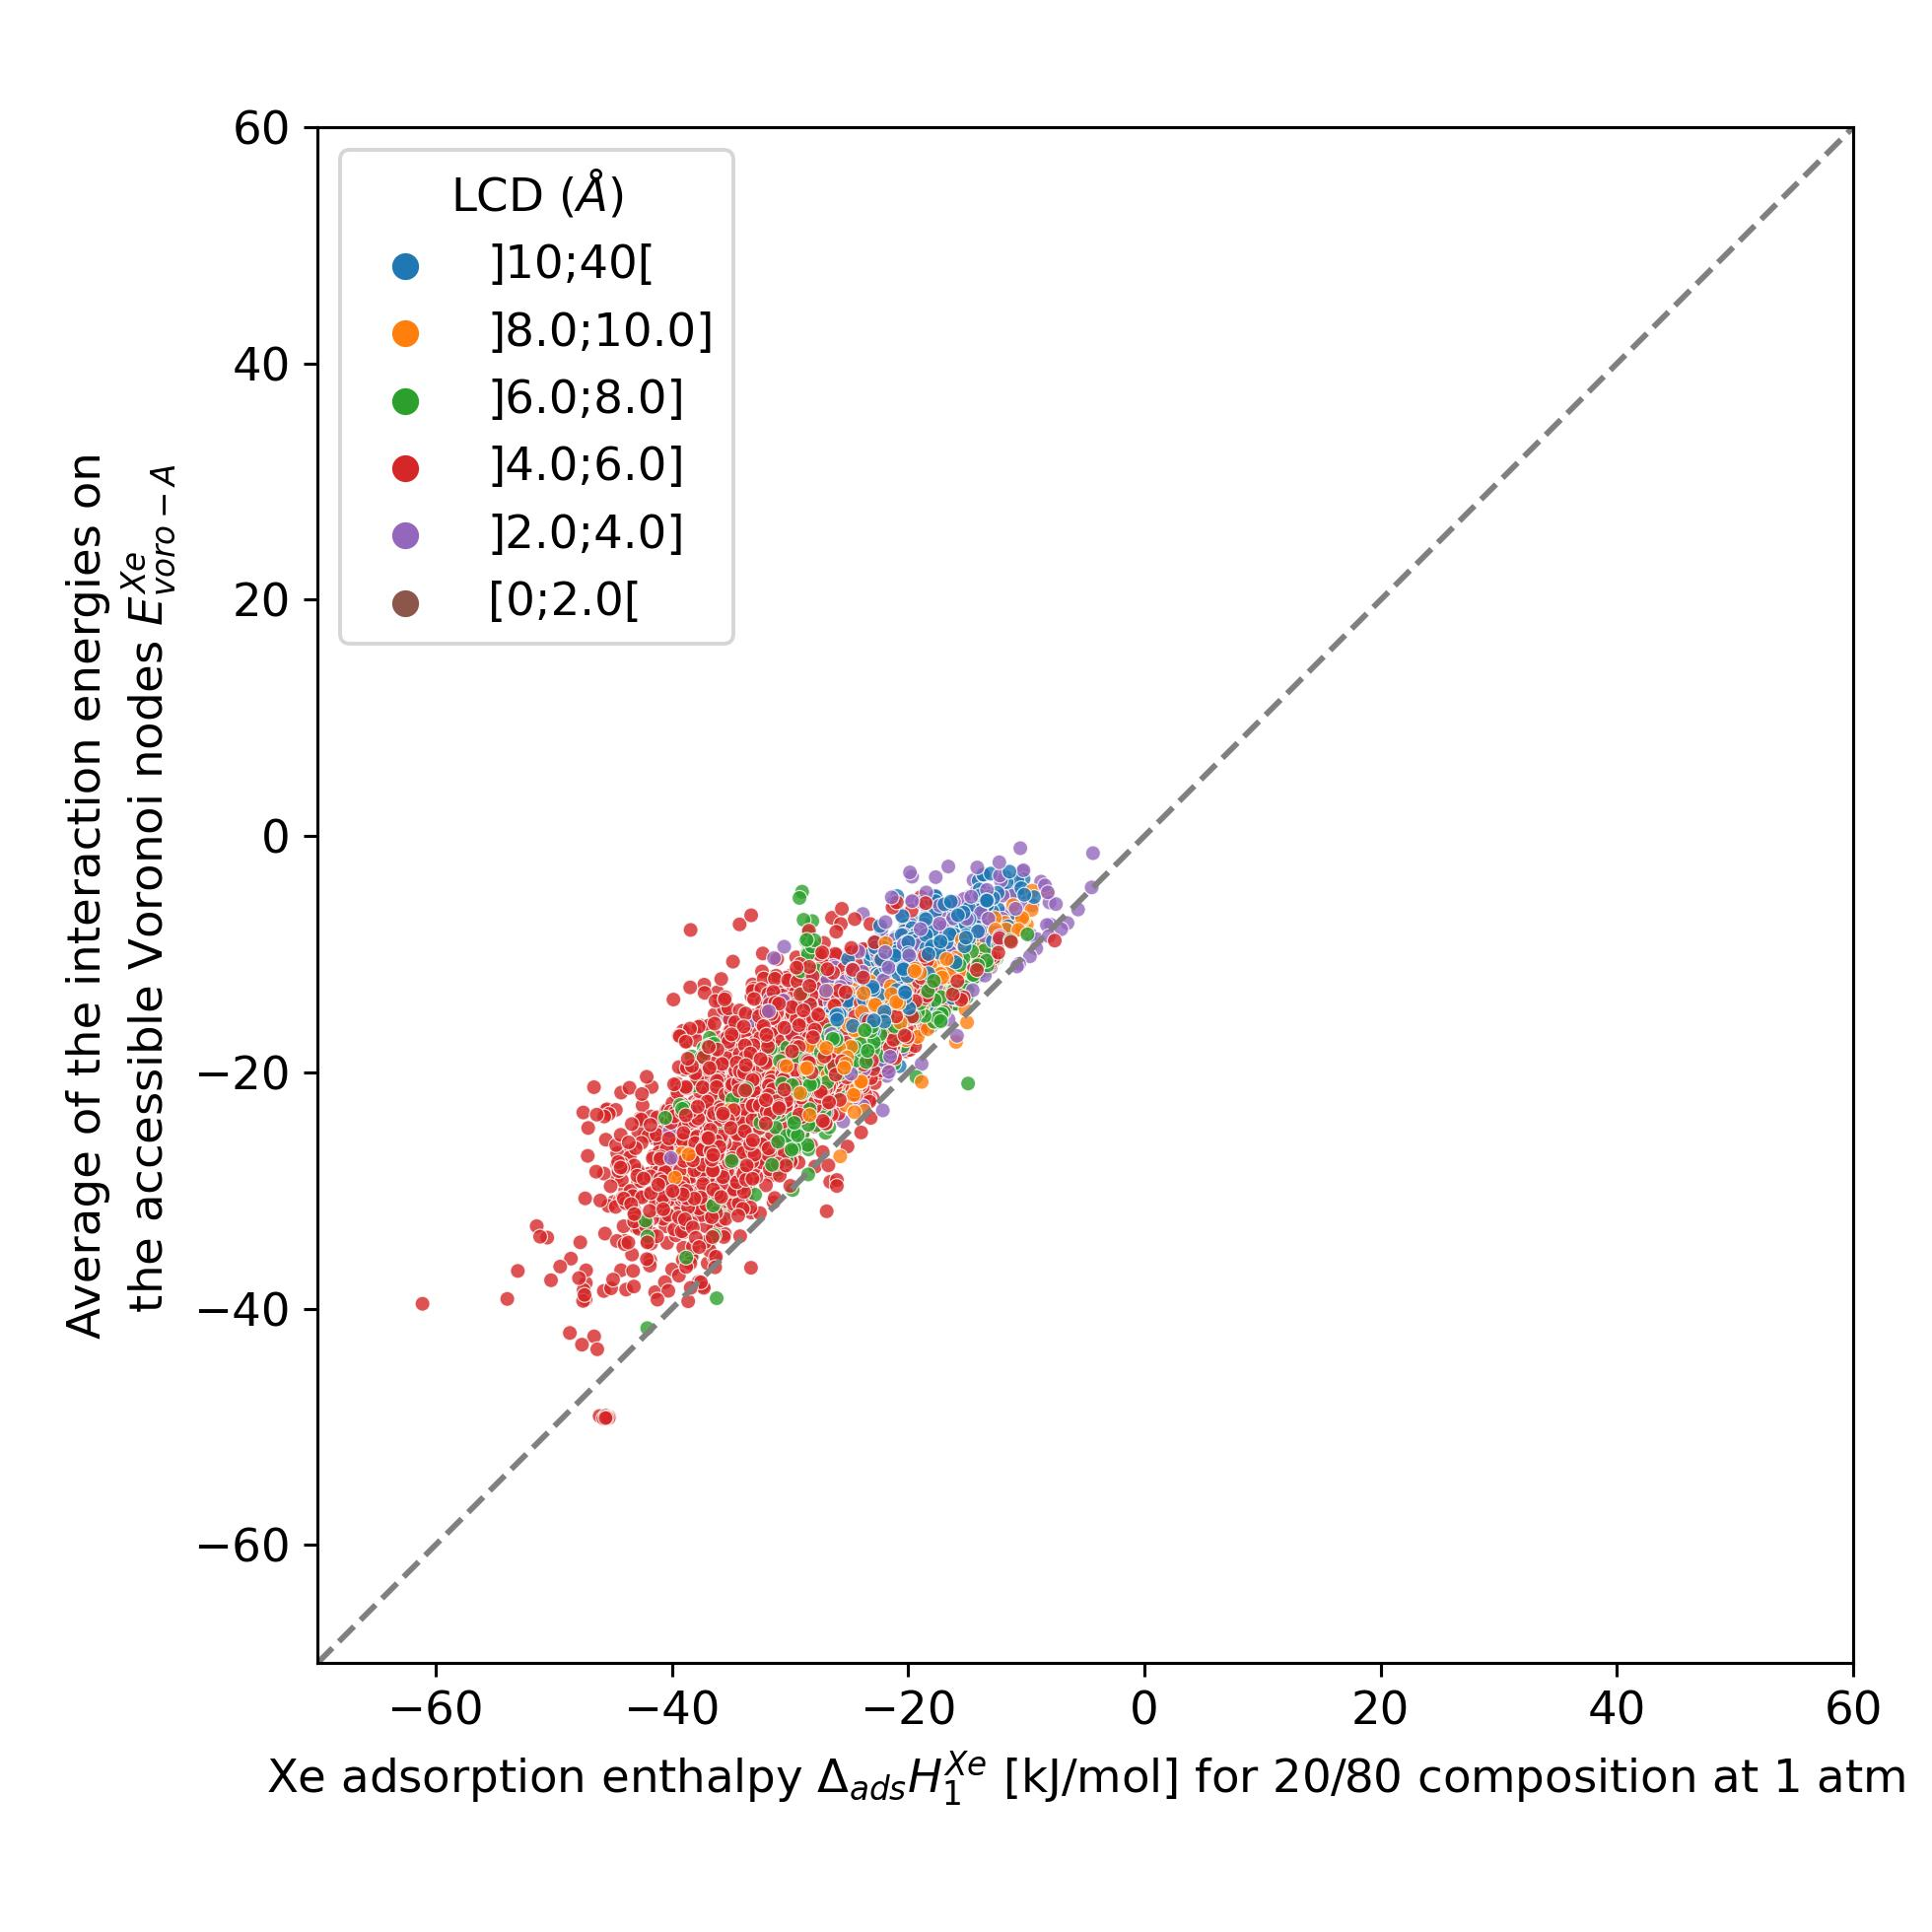
\includegraphics[width=0.32\textwidth]{figures/3-fastsim/H_Xe_2080_vs_E_voro_A_overview.jpg}
      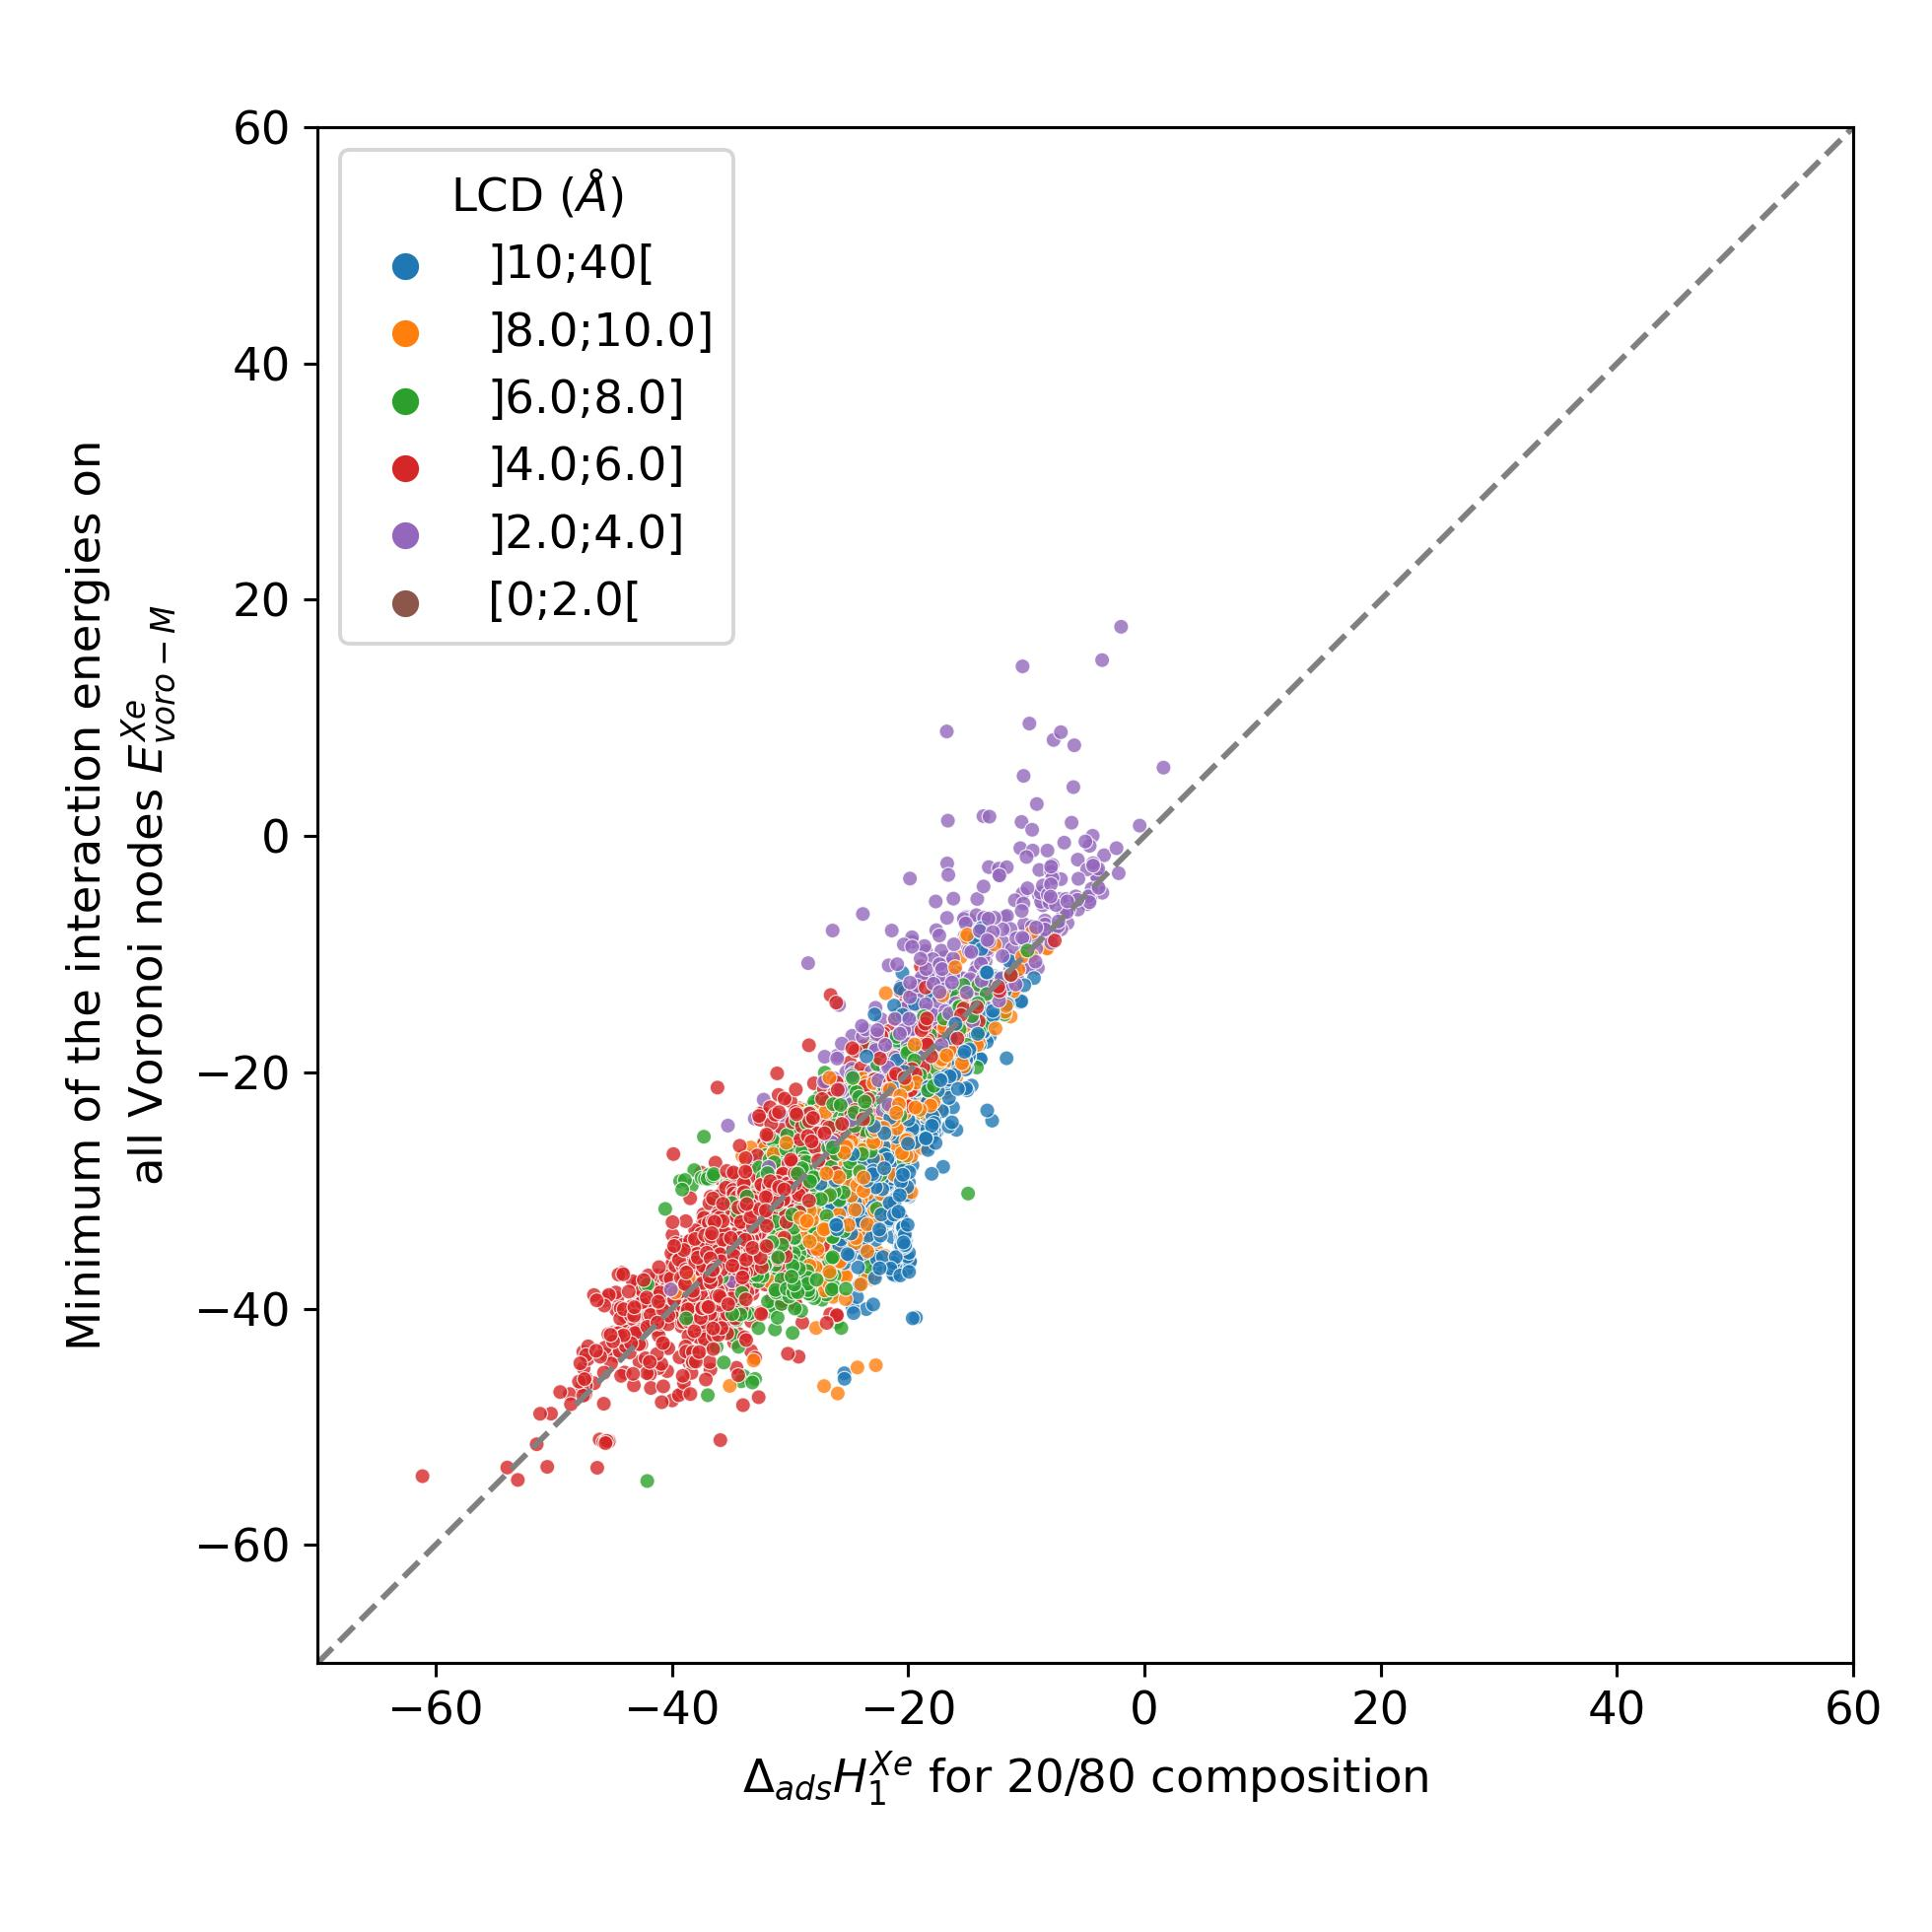
\includegraphics[width=0.32\textwidth]{figures/3-fastsim/H_Xe_2080_vs_E_voro_M_overview.jpg}
      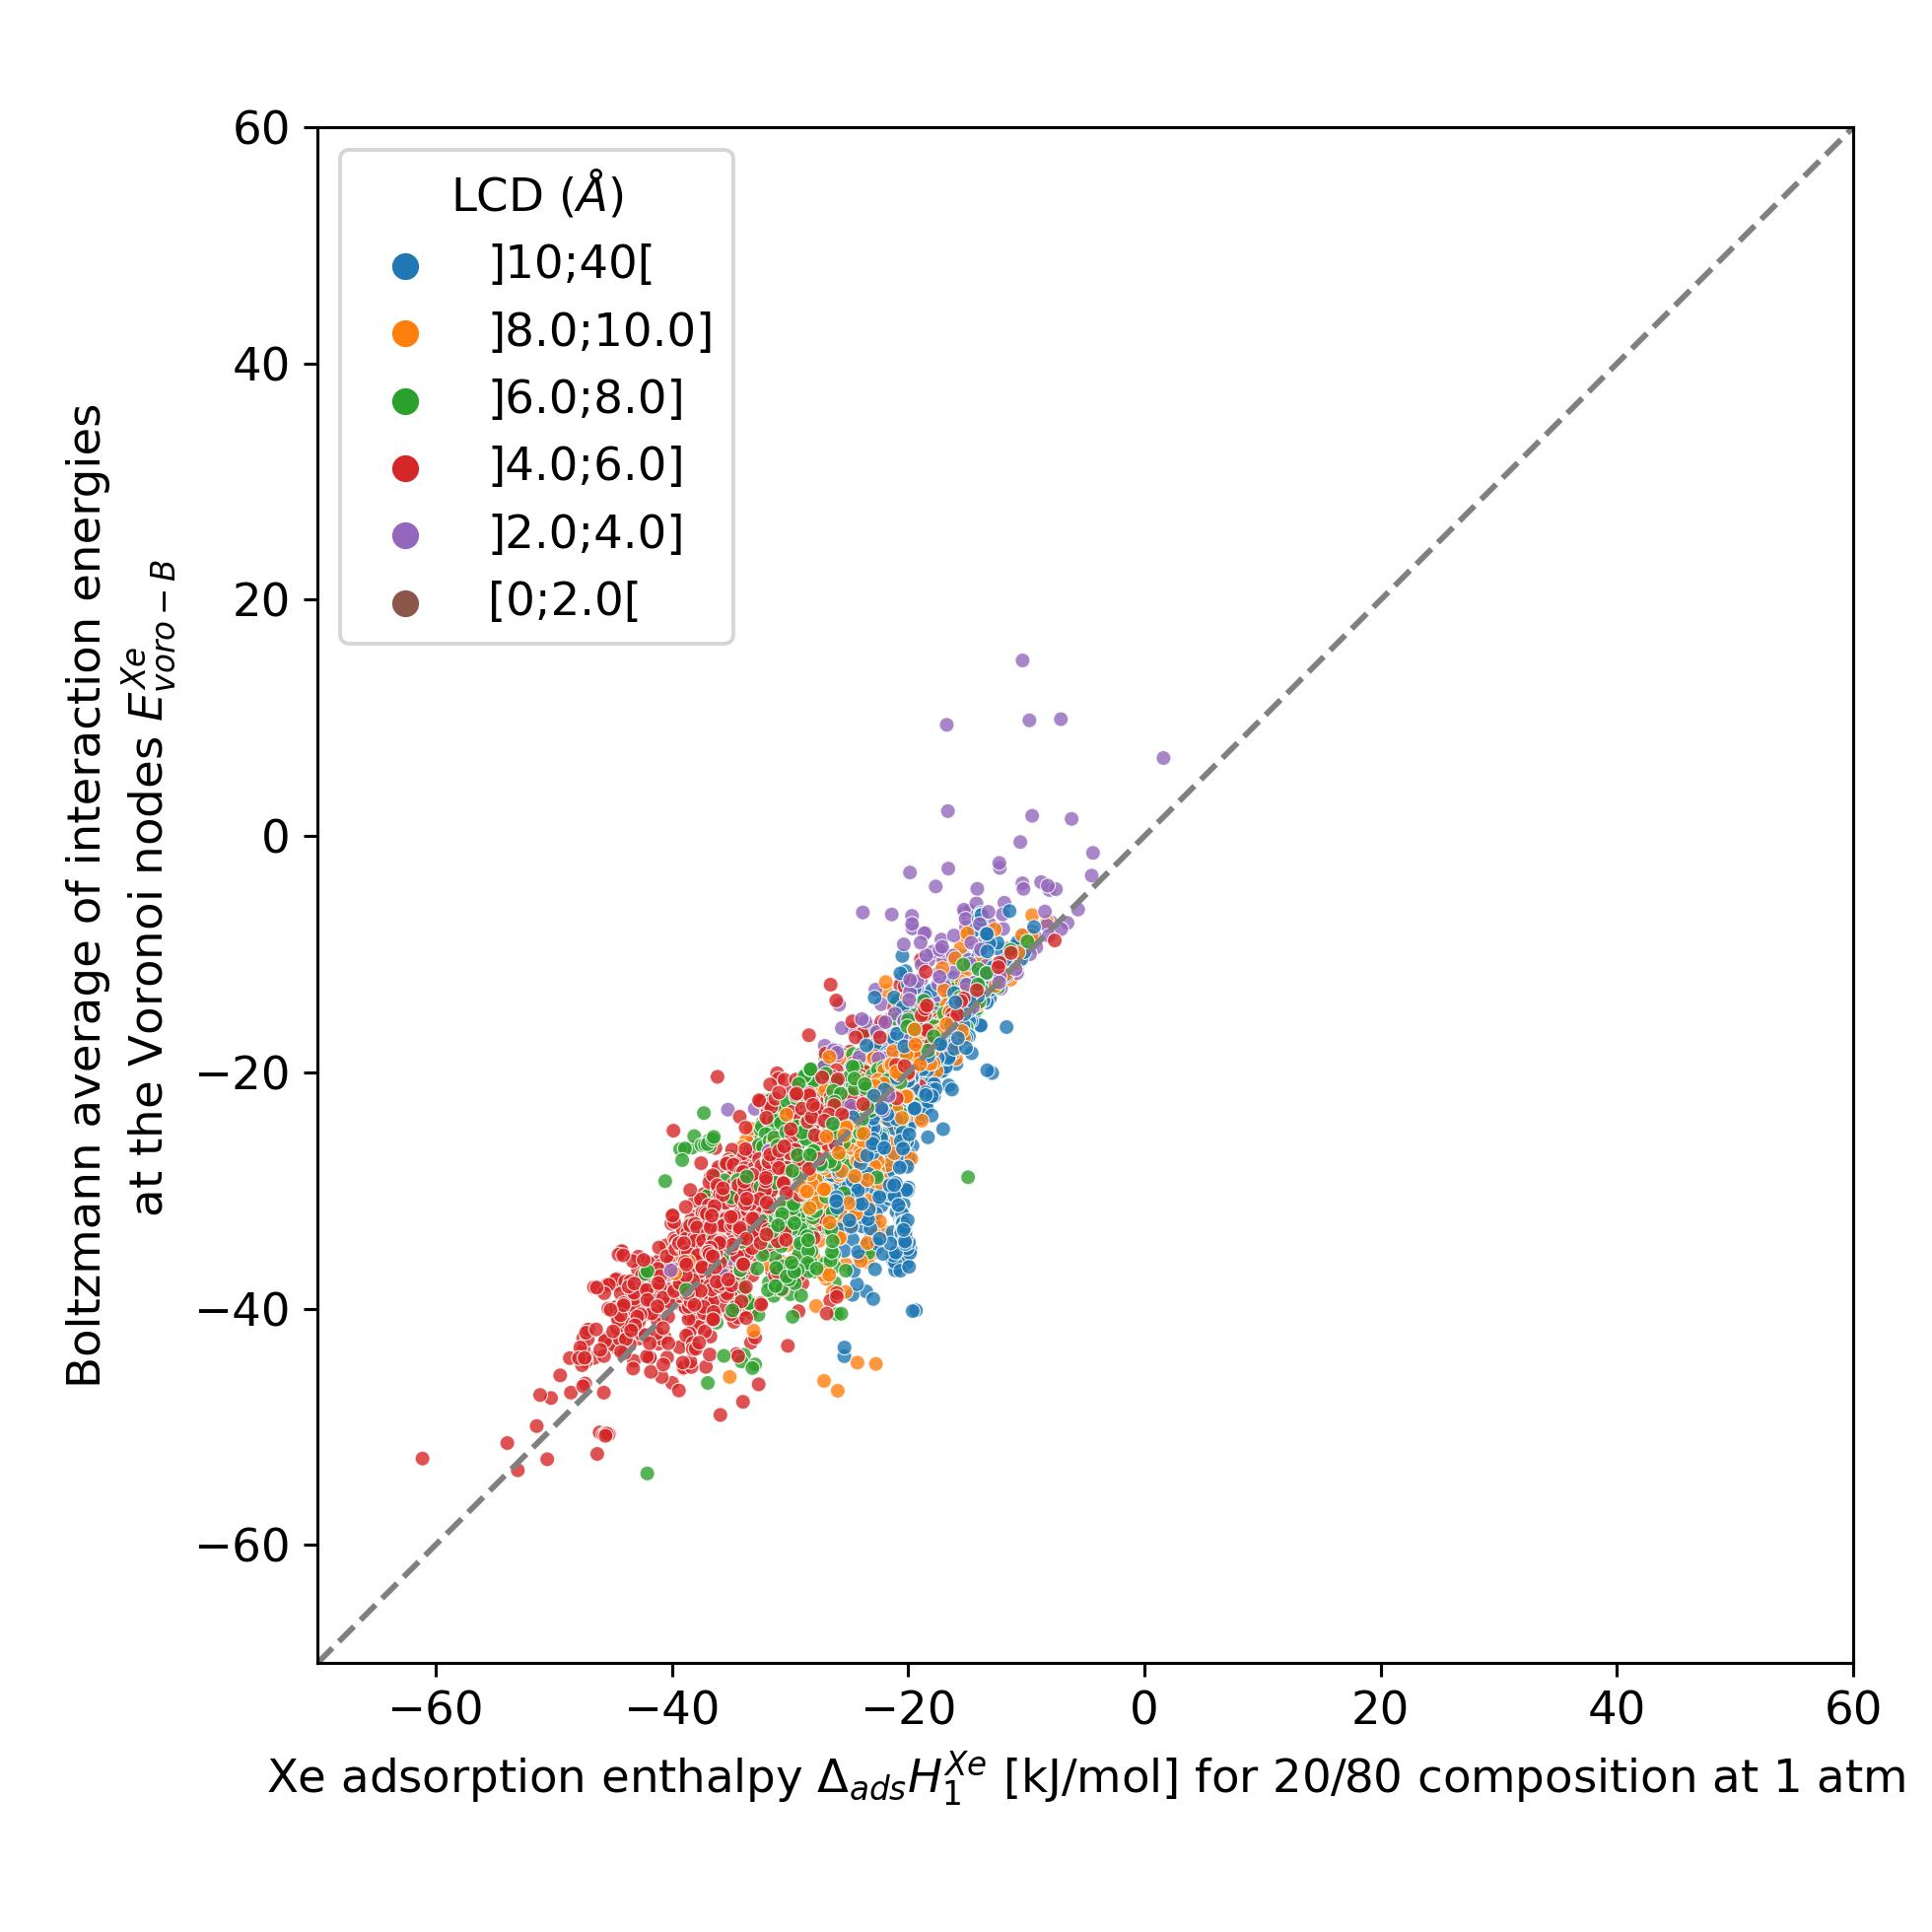
\includegraphics[width=0.32\textwidth]{figures/3-fastsim/H_Xe_2080_vs_E_voro_B_overview.jpg}
      \caption{Scatterplots of the energy descriptors $E\e{voro-A}^{Xe}$, $E\e{voro-M}^{Xe}$ and $E\e{voro-B}^{Xe}$ calculated by a Voronoi sampling compared to the enthalpies calculated by a 100k-step GCMC simulation of xenon in structures of CoRE MOF 2019. The points are labeled according to the largest cavity diameter (LCD\e{CCDC} or $D_i$) belonging to one of the intervals.}\label{fgr:compa_voro_2080}
  \end{figure}
  
At higher pressure, the adsorption enthalpy has higher values, which degrades the correlation with the Boltzmann average and the minimum of the interaction energies evaluated at the Voronoi nodes. For the averaging, the over-evaluation of the energy values make it closer to the values at higher pressure. Following this idea, we later come up with another idea of averaging with bigger weights on the higher values, a Boltzmann average with a higher temperature value that will be tested in the next chapter. 

\subsection{Performance of a Voronoi energy sampling}

We will now focus on some performance metrics associated to the Boltzmann average at the Voronoi nodes and compare it to our reference sampling, the Widom insertion with 100,000 cycles. The right plot of the Figure~\ref{fgr:compa_voro_0} compares the enthalpy computed in the Voronoi sampling with the reference adsorption enthalpy (ground truth) --- showing at the same time the largest cavity diameter for each porous framework. The correlation between the values of enthalpy is very good only for a restricted number of structures with enthalpy around \SI{-50}{\kilo\joule\per\mole}. For structures with higher enthalpy, the correlation starts to degrade, and becomes very poor for small-pore structures. For the points in purple, the largest cavity diameter is lower than the kinetic diameter of a xenon, the sampling of the Voronoi nodes is clearly insufficient. In addition, the accuracy loss on the other points (larger pores) can be explained by the fact that the pores are slightly bigger and the center of the pore is not a good approximation of adsorption site position anymore: the adsorption sites are actually closer to the pore surface than to the center of the pore. This conclusion is what prompted us to propose a new sampling scheme based on the molecular surface of the pore space, which we will detail in the next sections.

The root mean square error (RMSE) {and the mean absolute error (MAE) for Voronoi sampling are respectively \SI{6.78}{\kilo\joule\per\mole} and \SI{2.01}{\kilo\joule\per\mole}}, if we consider all structures in our set, which seems too high to be useful for screening purposes. However, the non-porous materials would be screened out \emph{a priori} in any high-throughput workflow, as they would not be of interest. We can only consider the structures with large enough cavities, higher than \SI{3.7}{\angstrom} (a bit lower than \SI{3.96}{\angstrom} Xe kinetic diameter). Thereby, {the RMSE and MAE drop respectively to \SI{2.11}{\kilo\joule\per\mole} and \SI{1.55}{\kilo\joule\per\mole}}, which can be considered acceptable for a quick estimation of the guest--host affinity, but not for accurate adsorption enthalpy calculation.

This is reinforced by the very low computational cost of the method. The Voronoi tessellation done by the Zeo++ software is extremely quick and can output the positions of the Voronoi nodes in \SI{0.28}{\second} (measured as an average over all the structures of the CoRE MOF 2019 database), on a typical workstation (a single Intel Xeon Platinum 8168 core at 2.7~\si{\giga\hertz}). While a simple Python for the energy calculation took around \SI{27}{\second} per structure, we benchmarked that a C++ optimized implementation can perform the Voronoi sampling in around \SI{0.4}{\second}. We only need to remember that this method takes a few hundred milliseconds per structure, while a Widom insertion needs approximately hundreds of seconds per structure. Voronoi sampling is therefore 2 to 3 orders of magnitude quicker than a full sampling of the pore space.

This preliminary study identified a fast method for adsorption enthalpy calculation that can be widely used in screening procedures, but has limited accuracy for quantitative prediction --- this sampling technique assumes that the nodes are close to the real, most favorable, adsorption sites, which is not always true. Or to put it differently, the adsorption sites need to be at the center of the pores, which is only true for structures with pore sizes close to adsorbate size. It raised important questions on the importance of selecting sampling points within the pore space of materials, and we wanted to develop an intermediate technique that is both fast and accurate for the prediction of adsorption enthalpy. For this purpose, we developed and optimized a new sampling technique that focuses the sampling on the surface of the material, which is expected to make up for the main flaws of the Voronoi sampling.

\section{Rapid Adsorption Enthalpy Surface Sampling (RAESS)}\label{sct:RAESS}

In this section, we describe the development of our surface sampling algorithm, with the goal of being more accurate than Voronoi sampling and faster than Widom insertion. Our initial idea is based on a series of theoretical considerations: (i) the strong adsorption sites are near the surface of the material; (ii) by changing the problem from 3D to 2D sampling we can reduce the complexity; and (iii) the algorithm can scale with the number of unique atoms in the structure (and not with the size of the unit cell), which is efficient because many porous frameworks have high symmetry. The first consideration ensures that this method will be more accurate than a Voronoi sampling, and the last two made us think that a well-optimized code would be fast. To confirm these hypotheses, we will analyze both the accuracy and the speed of this new algorithm and compare them to existing methods.

\subsection{Initial implementation}

We present here our initial implementation of the surface sampling algorithm and its  principles. This first implementation is a relatively basic one and already performs well compared to the other methods. In the next sections, we refine it with two additional features that will improve its accuracy and its speed.

This initial implementation speeds up the calculation of adsorption enthalpy in nanoporous materials by sampling interaction energies only near the surface. It is illustrated in Figure~\ref{fgr:principle}. For this purpose, a loop over all unique atoms (as defined by crystalline symmetry) is performed. And for each atom, a sphere around its position is sampled using a uniform distribution around it, these points will be called sampling points, and we can change the number of sampling points. The default radius chosen for the sampling spheres is the distance $r\e{min}=2^{1/6}\sigma_{ij}$ to the minimum of the LJ potential between atoms of type $i$ (belonging to the framework) and $j$ (the guest), corresponding to the strongest possible pair interaction (although the neighboring atoms will, of course, have an influence). After calculating the interaction energy at each of the sampled points, a Boltzmann average of these energies corresponds to a biased adsorption enthalpy, as described by the equation~\ref{eq:ads_enthalpy}.

\begin{figure}[ht]
\centering

  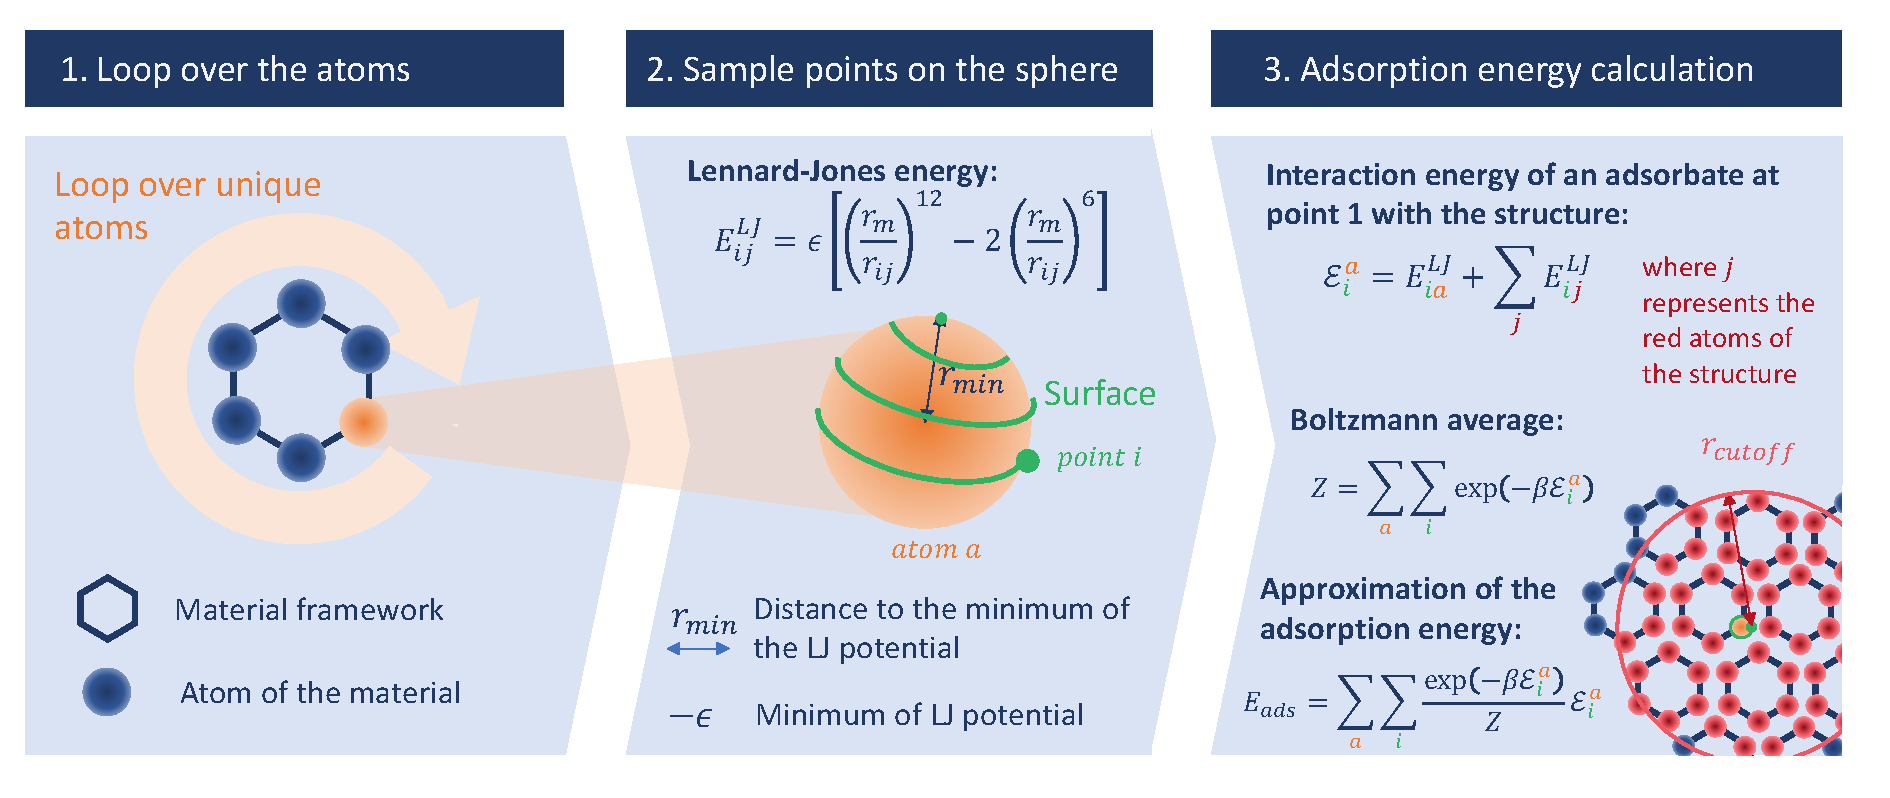
\includegraphics[clip, trim=0.6cm 0.74cm 0.78cm 0.6cm,width=0.95\linewidth]{figures/3-fastsim/Principe_screening.pdf}
  \caption{Schematic description of our surface sampling based on the three main steps of the algorithm: the loop over the unique atoms, the spiral sampling around each atom, and the energy averaging. The adsorbate is represented by the point $i$ and is moved across all the points around the unique atoms of the structure.}\label{fgr:principle}
\end{figure}

In order to validate the accuracy of the approximation made using this sampling, we applied this algorithm with 300,000 sampling points per unique atom. The results are illustrated by the Figure~\ref{fgr:surface_sampling}. There is a good numerical agreement with the reference calculations, {the RMSE and MAE are only around \SI{0.90}{\kilo\joule\per\mole} and \SI{0.66}{\kilo\joule\per\mole}} considering all the structures from the database. Moreover, there is no noticeable difference of RMSE when considering the structures with a pore size above \SI{3.7}{\angstrom} (as determined by the LCD\e{CCDC}). Unlike Voronoi sampling, this method gives a consistent accuracy across all the structures of the database with a lower error. The fact that the {RMSE} error is below \SI{1}{\kilo\joule\per\mole} is quite promising, and validates our intuition that this new sampling technique can be an intermediate between to the two previous methods (Voronoi and Widom).

\begin{figure}[ht]
  \centering
  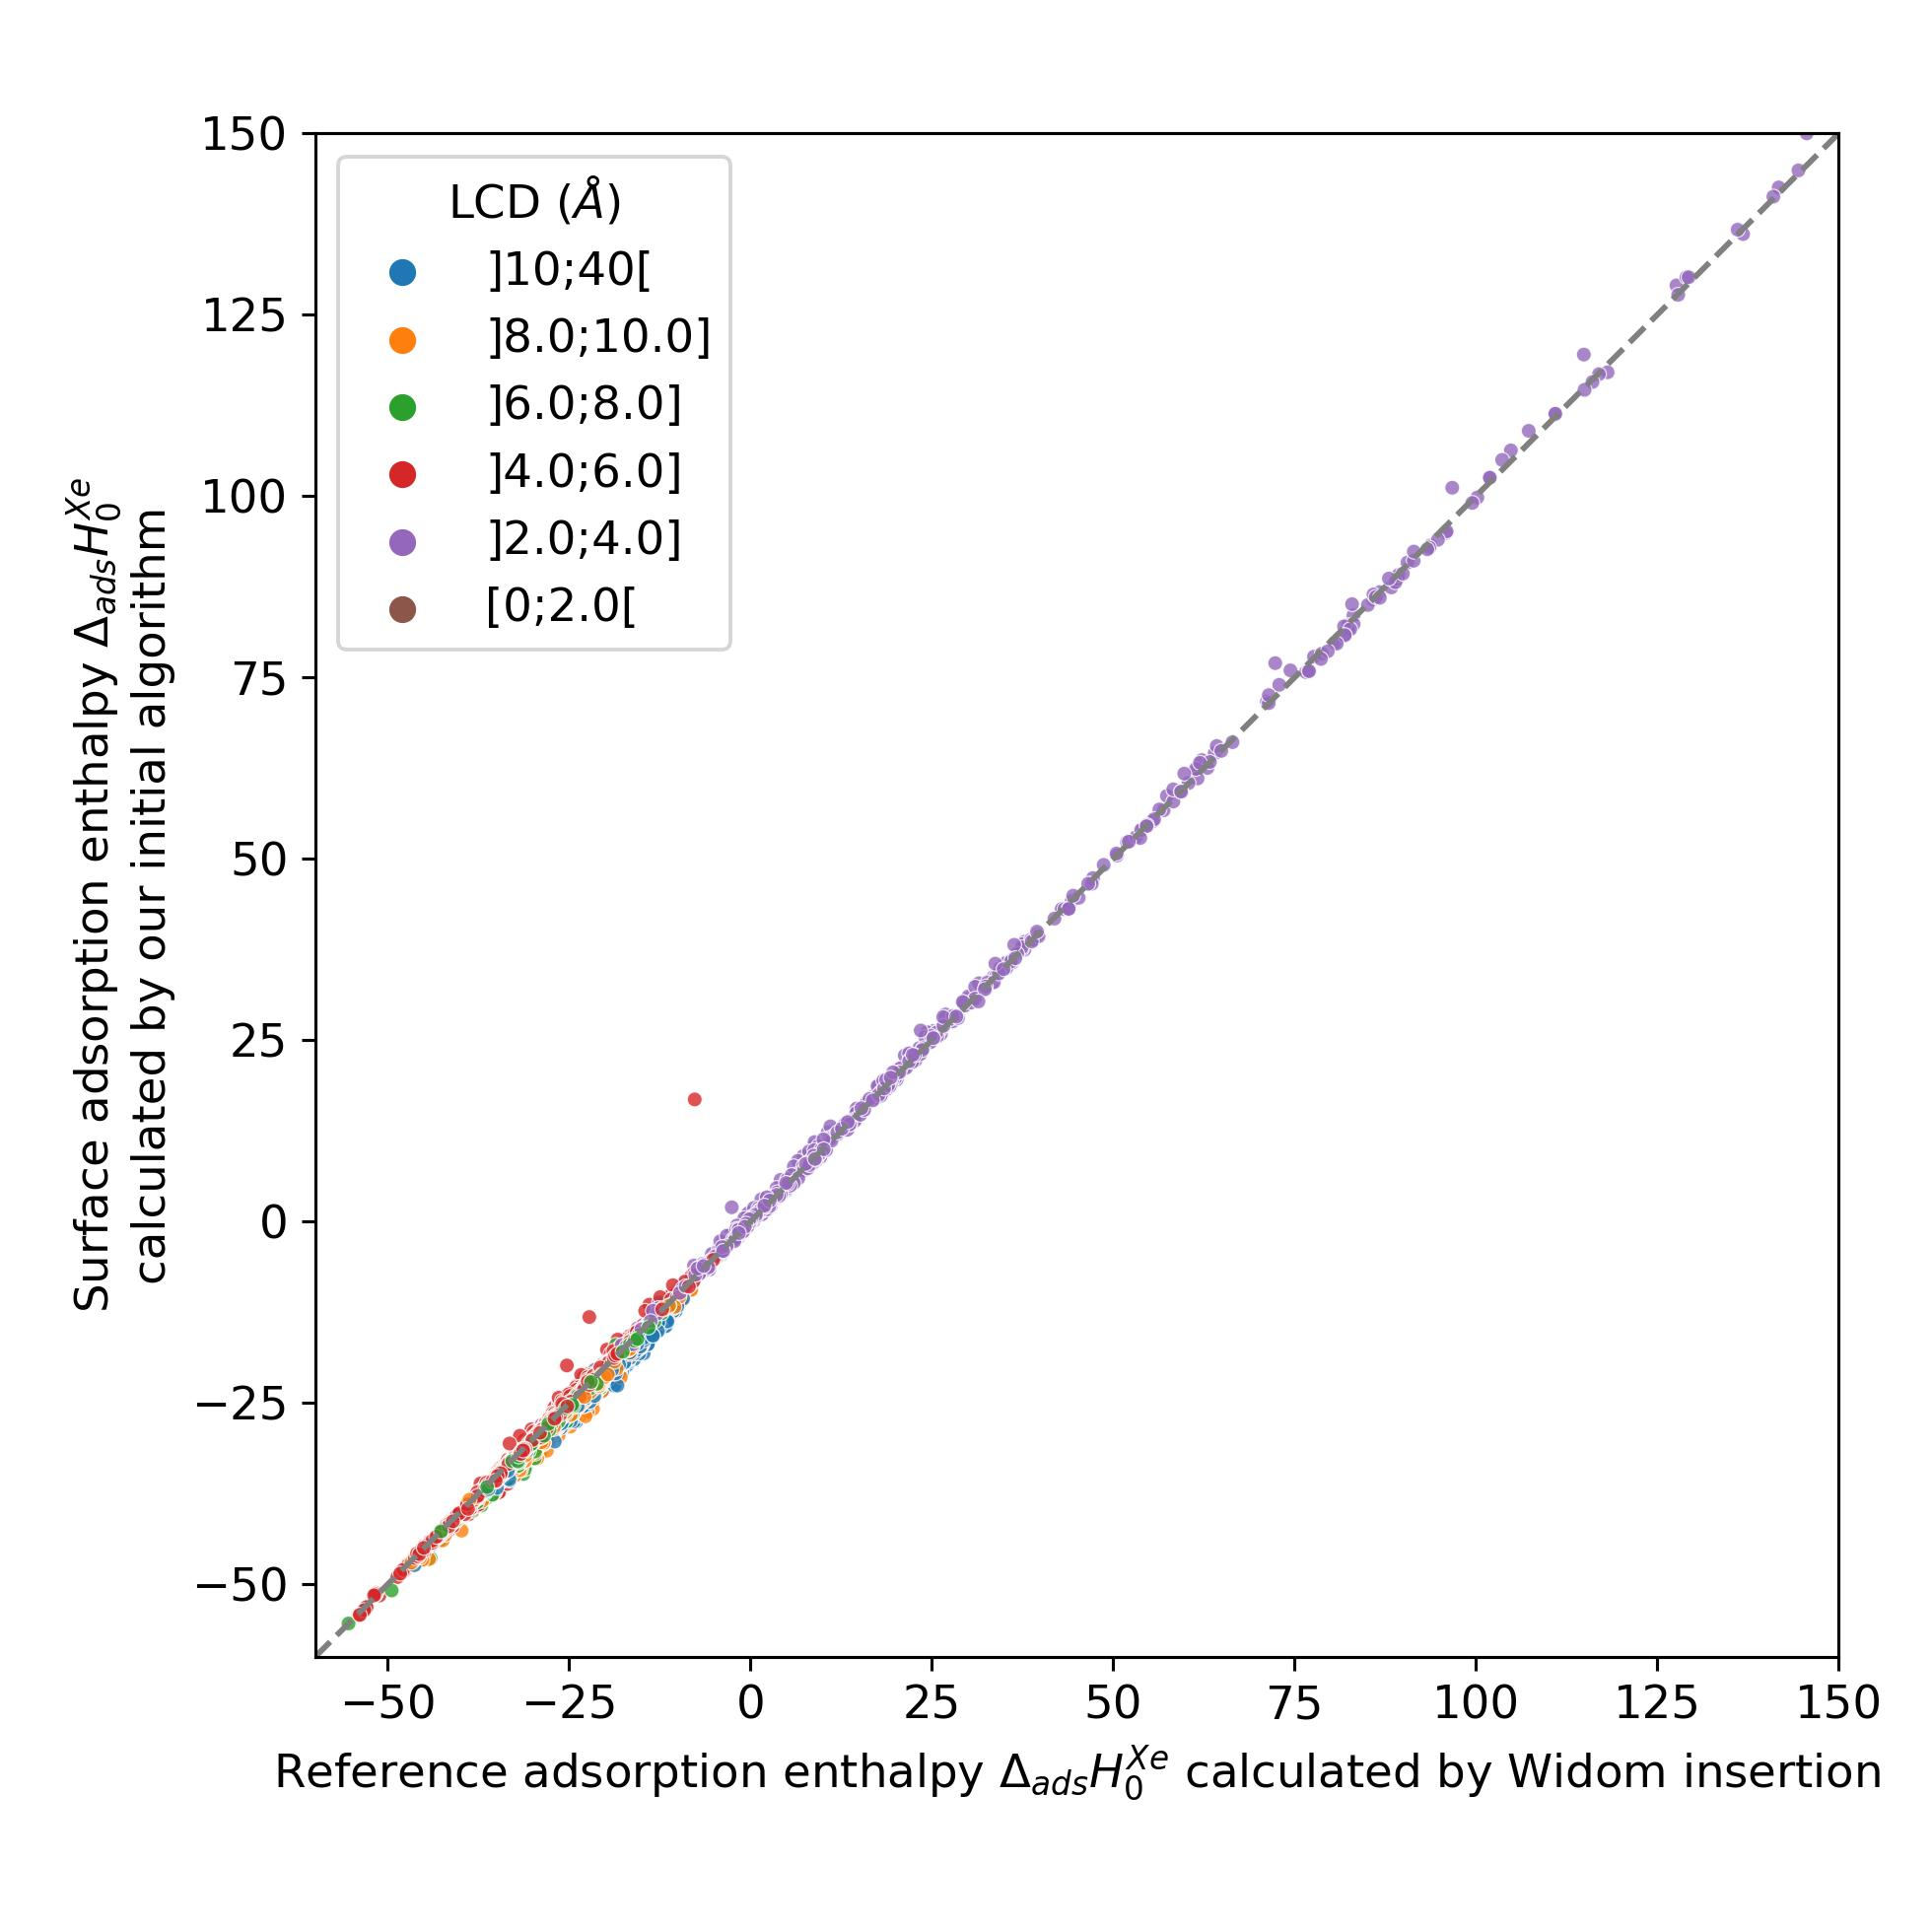
\includegraphics[width=0.45\linewidth]{figures/3-fastsim/H_Xe_widom_vs_H_Xe_surface_spiral_overview.jpg}
  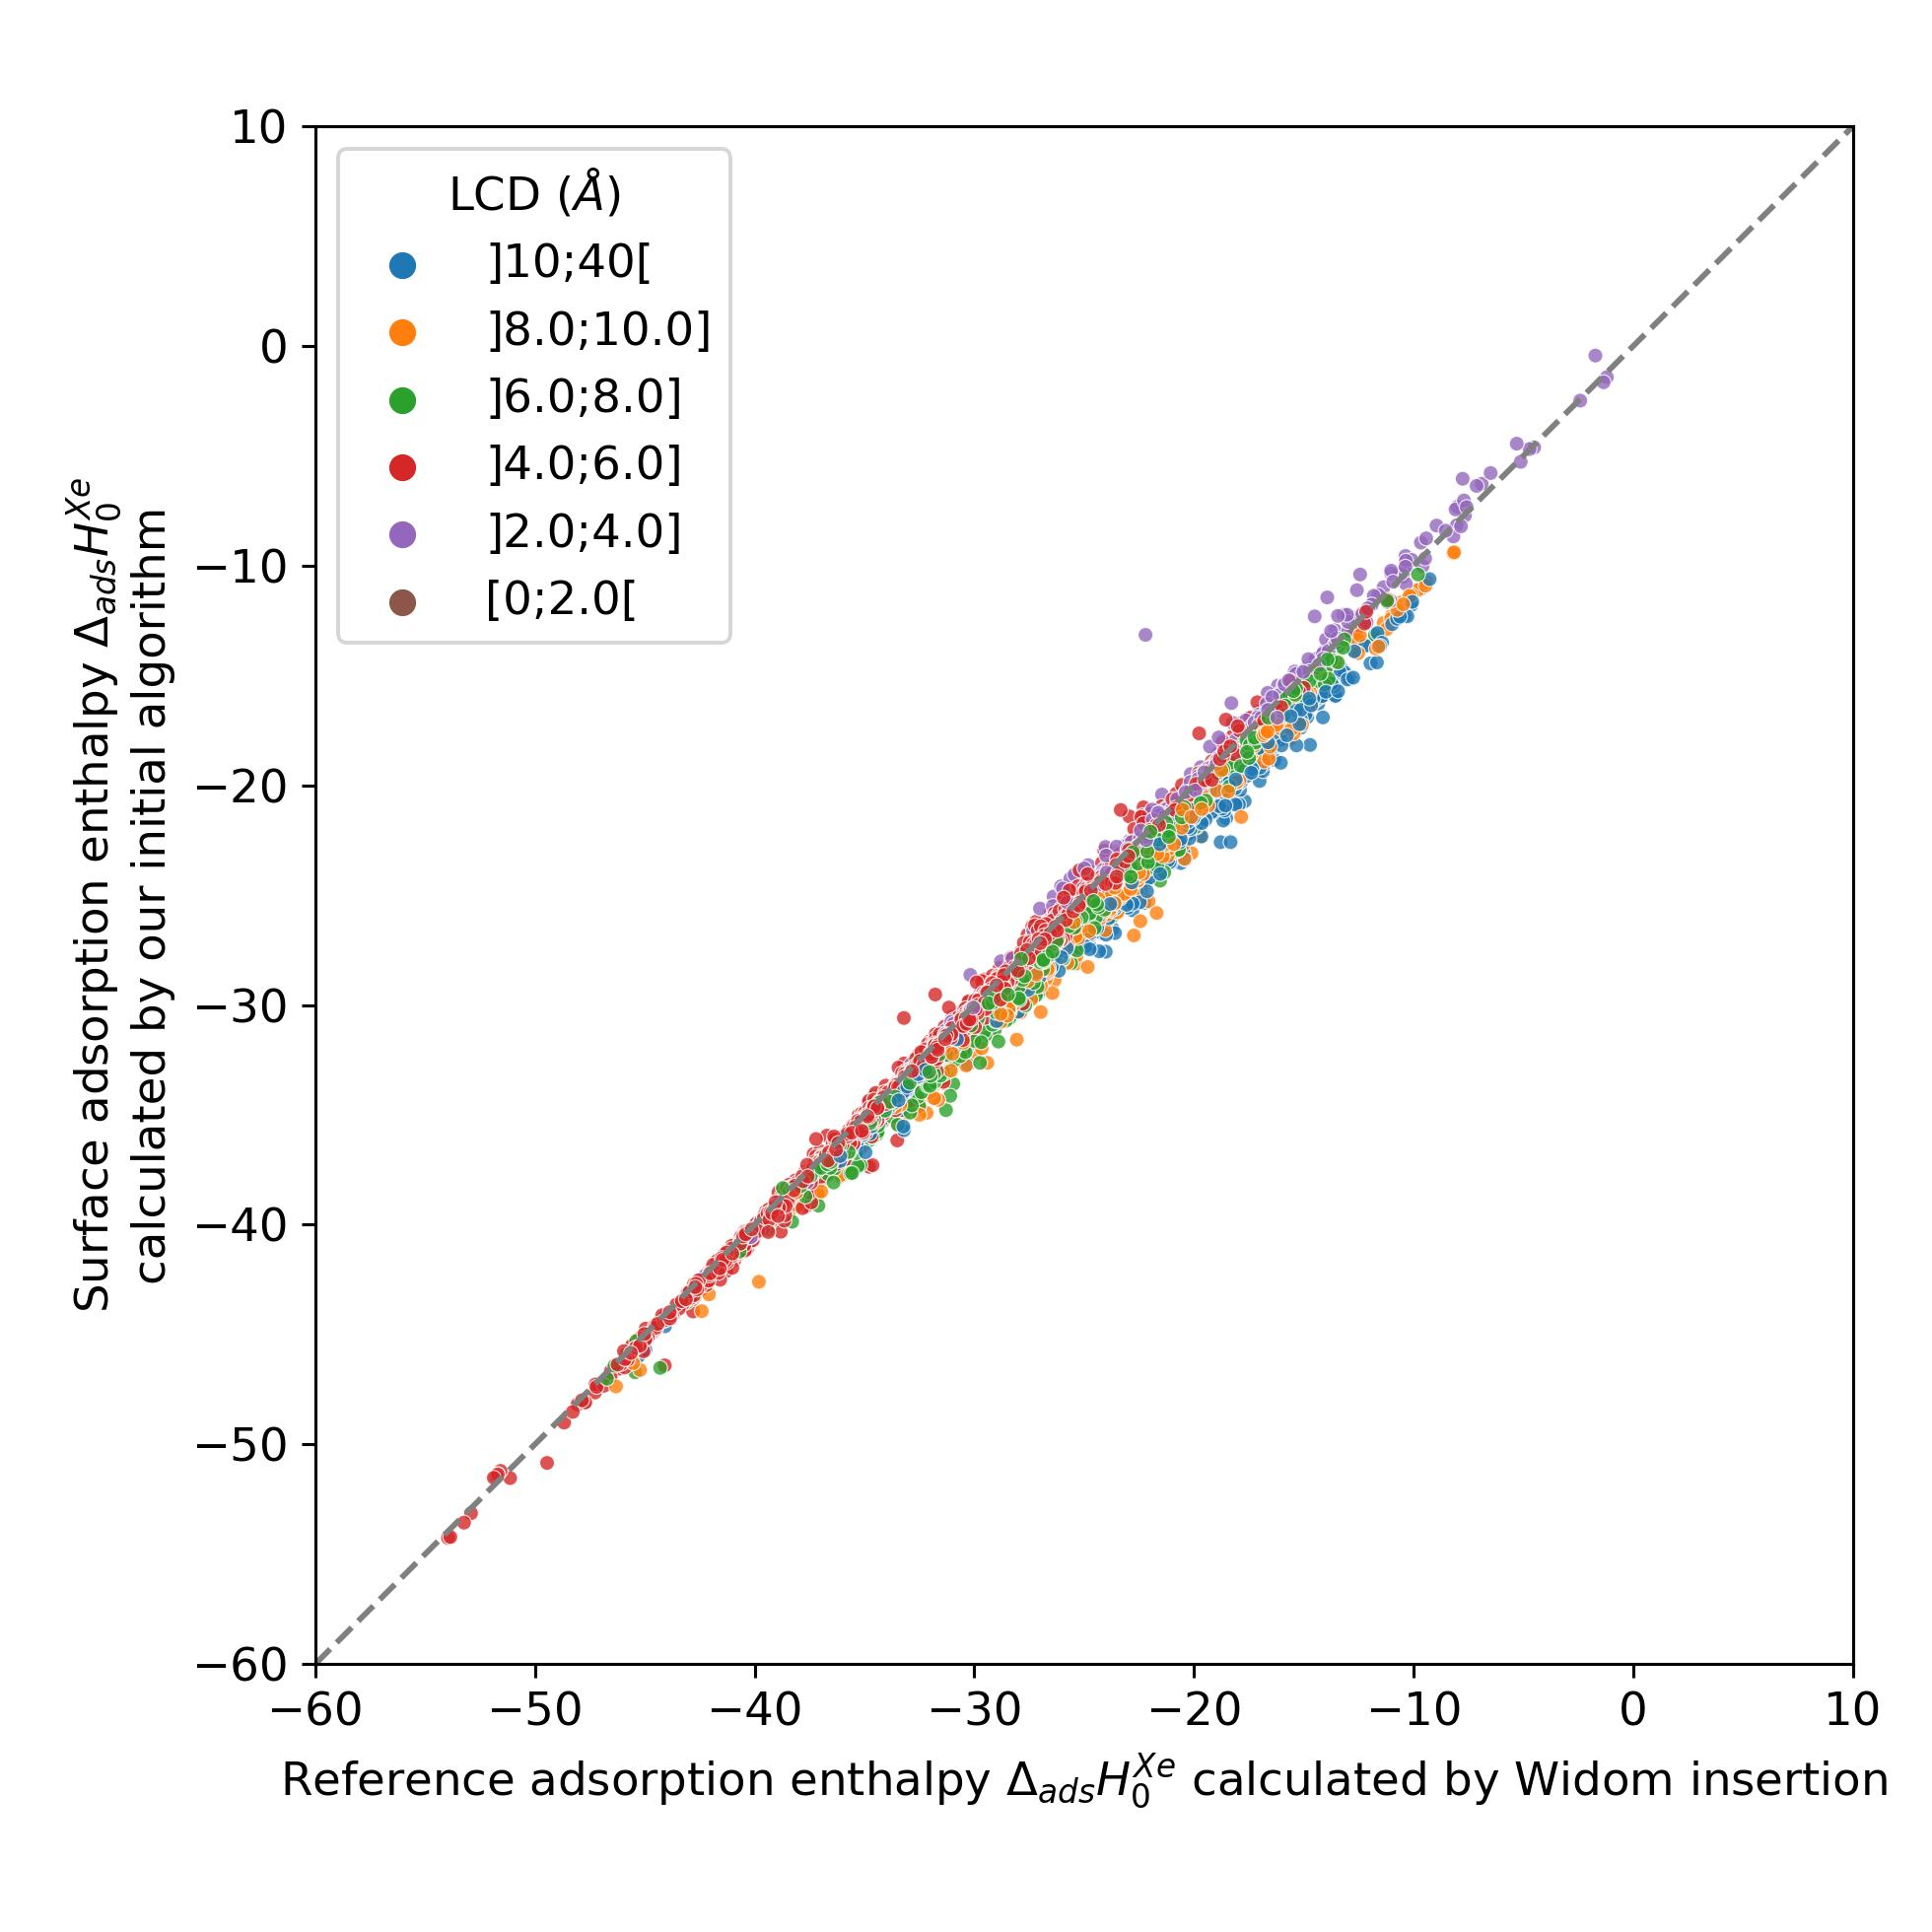
\includegraphics[width=0.45\linewidth]{figures/3-fastsim/H_Xe_widom_vs_H_Xe_surface_spiral_zoom.jpg}
    \caption{Scatterplots of the xenon surface adsorption enthalpy calculated by an initial implementation of the RAESS algorithm as a function of the xenon adsorption enthalpy calculated by a 100k-step Widom insertion simulation using two value windows. The second plot zooms on the negative values corresponding to the most selective materials.}\label{fgr:surface_sampling_init}
\end{figure}

After proving the good accuracy of the method, we are now exploring the computation time required. We see on Figure~\ref{fgr:convergence} that the method reaches an RMSE below \SI{1.0}{\kilo\joule\per\mole} very quickly for an average CPU time of \SI{1.2}{\second}, corresponding to 2,000 sampling points per atom. This is far less than the \SI{150}{\second} required for a Widom insertion to be near its plateau value (converges to zero), for an RMSE of \SI{0.10}{\kilo\joule\per\mole} with 12,000 cycles. Moreover, the Widom insertion needs around \SI{14}{\second} to reach a similar RMSE of \SI{1.0}{\kilo\joule\per\mole}, which is still slower than the surface sampling. We can conclude that this initial implementation of the surface sampling is faster than a standard Widom insertion, with a good accuracy.

These results on the convergence speed and the limit values of the error can be simply rationalized by the nature of each sampling. In a surface sampling, the sampled points are biased toward the most attractive points of adsorption for the xenon, which explains the fact that the value converges very quickly because the most influential terms of the Boltzmann average are quickly gathered. However, in a Widom insertion every point of the space has equal chances of being sampled, which is extremely close to the definition of the enthalpy but requires much more time to randomly sample a very attractive adsorption site. The surface sampling by its biased nature, however, will inherently be less accurate since not all points are considered equally and sometimes the most optimal adsorption site could be missed, because it could in some cases be further from the sampled surface. 

\begin{figure}[ht]
  \centering
    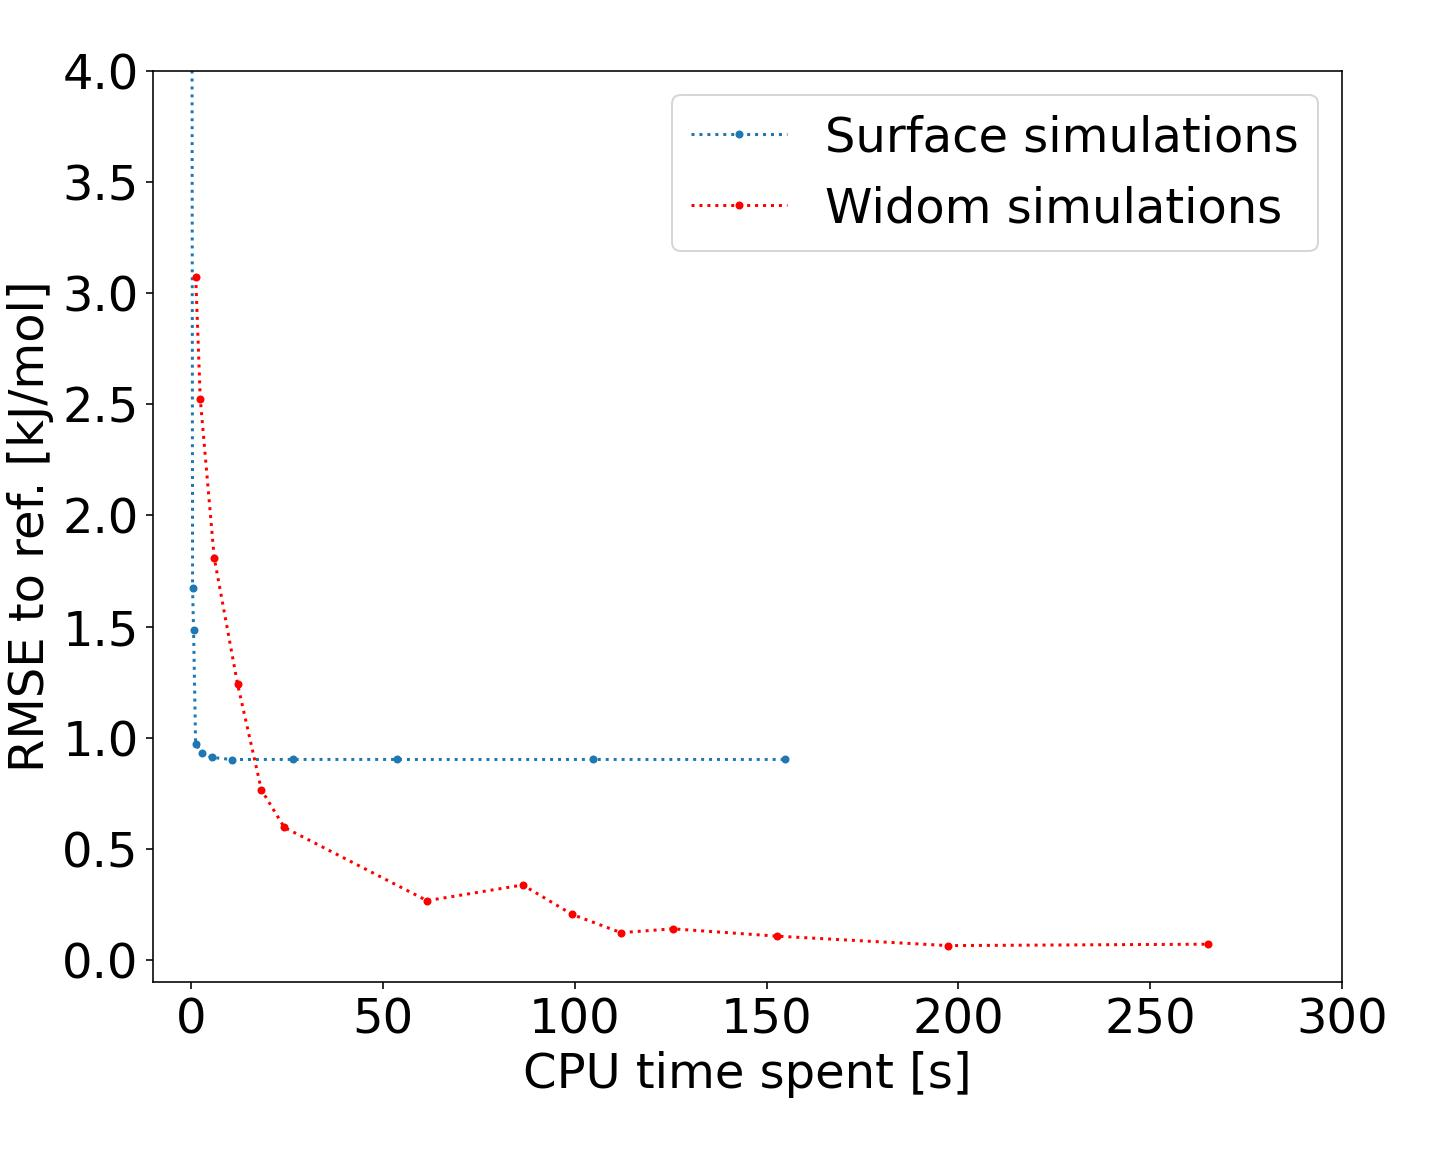
\includegraphics[width=0.7\linewidth]{figures/3-fastsim/time_rmse.jpeg}
    \caption{Convergence plot of the RMSE on the adsorption enthalpy for our algorithm (blue) compared to a 100k-step Widom insertion simulation (red) for xenon adsorption in {all} structures of the CoRE MOF 2019 database.}\label{fgr:convergence}
  \end{figure}
  

However, this initial implementation of the method is slower than a Voronoi sampling that only needs to sample around 1,600 points on average, instead of 13,000 sampled points on average (if we multiply by the average number of unique atoms). The sampling part would take approximately \SI{0.15}{\second} and the Voronoi nodes generation \SI{0.28}{\second}, so our surface sampling algorithm remains 2 to 3 times slower (implemented in an identical compiled language, in this case C++). In order to improve the accuracy and performance, we have further tweaked the surface sampling method, adjusting the size of the sampling sphere and adopting a fast rejection criterion. The rejection of high-energy points with little contribution to the final enthalpy value can reduce the simulation time, whereas the size of the sampling sphere can improve the accuracy. The initially chosen sphere size is only taking account of the interaction with the closest atom, we therefore chose to set it at the minimum of Lennard-Jones potential. However, the interaction with the neighboring atoms can further stabilize the adsorbate, sampling further from this minimum could in consequence increase the accuracy of our surface sampling method.

\subsection{Performance improvement of the algorithm}

\subsubsection{Size of the sampling sphere}

The validity of the initial algorithm is based on the assumption that the adsorption site is at the minimum of the Lennard-Jones potential. It will only perform well if the closest atom contributes to almost all the interaction, but in real frameworks other neighboring atoms contribute to the host/guest interaction as well. We have found that in vast majority of materials, the adsorption sites are located farther apart compared to the LJ potential minimum, in order to maximize the contribution of all atoms --- and because of the dissymmetry of the interaction potential well. In order to see if this could be introduced in our algorithm, we implemented a parameter $\lambda$, and the sampling sphere radius is now defined by $R_{\lambda} = \lambda \sigma$, where $\sigma$ is the distance at which the LJ potential is zero. If $\lambda=2^{1/6}$, we fall back to our initial definition of the sampling sphere, and the adsorbent is at the minimum of the LJ potential of the atom. If $\lambda=1$, the sampling sphere is at the zero of the LJ potential, and by increasing this parameter, we can check if our intuition was right.

\begin{figure}[ht]
\centering
  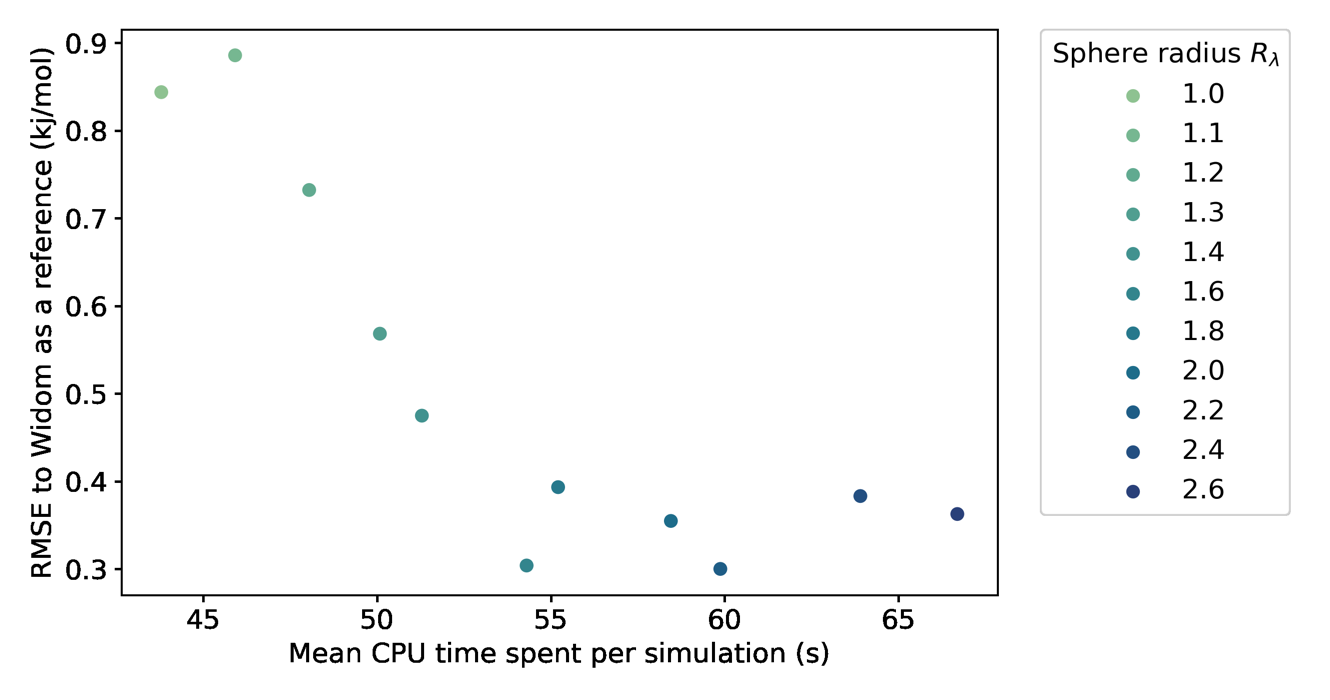
\includegraphics[width=0.7\linewidth]{figures/3-fastsim/sphere_size_optimisation.png}
  \caption{Influence of the sampling sphere radius $R_{\lambda}$ on the average CPU time required for a simulation of 100k sampling points and the RMSE, compared to the reference adsorption enthalpy. The averaging is done only on the structures with a largest cavity diameter (LCD\e{CCDC}) higher than \SI{3.7}{\angstrom}.}\label{fgr:radius}
\end{figure}

Because we have no physical model that would predict the optimal value of the sampling sphere, we followed a statistical approach. We studied the influence of the $\lambda$ parameter on both the accuracy and the computation time, and the results are represented on Figure~\ref{fgr:radius}. The RMSE turns out to be relatively high around \SI{0.90}{\kilo\joule\per\mole} for radius sphere lower than the $r\e{min}$, it then decreases for larger values of radius to reach a plateau around \SI{0.35}{\kilo\joule\per\mole}. We confirm that by increasing the sampling sphere radius we can improve the accuracy of our algorithm, and find that for values of $\lambda$ higher than $1.6$, the accuracy is stabilized. We also find that increasing the sphere radius negatively impacts the computational efficiency, since it increases the number of neighbors considered in the energy calculation.

By choosing an optimal sampling sphere, we can more than halve the error, while increasing the computation time by around 20 percent, when comparing the case $\lambda=1.6$ with $\lambda=1.1$ (close to $r\e{min}$). In most cases, it will be an acceptable trade-off. However, in a case where the computation time is crucial, like in a rapid screening, the optimal choice might not be to increase the sampling sphere at $\lambda=1.6$ but to have it lower at $\lambda=1.4$ or $\lambda=1.2$, and have an RMSE around \SI{0.5}{\kilo\joule\per\mole} --- still quite acceptable. The new scale parameter introduced in this section can therefore be tweaked to serve the users' purpose, whether it is to focus on the accuracy or to optimize the computation speed. {If one wants to use it on a completely different database in very different conditions, then one can either choose a default value that works fine (\emph{e.g.} $\lambda=1.4$) or one can optimize the parameter on a small diverse sample of the unseen data. }

\subsubsection{Rejection condition}\label{sct:rejection_condition}

As shown above, our algorithm has better accuracy than Voronoi sampling, but its initial implementation was several times slower, which could be unsuitable for screening applications in high-throughput workflows, where the number of structures to be screened can reach one million or more. To reduce the computational expense, we thought of rejecting the points with little contribution to the final enthalpy, i.e., the largely positive interaction energies that would vanish in the exponential of the  Boltzmann average.

\begin{figure}[ht]
\centering
  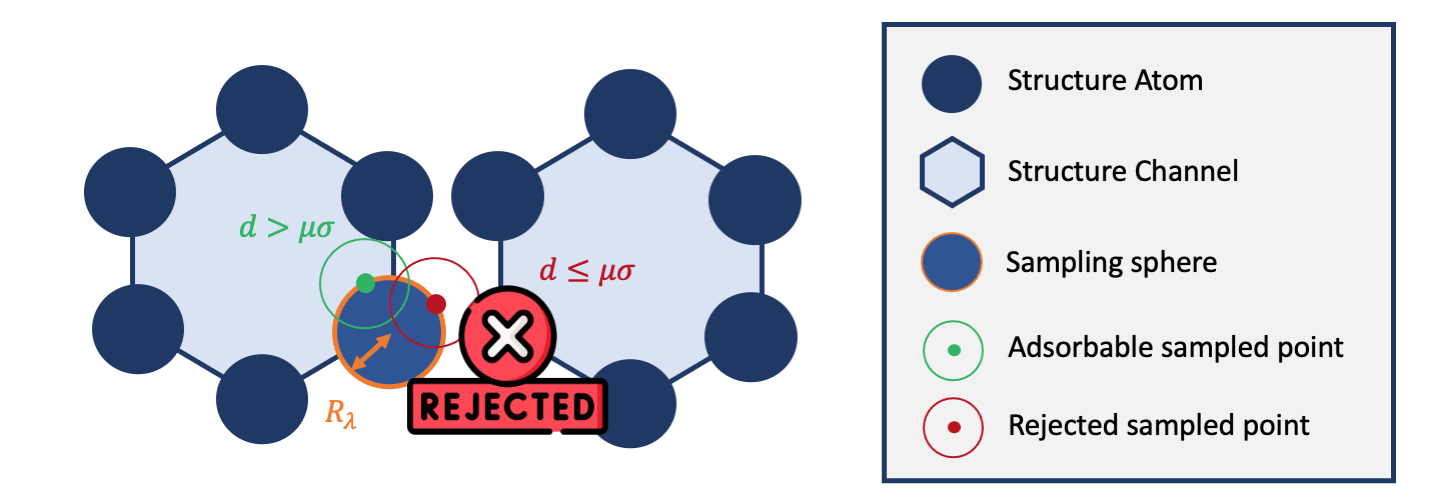
\includegraphics[width=\linewidth]{figures/3-fastsim/rejection_sampling_sphere.png}
  \caption{Simplified representation of the principle of rejection condition and the concept of sampling sphere inside 2D channels of a nanoporous material.}\label{fgr:feature}
\end{figure}

Inspired by typical methods for accessible surface calculation, we implemented a hard sphere rejection condition based on the distance to neighbors. If the adsorbate is too close to another atom of the structure, the sampling point is rejected, i.e., its energy is not calculated (or considered to be infinite). We based this distance threshold on the $\sigma_{ij}$ parameter of the Lennard-Jones potential. To determine the optimal threshold, we introduced a factor $\mu$ with real values between 0 and 1, that changes the size of the hard sphere rejection condition. If the guest--host distance is lower than $d_{\mu} = \mu \times \sigma$, then the point is rejected. If $\mu = 0$, then there is no rejection condition. And if $\mu = 1$, we reject all points with a positive energy interaction to at least one atom of the structure. This condition could be a bit strong and points with non-negligible contribution would end up rejected. This rejection condition is schematically represented on Figure~\ref{fgr:feature}.

This rejection condition is expected to speed up the calculation, since the energy calculation is avoided for the rejected sampling points. The energy calculation accounts for the largest portion of the CPU time spent in the surface sampling. For the structure \texttt{KAXQIL}\autocite{Banerjee_2012}, the Lennard-Jones potential calculation represents up to $90\%$ of the calculation time for 100,000 sampling points per sphere (with the initial algorithm). The higher the factor $\mu$, the more rejections there would be. But, if too many points are rejected, the accuracy would drop. Here again, we used a statistical analysis to determine the optimal value of $\mu$, making our sampling faster without compromising the accuracy of the enthalpy calculation. The results are displayed on Figure~\ref{fgr:rejection}.

\begin{figure}[ht]
\centering
  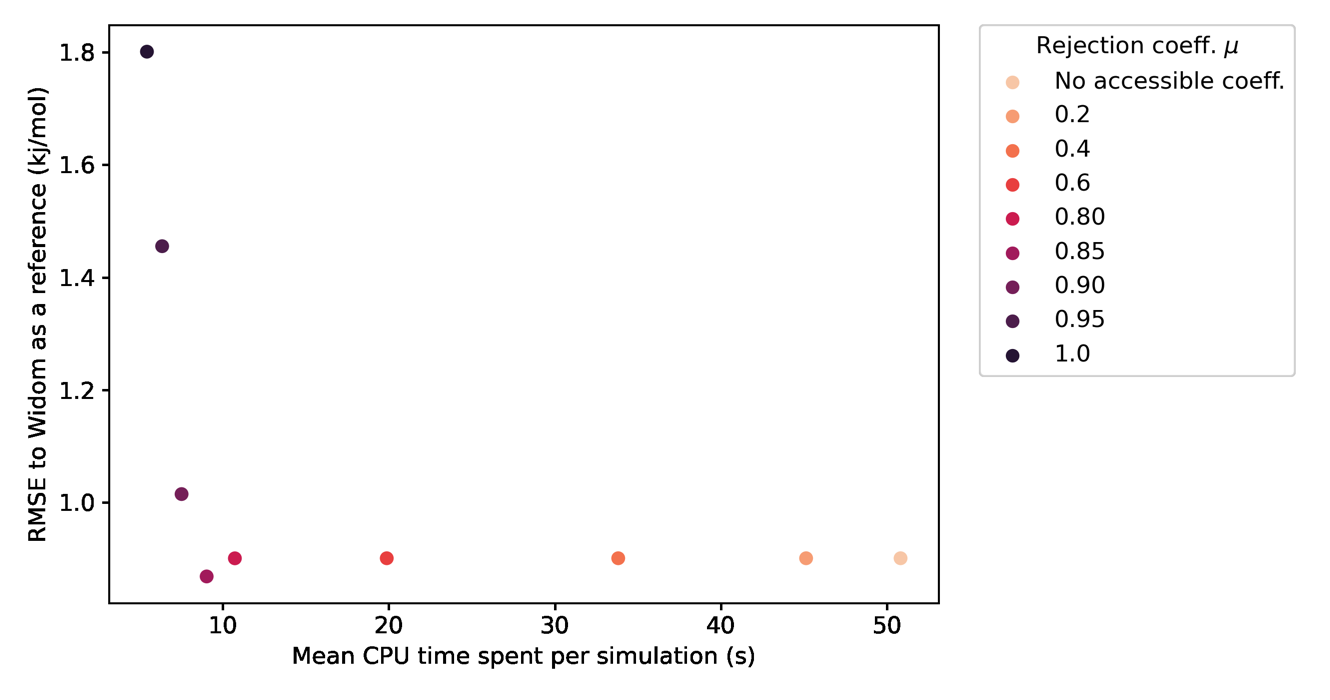
\includegraphics[width=0.7\linewidth]{figures/3-fastsim/rejection_coeff_optimisation.png}
  \caption{Influence of the rejection coefficient $\mu$ on the average CPU time required for a simulation of 100k sampling points and the RMSE compared to the reference adsorption enthalpy. The averaging is done only on the structures with a largest cavity diameter (LCD\e{CCDC}) superior to \SI{3.7}{\angstrom}. }\label{fgr:rejection}
\end{figure}

The values of RMSE and time on Figure~\ref{fgr:rejection} are averaged only on the most interesting structures for xenon adsorption (LCD\e{CCDC} $\geq$ \SI{3.7}{\angstrom}). For $\mu\leq 0.85$, increasing the value of $\mu$ improves the speed of the calculation without changing the RMSE.\footnote{In fact, what we observe is a deterioration of the accuracy for structures with small pores because the probability of rejection in a confined space is really high and all sampled points end up rejected. But these points are not considered if we apply the condition on the cavity size (LCD\e{CCDC} $\geq$ \SI{3.7}{\angstrom}).} For high values of $\mu$, the rejection condition is too strong and we reject points with non-negligible contribution to the overall enthalpy. The RMSE increases as a consequence. If we want to keep the accuracy unchanged, the optimal value is therefore $\mu \simeq 0.85$, because it gives the lowest computation time with a similar RMSE. We note that it would be possible, in specific cases, to explore higher values of $\mu$ that trade a bit more accuracy in exchange for further speed gains.

For the simulations considered in Figure~\ref{fgr:rejection}, the use of a rejection condition $\mu = 0.85$ makes the simulation four times faster than the standard algorithm. As we will see in the next section, the combination of optimal values for the $\lambda$ and $\mu$ parameters generates an algorithm with very interesting performance compared to Voronoi sampling or Widom insertion.


\subsection{Final surface sampling implementation}\label{sct:final_sampling}

\subsubsection{Performance comparison}

For the calculation of adsorption enthalpy, our proposed surface sampling method is a good compromise between the accuracy of Widom insertion (full sampling of the porous space) and the speed of a less accurate method such as Voronoi sampling. The performance of our algorithm, including the two new features (sampling sphere scaling and rejection criterion) is illustrated in Figure~\ref{fgr:sumup}, where we can see the improvement brought by each feature and how it compares to reference simulations. All CPU times are calculated using the smallest possible number of sampling points so that the respective algorithms reach convergence. With the implementation of a rejection condition, we find that surface sampling is even quicker than Voronoi sampling. Moreover, the increase of the size of the sampling sphere makes the surface sampling much more accurate, reaching an RMSE of \SI{0.33}{\kilo\joule\per\mole} {and an MAE of \SI{0.21}{\kilo\joule\per\mole}}. The ideal set of parameters, determined for porous materials from the CoRE MOF 2019 database, is $(\lambda = 1.6, \mu = 0.85)$ in order to combine the lowest error and smallest computational cost. By combining both of these new features to the algorithm, we have a final surface sampling method with an RMSE of \SI{0.33}{\kilo\joule\per\mole} and an average computation time of \SI{0.34}{\second} per structure. According to the data represented in Figure~\ref{fgr:sumup}, it is about 6 times more accurate and {$26$\%} faster than Voronoi sampling, and it is also about 430 times faster than a Widom insertion with 12k cycles.

\begin{figure}[ht]
  \centering
  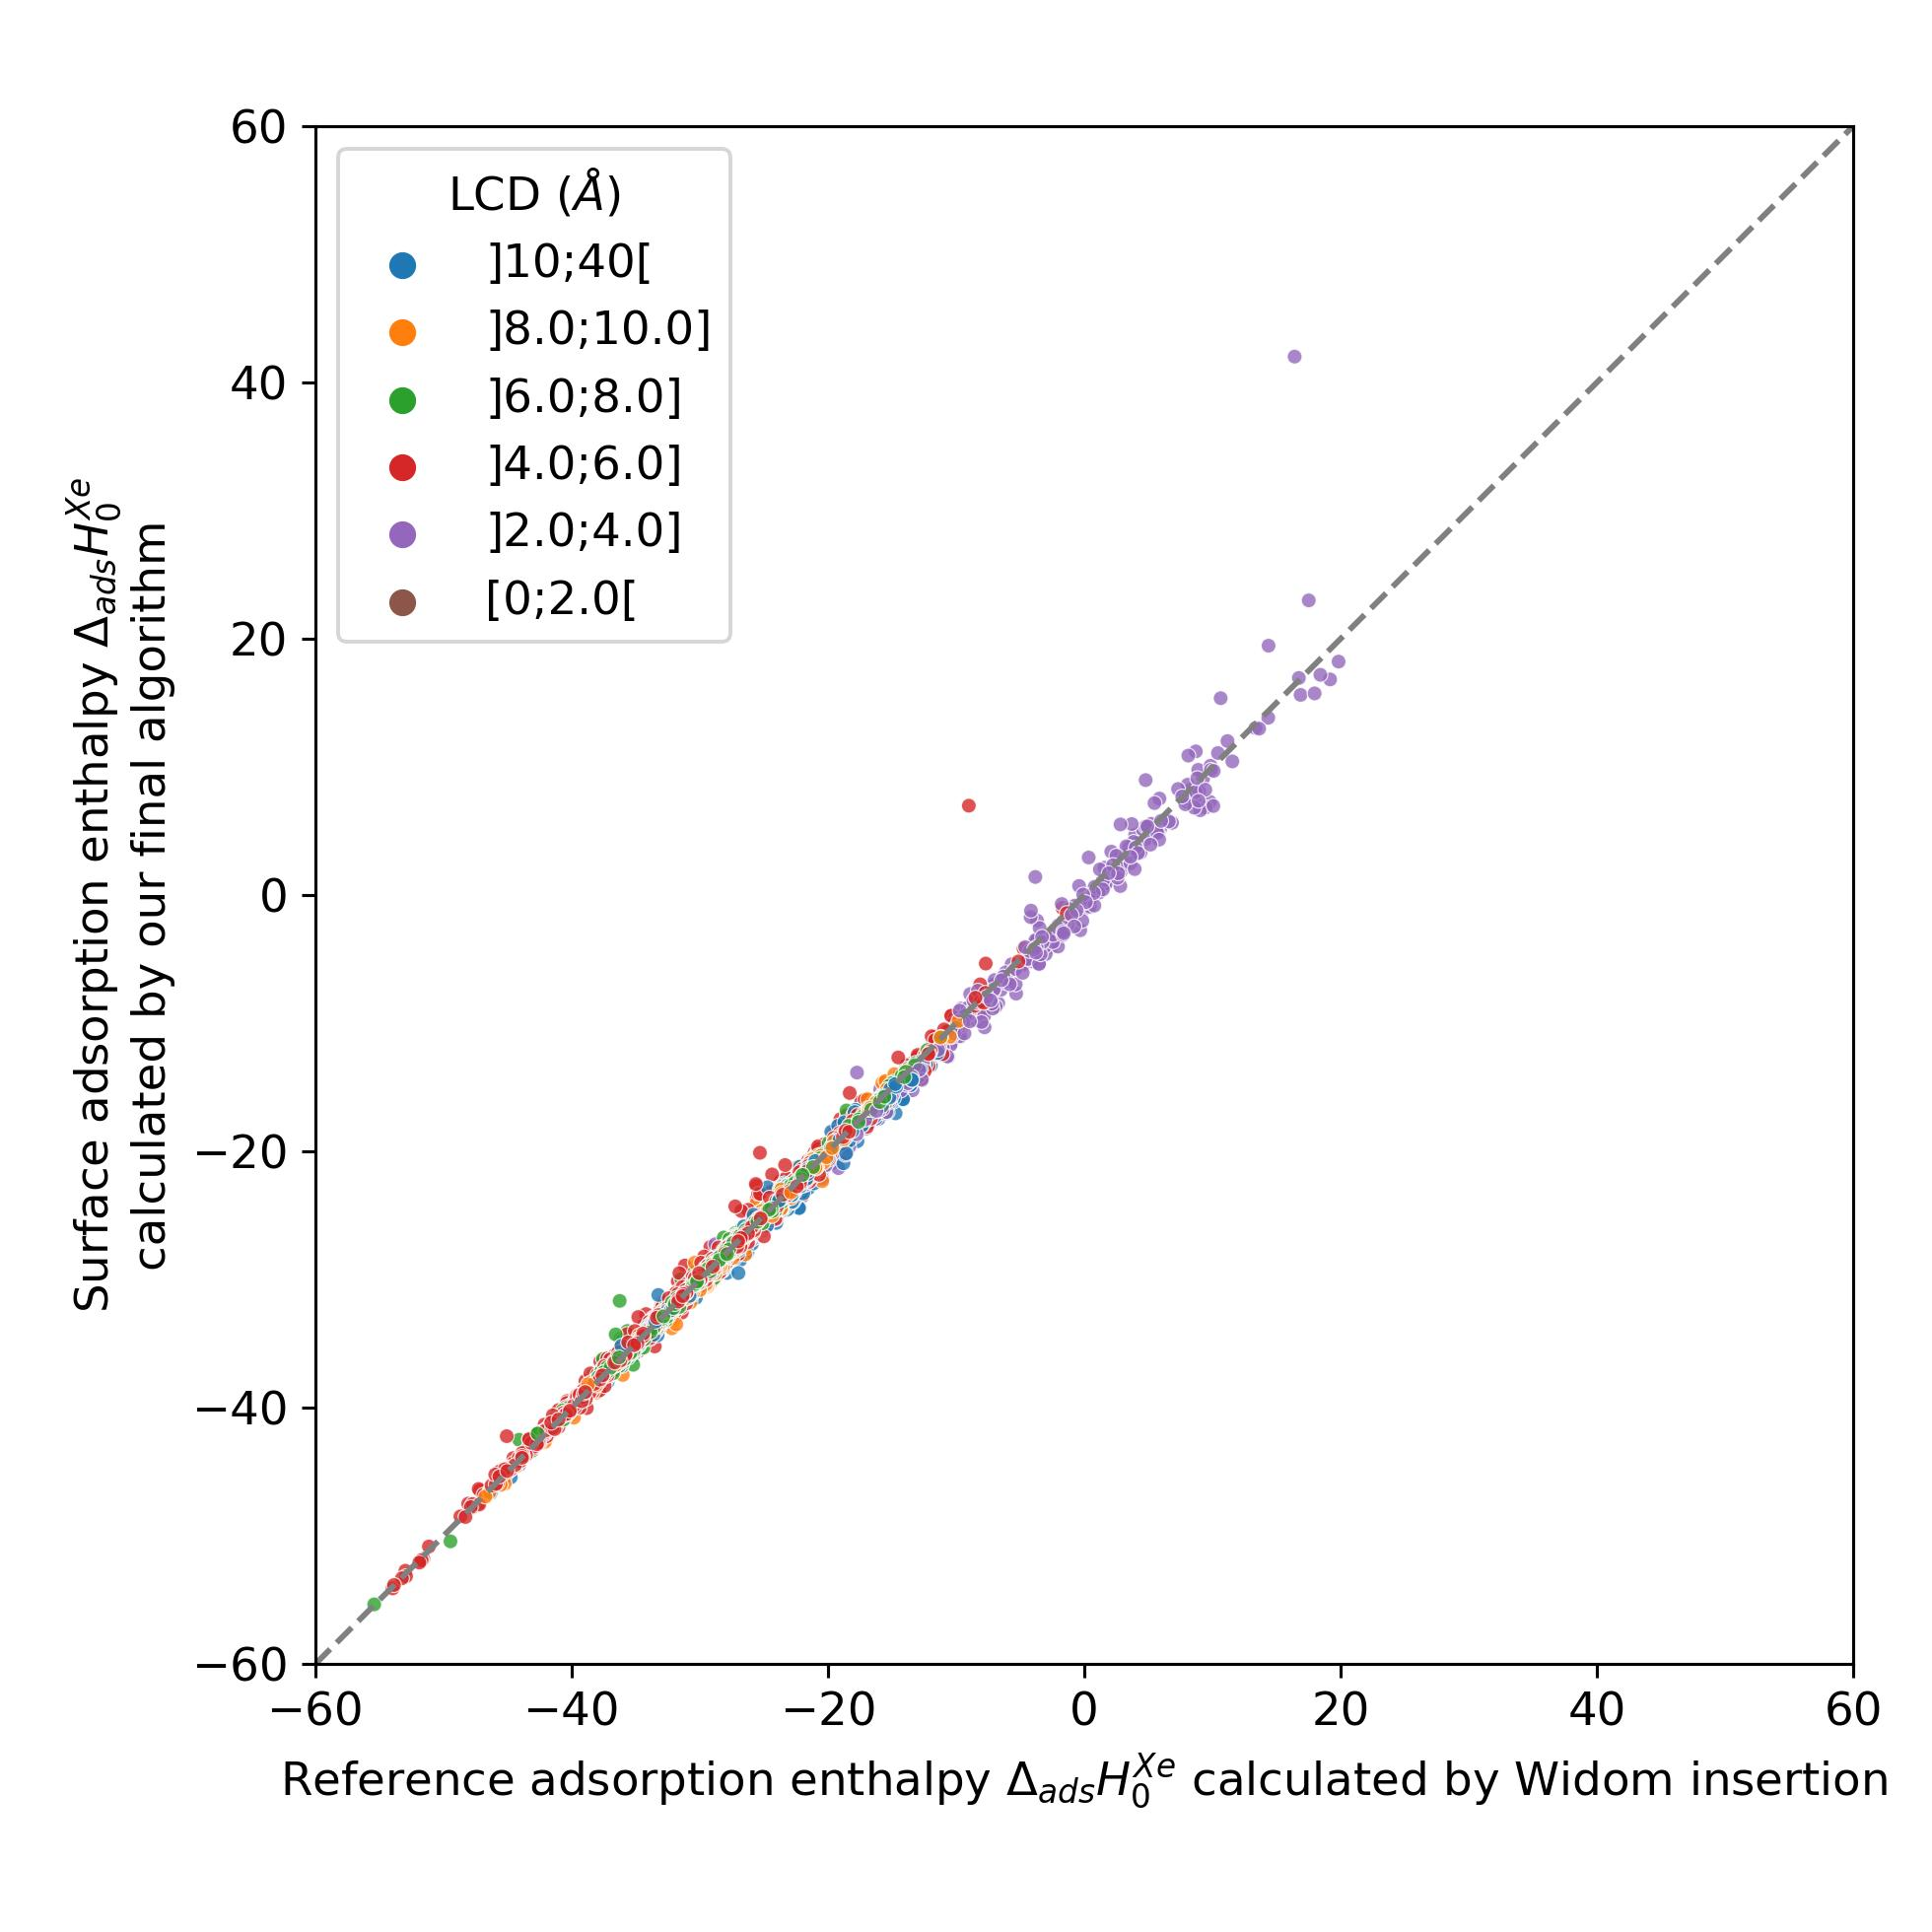
\includegraphics[width=0.45\linewidth]{figures/3-fastsim/H_Xe_widom_vs_H_Xe_surface_final_overview.jpg}
  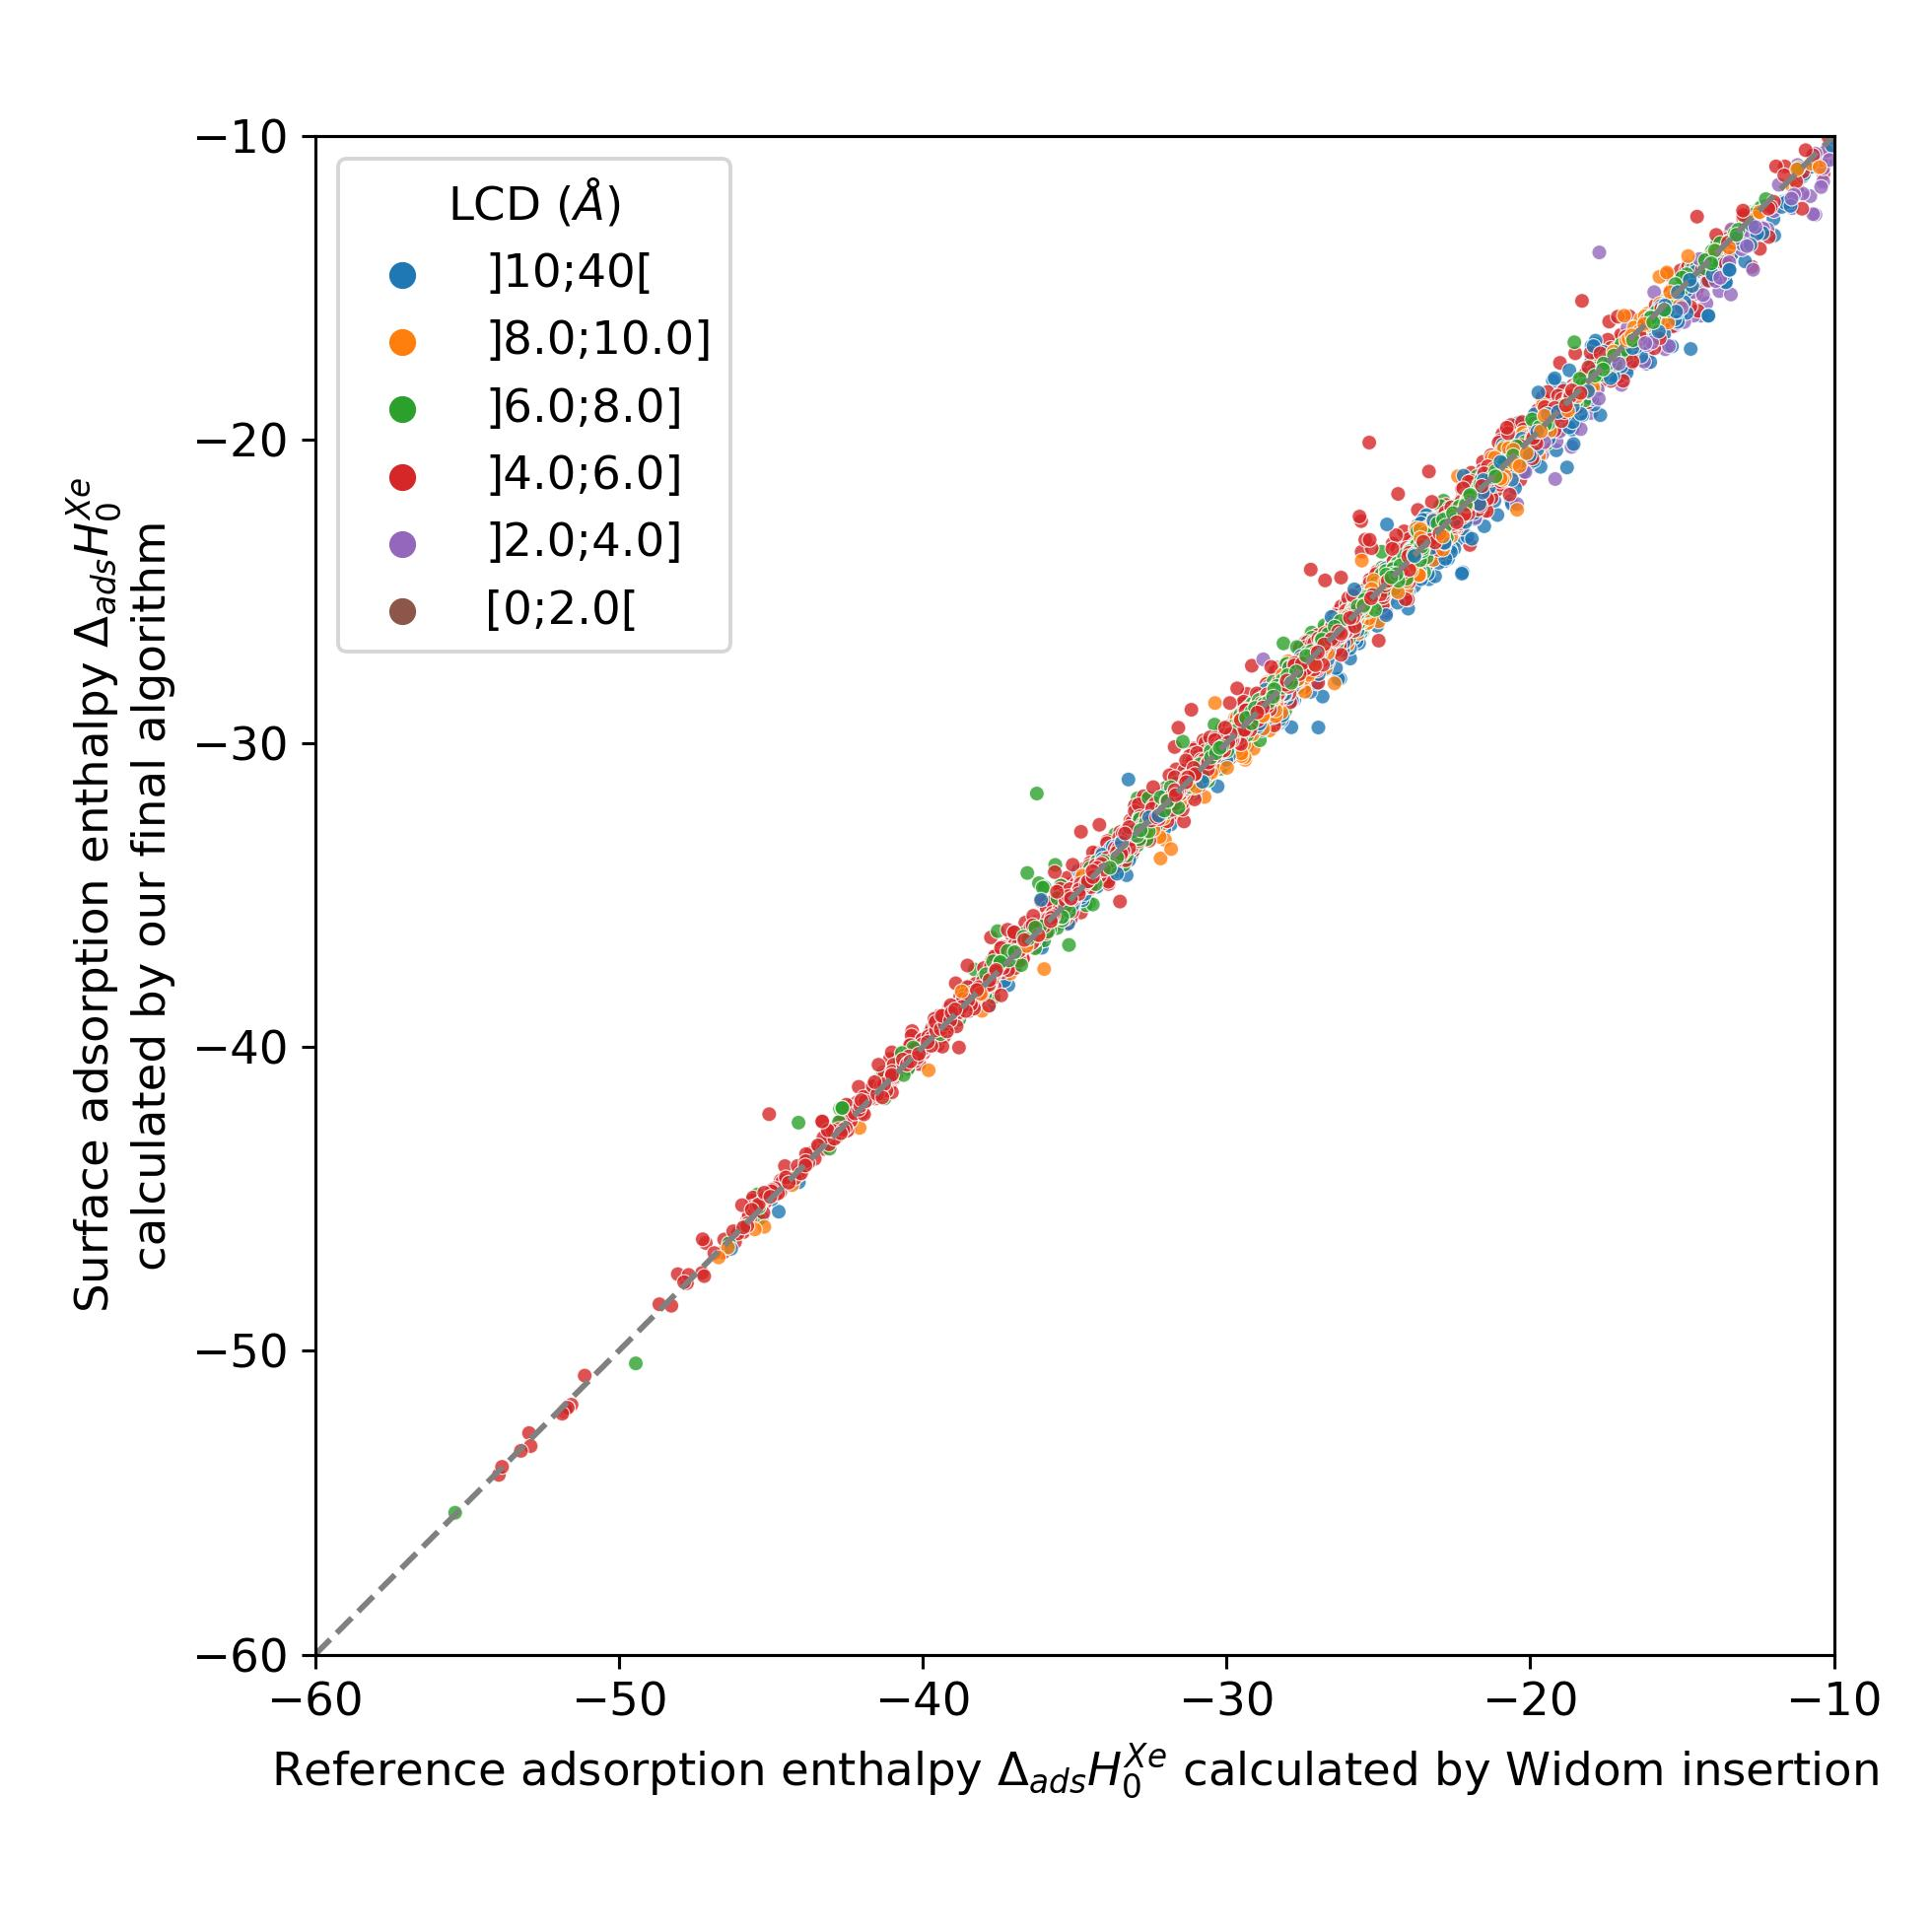
\includegraphics[width=0.45\linewidth]{figures/3-fastsim/H_Xe_widom_vs_H_Xe_surface_final_zoom.jpg}
    \caption{Scatterplots of the xenon surface adsorption enthalpy calculated by the final RAESS algorithm ($\lambda = 1.6$ and $\mu=0.85$) as a function of the xenon adsorption enthalpy calculated by a 100k-step Widom insertion simulation using two value windows, in structures of CoRE MOF 2019 with LCD\e{CCDC} $\geq$ \SI{3.7}{\angstrom} at \SI{298}{\kelvin}. The second plot zooms on the negative values corresponding to the most selective materials.}\label{fgr:surface_sampling}
\end{figure}

% \begin{table}[ht]
%   \centering
%   \begin{tabular}{|l|r|r|}
%   \hline
%                 Method &  RMSE (kJ/mol) &   Time (s) \\
%   \hline
%    surface\_standard\_2k &       0.903953 &   1.045269 \\
%      surface\_radius\_2k &       0.331715 &   1.145985 \\
%   surface\_rejection\_2k &       0.870635 &   0.234415 \\
%       surface\_final\_2k &       0.330454 &   0.339397 \\
%                voronoi &       2.114351 &   0.400000 \\
%              widom\_12k &       0.037631 & 145.058516 \\
%   \hline
%   \end{tabular}
%   \caption{Raw data of the performance of each sampling method}\label{tab:sumup}
% \end{table}

Finally, we suggest that the values of the parameters optimized in this work might need adjustment when applied to other adsorption systems. The optimal $\mu$ parameter depends on the size of the adsorbent, and it should be tweaked differently when considering another adsorbent. For instance, the set of structures used for the optimization of $\mu$ depends on the size of their cavities, and the \SI{3.7}{\angstrom} threshold chosen here would need to be changed according to the kinetic diameter of the adsorbate. Furthermore, as aforementioned in the section on the rejection condition, it is possible to trade off a bit of accuracy for faster simulations especially in high-throughput screenings where speed is extremely important. Similarly, in the case of xenon, the cost of increasing the sphere size is around $10$ to {$20$\%}. On very large databases, one could consider that this increase on the required computational time is not worth the accuracy improvement, and one could decide to keep a smaller sampling sphere. If this method is transposed to different molecular systems, its parameters should be tested on the specific database and adsorbate of interest.

\begin{figure}[ht]
  \centering
    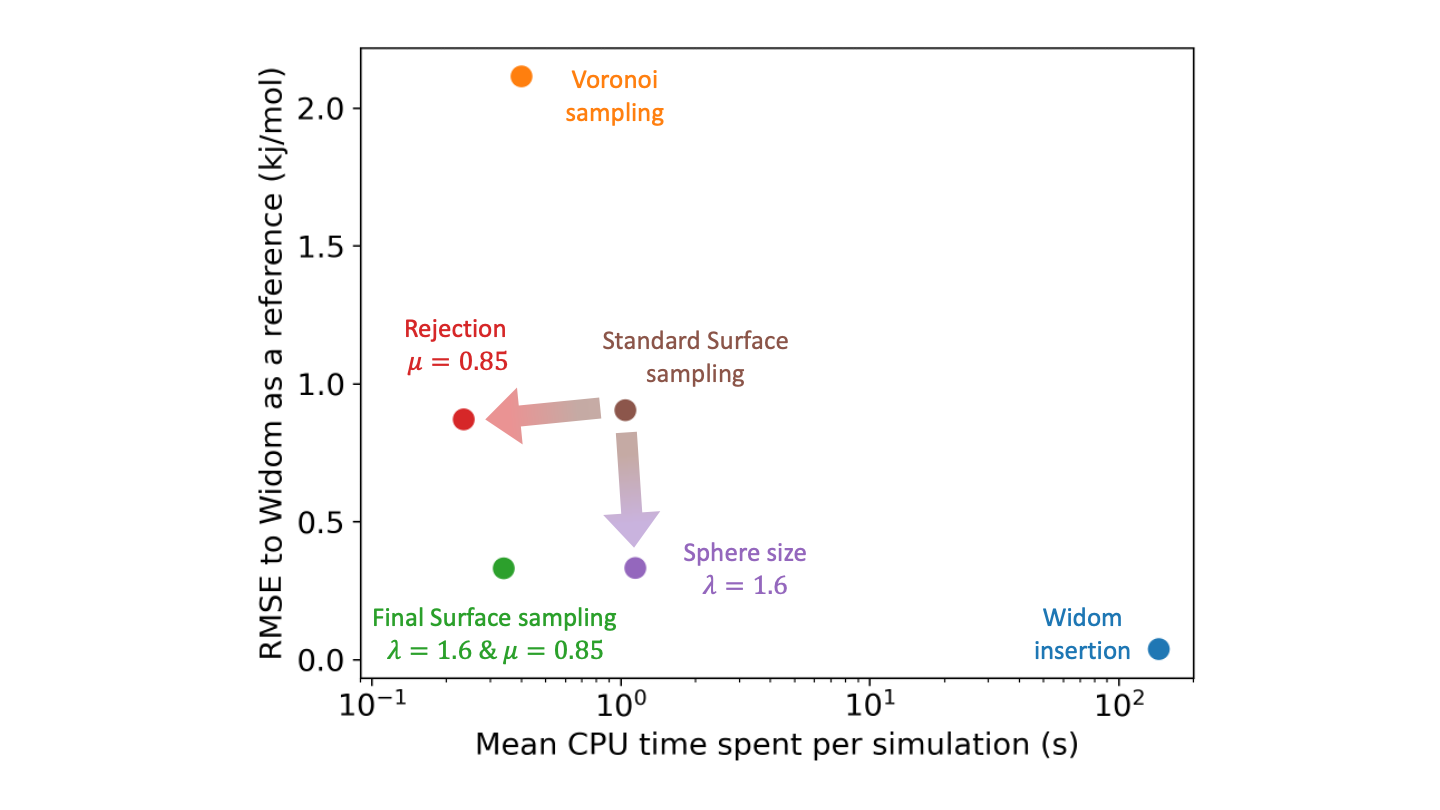
\includegraphics[width=\linewidth]{figures/3-fastsim/methods_comparison.png}
    \caption{Comparison of the RMSE to the reference Widom insertion and the average computation time for different types of enthalpy calculation methods. The surface sampling calculation were all done with 2k sampling points on each sphere and the Widom simulations were done using 12k cycles. These values correspond to the value at the convergence identified using Figure~\ref{fgr:convergence}. }\label{fgr:sumup}
  \end{figure}

\subsubsection{Calculation of Henry constant and surface area}

The main goal of our sampling algorithm is to calculate adsorption enthalpy in the zero-loading limit. But the method can also calculate at the same time the Henry constant and surface area of the materials, without significant additional computational cost. The Henry constant is a key metric for assessing the affinity of an adsorbate to a nanoporous structure. The Xe/Kr gas selectivity at low pressure is defined as a ratio of Henry constants of Xe and Kr. This important property can be calculated using Equation~\ref{eq:eq_cst} in a Widom insertion calculation. Instead of using the interaction energies at the Widom inserted points, we can now use the surface sampled points to get an approximate value for the Henry constant.

\begin{figure}[ht]
  \centering
  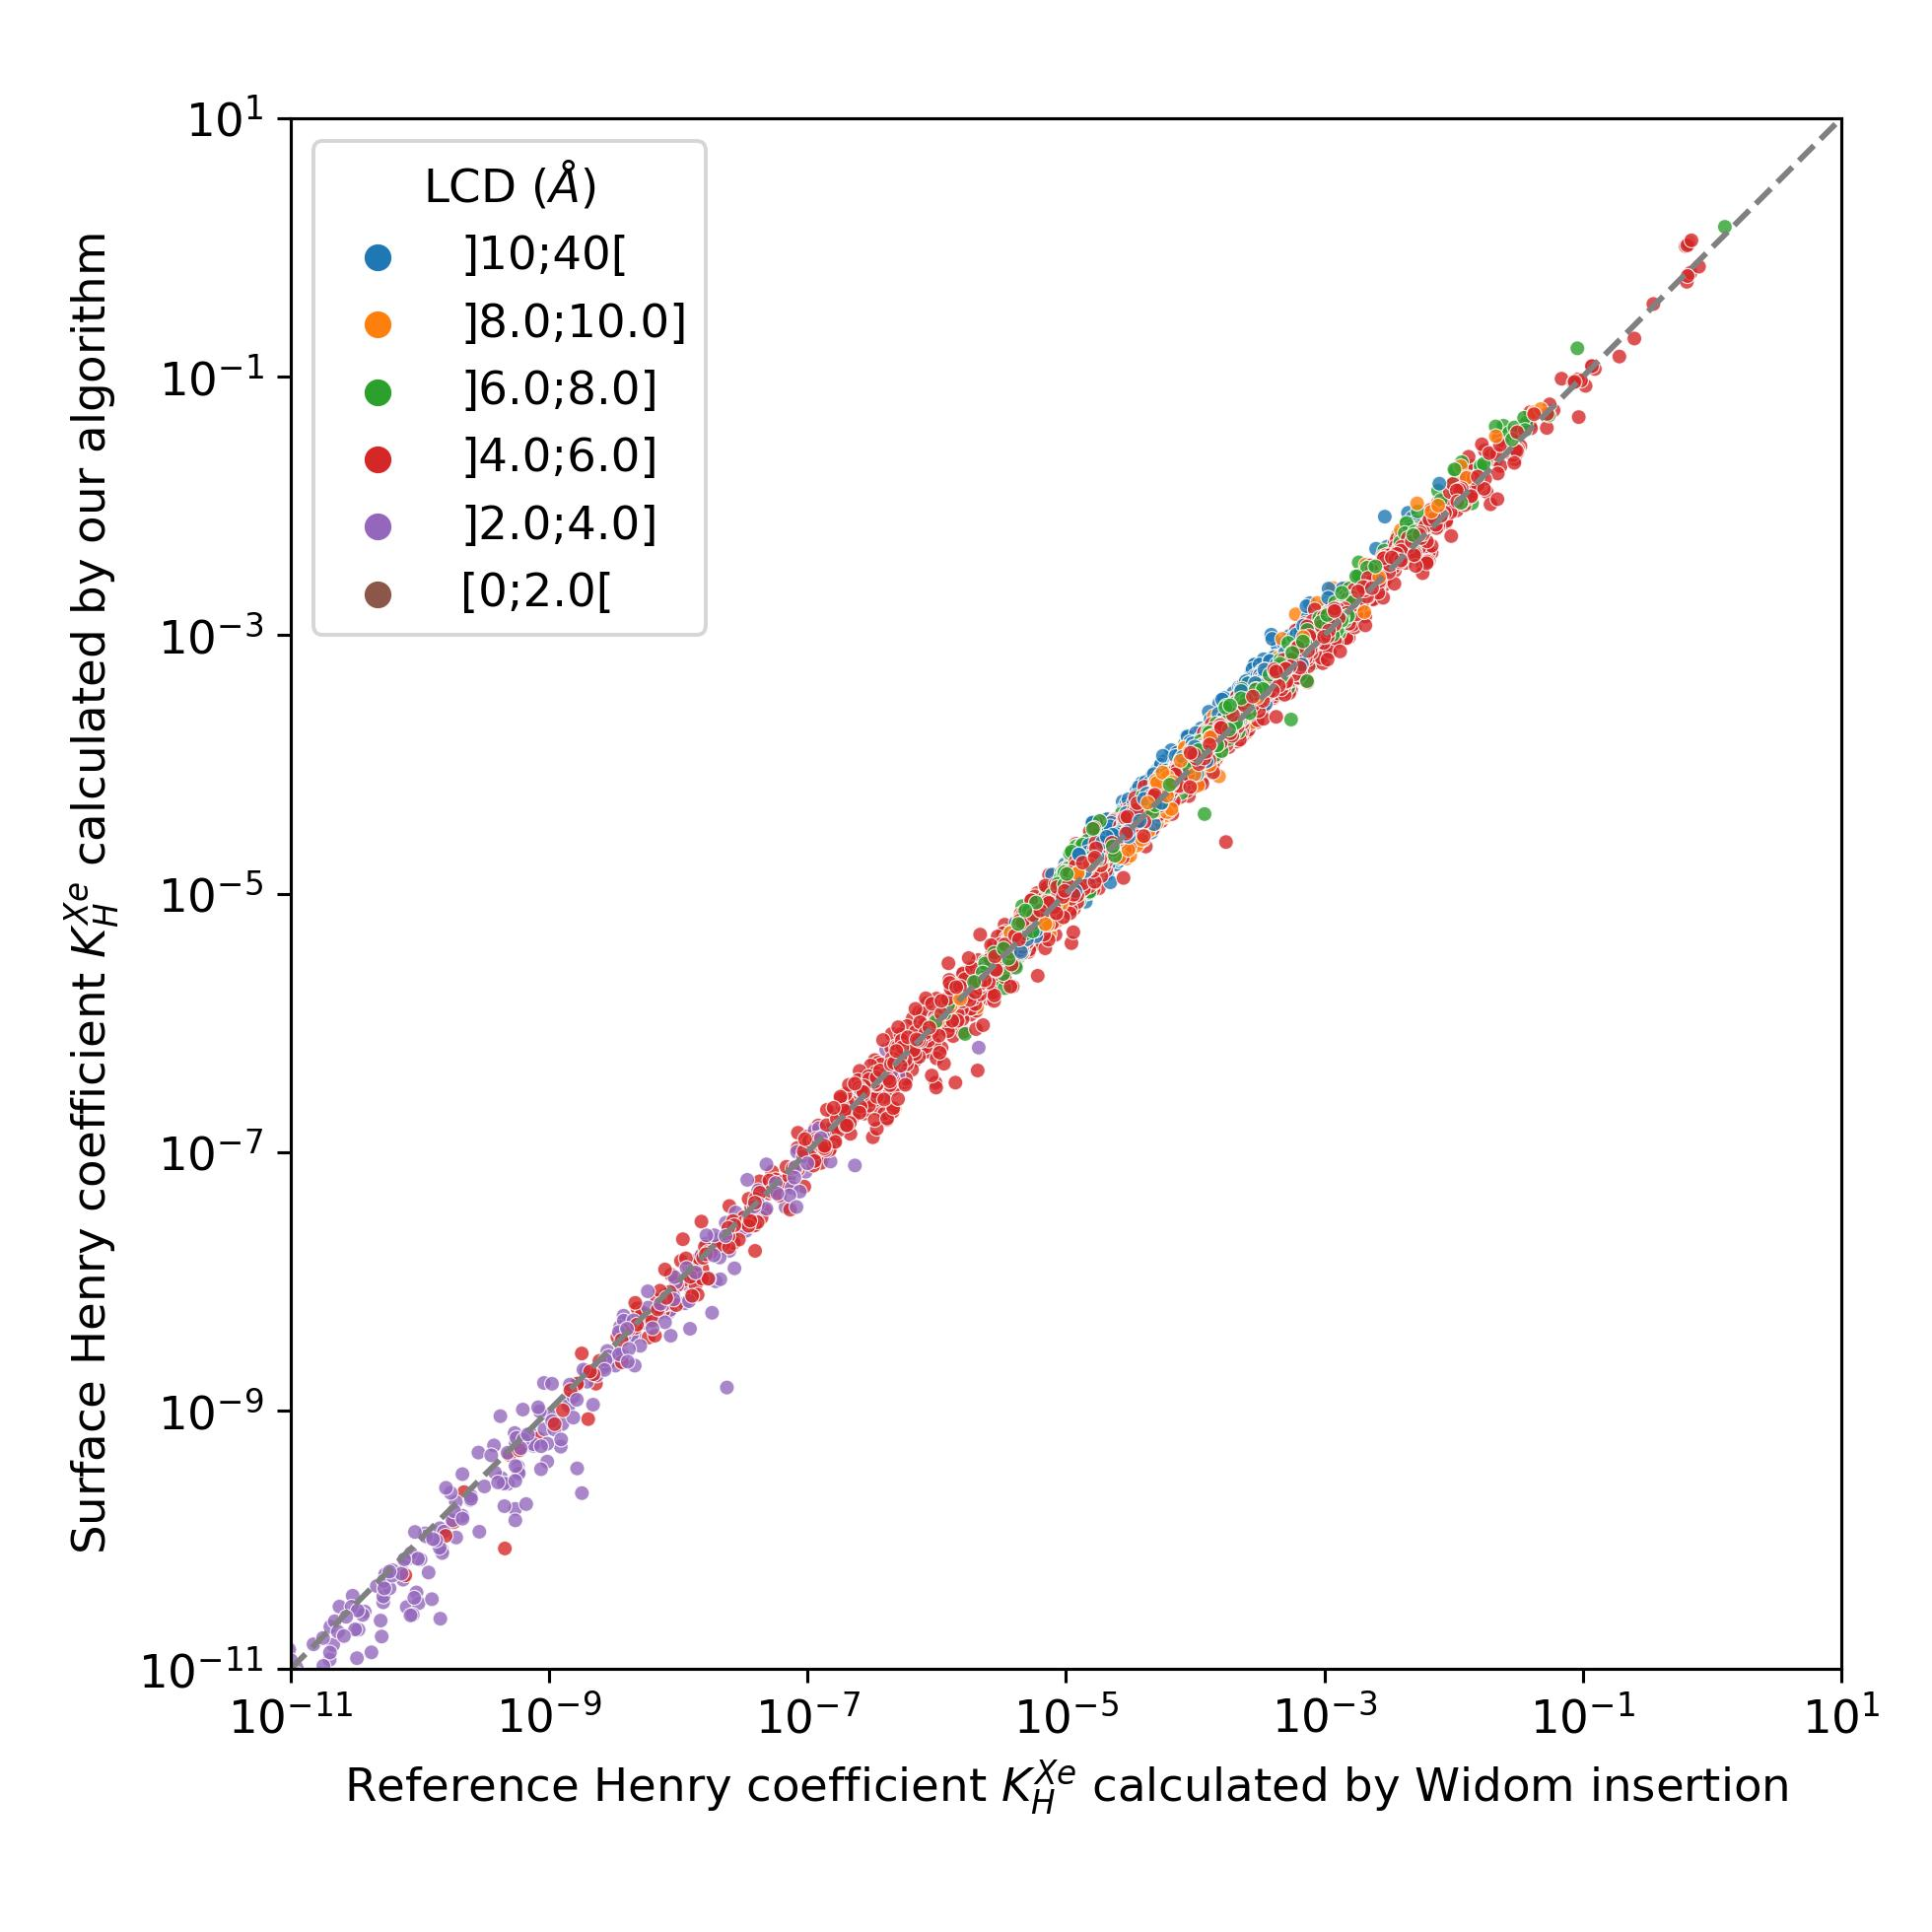
\includegraphics[width=0.6\linewidth]{figures/3-fastsim/K_Xe_widom_vs_K_Xe_surface_final_zoom.jpg}
    \caption{Scatterplots of the xenon Henry constants calculated by the RAESS algorithm compared to the ones calculated by a 100k-step Widom insertion simulation using two value windows.}\label{fgr:henry_scatter}
\end{figure}

Using the optimized set of parameters for surface sampling, we assessed the performance of our algorithm on the values of Henry constant by comparing them to ground truth obtained by 100,000 cycles of Widom insertion. Since the Henry constant corresponds to the exponential of an adsorption free energy, and we are more interested in the precision on the free energy, we are using a log-scale evaluation metric. For surface sampling, the log-RMSE of $K\e{H}$ is equal to $0.2$, which means that the order of magnitude of the values are well predicted as we can see on the Figure~\ref{fgr:convergence_free_energy}. If we consider the derived free energy $\Delta F_{ads} = -RT \log(\rho_fRT K_H)$, the RMSE is of the order of \SI{1.1}{\kilo\joule\per\mole} reached in about \SI{1}{\second} (Figure~\ref{fgr:convergence_free_energy}). Whereas for Widom insertion, this level of error is also reached in a similar amount of time and \SI{0.1}{\kilo\joule\per\mole} of RMSE is reached in about \SI{86}{\second} (Figure~\ref{fgr:convergence_free_energy}). For free energy calculation, surface sampling is still 86 times faster to converge. If consider that the main target is the adsorption enthalpy, the Henry constant is calculated with little additional computational cost and with reasonable accuracy: we get two thermodynamic properties of interest for the price of one.

\begin{figure}[ht]
  \centering
  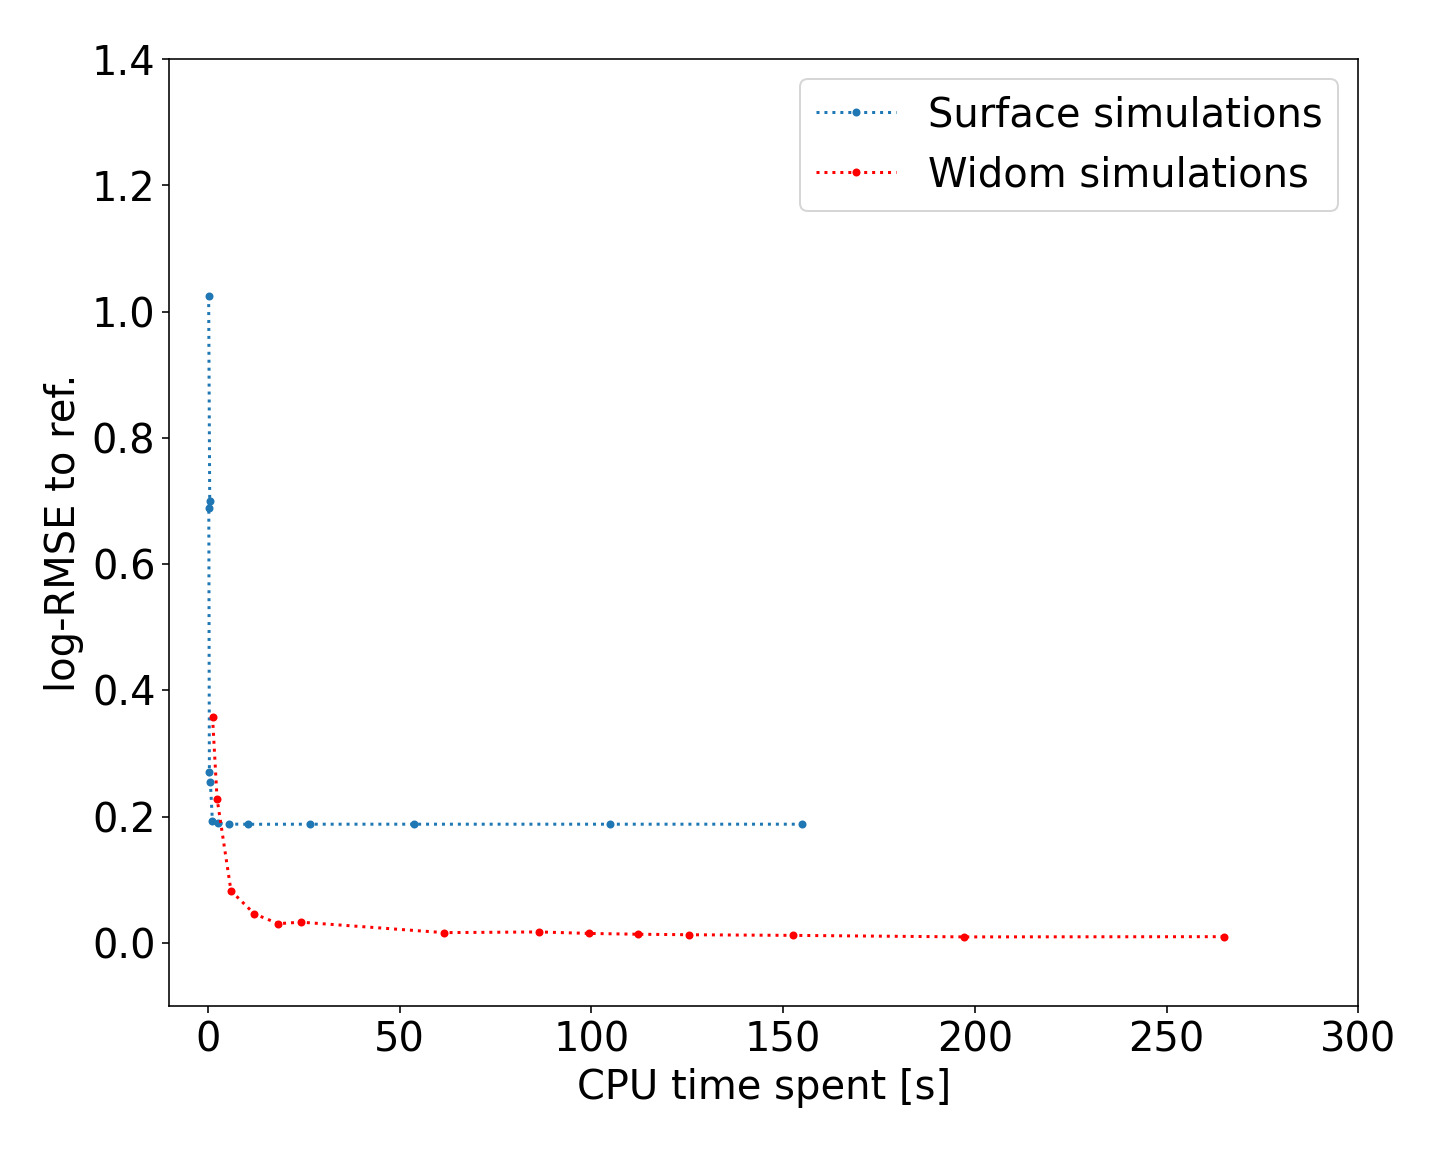
\includegraphics[width=0.45\textwidth]{figures/3-fastsim/log_henry_convergence.jpg}
  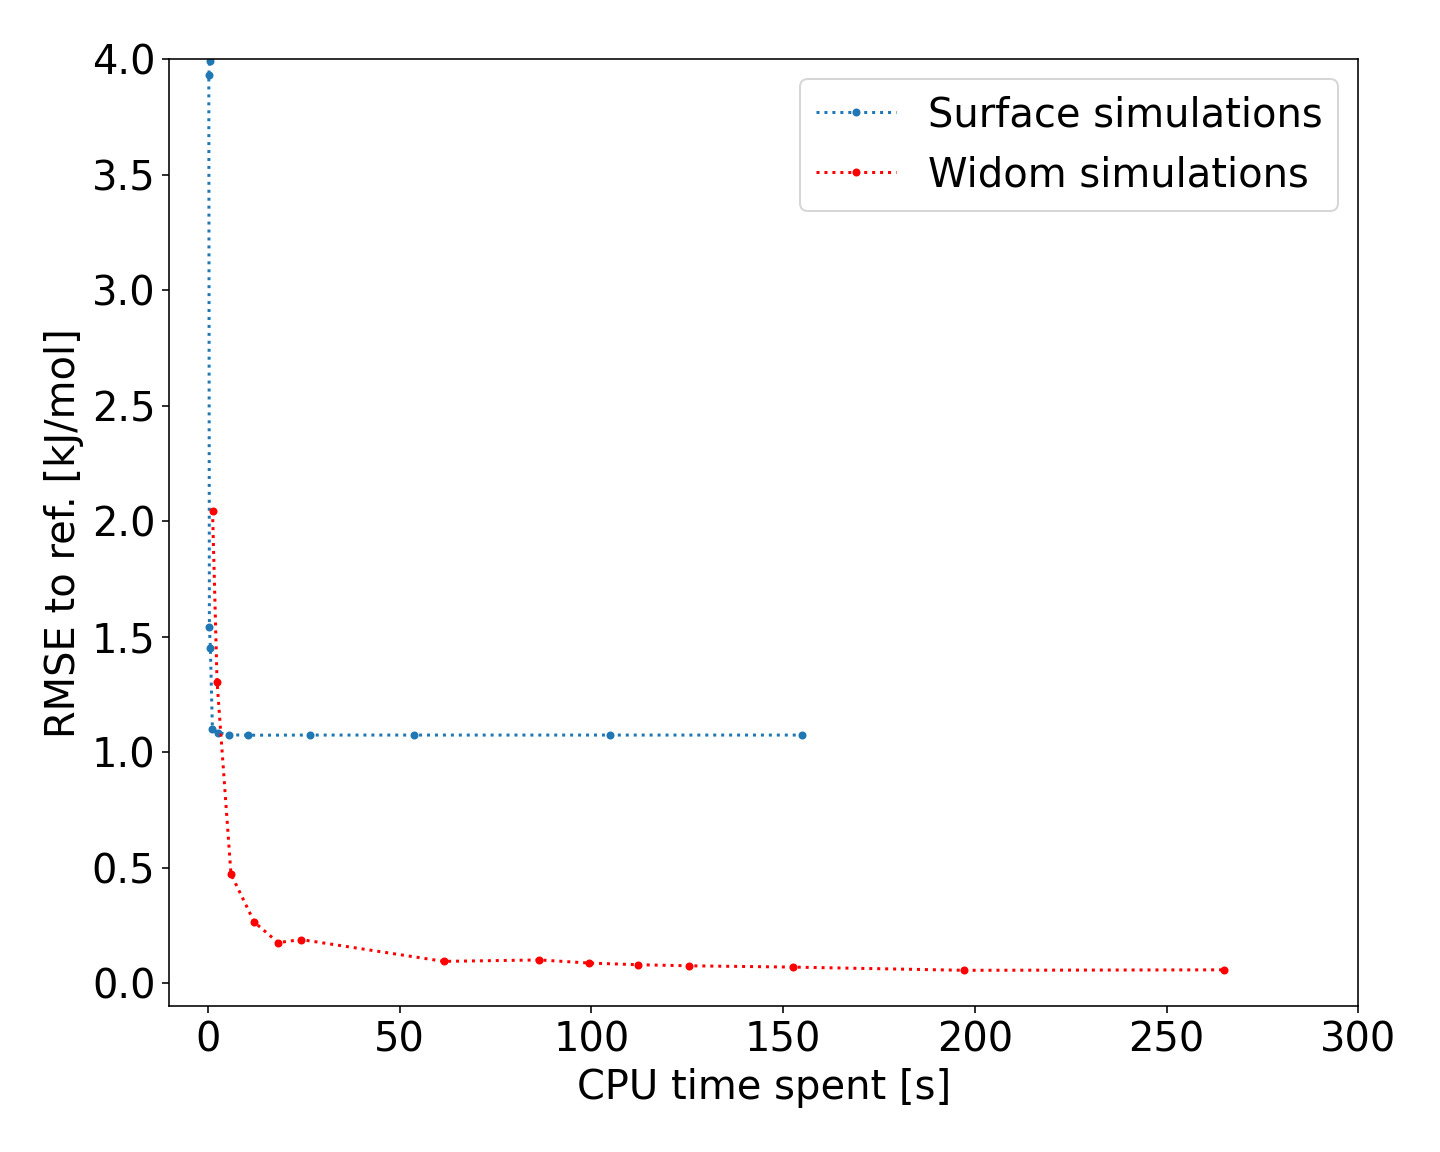
\includegraphics[width=0.45\textwidth]{figures/3-fastsim/gibbs_free_energy_convergence.jpg}
  \caption{ Left: convergence plot of the log-RMSE on the xenon Henry constants for both the surface sampling and the Widom insertion. Right: convergence plot of the RMSE on the xenon adsorption Gibbs free energy for the final implementation of the surface sampling and the Widom insertion. }\label{fgr:convergence_free_energy}
\end{figure}

The same goes for the determination of the surface area. We can adapt our algorithm to count the number of points of the sampling spheres that have a negative energy. These represent the points were a guest molecule can favorably interact, therefore when dividing it by the number of sampled points, we obtain a proportion of adsorbable area of the sphere. Summing this over all atoms, we obtain a total surface area. This implementation is summed up in equation~\ref{eq:sa}:
\begin{equation}
\label{eq:sa}
    \textrm{SA} = \dfrac{1}{V}\sum_{a\in \textrm{cell}} \dfrac{N\e{accessible}(a)}{N\e{total}}4\pi {r(a)}^2
\end{equation}
where $V$ volume of the cell $a$ atoms of the cell; $N_{accessible}(a)$ accessible points around the atom $a$; $N_{total}$ sampling points; $r(a)$ radius of the sampling sphere around the atom $a$.
When we set $\lambda=1$, we are sampling spheres that have a radius $\sigma$, and it is equivalent as considering hard spheres all defined by $\sigma$ (convention used by RASPA2 to calculate surface areas). If we compare simulation with $\lambda=1$, we obtain surface areas that are very close to the one obtained by RASPA2 (see Figure~\ref{fgr:surface_area} in SI). However, when we consider $\lambda=1.6$, we lose the perfect accordance previously obtained and the points weakly correlated in log-scale (see Figure~\ref{fgr:surface_area} in SI). The difference can be explained by the fact that the sphere size is larger, but the proportion of adsorbable points also changes. The relationship between these two adsorption surface areas is not trivial at all. Since the calculation of surface areas is quite cheap, this implementation would not be very useful, except for having a rough idea of the surface area.

\begin{figure}[ht]
  \centering
  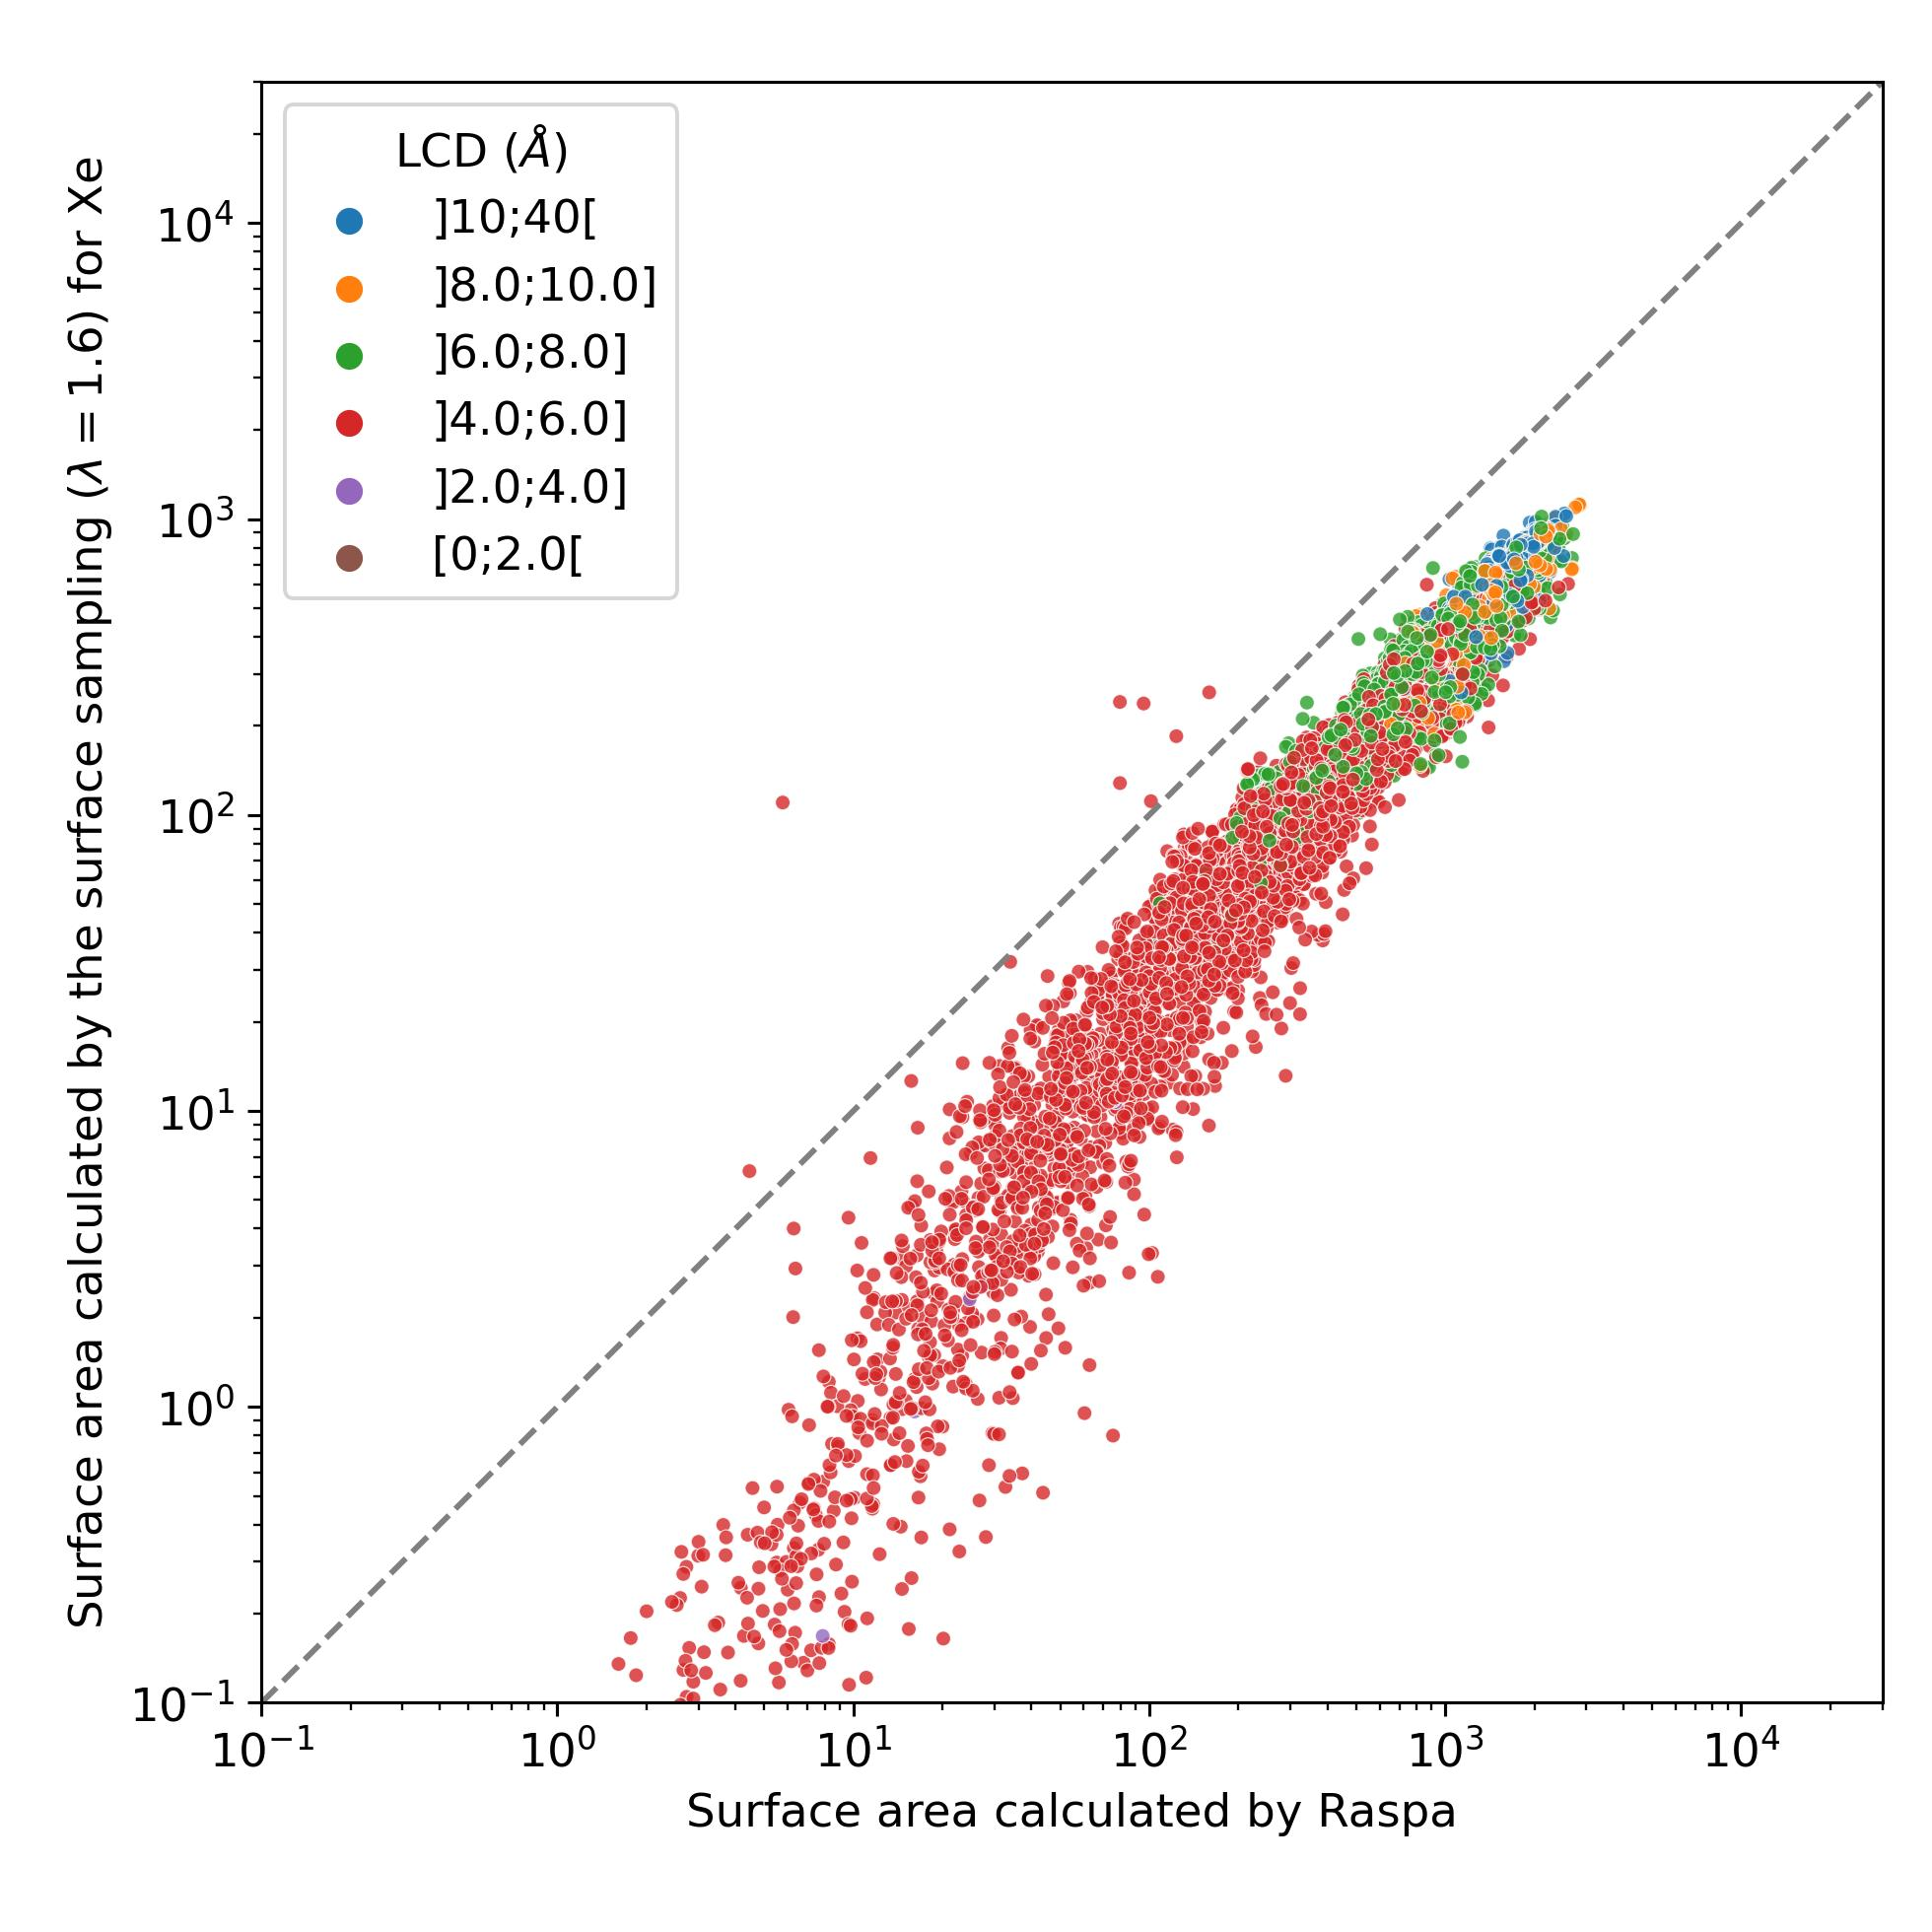
\includegraphics[width=0.45\textwidth]{figures/3-fastsim/SA_raspa_Xe_m3_cm3_vs_SA_lambda_1.6_overview.jpg}
  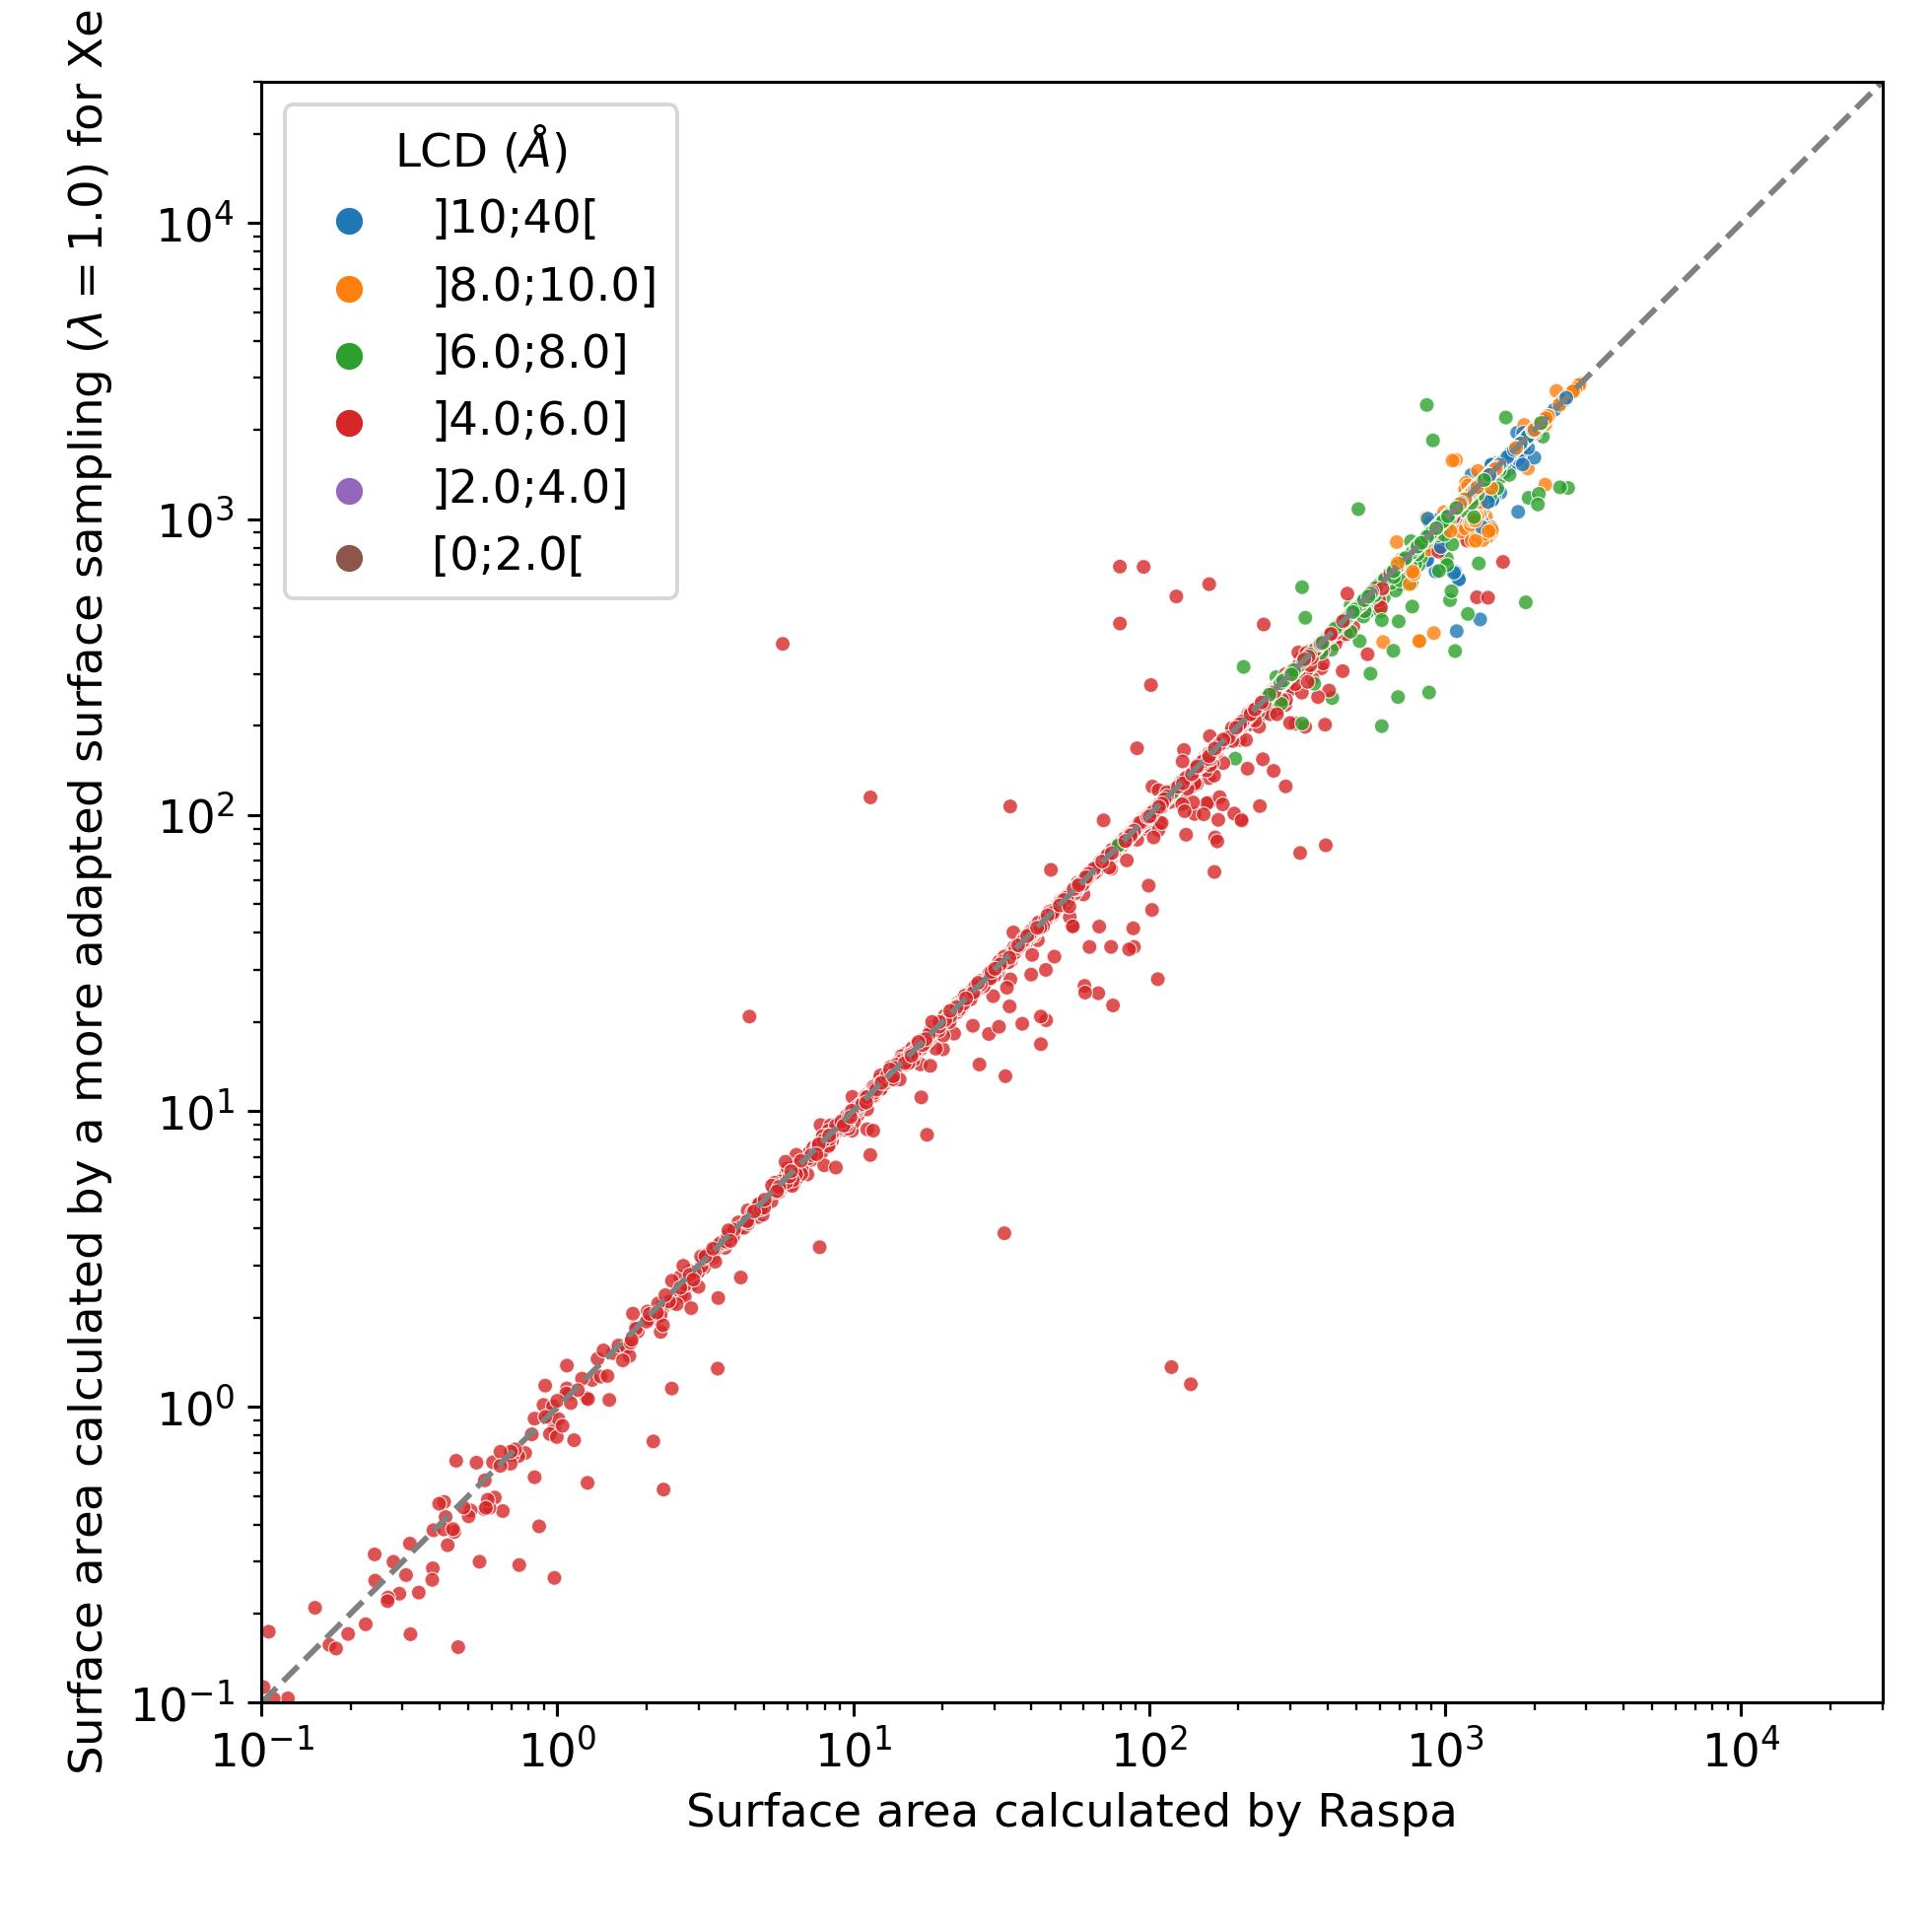
\includegraphics[width=0.45\textwidth]{figures/3-fastsim/SA_raspa_Xe_m3_cm3_vs_SA_lambda_1.0_overview.jpg}
  \caption{Scatterplots of the surface areas calculated by our algorithm with two different parameterizations compared to the surface area given by a Raspa surface area calculation. The left plot corresponds to the surface sampling described in the section~\ref{sct:final_sampling} with $\lambda=1.6$ and $\mu=0.85$, while the right plot uses a sampling sphere near $\sigma$ with $\lambda=1.0$. The second parameterization is much closer to what a Raspa sampling based on the $\sigma$ parameter of a LJ potential does, hence explaining the much better accordance. }\label{fgr:surface_area}
\end{figure}

\subsection{Surface sampling application use cases}

After introducing the performance of our surface energy sampling algorithm for xenon and on specific materials from CoRE MOF 2019 at \SI{298}{\kelvin}, we will explore other conditions to test the transferability of the methodology. First, we will use the algorithm to assess the xenon/krypton selectivity at infinite dilution  compared to the standard Widom insertion. Then, we want to compare the influence of the temperature on the performance since it most likely would be much less ideal since the Boltzmann weights are less concentrated on the less attractive points. Finally, we tested our algorithm on databases of different materials. 

\subsubsection{Selectivity Calculations}

The selectivity value is the most important metric in evaluating the Xe/Kr separation performance of a nanoporous material. We want to see if a surface sampling technique can accurately evaluate this metric while being limited by all the approximations inherent to the technique.

A few precautions should be considered before blindly using the algorithm for selectivity prediction. When investigating the calculation of the selectivity, we noted that the rejection condition on xenon can be high since we are interested in the most favorable materials for xenon adsorption. But for krypton, we want to accurately describe very low Henry constants, because a selective material would also be a material unfavorable to krypton. For these reasons, the parameter $\mu$ needs to be chosen wisely and needs to be low enough to have accurate Kr Henry constant and then selectivity values. 

As we can see on the Table~\ref{tab:selec_prob}, the error on the selectivity highly depends on the $\mu$ value that excludes the points at $\mu\sigma$ of a framework atom center. Logically, the lower this parameter the higher the sampled energy values can be in the Boltzmann averaging. Another reason is that when dividing by small values any small error on the values can be amplified in the quotient, and this effect can be reduced as we increase the number of points actually sampled. 

\begin{table}[ht]
  \centering
  \begin{tabular}{|l|r|r|}
  \hline
    rejection parameter $\mu$ &  log10-RMSE to 100k-Widom &   log10-MAE to 100k-step Widom \\
  \hline
      0.85 &      0.107 &   0.077 \\
      \textcolor{red}{0.50} &      \textcolor{red}{0.0635} &   \textcolor{red}{0.0402} \\
      0.20 &      0.0637 &   0.0403 \\
  \hline
  \end{tabular}
  \caption{Influence of the rejection condition in the krypton surface simulation on the accuracy of the Xe/Kr selectivity calculation. The lower the parameter $\mu$ the more accurate the simulations are for the final selectivity calculation.}\label{tab:selec_prob}
\end{table}

According to the quick study here, the optimal value is $\mu=0.5$ since it gives the best accuracy for a minimal amount of time. This value will be used for krypton to make a comprehensive study of the performance on the Xe/Kr selectivity for materials from CoRE MOF 2019. To sum up, in the following study, we will use the RAESS algorithm with $\lambda=1.6$ and $\mu=0.85$ for xenon and $\lambda=1.6$ and $\mu=0.5$ for krypton.

The selectivity can be compared directly using a log-scale plot and log-scale metrics. If we apply the log10 to the selectivity values, we obtain RMSE of 0.064 and MAE of 0.04. This means that we have an error of about 0.06 when we compare orders of magnitude of the selectivity. For example, if a selectivity is predicted to be $s = 10^{-7}$, then $s$ would be in the interval $[10^{-7.06},10^{-6.94}]$.

\begin{figure}[ht]
\centering
  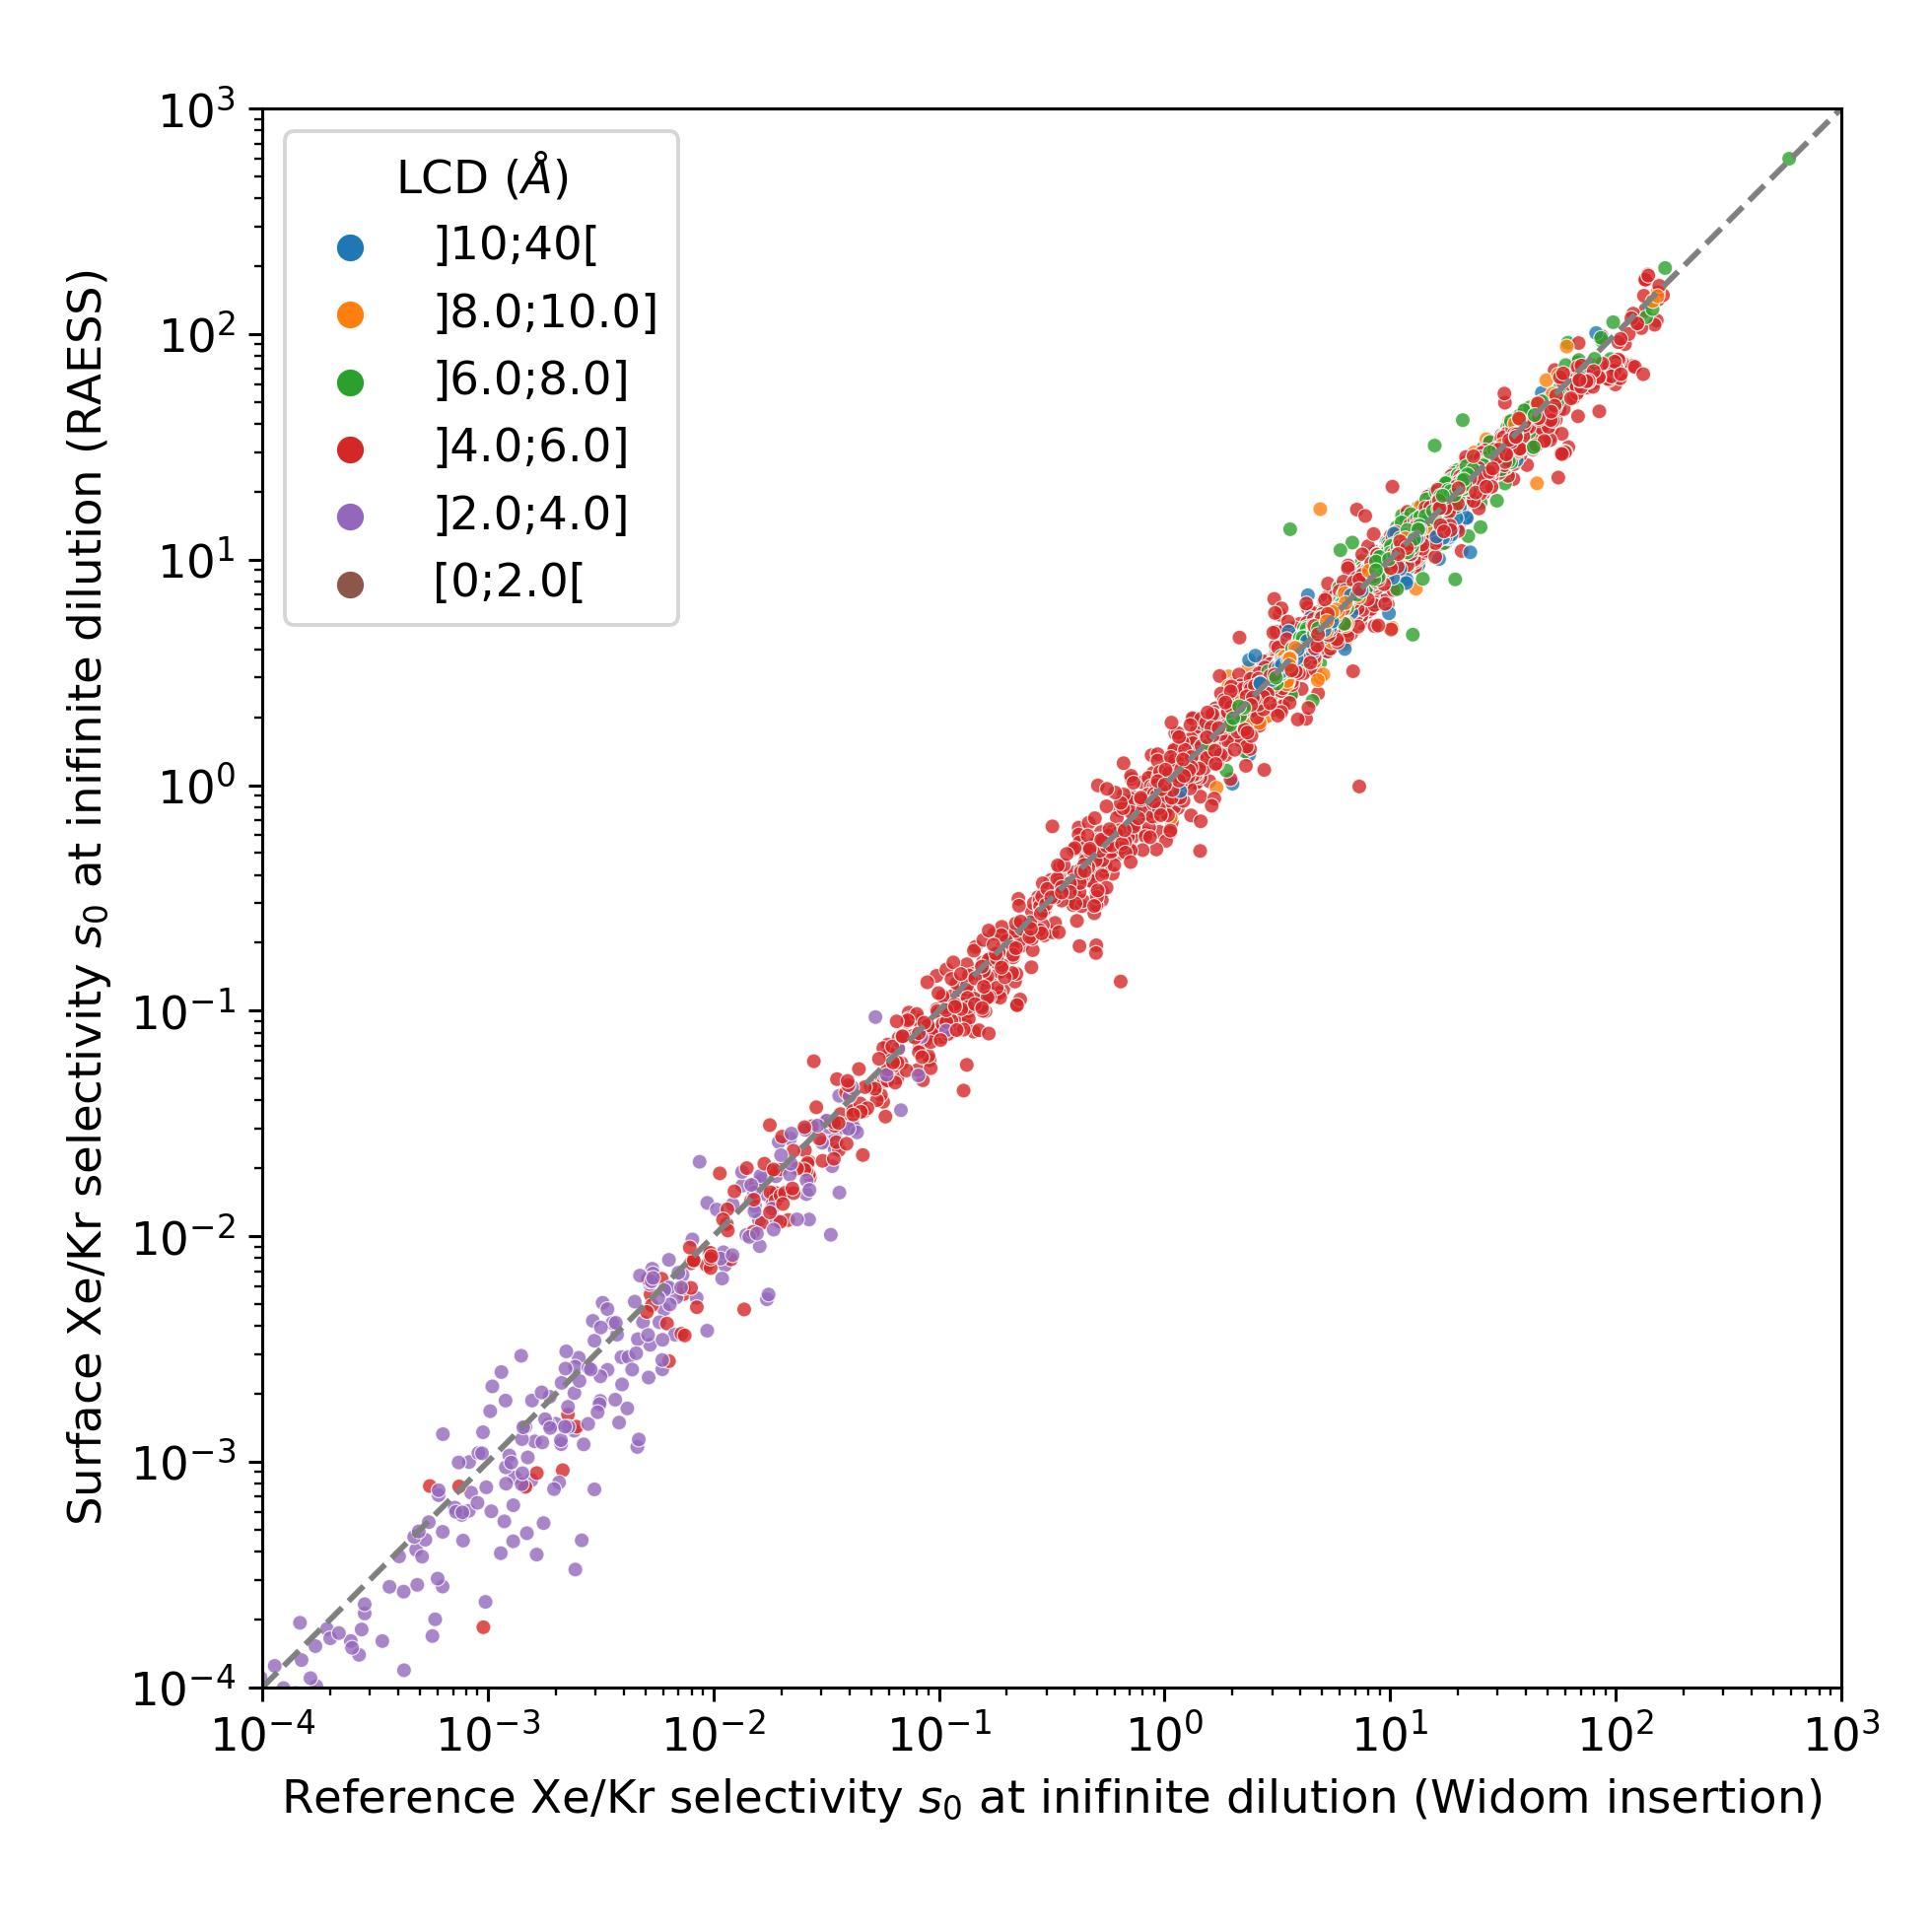
\includegraphics[width=0.5\linewidth]{figures/3-fastsim/s_0_widom_vs_s_0_surface_zoom.jpg}
  \caption{Scatterplot comparison of the Xe/Kr selectivity calculated by RAESS algorithm and the one calculated by the Widom insertion (in log scale) and labeled by the cavity size. }\label{fgr:s_0}
\end{figure}

To be able to give a thermodynamic interpretation, we can use the exchange Gibbs free energy associated $\Delta\e{exch}G\e{0}\ex{Xe/Kr}$ to this selectivity defined in the previous chapter (equation~\ref{eq:exc_gibbs_free_energy}). Using this exchange Gibbs free energy, we can assess much more easily the performance of the approach. The RMSE is about \SI{0.36}{\kilo\joule\per\mole}. We cannot compare it to the adsorption enthalpy errors, since the ranges and interpretation are very different. Here, the selective materials have a negative $\Delta\e{exch}G\e{0}\ex{Xe/Kr}$, and it goes to a maximum value of about \SI{-12.7}{\kilo\joule\per\mole}. The relative error is, of course, higher on the Gibbs free energy. This is due to a higher uncertainty on the Henry constant and to the denominator term brought by the krypton.

\begin{figure}[ht]
\centering
  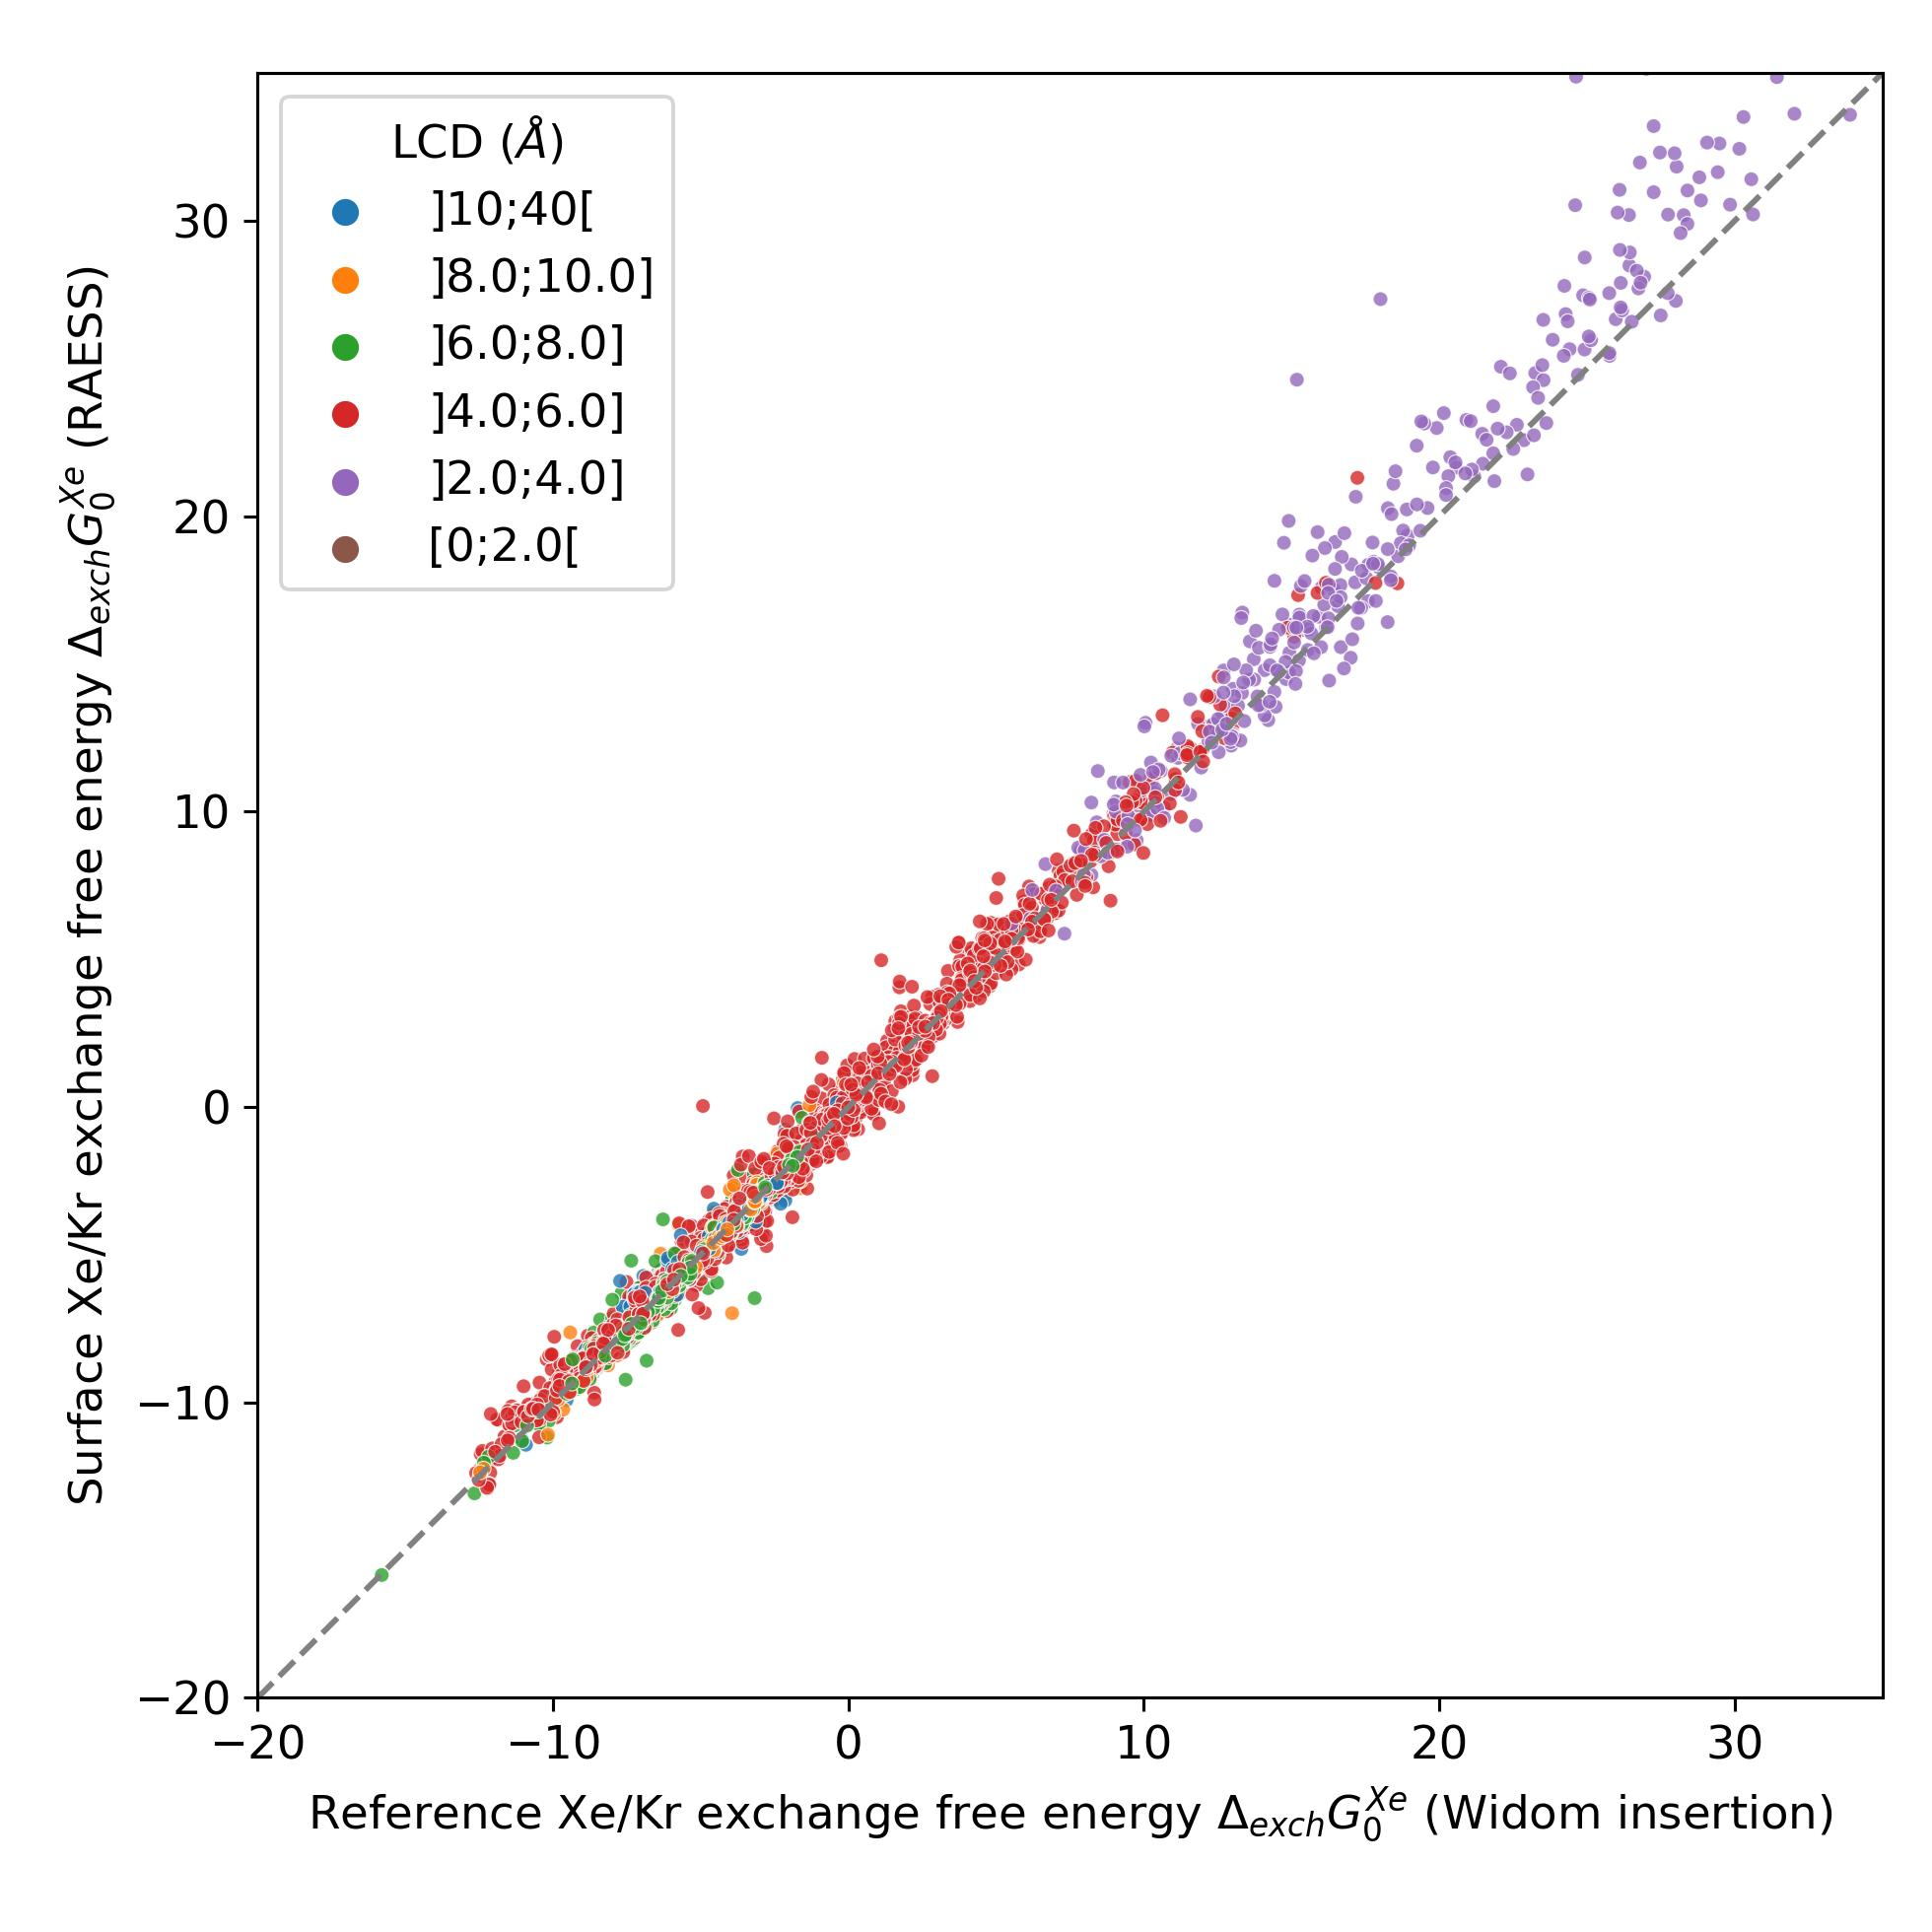
\includegraphics[width=0.5\linewidth]{figures/3-fastsim/G_XeKr_widom_vs_G_XeKr_surface_zoom.jpg}
  \caption{Scatterplot comparison of the exchange Gibbs free energy $\Delta\e{exch}G\e{0}\ex{Xe/Kr}$ calculated by the Widom insertion compared to the final implementation of RAESS (RMSE=\SI{0.36}{\kilo\joule\per\mole} and MAE=\SI{0.23}{\kilo\joule\per\mole}).}\label{fgr:exch_free_energy}
\end{figure}

To know how well the RAESS algorithm would work in real situations, we tried to compare the top 100 most selective materials given by RAESS and a Widom simulation (RASPA2). We found that 83 structures of the top 100 given by RAESS are in the top 100 given by Widom insertion. As the correlation is not perfect, it is inevitable that there is a change in the order of the top 100 given by these two methods. This number of {83\%} proves that the difference is quite narrow. If we enlarge to the top 150 of the Widom simulation, 94 are present in the top 100 of the surface simulation. We can therefore say that a vast majority of the best candidates given by the Widom insertion simulation are found by the RAESS algorithm.


\subsubsection{A Higher Temperature}

The RAESS method relies on the higher weight of the strong sites close to the surface of the pores. If we increase the temperature, the less attractive sites would play an increasing role and the accuracy of the method would drop. To grasp this limitation of the RAESS algorithm at higher temperature, we compared the results of a screening over the CoREMOF 2019 database.  

\begin{figure}[ht]
\centering
  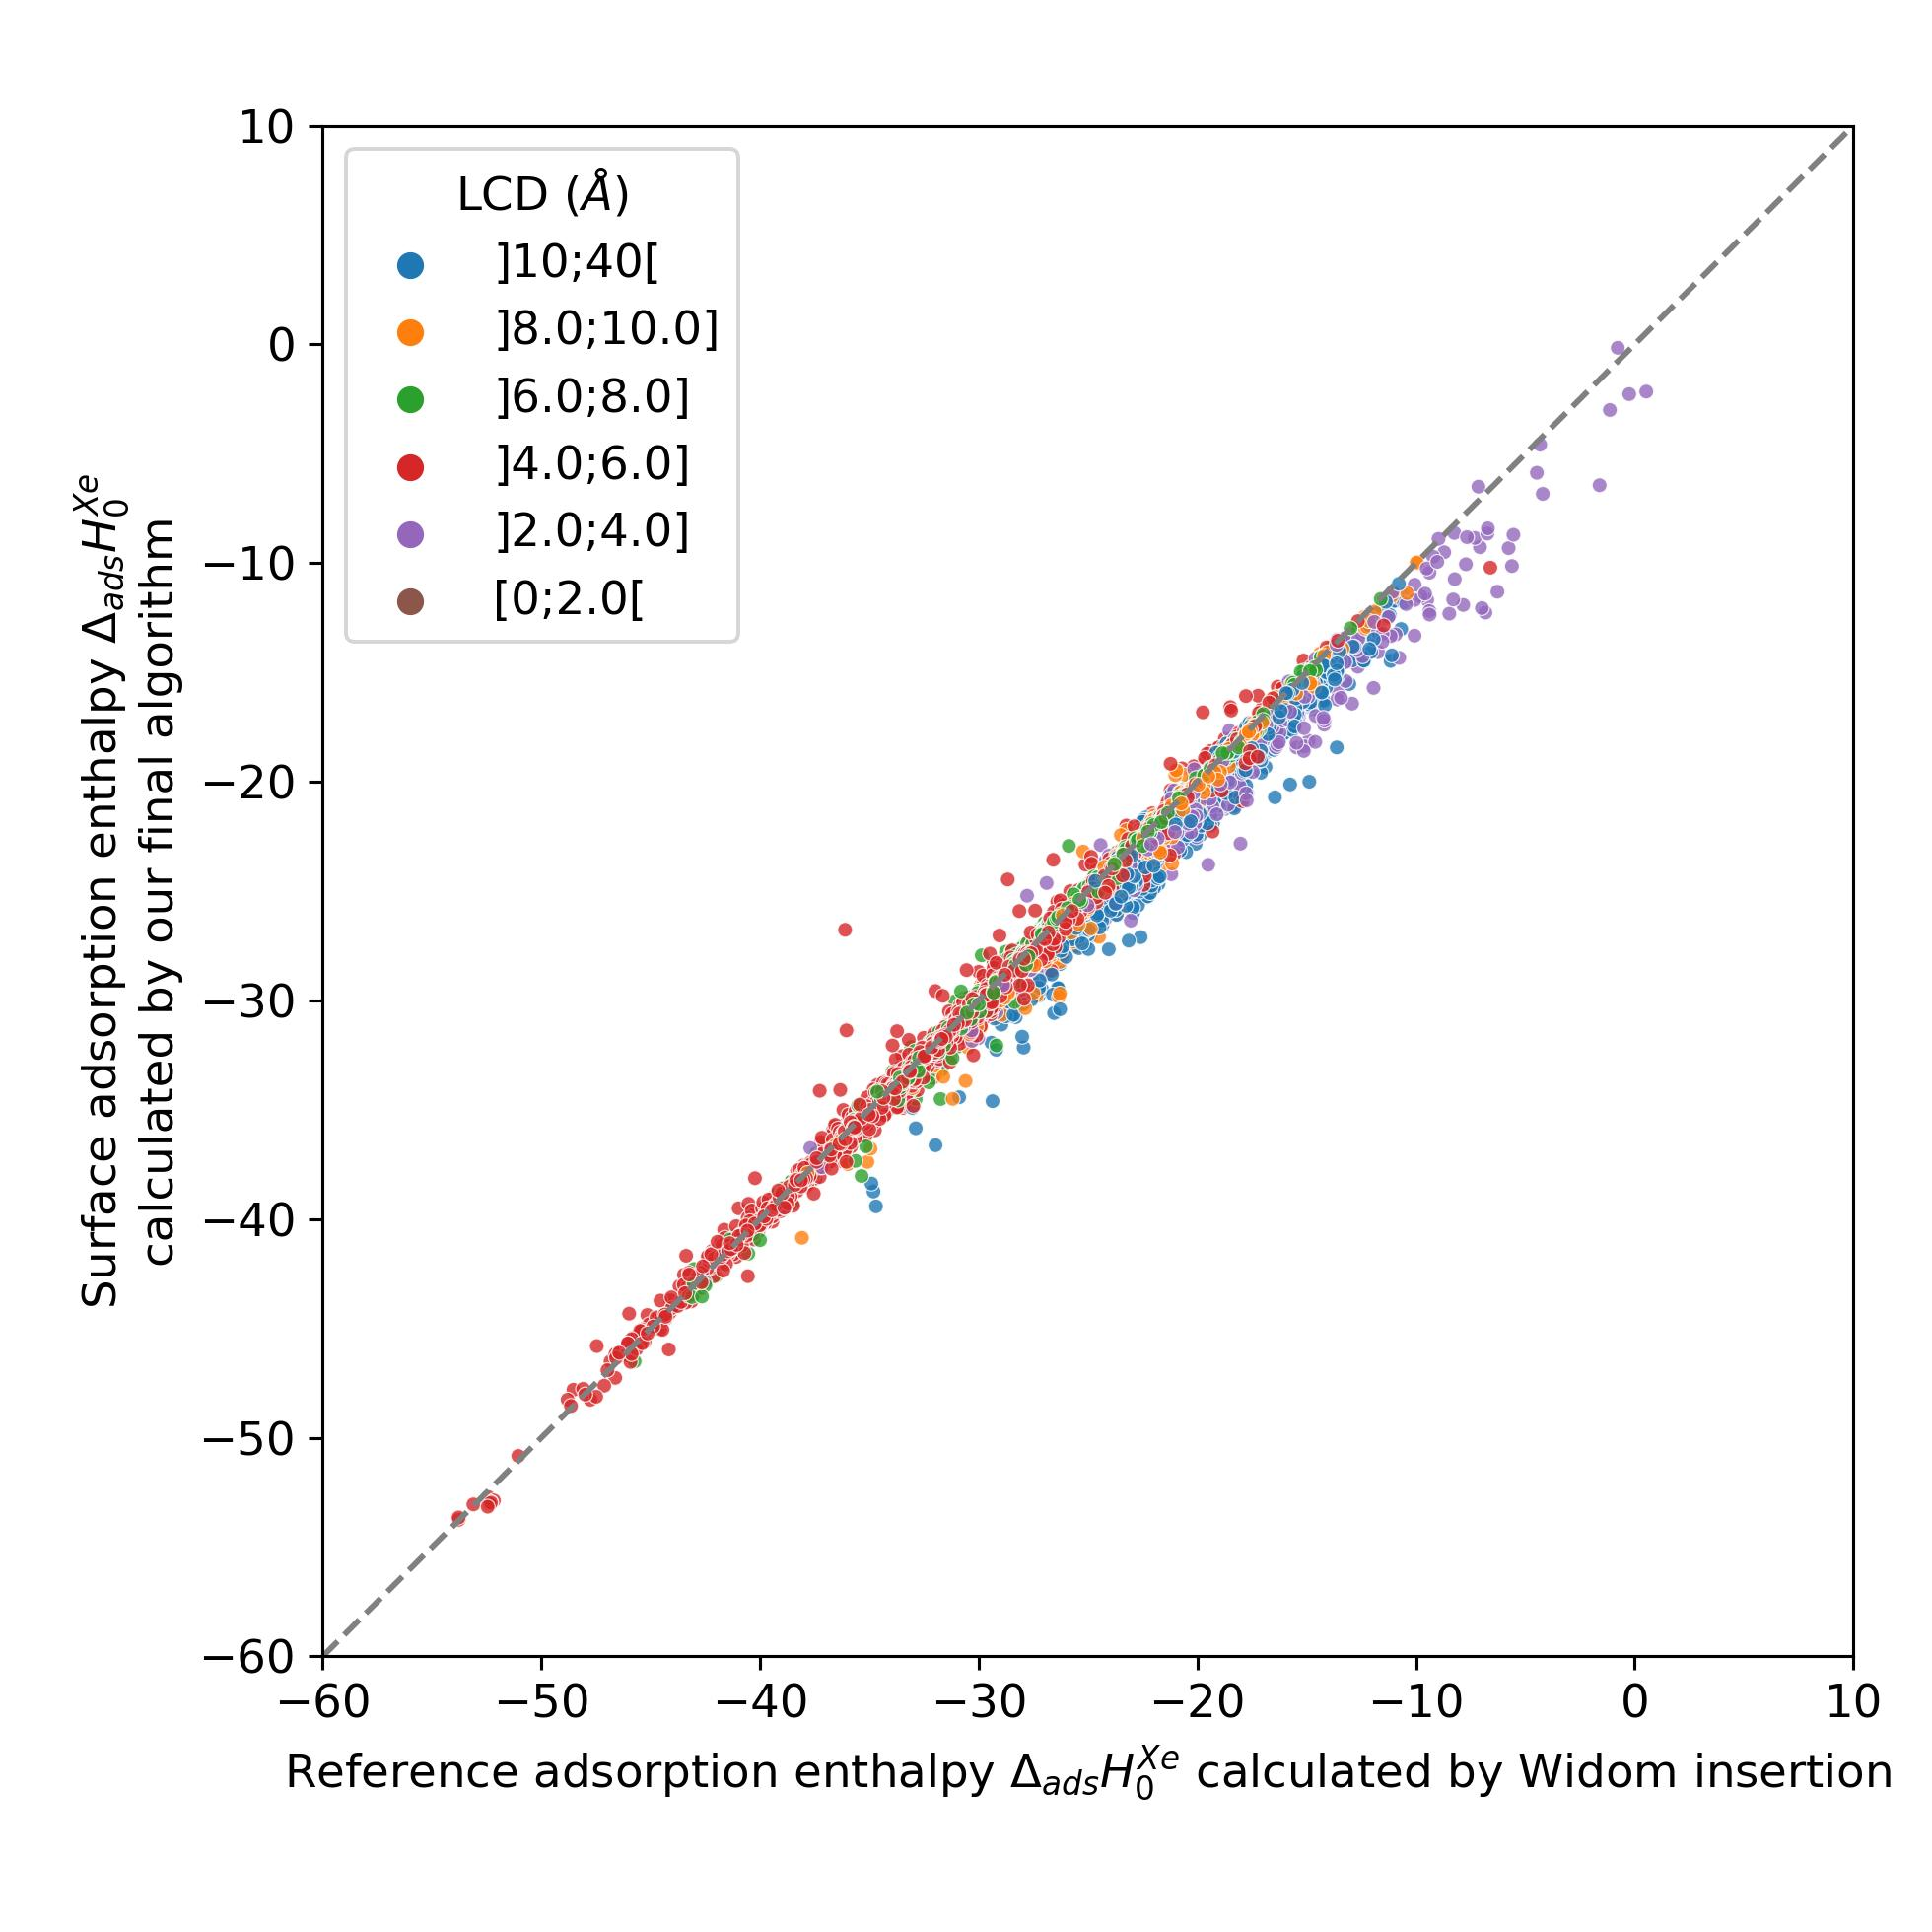
\includegraphics[width=0.5\linewidth]{figures/3-fastsim/H_Xe_widom_vs_H_Xe_surface_final_zoom_600K.jpeg}
  \caption{Scatterplot of the enthalpies calculated by our final algorithm ($\lambda=1.6$ and $\mu=0.85$) compared to the enthalpies calculated by a 12k step Widom insertion simulation of xenon in structures of CoRE MOF 2019 with LCD\e{CCDC} $\geq$ \SI{3.7}{\angstrom} at \SI{600}{\kelvin}. }
\end{figure}

The method is as expected less accurate, but it still gives a reasonable correlation on the performance, with an RMSE of \SI{0.70}{\kilo\joule\per\mole} and an MAE of \SI{0.41}{\kilo\joule\per\mole}. The errors have almost doubled when going from \SI{298}{\kelvin} to \SI{600}{\kelvin}. However, these limitations of the method are not crippling since adsorption processes are usually not performed at very high temperature. High temperatures are commonly used in temperature swing adsorption (TSA) to desorb the adsorbates rather than to adsorb them.

\subsubsection{Other databases}\label{sct:other_database}

\textbf{ToBaCCo}

We randomly selected 1,000 structures from the 13,511 porous frameworks of the ToBaCCo database to test the robustness of the RAESS method on a database other than CoreMOF. Since ToBaCCo contains structures with larger pores as suggested by a Moosavi et al., these materials are more unfavorable for adsorption of small molecules (such as Xe). The correlation is therefore found to be weaker than in the CoRE MOF 2019 database. This lower accuracy should be nuanced by the lack of suitability of these materials for Xe/Kr separation. Moreover, we can note that the points with weaker correlations correspond to the ones with an LCD\e{CCDC} greater than \SI{10}{\angstrom}, which is not ideal to separate Xe from Kr.

\begin{figure}[ht]
\centering
  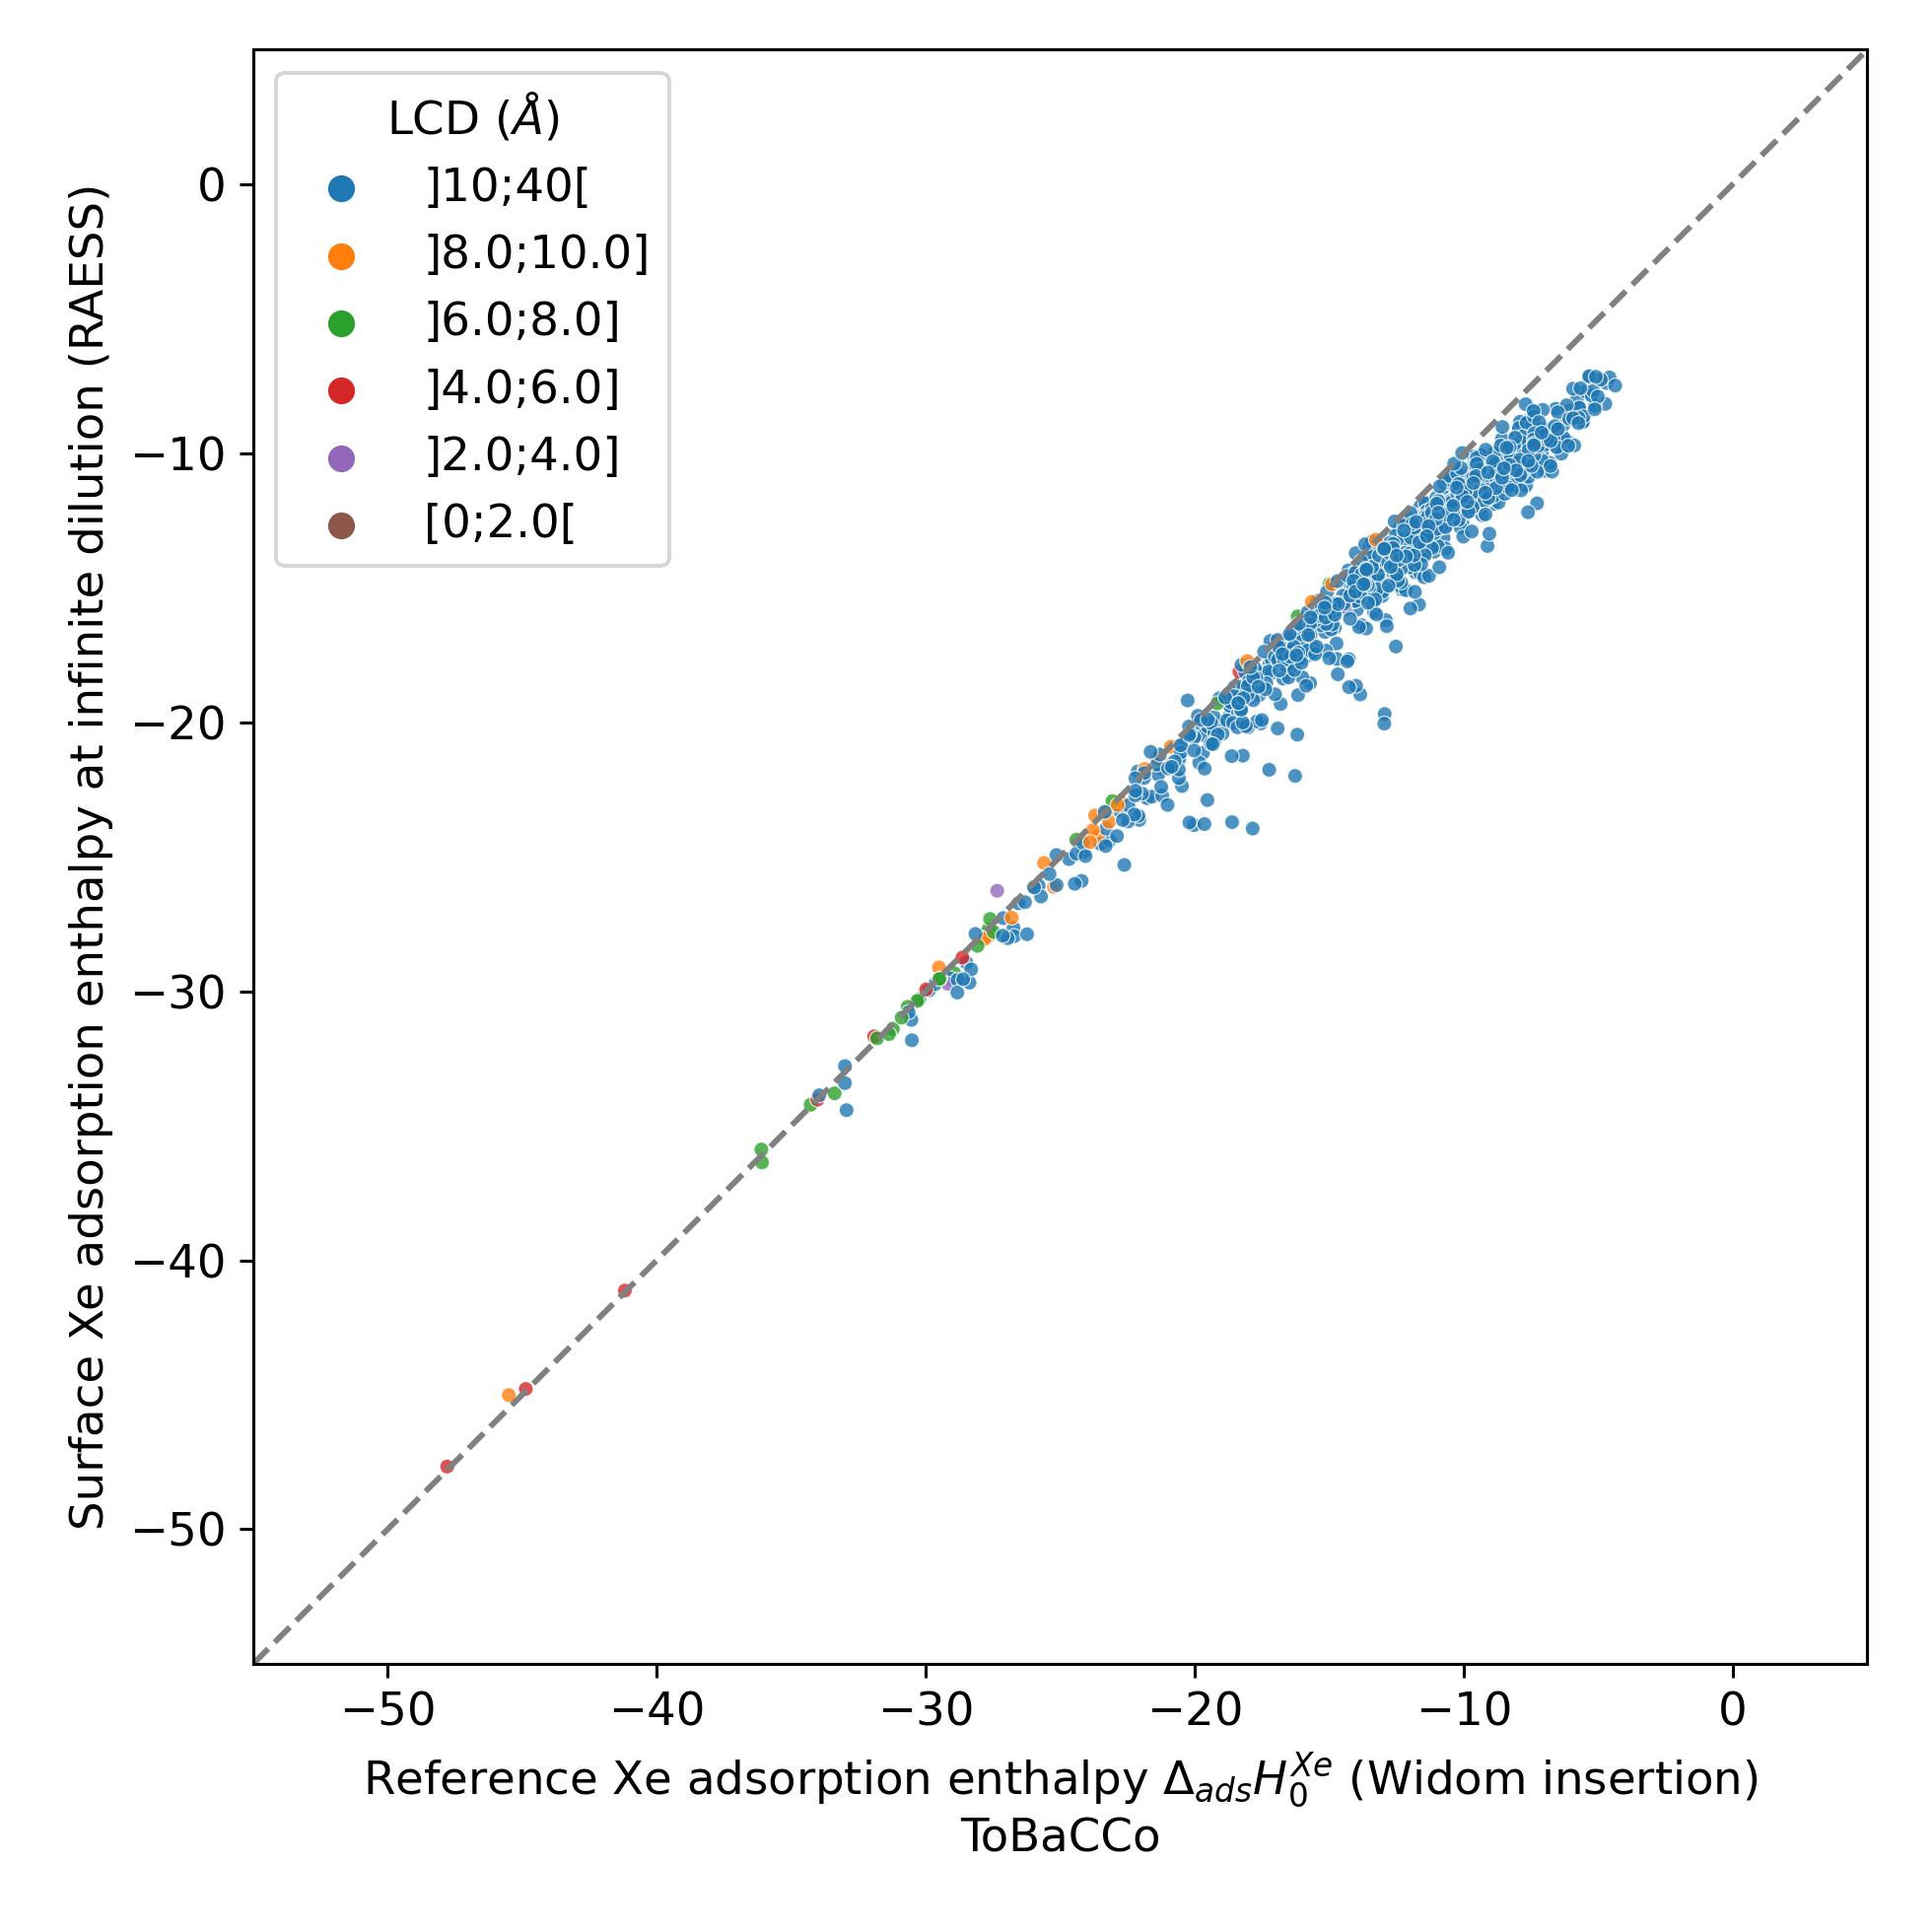
\includegraphics[width=0.5\linewidth]{figures/3-fastsim/H_Xe_0_widom_vs_Enthalpy_surface_kjmol_overview_tobacco.jpeg}
  \caption{Scatterplot comparison of the xenon adsorption enthalpy calculated by the RAESS algorithm and the Widom insertion (RASPA2) on the ToBaCCo database. RMSE = \SI{1.79}{\kilo\joule\per\mole} and MAE = \SI{1.48}{\kilo\joule\per\mole}. 915 structures have an LCD\e{CCDC} greater than \SI{10}{\angstrom}.}\label{fgr:tobacco}
\end{figure}

The algorithm performs very well on the most adsorptive materials with xenon adsorption enthalpy values lower than \SI{-30}{\kilo\joule\per\mole}, because for these materials the adsorption sites are located near the surface. For broader pore sizes, it is interesting to note some limitations of the methodology we should be aware of. For determining the most attractive materials, this shortcoming does not influence the final results. Moreover, this limitation is not that damaging since the correlation although weaker still remains.


\textbf{Amorphous materials}

To further extend the possible uses cases of the RAESS algorithm, we tested our algorithm on the amorphous database~\autocite{Thyagarajan_2020}. The algorithm found results for 176 structures out of 196. The RASPA2 software was not able to run on these amorphous structures with our computers, running out of memory due to the large system size: therefore, there is no comparison point with a Widom simulation. However, we used another simulation that is closer to the ground truth since it samples a homogeneously distributed grid using an optimized algorithm we will present in the next section. This grid sampling managed to compute the adsorption energies of 175 structures. 

The Table~\ref{tab:amorphous} gives the values of the adsorption enthalpies and the Henry constants of a few amorphous materials as well as the time they took to be computed. The sheer number of atoms in each structure makes the CPU time required much higher than for the crystalline structures of CoRE MOF 2019. The time required are, however, quite manageable in a hypothetical screening procedure. If we consider all the 175 structures that could be calculated by our methods, the average time required is about \SI{75}{\second} per structure. 

\begin{table}[hb]
  \begin{tabular}{|l|r|r|r|}
    \hline
    Structure Name & $\Delta\e{ads}H\e{0}\ex{Xe}$ (\SI{}{\kilo\joule\per\mole}) & $K\e{H}\ex{Xe}$ (\SI{}{\mole\per\kilo\gram\per\pascal}) & CPU time (s) \\
    \hline
    aCarbon-Marks-id035 &                 -63.55 &            6.98e-01 & 285.45 \\
    HCP-Colina-id016 &                 -30.61 &            8.85e-05 & 3.88 \\
    Kerogen-Coasne-id010 &                 -44.38 &            8.02e-03 & 61.2 \\
    PIM-Colina-id012 &                 -26.39 &            7.00e-05 & 8.86 \\
    \hline
    \end{tabular}
    \caption{Some amorphous materials' performance according to the RAESS algorithm. The results on the whole amorphous database is given in CSV format on the Github: \url{github.com/fxcoudert/citable-data/tree/master/154-Ren_ChemSci_2023}.}\label{tab:amorphous}
\end{table}

As we can see on the Figure~\ref{fgr:amorphous}, the accuracy of the surface sampling is rather high since by comparing it to an unbiased grid-based sampling, we obtain very similar results. The RMSE is about \SI{0.83}{\kJ\per\mol}, which is higher than the one for CoRE MOF structures. This method could very likely be used to evaluate amorphous materials as a fast screening tool especially since the computation time required by the optimized grid sampling is about \SI{623}{\second}. The dimension reduction inherent to the surface sampling makes it one order of magnitude faster than conventional techniques.

\begin{figure}[ht]
  \centering
  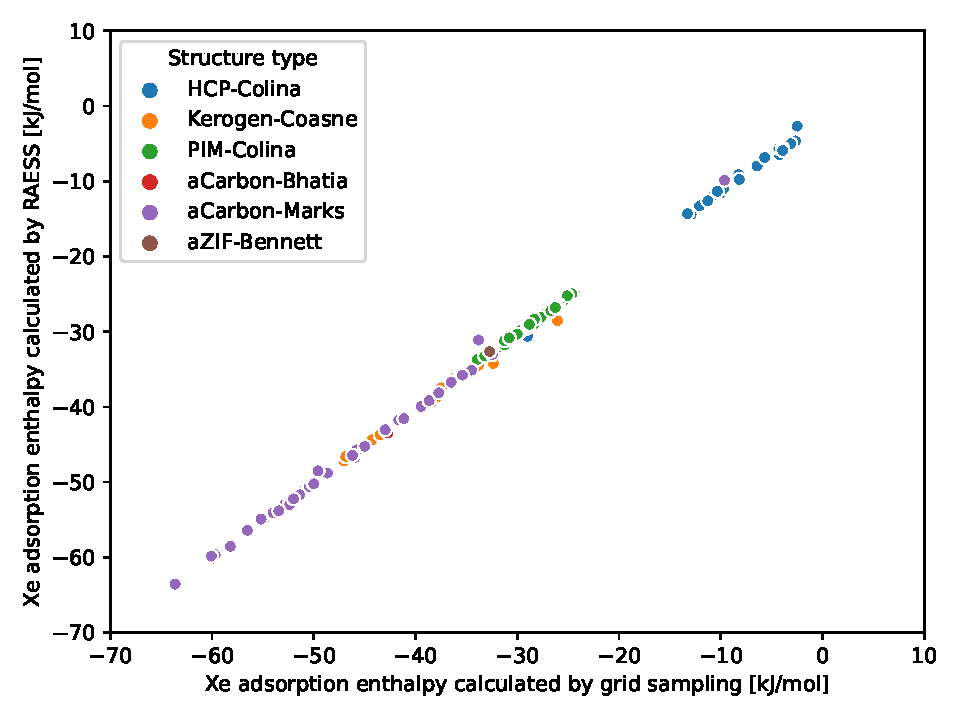
\includegraphics[width=0.5\linewidth]{figures/3-fastsim/amorphous_enthalpy.pdf}
  \caption{Scatterplot comparison of the xenon adsorption enthalpy calculated by the RAESS algorithm and the one calculated by a grid sampling (presented in the next section) on a database of porous rigid amorphous materials~\autocite{Thyagarajan_2020}. Raspa simulation could not be run on this database. Only the 175 structures computed by both methods are presented here. }\label{fgr:amorphous}
\end{figure}

\subsection{Perspectives of surface sampling}

We described a novel algorithm for the high-speed calculation of adsorption enthalpy in nanoporous materials, that takes a unique approach to reduce the sampling necessary. This new algorithm is based on the core principle of dimensional reduction, from a volume problem to a surface one. The algorithm is proven to be significantly faster than the reference Widom insertion (random sampling of porous space). Moreover, the error associated is found to be of the order of \SI{0.4}{\kilo\joule\per\mole}, tested throughout the entire CoRE MOF 2019 database, for xenon adsorption. Even when compared to existing very fast sampling techniques such as the Voronoi sampling, this surface sampling technique requires similar CPU time, combined with a better accuracy. 

Based on these results, this algorithm has important potential for applications in the current computational analysis workflows of material databases, such as high-throughput screening studies. For instance, this algorithm can be used to get a fast approximation of the low-loading adsorption enthalpy of a molecule inside nanoporous materials. This cheap evaluation of the enthalpy can be used to screen out the structures with little affinity with the targeted adsorbate molecule. It can also be used as a thermodynamic descriptor for selectivity prediction in a machine learning model, as done by Simon et al.\autocite{Simon_2015} The computational speedup brought by this novel methodology can also enable the screening of materials databases at larger scale in the future.

We note, moreover, that the speed of our method resides in the sampling technique itself, rather than in the actual energy calculation. While we have benchmarked it in this work for a simple Lennard-Jones interaction potential, this sampling technique could equally be used to speed up samplings of space based on more expensive modeling strategies, including polarizable force fields or density functional theory (DFT) calculations. In the literature, the need for cheap \emph{ab initio} grade thermodynamic properties is usually fulfilled by using an importance sampling method based on a classical force field.\autocite{Vandenbrande2018} In our method, the description of surface sampling is independent of any force field, and the sampling spheres can be defined according to kinetic radius, van der Waals radius or any other physically relevant distance. {Consequently, given a definition of atomic radii, it is possible to define a surface on which to carry out other types of simulations such as neural network potential, DFT or any other force fields. Although the accuracy or relevance of such a sampling remains an open question, the approach will undeniably speed up the simulations.} This could even be applied to calculate adsorption enthalpies while considering intrinsic structure flexibility,\autocite{Witman_2017} a task whose main drawback is the high computation time required. Since surface sampling is hundreds of times faster than standard methodologies, we could use hundreds of snapshots in a flexibility-aware calculation.

Finally, although the algorithm in its present form can already be applied in a wide range of applications, additional development work could allow us to generalize it to polyatomic adsorbates. For instance, we would need to {work on a definition of the molecular radius for non-spherical adsorbates as well as working} all the orientation conformation of the adsorbent. {We could imagine making the distance to the surface depend on the orientation of the adsorbate or sample a band volume on the surface. Although the best implementation of the surface sampling for polyatomic adsorbates remains an open question, in theory it should be possible to apply it to more complex adsorbates than the spherical noble gas. } This would add more complexity to the algorithm but would not change the fundamental speedup due to surface sampling, since these orientation moves are also performed in other standard methodologies. To improve even more the accuracy, we could test hybrid samplings with multiple sampling spheres, or a combination of Voronoi nodes and sampling spheres. Another idea could be to have fractions of spheres that are oriented toward the center of the pore given by the Voronoi node. In theory, having a wider variety of sampling points can only improve the sampling. There are therefore multiple possible sampling techniques that could be built around the method introduced herein. {The code is made freely available on the group's GitHub (\url{github.com/coudertlab/RAESS}), where further development will be released.}

\textbf{Data Availability:} \url{https://github.com/fxcoudert/citable-data/tree/master/154-Ren_ChemSci_2023}

\section{Grid Adsorption Energies Descriptors (GrAED)}\label{sct:grid}

\subsection{Implementation of an efficient grid algorithm}

To build more relevant energy descriptors, we will now go back to the definitions of the adsorption enthalpy and the Henry constant (equation~\ref{eq:ads_enthalpy} and~\ref{eq:henry}) that call for a homogeneous sampling of the adsorption space. The easiest way of sampling consists in laying a grid in the 3D space. This method is, however, known to be the most time-consuming on in theory. Inspired by our work on surface sampling, we designed an approach based on a symmetry-respecting grid,generated using the algorithms of the Gemmi Project,\autocite{Wojdyr_2022} where the points overlapping with framework are discarded. In our grid adsorption energy descriptor (GrAED) calculation algorithm, these new features coupled with a grid sampling makes the calculation of adsorption energies much less time-consuming while being very accurate.

\begin{figure}[ht]
  \centering
    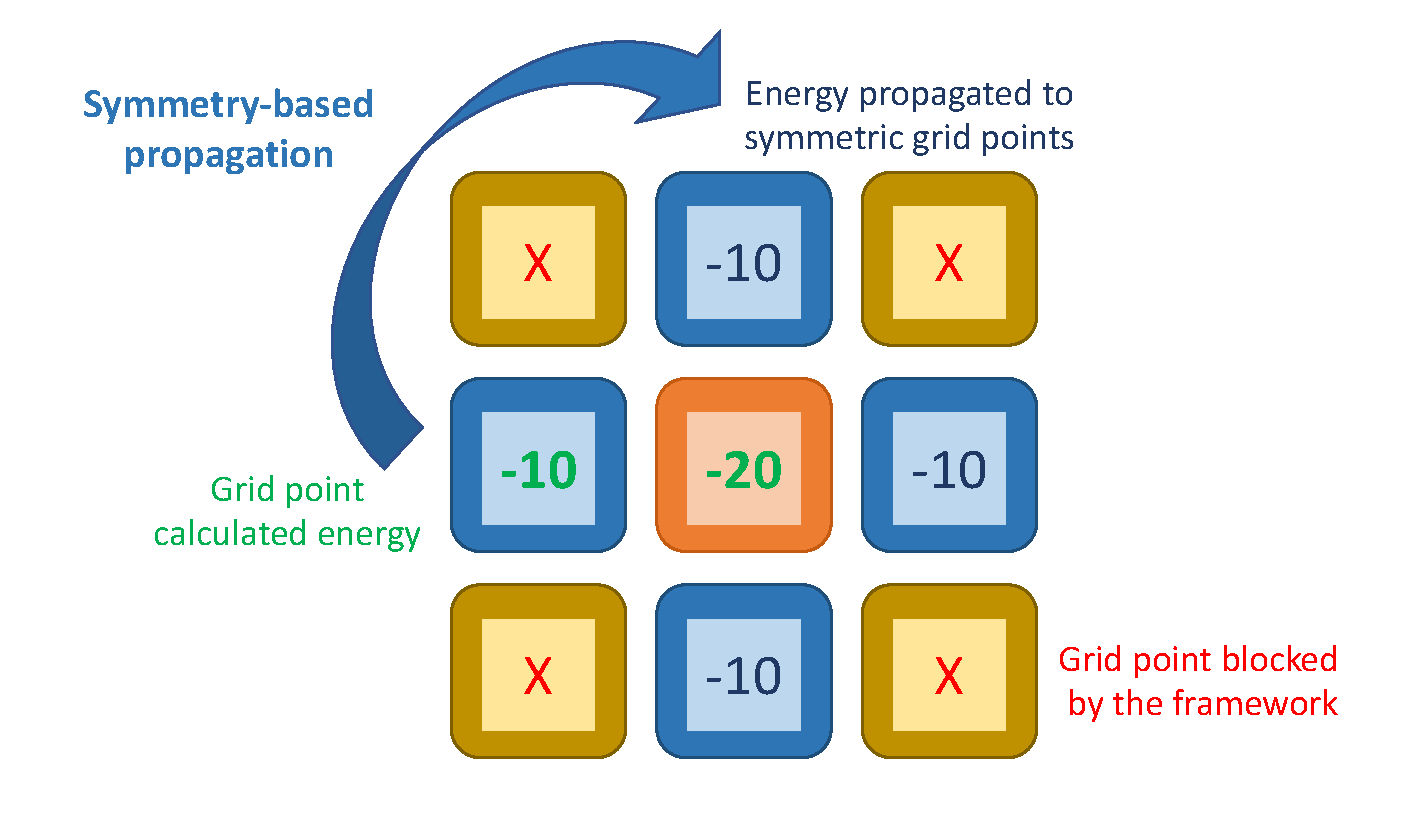
\includegraphics[width=0.5\textwidth]{figures/3-fastsim/grid_sampling.pdf}
    \caption{Principle of the energy sampling on a symmetry-based grid. On the 9 grid points, 4 points are blocked because they are too close to the framework atoms, 2 points are really calculated using the LJ potential and 3 points are propagated using the inner symmetry of the framework.}\label{fgr:principle_grid}
\end{figure}

The corresponding algorithm has a core structure of a grid algorithm, where we need to evaluate the interaction energy at each point of the preset grid over the structure's unit cell. A naive approach would call for an expensive energy calculation at each grid point. To improve this approach, our algorithm is based on two main simplifications --- a quick evaluation of the framework occupied grid points and the exploitation of symmetry. The grid points that overlap with the framework's atoms have highly positive energy mainly due to the interaction with the overlapping atom. High values of energy does not contribute much to any thermodynamic quantities displayed in the section~\ref{sct:thermo}. For this reason by using a rejection parameter similar to the one developed for surface sampling introduced in the section~\ref{sct:rejection_condition}, we can precalculate the interaction energy of the grid points within the sphere of radius $\mu\times\sigma_{g-h}$. If the value of this interaction energy is higher than a preset energy threshold $E\e{th}$, then the associated grid point takes these values as the interaction energy and no further calculation will be performed for it. The symmetry of the grid is based on the symmetry of the structure determined using the Grid definition of the Gemmi Project. By using the symmetry operations on a grid point value, we can propagate it to the other symmetry-equivalent grid points as illustrated in the Figure~\ref{fgr:principle_grid}, which reduces the amount of time we need to calculate the interaction energy of a guest molecule at a given grid node with all the surrounding framework atoms within a given cutoff. Now that we presented the main building blocks of our optimized grid calculation, we will show how it integrates in the implementation of the algorithm.

\begin{enumerate}
  \item We loop over the framework atoms and the grid points around a sphere of radius $\mu\times\sigma_{g-h}$, where $\sigma_{g-h}$ is the distance at which the LJ potential energy between the guest atom $g$ and the host atom is zero. The LJ potential energy between the guest molecule and the closest host atom is calculated and only the grid points with an energy lower than a predefined threshold $E\e{th}$ are considered ``unvisited'' and will be recalculated in the following loop, the others are considered blocked by the framework and will be considered already ``visited''. This first loop over the framework atoms aims at filtering out the grid points that are blocked by the framework, and we will refer to this preliminary filtering step as ``blocking'' in the Table~\ref{tab:grid}.
  \item A second loop over the ``unvisited'' grid points is performed --- at each increment, if the point is ``unvisited'' we calculate the interaction energy between the guest and all the host atoms within the cutoff, then the symmetric images of this point are filled with the same energy value and are considered ``visited'' by the algorithm. This symmetry-aware grid exploration allows the algorithm to divide the time required by the average number symmetry images --- this module will be referred to as ``symmetry'' in the Table~\ref{tab:grid}.
\end{enumerate}

By combining both the ``blocking'' of the high energy grid points and the ``symmetry'' based calculation of the interaction energies, we built a ``fast'' version of the grid calculation algorithm that can compete with our previously developed rapid surface sampling method (RAESS). To control the trade-off between accuracy and computation time, we can vary the spacing between the grid points, whose computation time is theoretically inversely proportional to the cube of the spacing. And, for some values of this spacing, this algorithm can even be faster than the surface sampling on the CoRE MOF database where the symmetry plays an important role (see Table~\ref{tab:grid}). The full implementation of the GrAED algorithm can be found at the following Github url: \url{github.com/coudertlab/GrAED.git}.

\subsection{Performance on the adsorption equilibrium}

If we now look at the performance of this new grid sampling algorithm compared to other sampling algorithms introduced in the previous sections. We can see that it is very advantageous to use this new sampling on the CoRE MOF 2019 database because of its accuracy and its speed.
The good time performance of the grid sampling on the structures of CoRE MOF 2019 database can be explained by their rather small porosity of the materials and their high order of symmetry. For instance, the average void fraction for a \SI{1.2}{\angstrom} probe radius is equal to $0.16$ and the average number of symmetric images is equal to $5.8$ (most MOFs present symmetry operations). On average, the ``blocking'' procedure means that only {$\sim$16\%} of the grid points really need to be calculated. And the ``symmetry'' procedure implies that only {$\sim$17\%} of points need to be considered, and the combination of both theoretical reduces the number of useful points to only {2.7\%} of the grid. This leads to a significant reduction in the CPU time of the calculation while keeping the accuracy level (low error on the Xe adsorption enthalpy \SI{0.014}{\kilo\joule\per\mole}) compared to the naive grid approach, as shown in Table~\ref{tab:grid}. In the grid simulation, with the blocking procedure, the time required is reduced by {$\sim$70.6\%} compared to the naive approach, and a similar reduction of {$\sim$76.6\%} is observed for the symmetry-aware grid sampling. By combining both simplifications, the time required of the fast grid sampling is reduced by almost {$\sim$91.6\%} for a grid spacing of \SI{0.12}{\angstrom}, which echoes with the fewer points needed to be sampled we mentioned above.

\setlength{\extrarowheight}{0.1cm}
\begin{table}[ht]
  \centering
  \begin{tabular}{|l|r|r|}
    \hline
    Energy sampling  & RMSE on xenon  &  Average CPU  \\
    method  & adsorption enthalpy (\si{\kilo\joule\per\mole}) &  time (s) \\[0.5mm]
    \hline
    Grid -- naive -- \SI{0.12}{\angstrom} & 0.014  &  35.4 \\[0.5mm] 
    Grid -- blocking -- \SI{0.12}{\angstrom} & 0.014  &  10.4 \\ 
    Grid -- symmetry -- \SI{0.12}{\angstrom} & 0.014  &  8.3 \\ 
    Grid -- fast -- \SI{0.12}{\angstrom} & 0.014  &  2.96 \\
    Grid -- fast -- \SI{0.2}{\angstrom} & 0.048  &  0.41 \\
    Grid -- fast -- \SI{0.3}{\angstrom} & 0.21  &  0.13 \\
    Voronoi sampling &   2.1  & 0.40 \\
    RAESS\autocite{Ren_2023} & 0.33   &  0.34 \\
    Widom\autocite{Widom1963} (12k cycles) & 0.038  &  150 \\
    \hline
  \end{tabular}
  \caption{Performance comparison of the new grid method to other standard techniques used to calculate the xenon adsorption enthalpies. The RMSE is calculated by comparing to the values given by a 100k-step Widom insertion considered as the ground truth. The associated calculations are performed on the structures with an LCD\e{CCDC} over \SI{3.7}{\angstrom} of CoRE MOF 2019 database with a single Intel Xeon Platinum 8168 core at 2.7~GHz. The GrAED algorithm (with$\mu=0.8$ $E\e{th}=$\SI{100}{\kilo\joule\per\mole}) is evaluated at different grid spacings ($0.12$, $0.20$, $0.30$).}\label{tab:grid}
\end{table}

% \todo{Beatify figure with arrow}

\begin{figure}[ht]
  \centering
    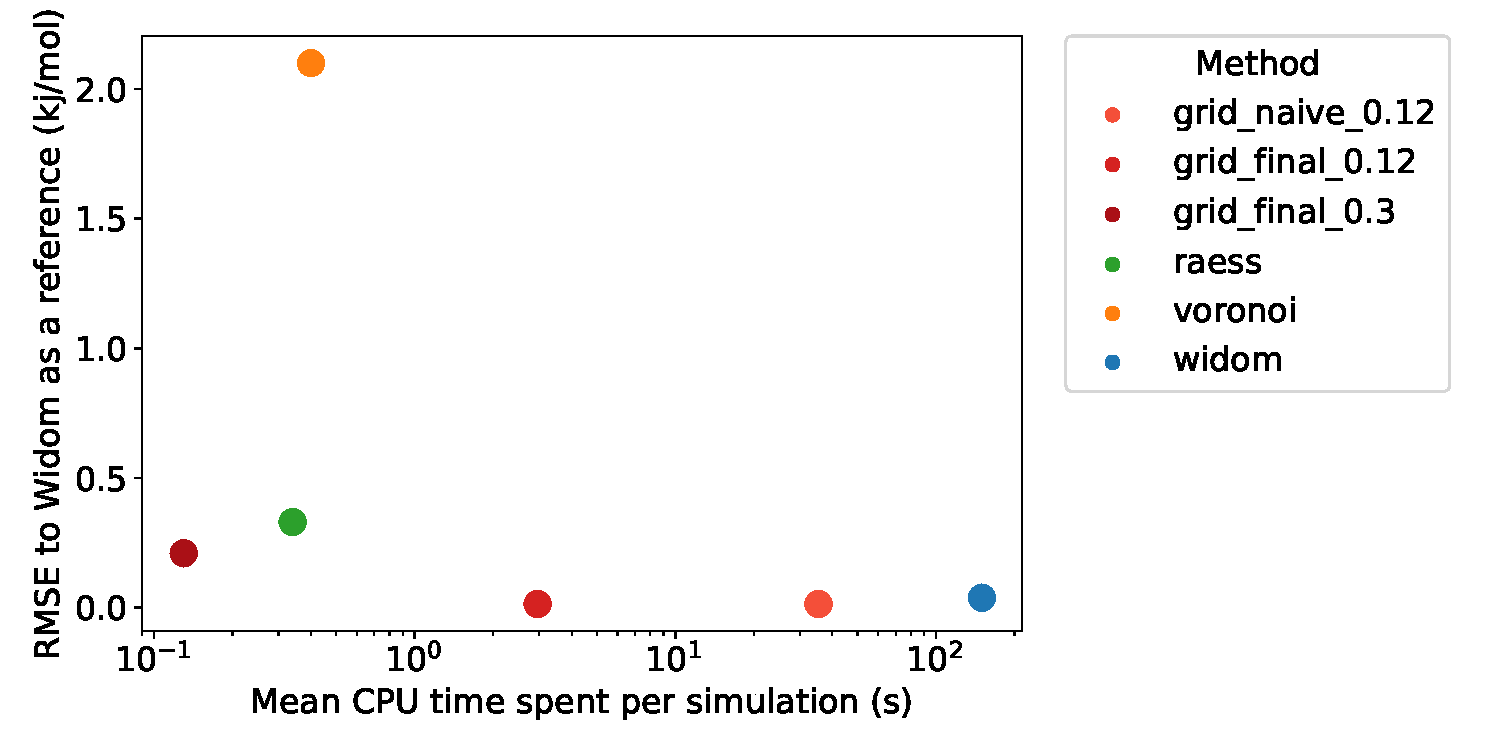
\includegraphics[width=0.7\textwidth]{figures/3-fastsim/Sum-up_grid.pdf}
    \caption{Comparison of the RMSE on Xe adsorption enthalpy and the average CPU time required to run a simulation on a structure of CoRE MOF 2019 (LCD\e{CCDC} $\geq$ \SI{3.7}{\angstrom}). The metrics are taken from the Table~\ref{tab:grid}. }\label{fgr:grid_perfomance}
\end{figure}

As we can see of the Figure~\ref{fgr:grid_widom}, the approach does not damage the accuracy of the adsorption enthalpy and of the Henry constant. There is an almost perfect accordance between the Widom insertion method and the grid-based approach for a very finely meshed grid (\SI{0.12}{\angstrom} spacing). This was expected since both methods are unbiased sampling of the adsorption energies. Almost no error can be detected if looking at the figure for both adsorption enthalpy and Henry constant. The RMSE on the adsorption enthalpy is only about \SI{0.01}{\kilo\joule\per\mole}, while the RMSE on the log10 of the Henry constants (in \si{\milli\mole\per\gram\per\pascal}) is also very low at $0.01$. This method goes back to the initial definition of these quantities at infinite dilution, the perfect correspondence is therefore not very surprising. 

\begin{figure}[ht]
  \centering
    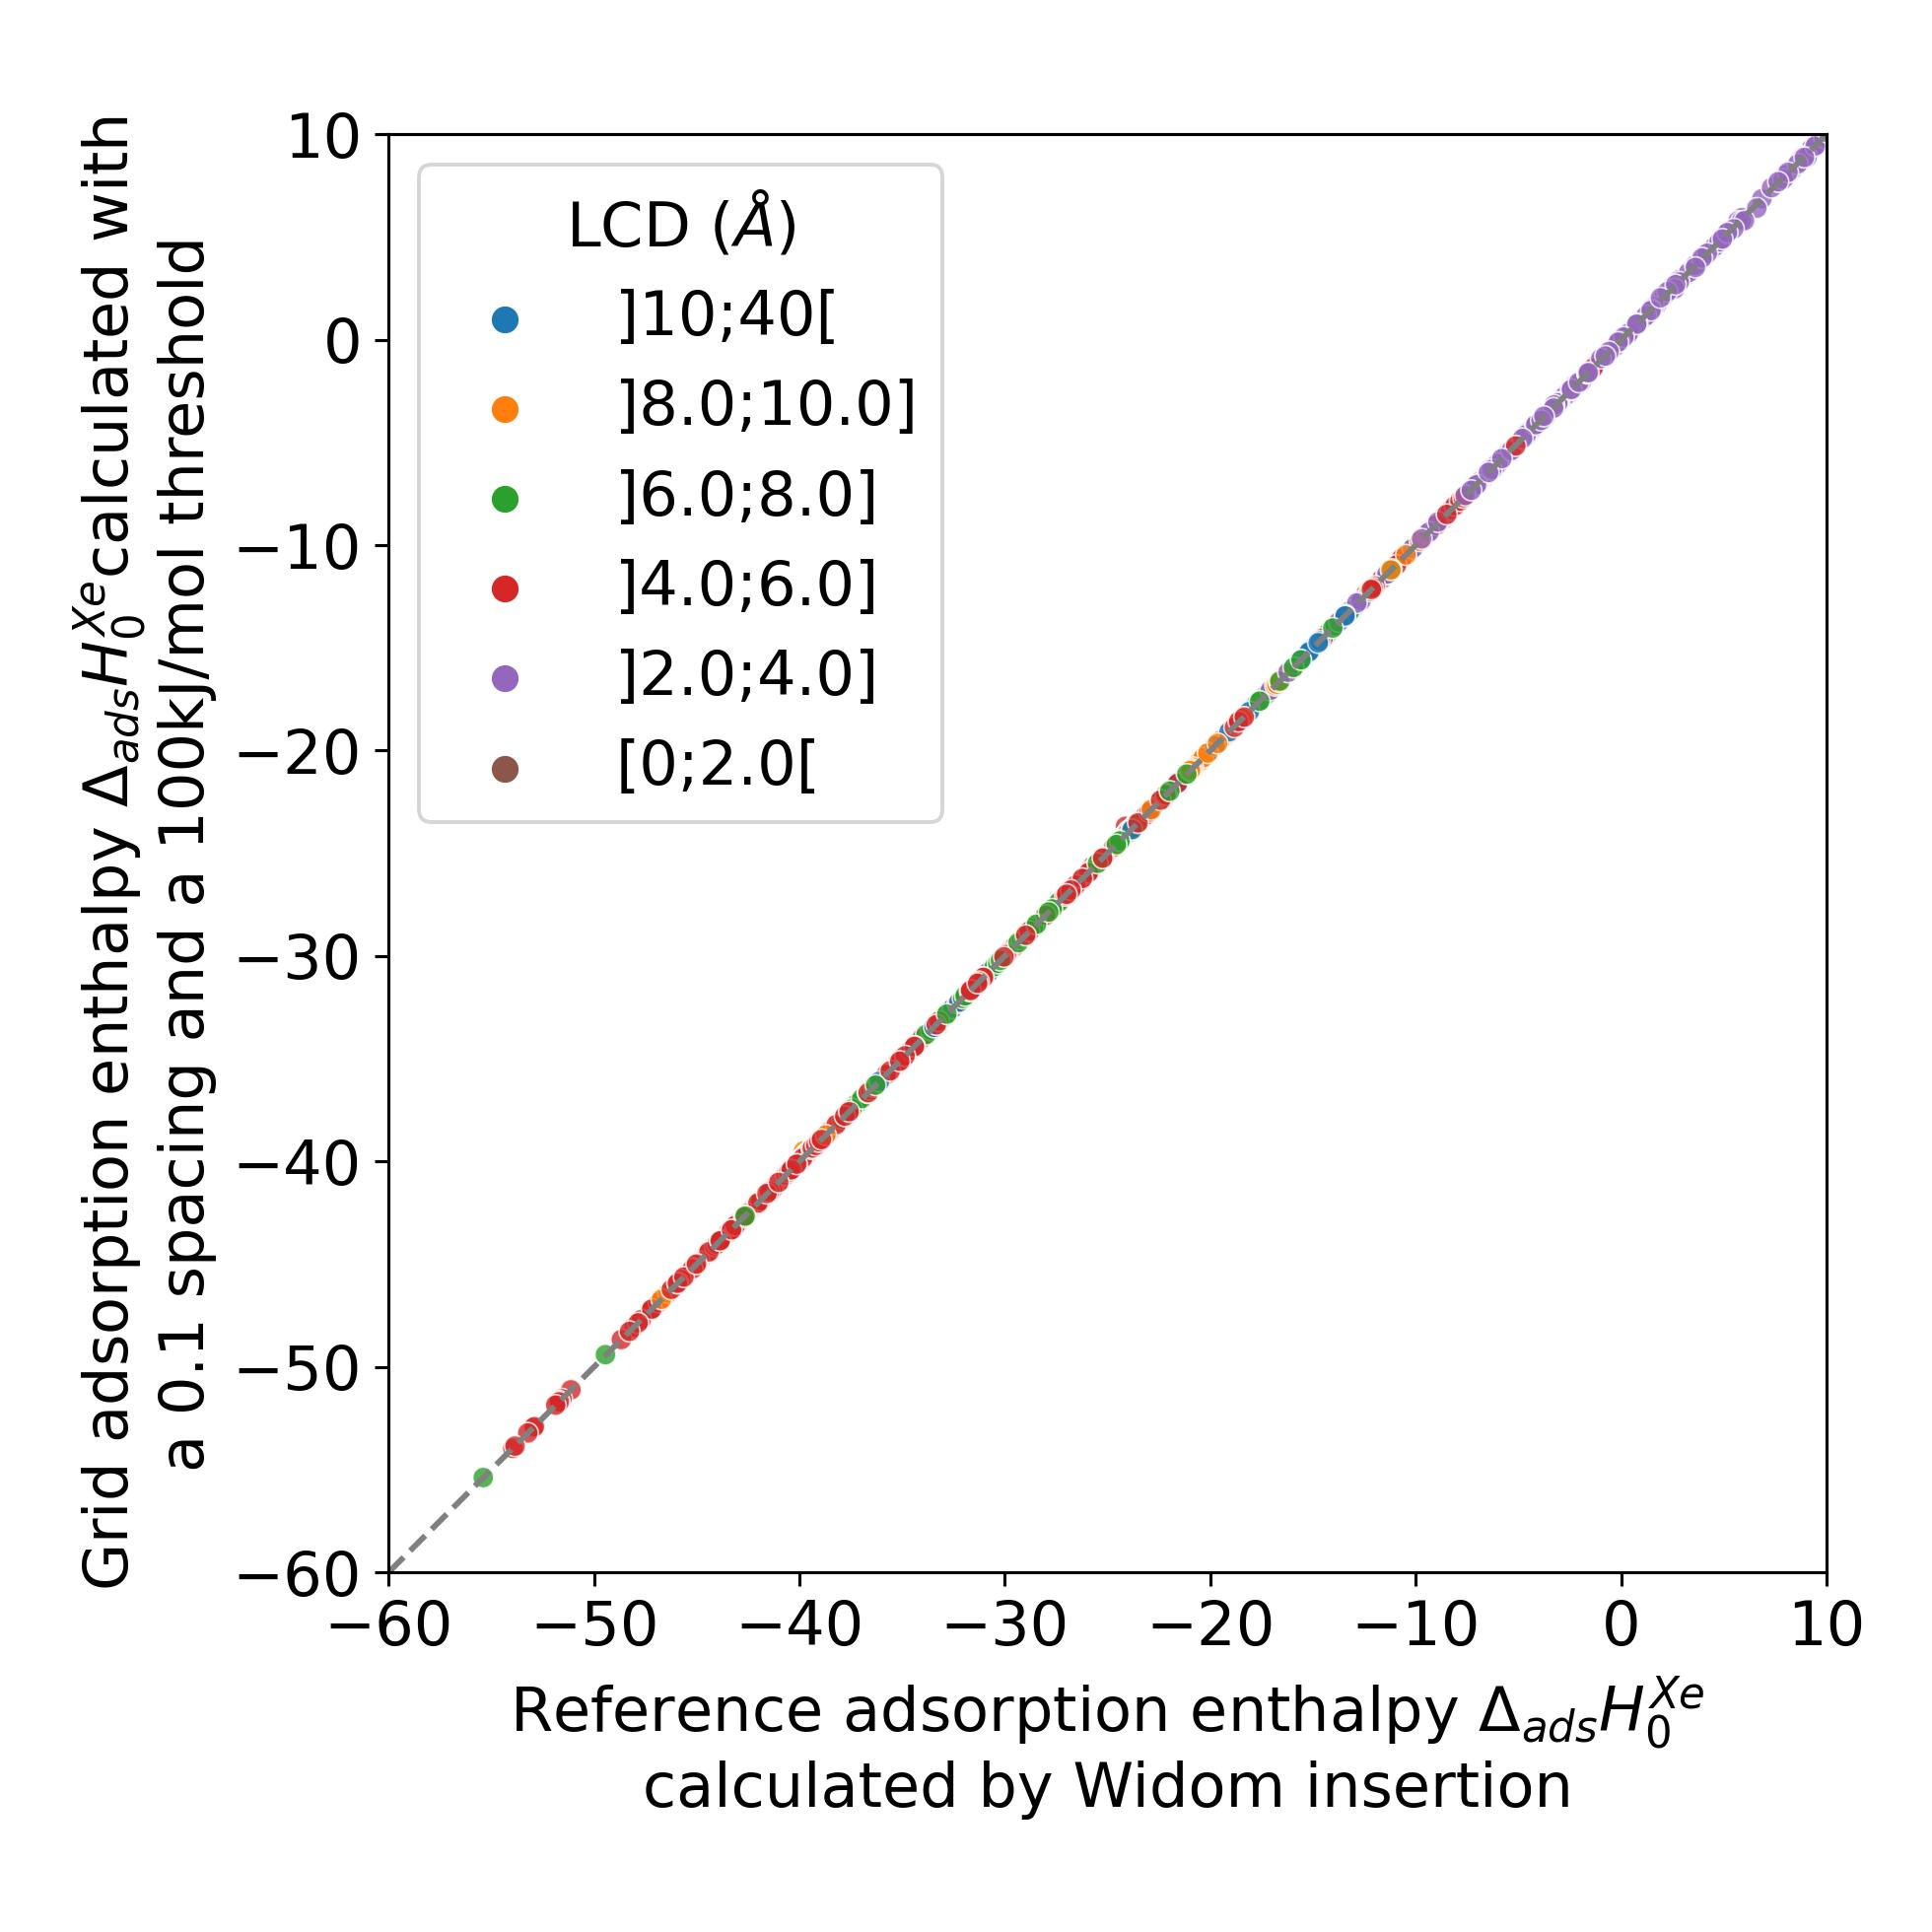
\includegraphics[width=0.45\textwidth]{figures/3-fastsim/H_Xe_widom_vs_H_Xe_grid_overview.jpg}
    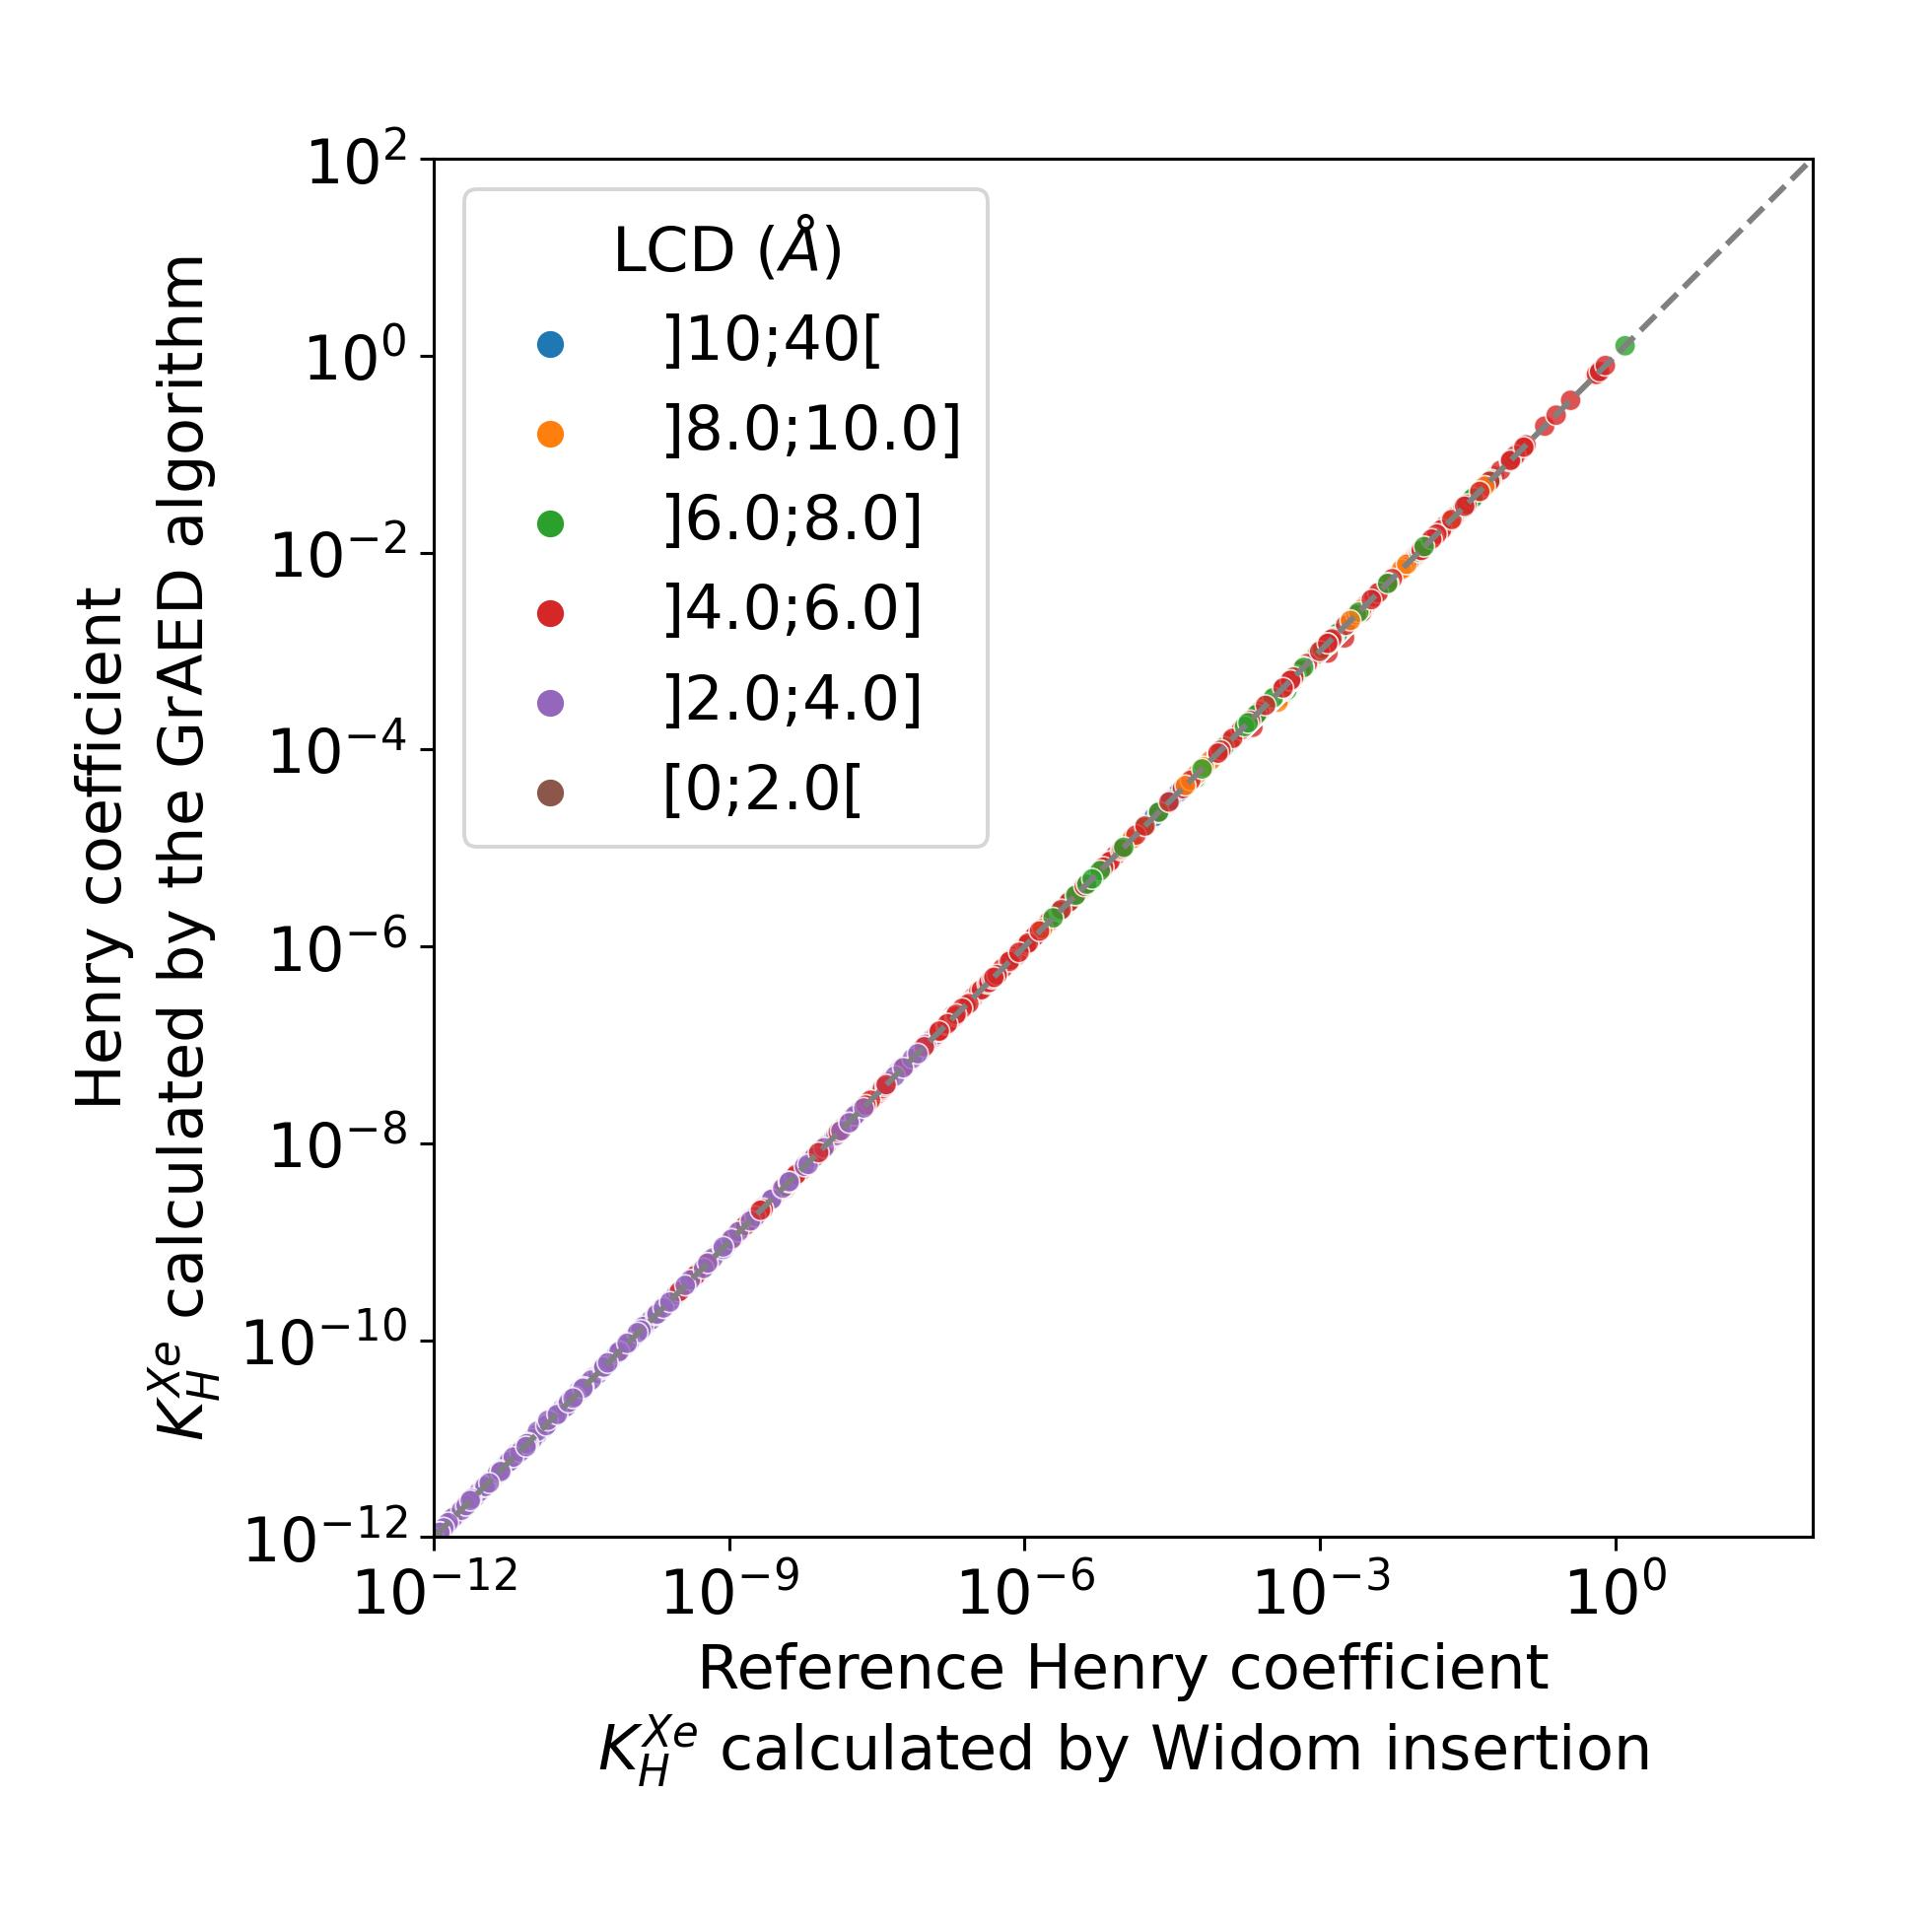
\includegraphics[width=0.45\textwidth]{figures/3-fastsim/K_Xe_widom_vs_K_Xe_grid_overview.jpg}
    \caption{Comparison of the xenon adsorption enthalpies (left) and the Henry constants (right) calculated by the optimized grid energy sampling (for a \SI{0.12}{\angstrom} spacing, a rejection parameter $\mu=0.8$ and an energy threshold $E\e{th}$ of \SI{100}{\kilo\joule\per\mole}) and by the Widom insertion of RASPA with 100,000 cycles on the CoRE MOF 2019 structures (LCD\e{CCDC} $\geq$ \SI{3.7}{\angstrom}). }\label{fgr:grid_widom}
\end{figure}

The little computation time required to achieve such an accuracy is, however, much more interesting. If we look at the Table~\ref{tab:grid}, the very accurate grid sampling reaches a similar accuracy than a 12k-cycle Widom insertion calculated using the Raspa software, while being 50 times faster. On the CoRE MOF 2019 database, by using a looser grid spacing of \SI{0.3}{\angstrom}, the GrAED algorithm can even be more interesting than the RAESS algorithm since it halves the computation time while being slightly more accurate. This very comparable performance compared to a dimensionally reduced sampling technique can be explained by two factors of the CoRE MOF database: first, the structures have smaller pores which means a greater surface to volume ratio, which increase the RAESS computation time; second, the highly symmetric structures of CoRE MOF reduces considerably the computation time required for GrAED, and the same cannot be said for other databases such as ToBaCCo or the amorphous database we studied section~\ref{sct:other_database}. 

For instance, the computation time required is found to be 750 times higher for a grid sampling than a surface sampling on the amorphous database (see section~\ref{sct:other_database}), and the RMSE is only of \SI{0.83}{\kJ\per\mol}. For amorphous databases, the surface sampling would be much better than an exhaustive grid sampling because both symmetry and overlap consideration reduce much less the number of sampled points, and we see the effect of surface sampling dimension reduction much more than on the CoRE MOF database. If we now take a look at the ToBaCCo database,\autocite{Colon_2017} the symmetry does not play any role anymore, and the pores are much larger, which means less points blocked by the framework. This impacts directly the performances of the grid sampling compared to the RAESS algorithm. The average time required on the thousand structures of ToBaCCo, considered in section~\ref{sct:other_database}, is now \SI{735}{\s} instead of less than \SI{2}{\s} for a surface sampling. By increasing the grid spacing to $0.3$, we can expect to reduce time required to \SI{47}{\s} with a simple application of the rule of three. The accuracy however is much better than for a surface sampling (see Figure~\ref{fgr:grid_tobacco}), reaching an extremely low RMSE of \SI{0.02}{\kJ\per\mol}. Depending on the number of structures and their nature (symmetry, porosity), we need to choose between the more efficient but less accurate RAESS and the GrAED software.

\begin{figure}[ht]
  \centering
    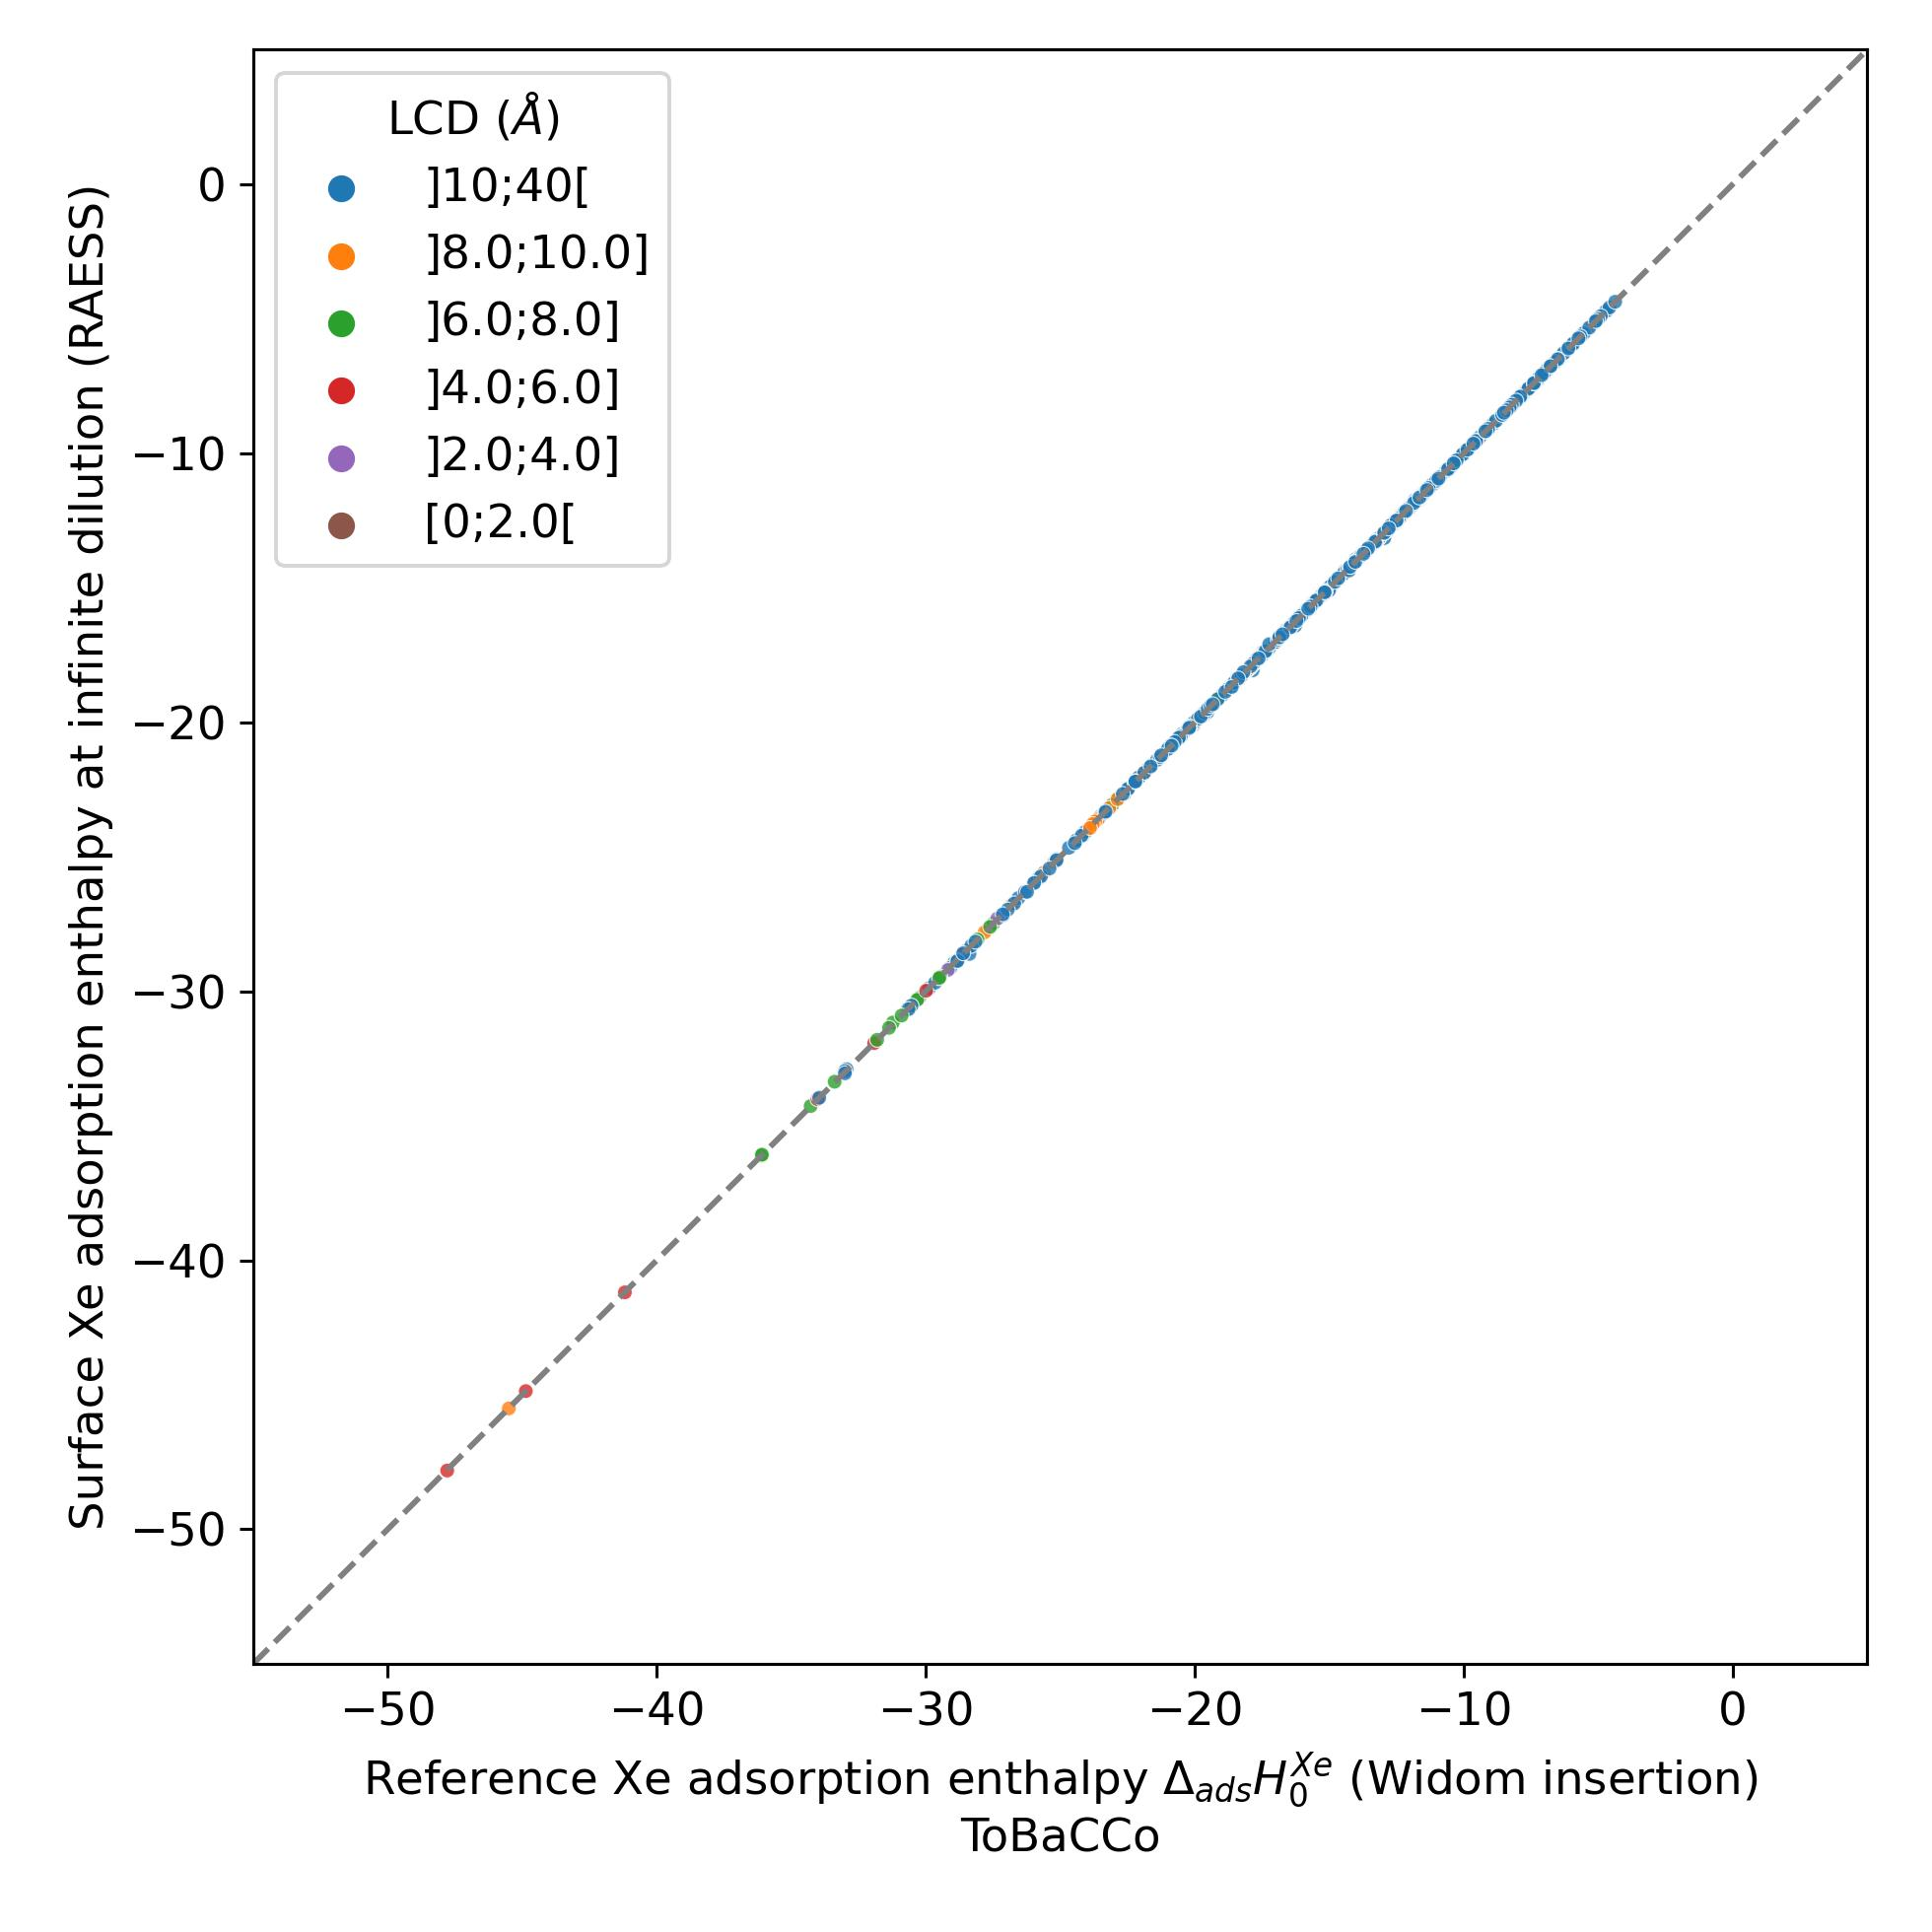
\includegraphics[width=0.45\textwidth]{figures/3-fastsim/H_Xe_0_widom_vs_Enthalpy_grid_kjmol_overview_tobacco.jpeg}
    \caption{Comparison of the xenon adsorption enthalpies (left) and the Henry constants (right) calculated by the optimized grid energy sampling (for a \SI{0.12}{\angstrom} spacing, a rejection parameter $\mu=0.8$ and an energy threshold $E\e{th}$ of \SI{100}{\kilo\joule\per\mole}) and by the Widom insertion of RASPA with 100,000 cycles on 1000 randomly selected structure of the ToBaCCo.\autocite{Colon_2017} }\label{fgr:grid_tobacco}
\end{figure}

From the energy values of this grid, we can now calculate many useful descriptors of the adsorption process. We have seen the performance on the Xe adsorption enthalpy and the Xe Henry constant. But as mentioned in the section~\ref{sct:thermo}, we can also derive the Xe adsorption Gibbs free energy and the Xe adsorption entropy. If we now consider the krypton in addition to the xenon, we can naturally evaluate the Kr adsorption thermodynamic quantities but also the exchange thermodynamic quantities and especially the Xe/Kr selectivity (the key metric in evaluating the separation process we are interested in).


\subsection{Performance on the exchange equilibrium}

To characterize the competitive adsorption of the binary mixture of xenon and krypton we commonly use the Xe/Kr selectivity. Compared to a single component metric like the Henry constant, the relative uncertainty will mechanically increase since the selectivity is a quotient of the Henry constants of the competitive adsorbates. In this section, we want to measure this error and see if it is relevant to characterize the separation with this optimized grid sampling method.

\begin{figure}[ht]
  \centering
    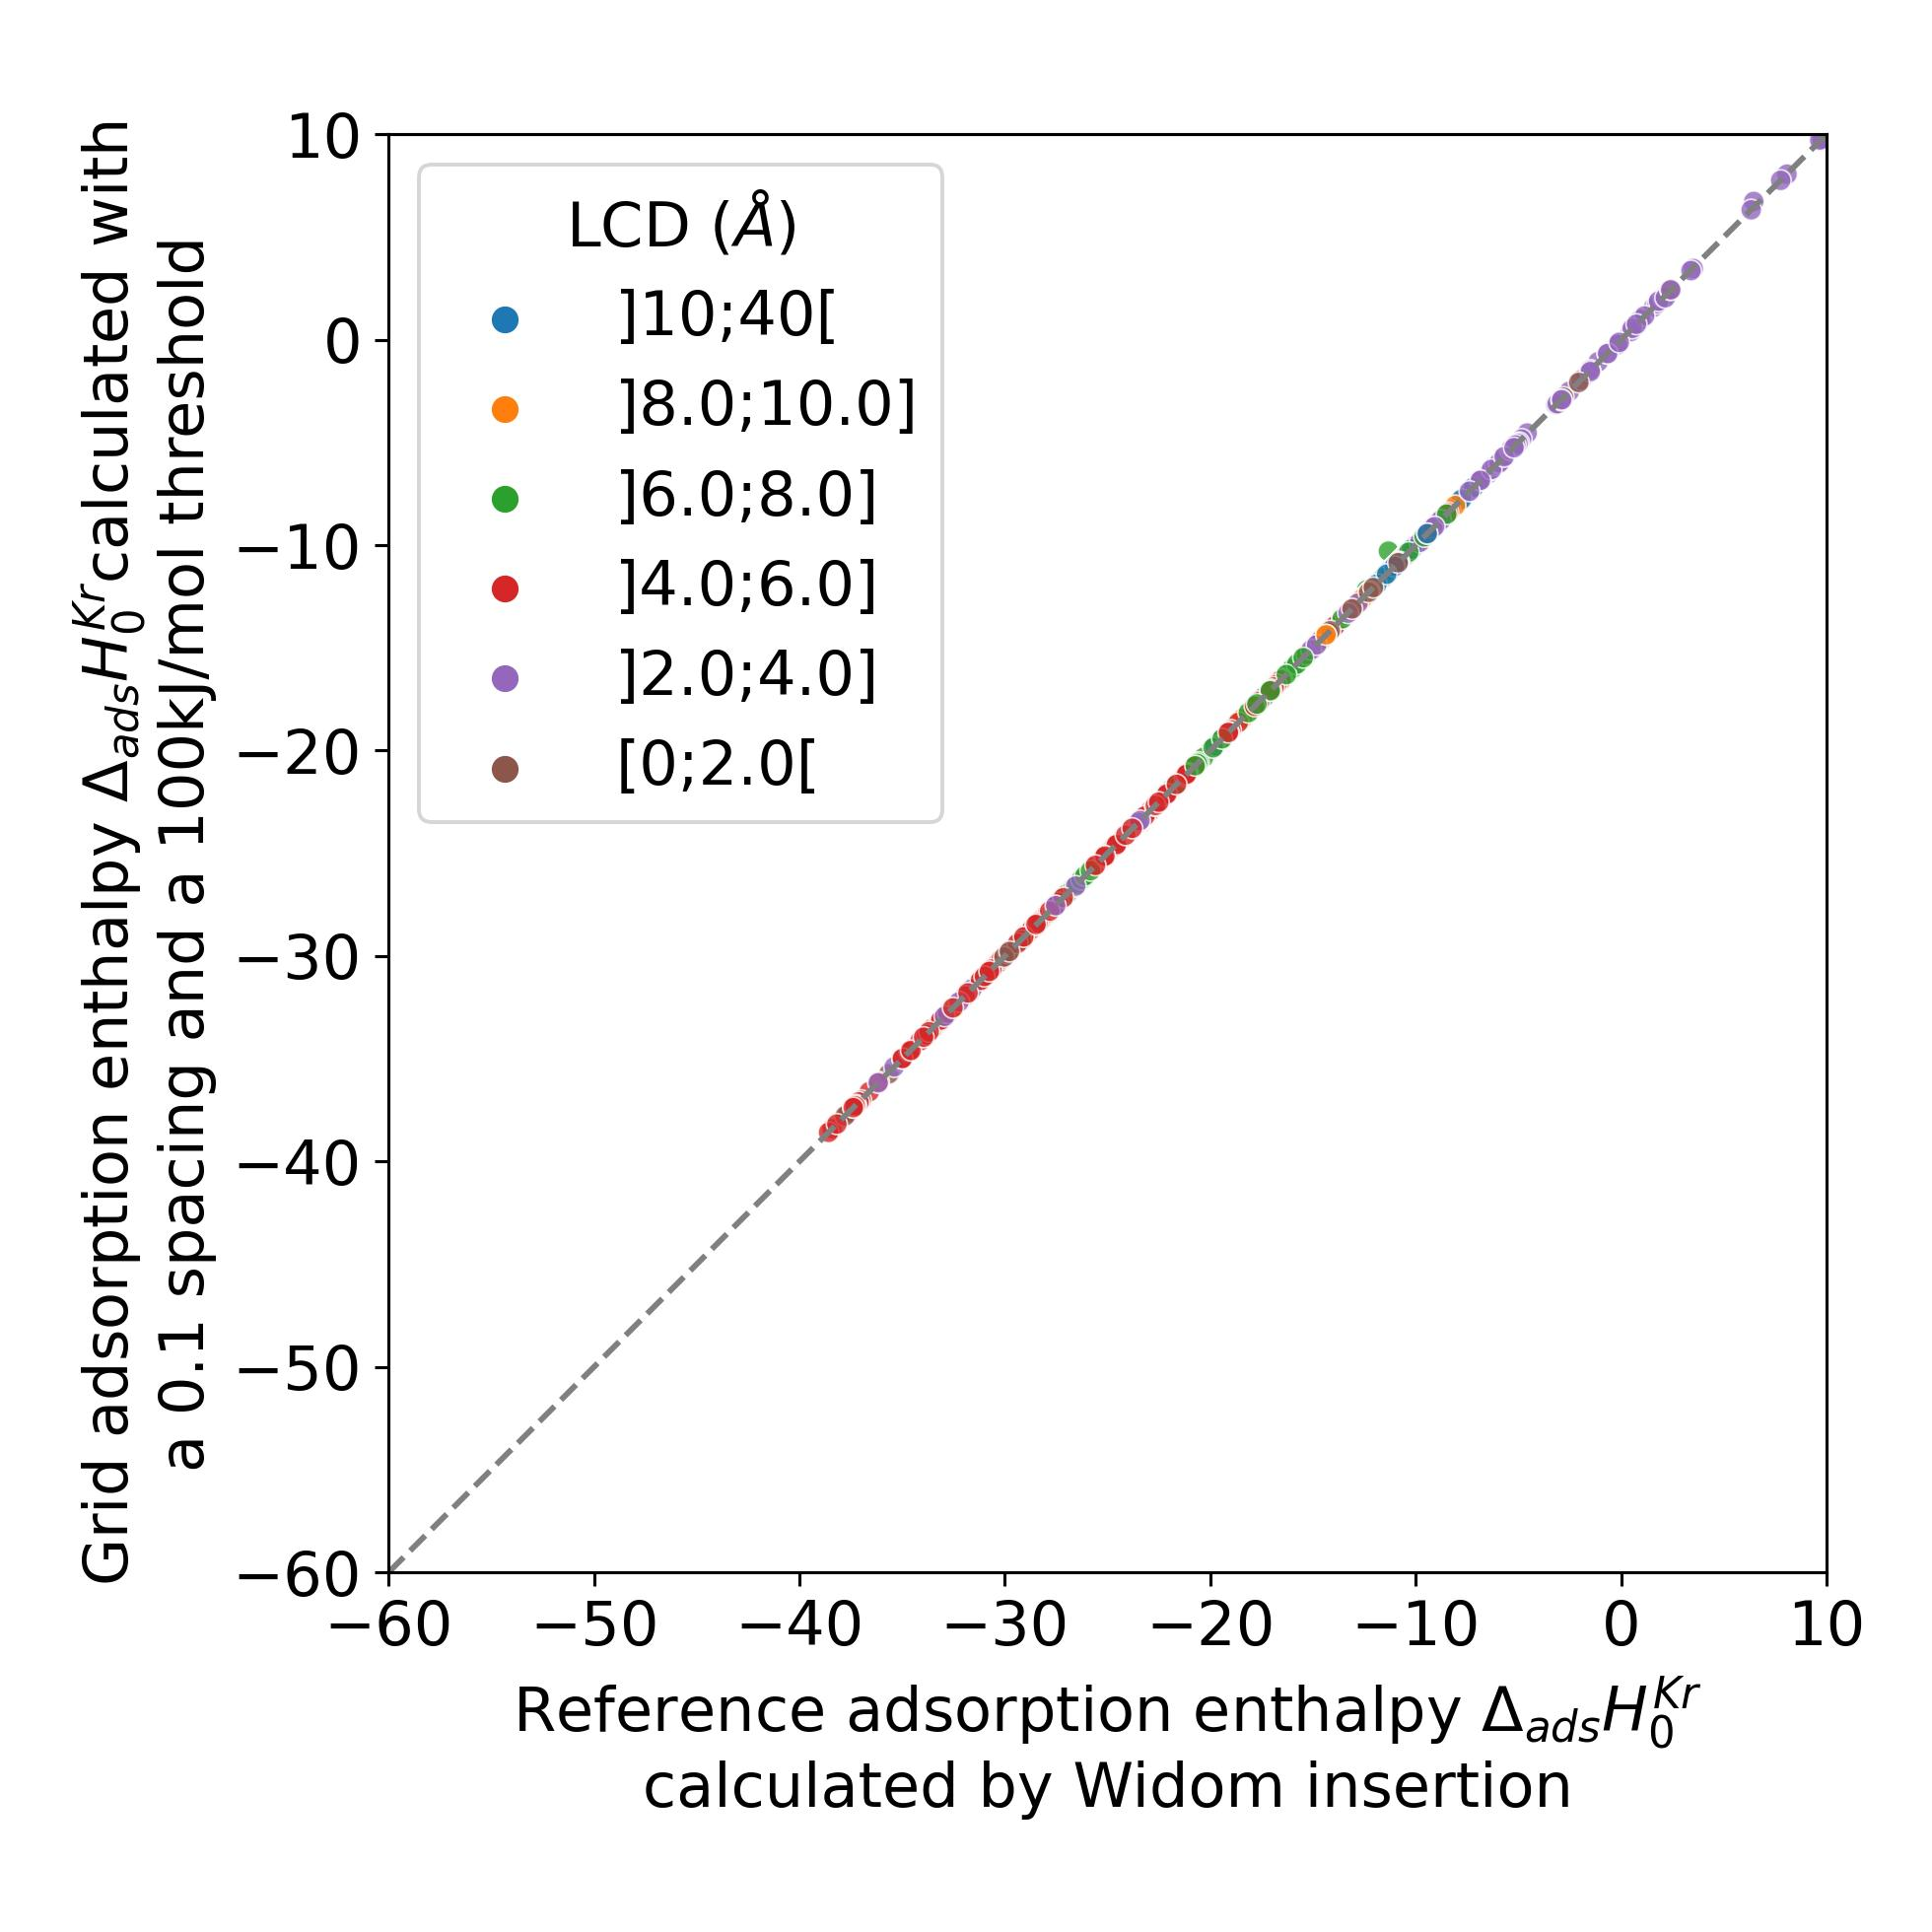
\includegraphics[width=0.45\textwidth]{figures/3-fastsim/H_Kr_0_widom_vs_H_Kr_grid_overview.jpg}
    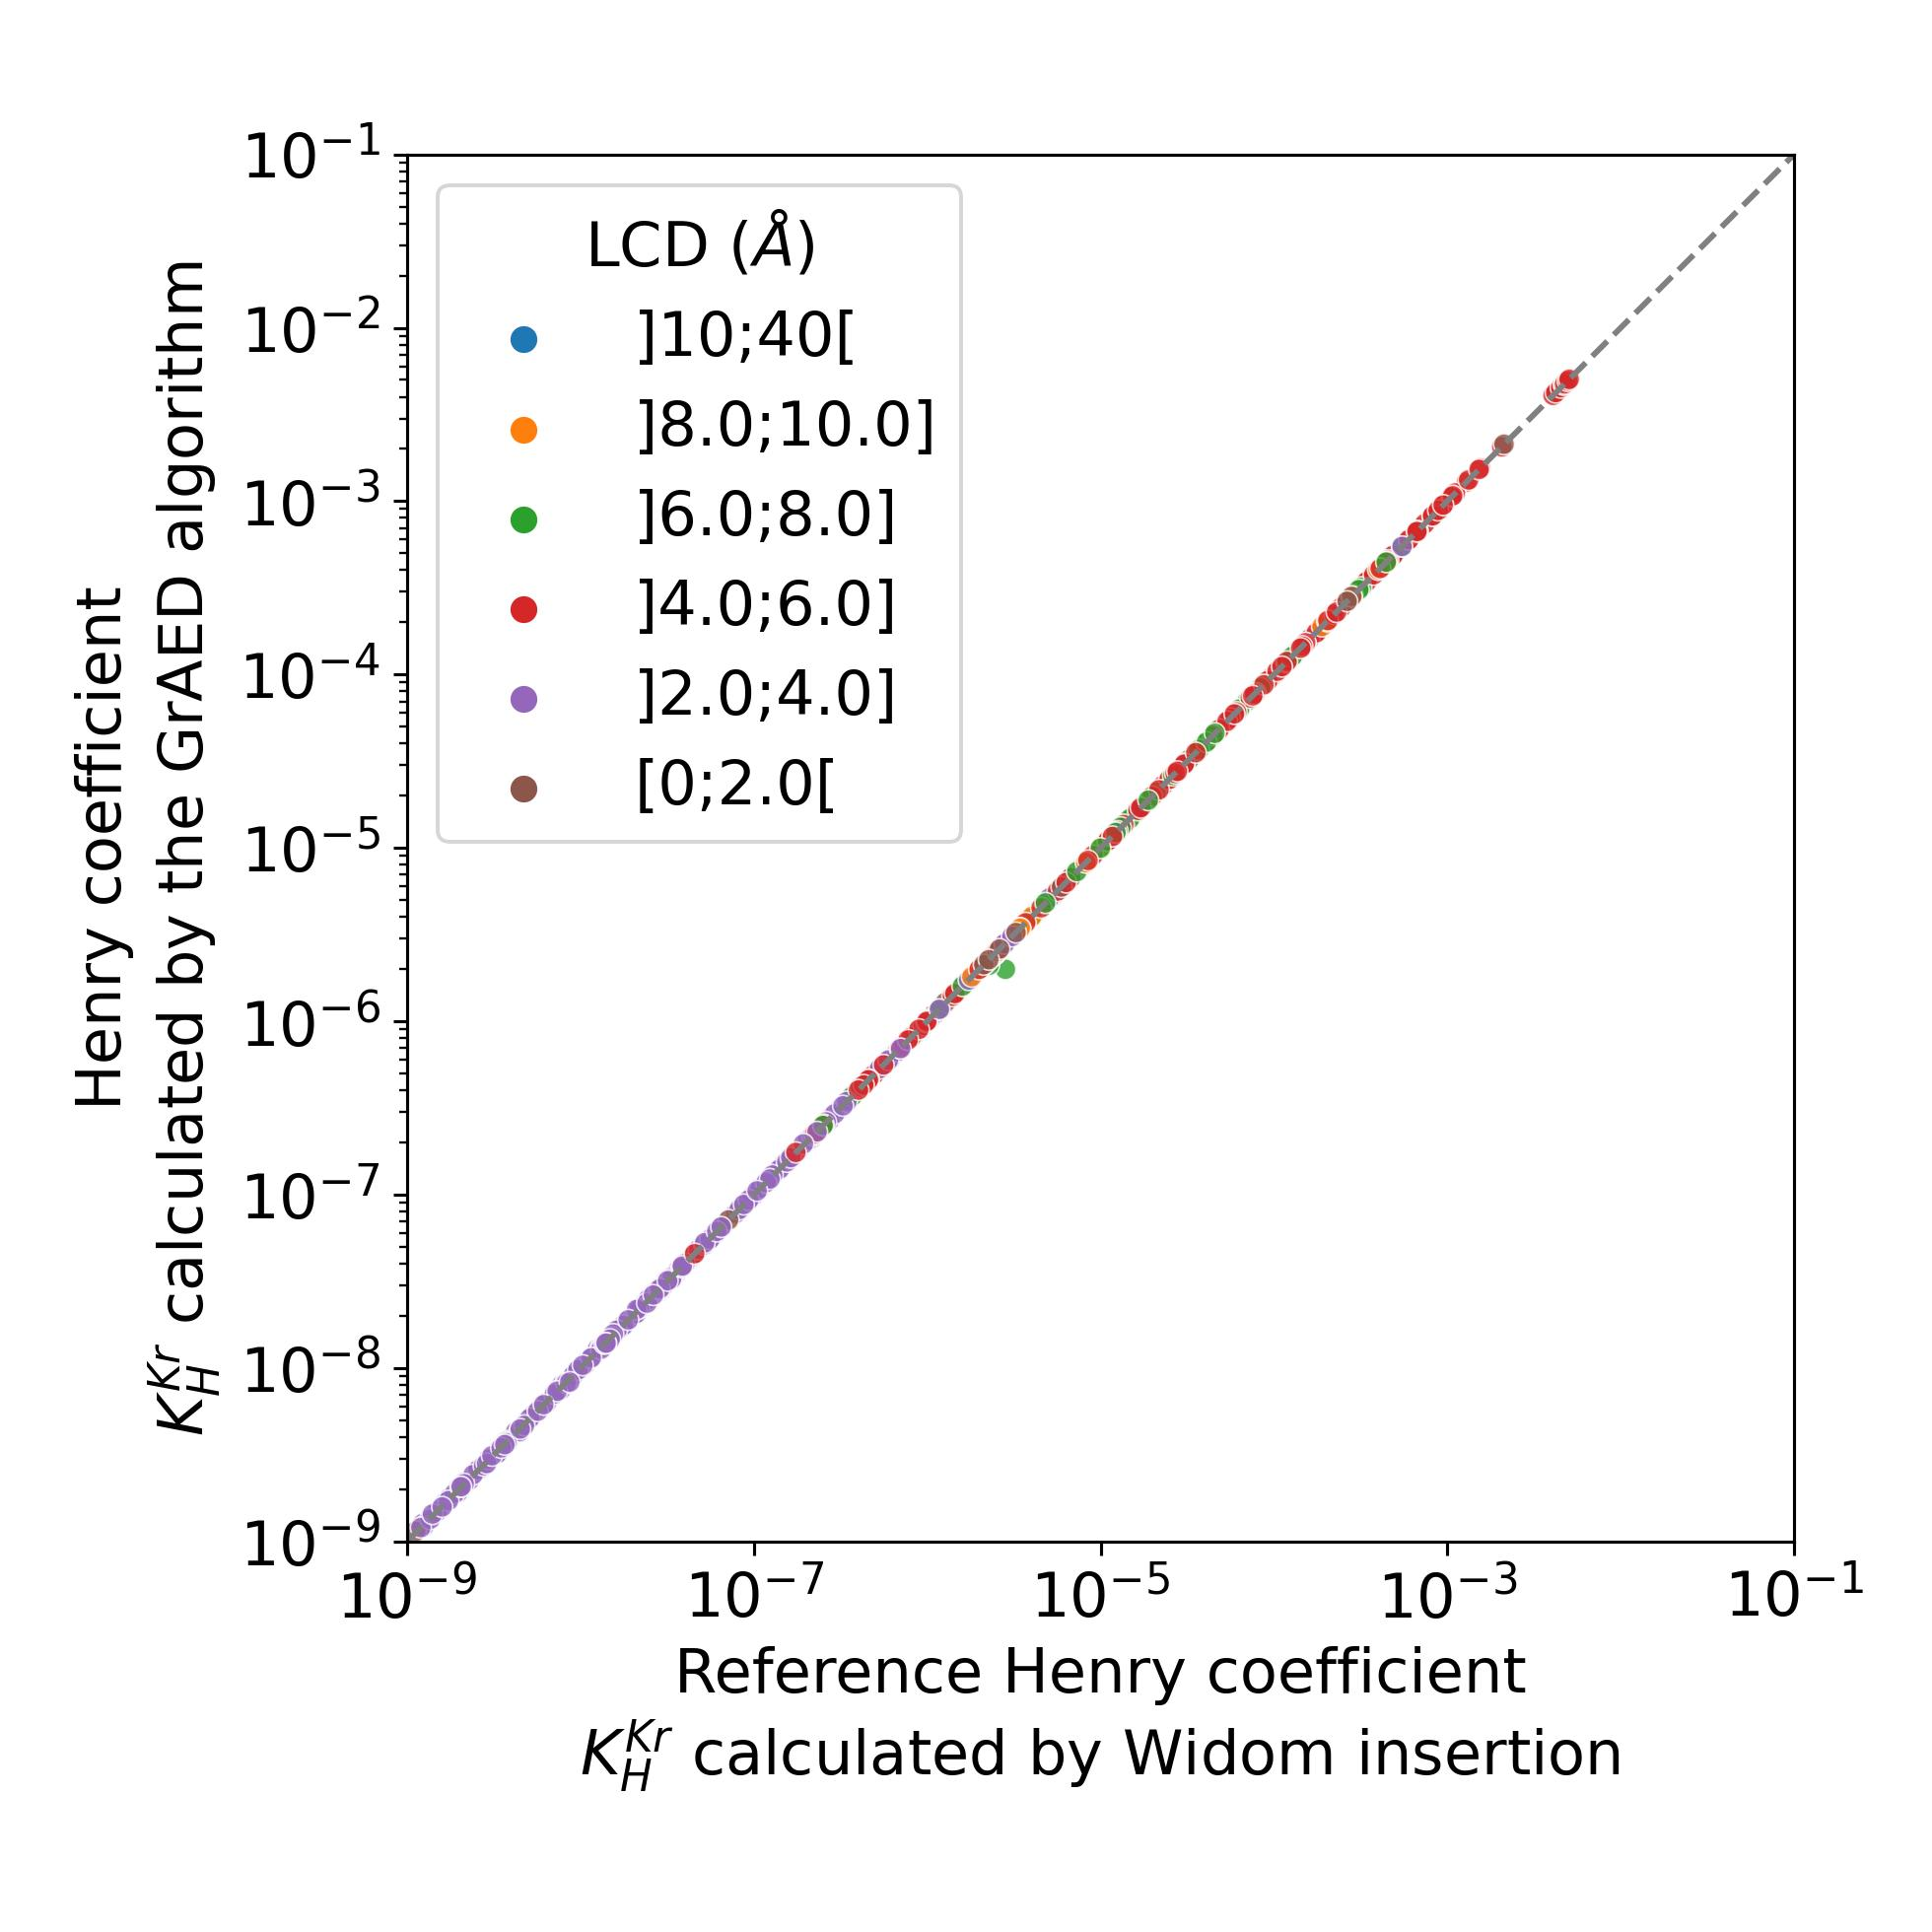
\includegraphics[width=0.45\textwidth]{figures/3-fastsim/K_Kr_widom_vs_K_Kr_grid_overview.jpg}
    \caption{Comparison of the krypton adsorption enthalpies (left) and the Henry constants (right) calculated by the optimized grid energy sampling (for a \SI{0.12}{\angstrom} spacing, a rejection parameter $\mu=0.8$ and an energy threshold $E\e{th}$ of \SI{100}{\kilo\joule\per\mole}) and by the Widom insertion of RASPA with 100,000 cycles. }\label{fgr:grid_widom_kr}
\end{figure}

First, we can start by looking at the adsorption properties of krypton calculated using the same grid spacing of \SI{0.12}{\angstrom}. The accuracy is more or less equivalent with an RMSE and an MAE on the krypton adsorption enthalpy of about \SI{0.02}{\kilo\joule\per\mole} and \SI{0.01}{\kilo\joule\per\mole}. As we can see on the Figure~\ref{fgr:grid_widom_kr}, the correlation is very strong for both the adsorption enthalpy (linear scale) and the Henry constant (log scale). The base 10 logarithm of the Henry constant (in \si{\milli\mole\per\gram\per\pascal}) has typically an RMSE of $0.002$, which is very similar to xenon. The relative error on the adsorption enthalpies of xenon and krypton does not go beyond {0.1\%} (values of the enthalpy have order of magnitude of dozens of \si{\kilo\joule\per\mole}), and the error on the xenon/krypton exchange enthalpy would therefore be very close to it. There is no reason for a huge impact on the exchange enthalpy. For the selectivity, we need to consider the relative error on the adsorption free energy which is a logarithmic transform of the Henry constant. We can estimate this relative error to around {0.2\%} (for a Henry constant of $10{-4}$~\si{\milli\mole\per\gram\per\pascal}), which also corresponds more or less to the relative error expected on the exchange Gibbs free energy or the log of the selectivity.

\begin{figure}[ht]
  \centering
    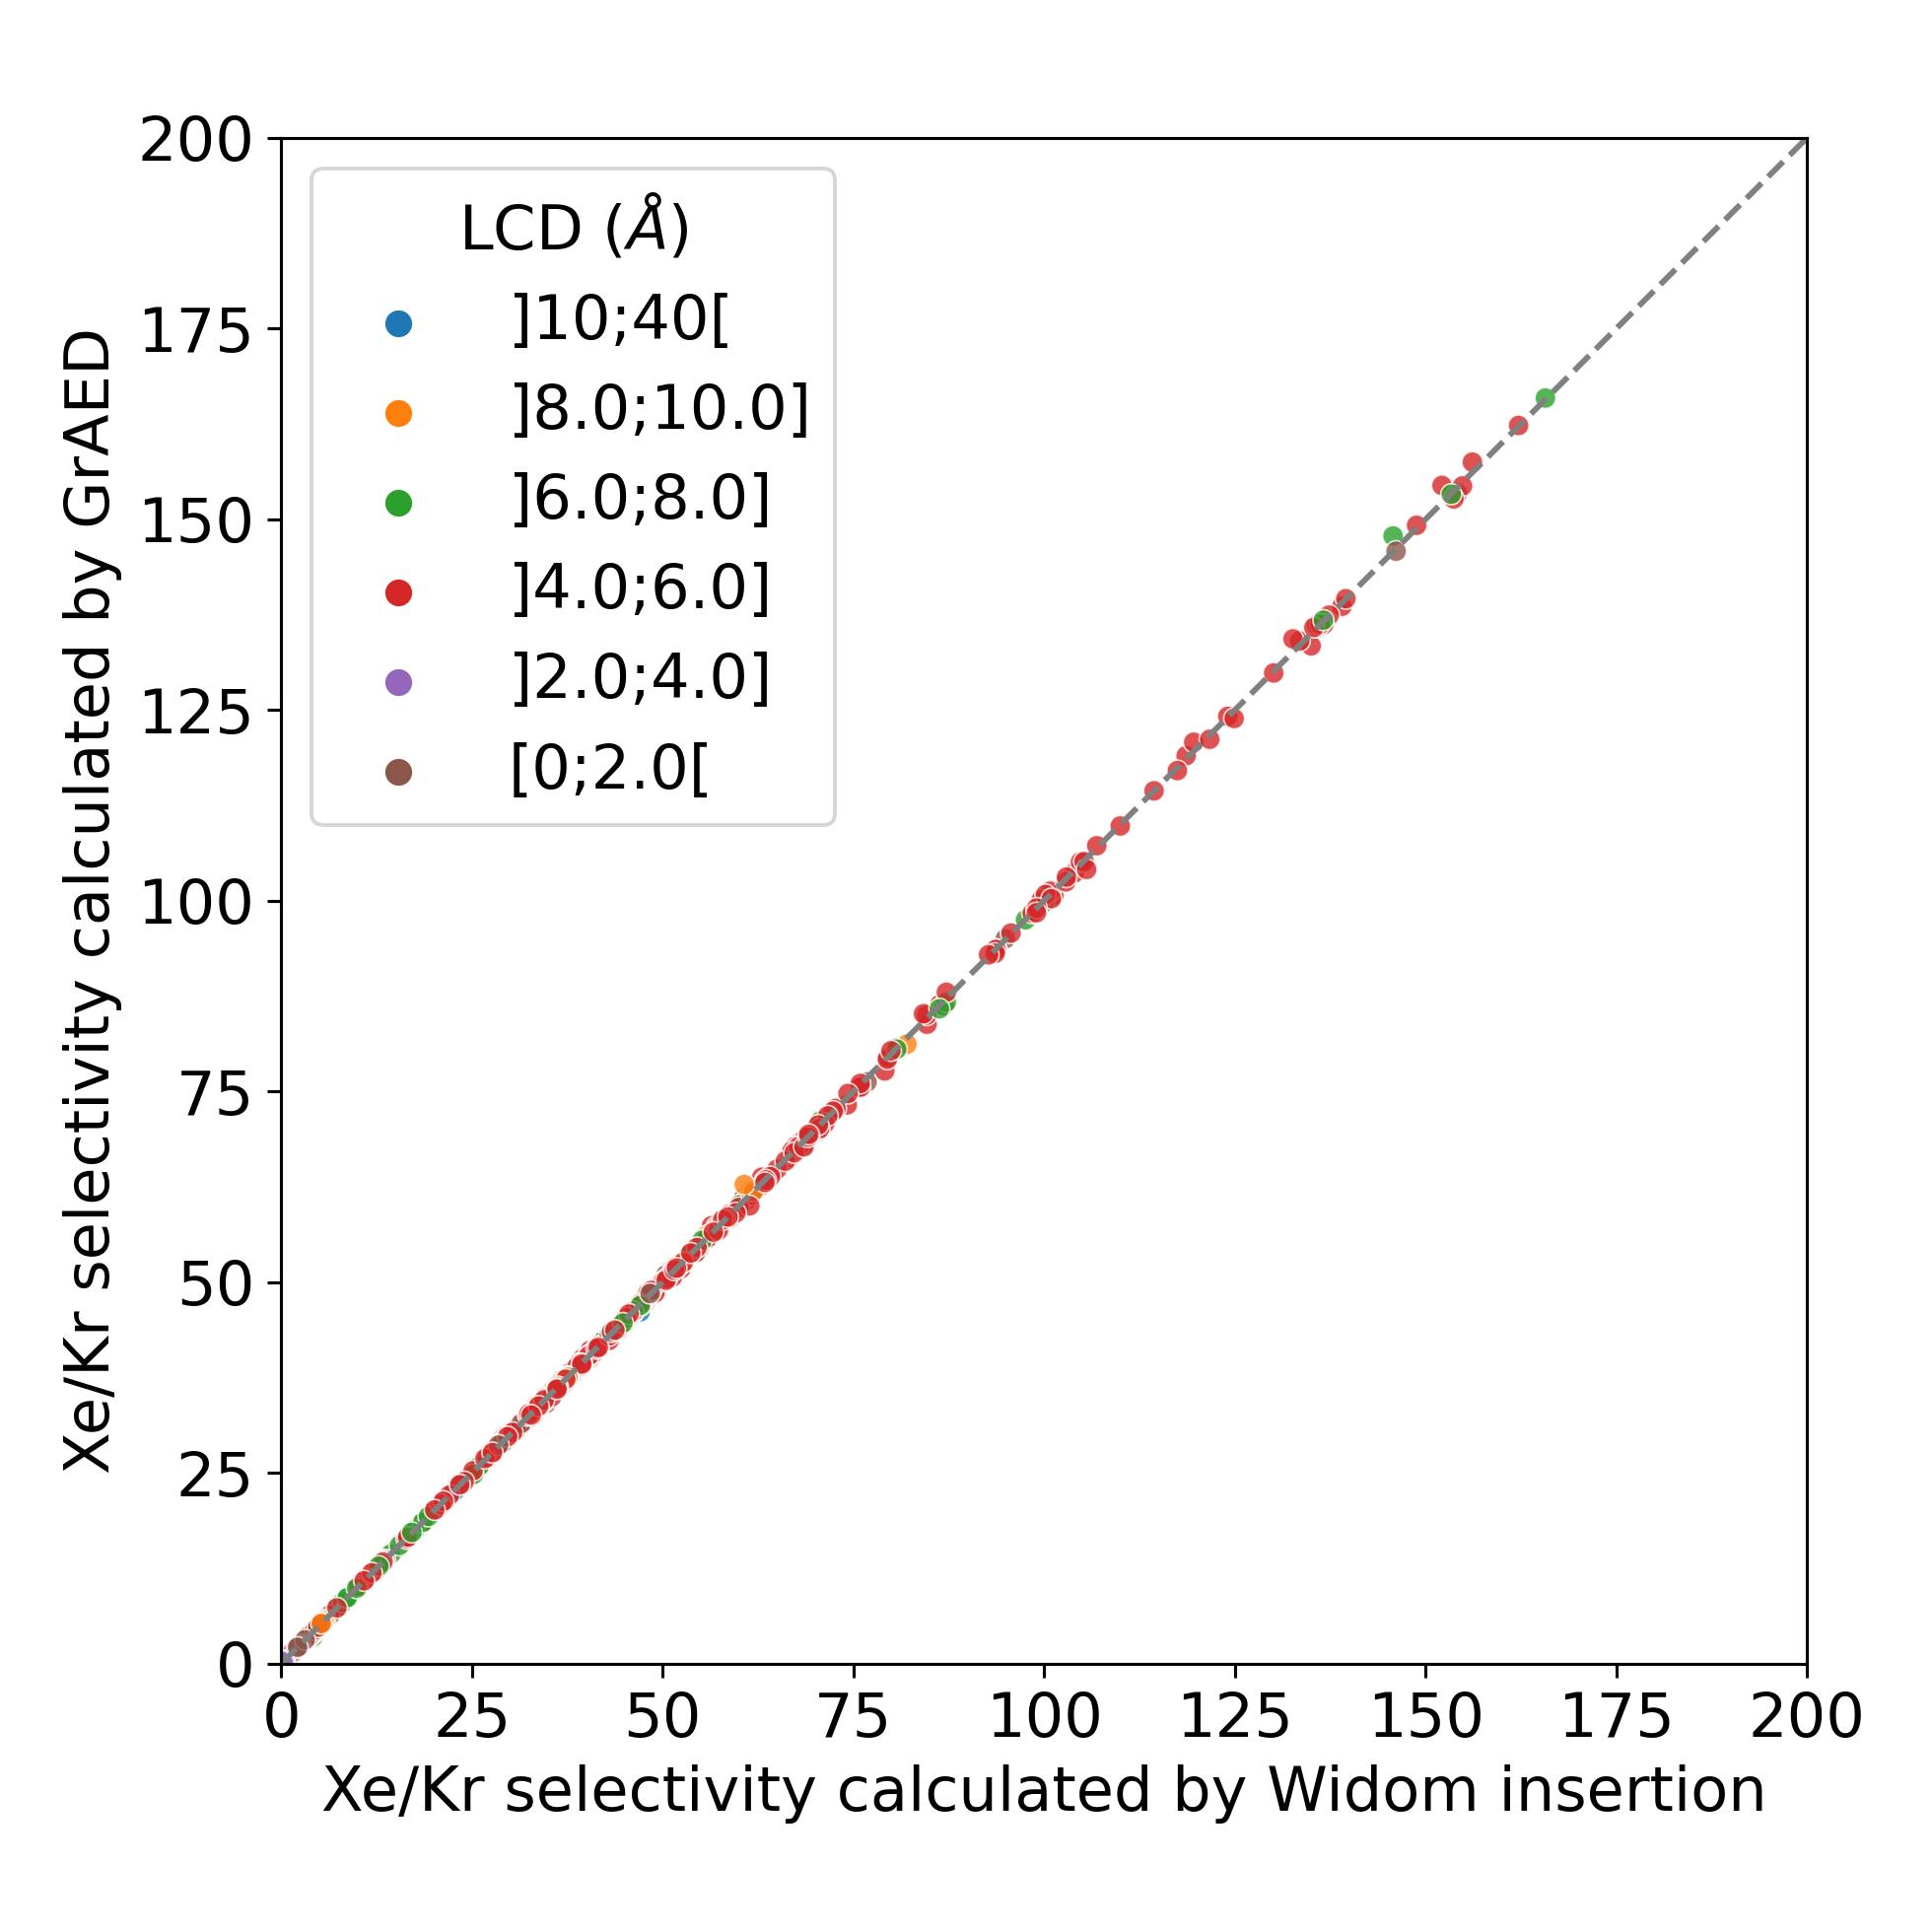
\includegraphics[width=0.45\textwidth]{figures/3-fastsim/s_0_widom_vs_s_0_grid_overview.jpg}
    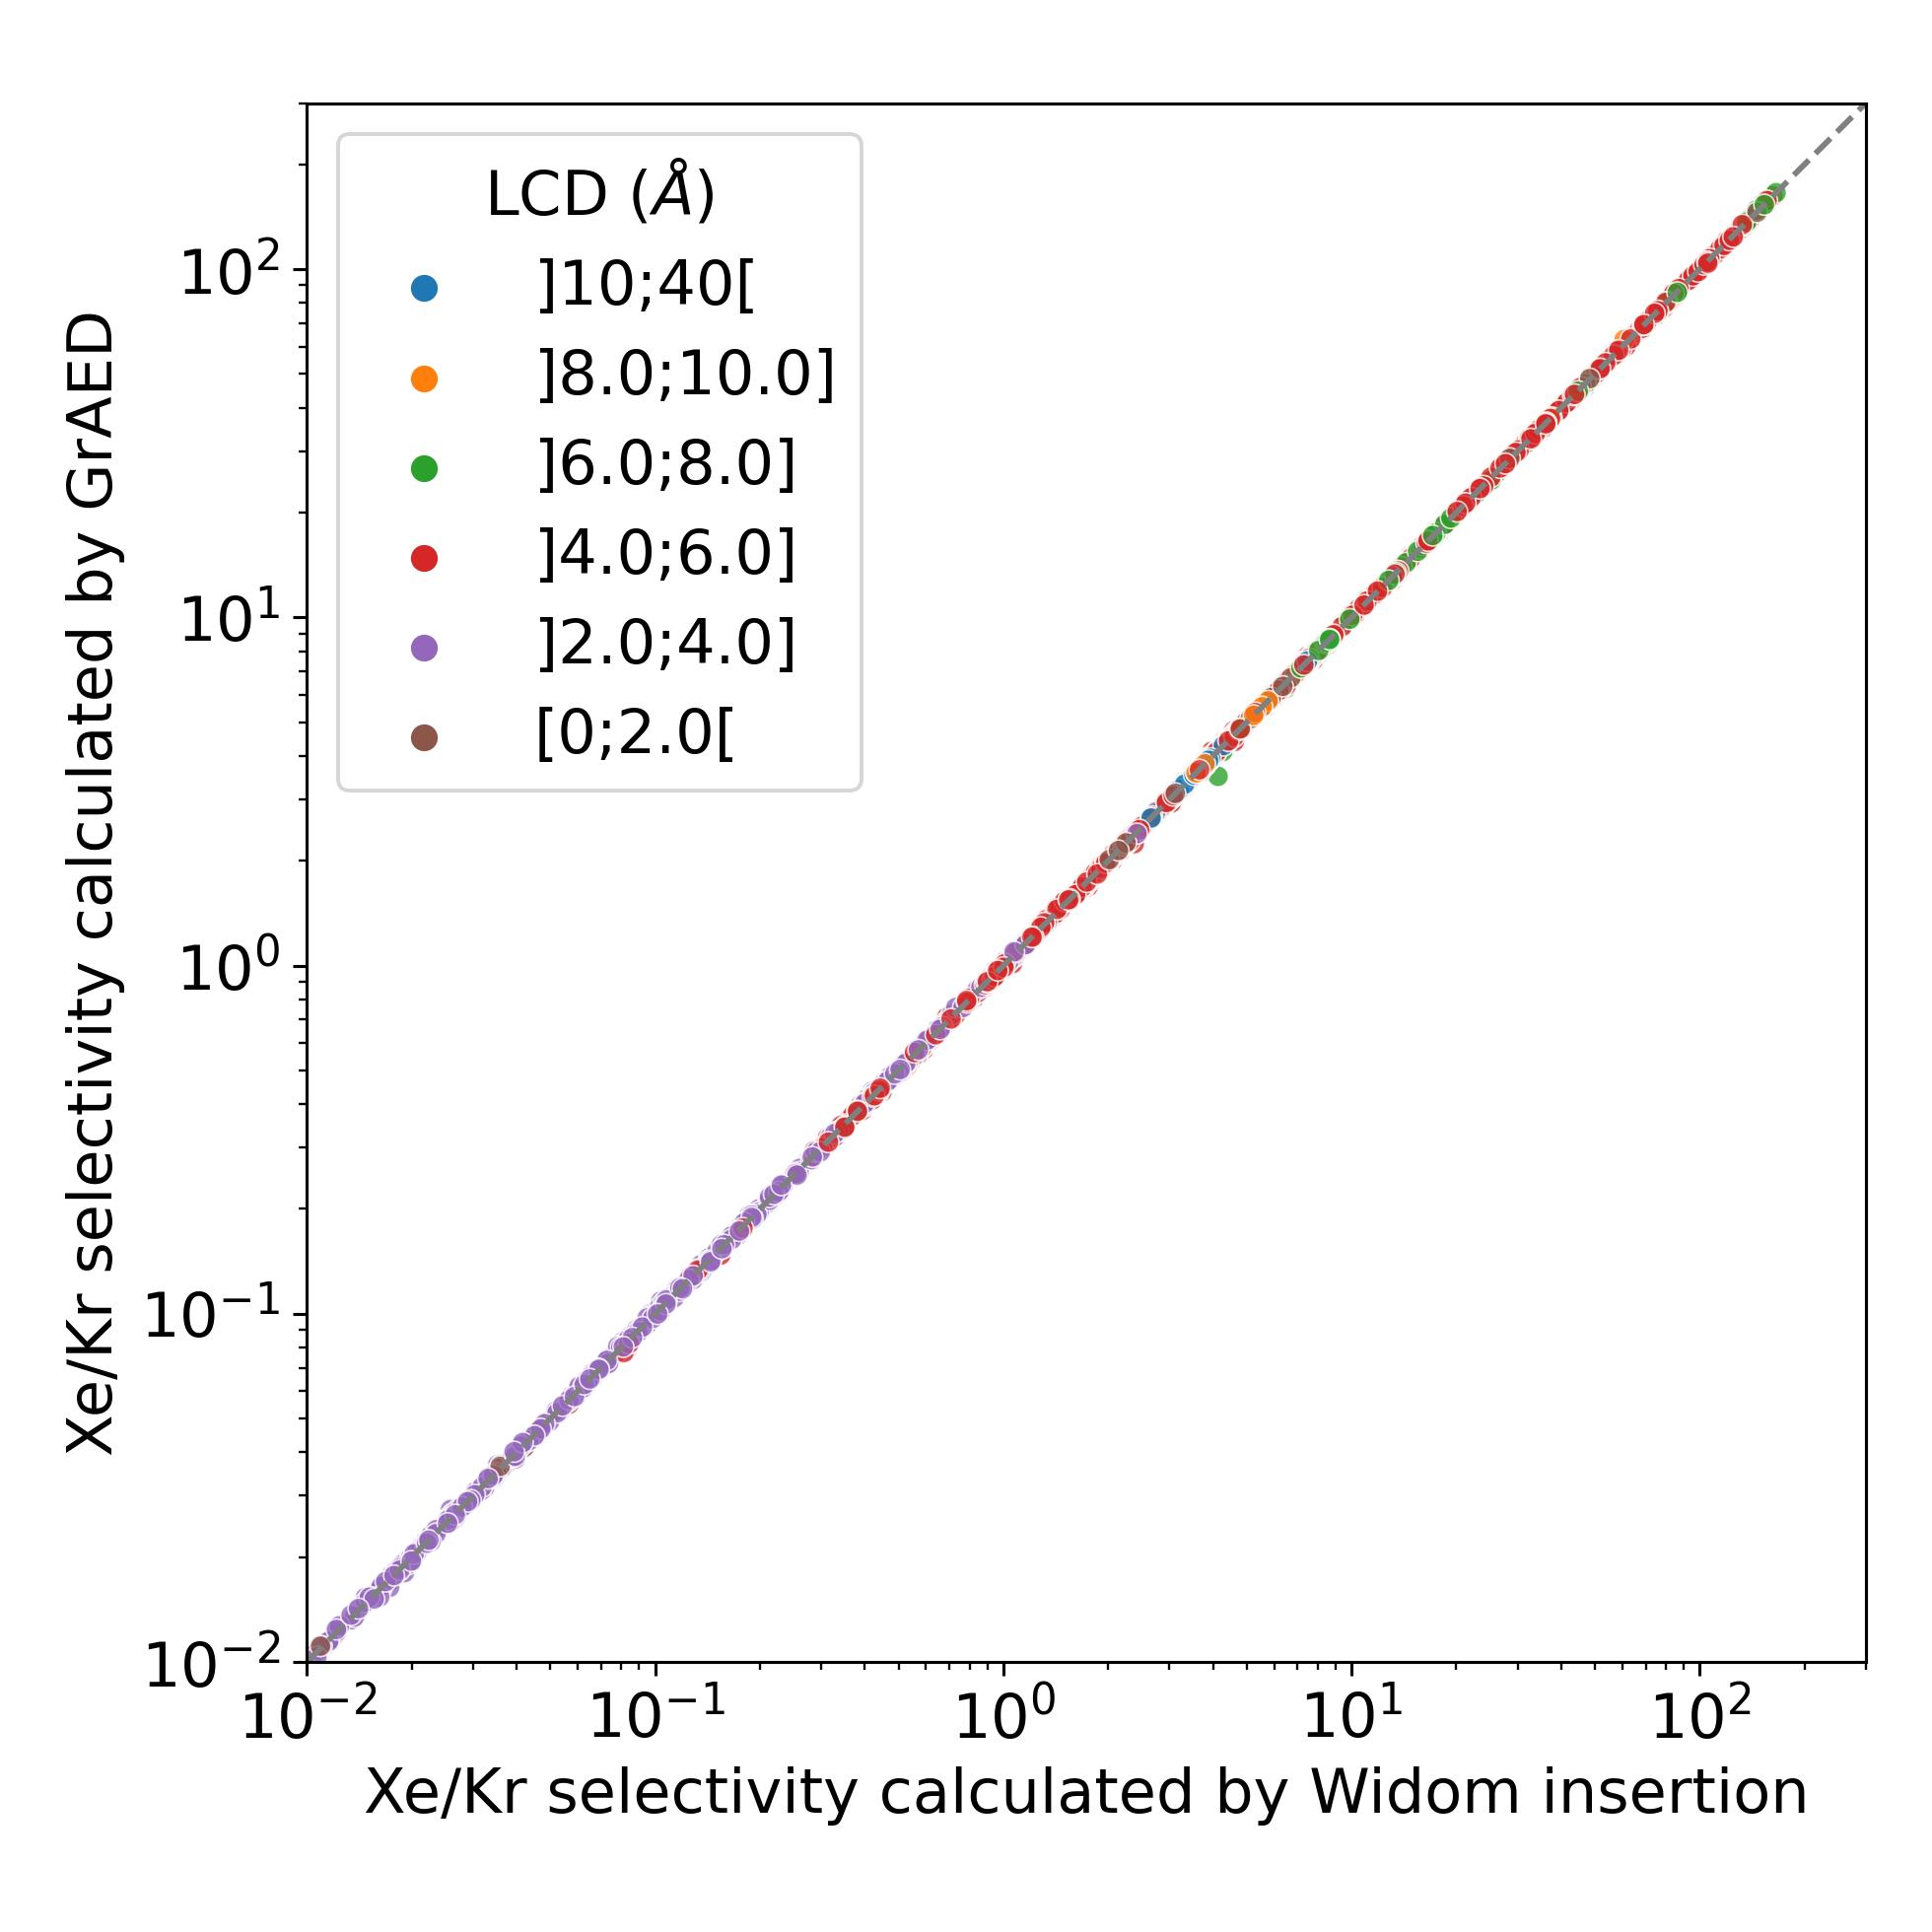
\includegraphics[width=0.45\textwidth]{figures/3-fastsim/s_0_widom_vs_s_0_grid_overview_log.jpg}
    \caption{Comparison of the Xe/Kr selectivity calculated by the optimized grid energy sampling (for a \SI{0.12}{\angstrom} spacing, a rejection parameter $\mu=0.8$ and an energy threshold $E\e{th}$ of \SI{100}{\kilo\joule\per\mole}) and by the Widom insertion of RASPA with 100,000 cycles. On the left, the axes are in linear scale, whereas the log scale has been used on the right. }\label{fgr:grid_widom_selectivity}
\end{figure}

If we now look at the Figure~\ref{fgr:grid_widom_selectivity}, the selectivity is as expected very well represented by the new grid sampling, especially for the logarithmic transform. The RMSE and the MAE on the selectivity values are actually of around $0.097$ and $0.035$, which is very low compared to the values of selectivity we are interested in (over $10$). For these selective structures, the relative error is actually below {0.1\%}. For base 10 logarithm of the selectivity or the exchange Gibbs free energy, the RMSE is around $0.014$, which means that we have a very good knowledge on the order of magnitude of the selectivity; if the selectivity were written in powers of ten, the exponent would be known at a precision of $\pm 0.014$.


The computation time required to compute the selectivity value of a structure of the CoRE MOF 2019 database is in average \SI{6.5}{\second}, since the krypton takes about \SI{3.5}{\second} to compute. If an algorithm computes both selectivity values at the same time, we can at least save the time required for initializing the software, which can marginally improve this time. This computation time required is still much lower than what we would need to compute two Widom insertions.

Now that we have proven the high accuracy and the efficiency of the GrAED algorithm for low-pressure selectivity evaluation, we will try to find relations between descriptors obtained using the grid-based algorithm and the selectivity at ambient pressure.

\subsection{Description of the ambient-pressure selectivity}

At first sight, if we look at the left plot of the Figure~\ref{fgr:grid_ambient_selectivity}, the selectivity at ambient pressure seems completely decorrelated to the selectivity at infinite dilution, which would mean that the sampling we have done is completely useless in determining the higher pressure selectivity values. However, the right plot suggests otherwise, the correlation between the logarithm of the selectivity does exist, the complete decorrelation we see at linear scale is actually a phenomenon that only occurs on highly selective materials. This phenomenon is described in detail in the chapter 2 and corresponds to a selectivity drop experienced by some highly (at infinite dilution) selective materials. To say it simply, the saturation of the most selective sites make the remaining sites way less selective for the xenon/krypton separation for these materials.

\begin{figure}[ht]
  \centering
    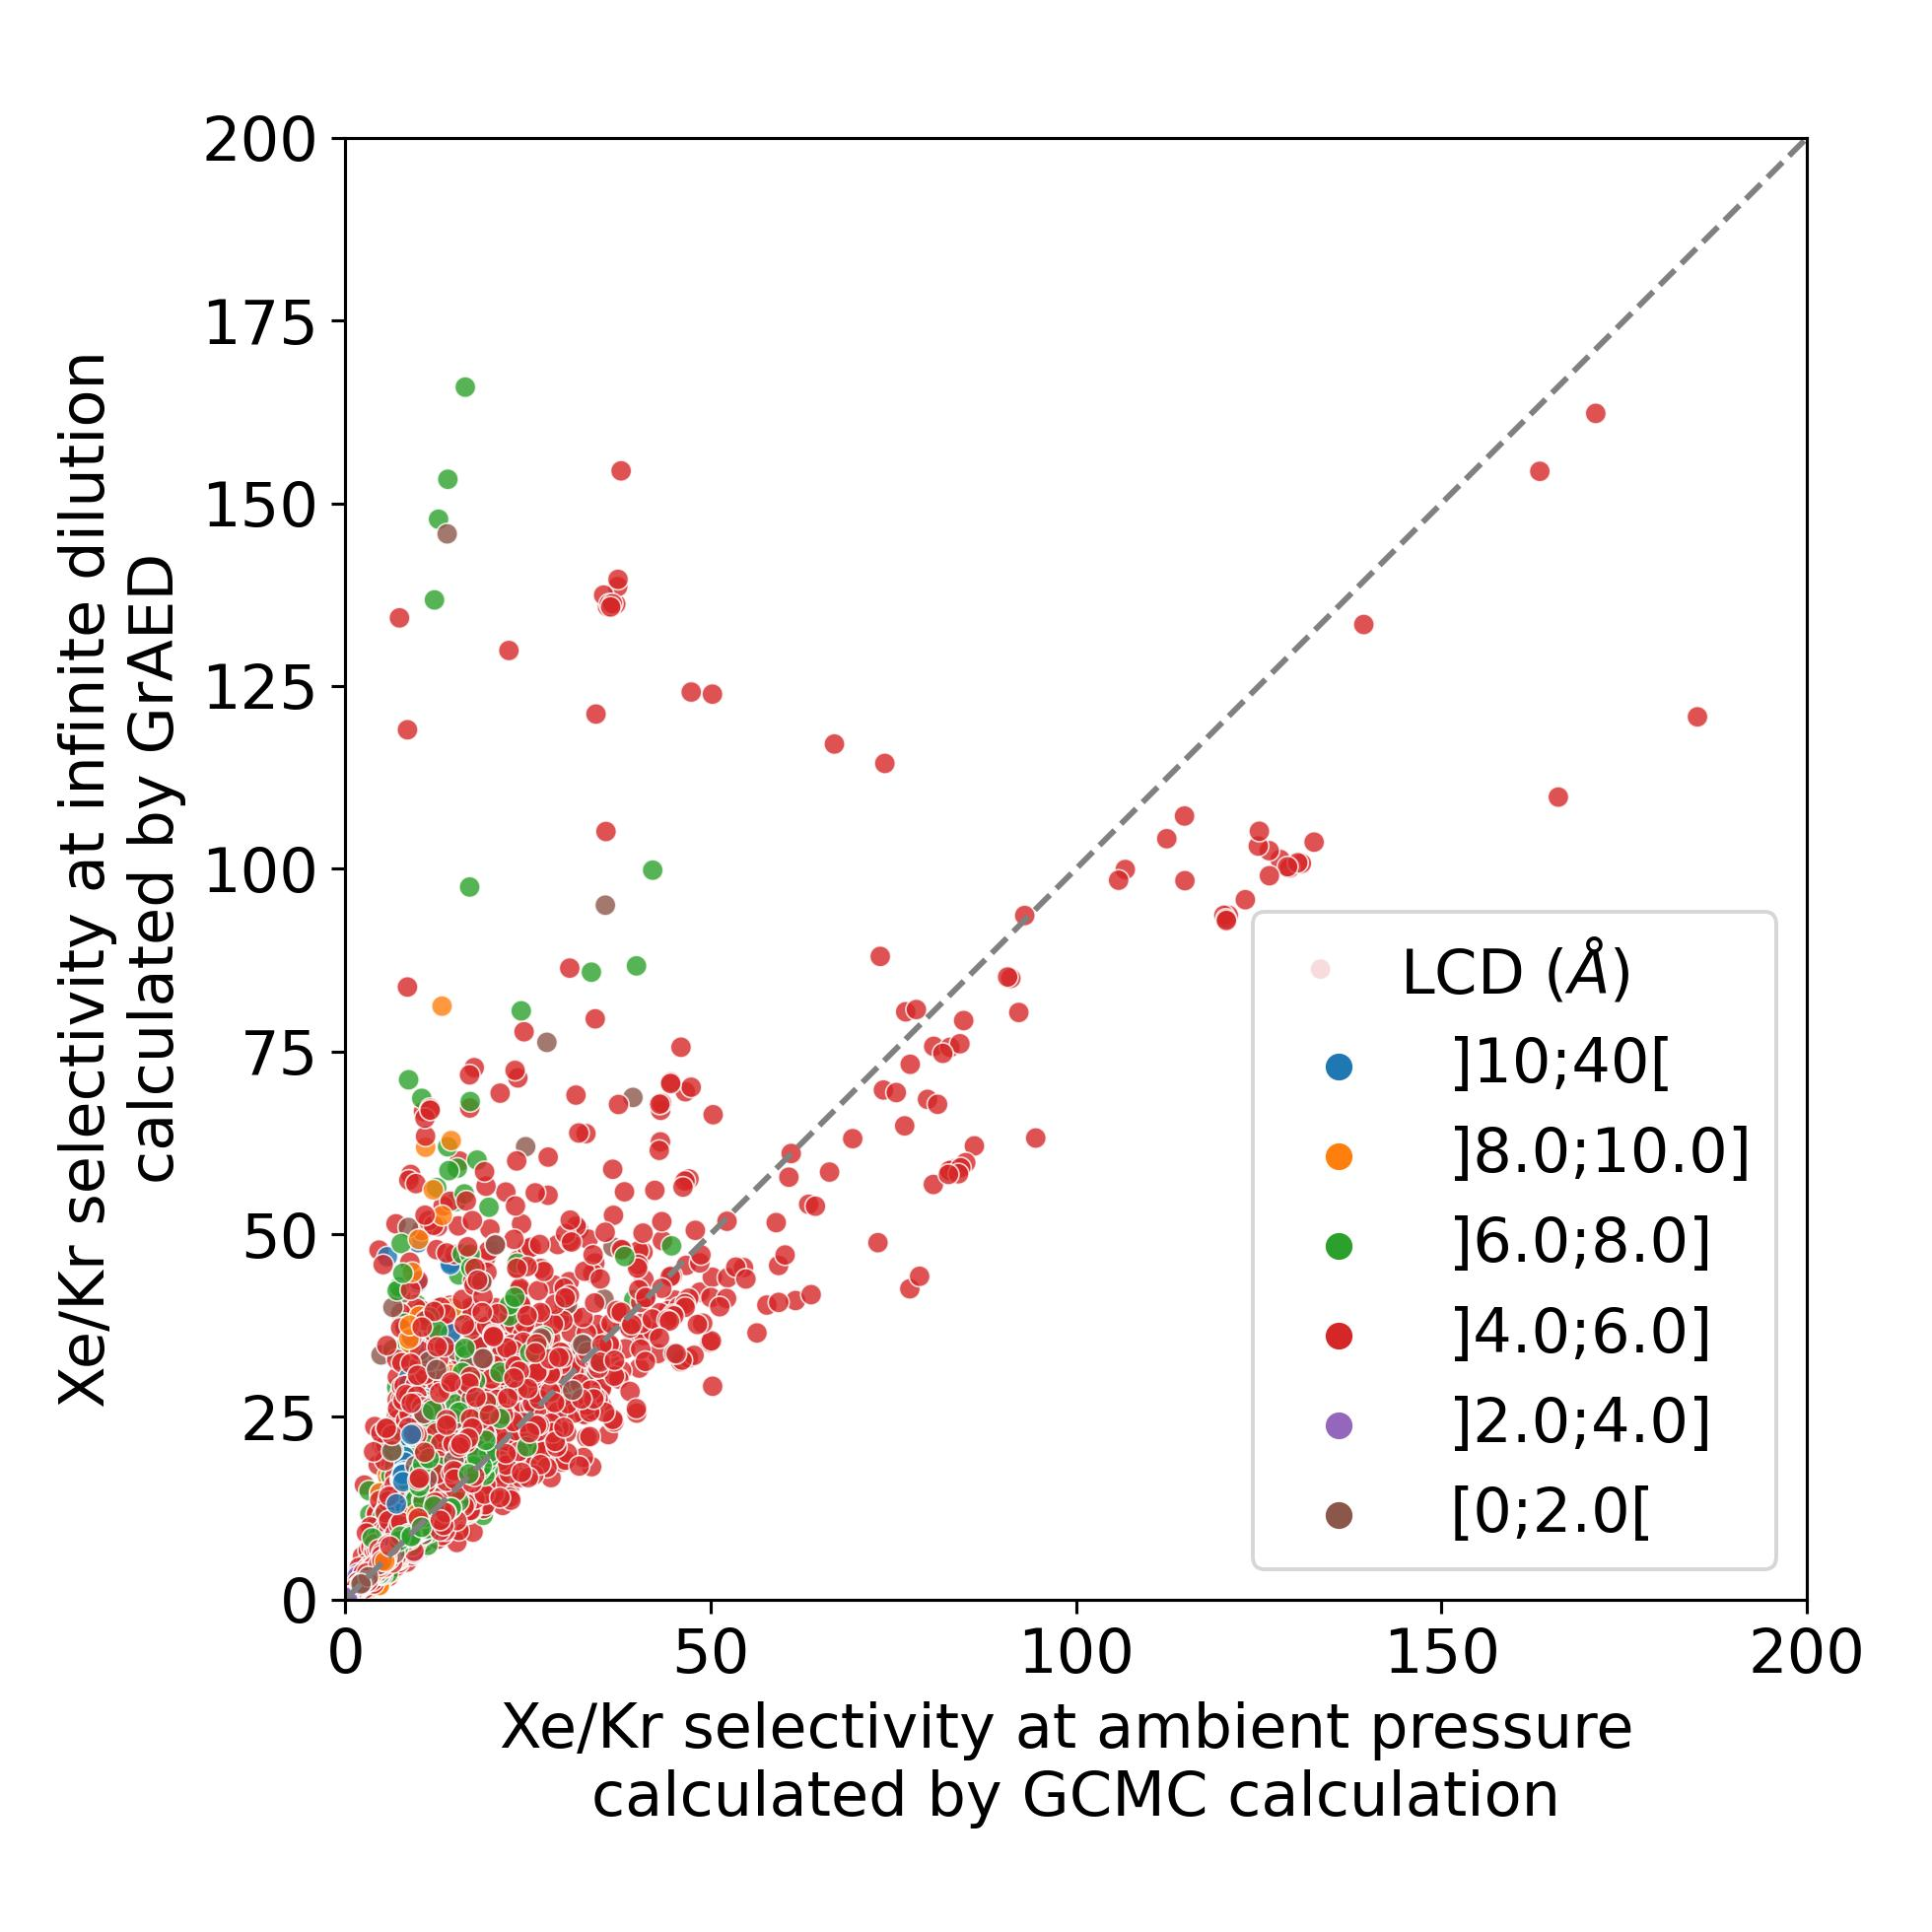
\includegraphics[width=0.45\textwidth]{figures/3-fastsim/s_2080_vs_s_0_grid_overview.jpg}
    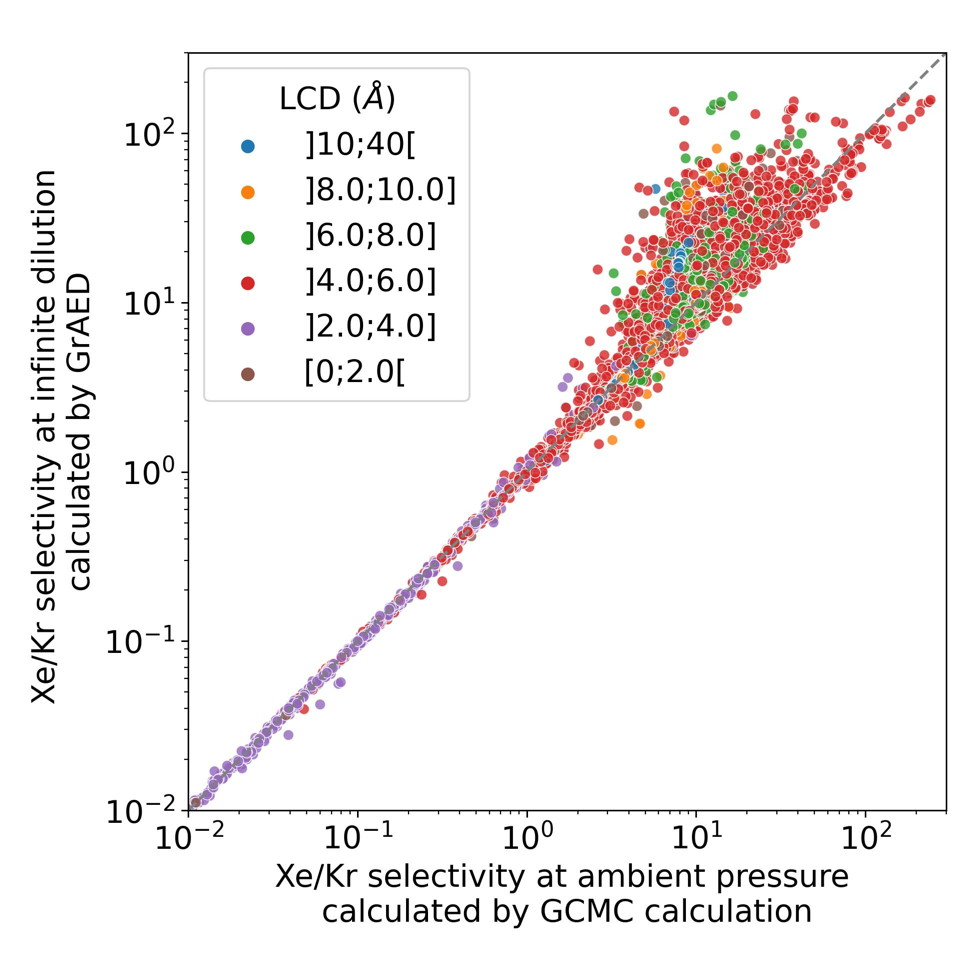
\includegraphics[width=0.45\textwidth]{figures/3-fastsim/s_2080_vs_s_0_grid_overview_log.jpg}
    \caption{Comparison of the low-pressure Xe/Kr selectivity calculated by the GrAED algorithm (same parameters) and the ambient-pressure selectivity calculated by GCMC simulations of RASPA with 100,000 cycles. On the left, the axes are in linear scale, whereas the log scale has been used on the right. }\label{fgr:grid_ambient_selectivity}
\end{figure}

The goal is then to be able to design descriptors that could help distinguish this selectivity dropping materials with the materials keeping their high selectivity at higher pressure. We propose three concepts that could help better understand the origin of this drop of selectivity at higher pressure: (1) other adsorption thermodynamic quantities, (2) higher temperature averaging can also be a good proxy to understand higher pressure adsorption, and (3) statistical quantities derived from the energy distributions. All of these descriptors can be obtained through a grid sampling; however, one should note that the guest--guest interactions that occur at higher pressure cannot be captured by this method.


\subsubsection{Thermodynamic quantities}

As we saw in the previous chapter, many thermodynamic quantities can be calculated at infinite dilution: adsorption and exchange Gibbs free energies, enthalpies and entropies. If we consider the xenon and krypton separation, we can generate 9 different descriptors. We will look at the relation between these quantities and the high-pressure selectivity values. In the introduction, we already tackled the relation between the exchange Gibbs free energy, since it is the logarithmic transform of the infinite dilution selectivity plotted on the Figure~\ref{fgr:grid_ambient_selectivity}. This quantity is the most important descriptor as it sets an initial reference value to understand the problem. The selectivity at high pressure can be seen as the selectivity at infinite dilution plus or minus a shift due to the specificity of the adsorption at higher pressure in a given material.


\begin{figure}[ht]
  \centering
    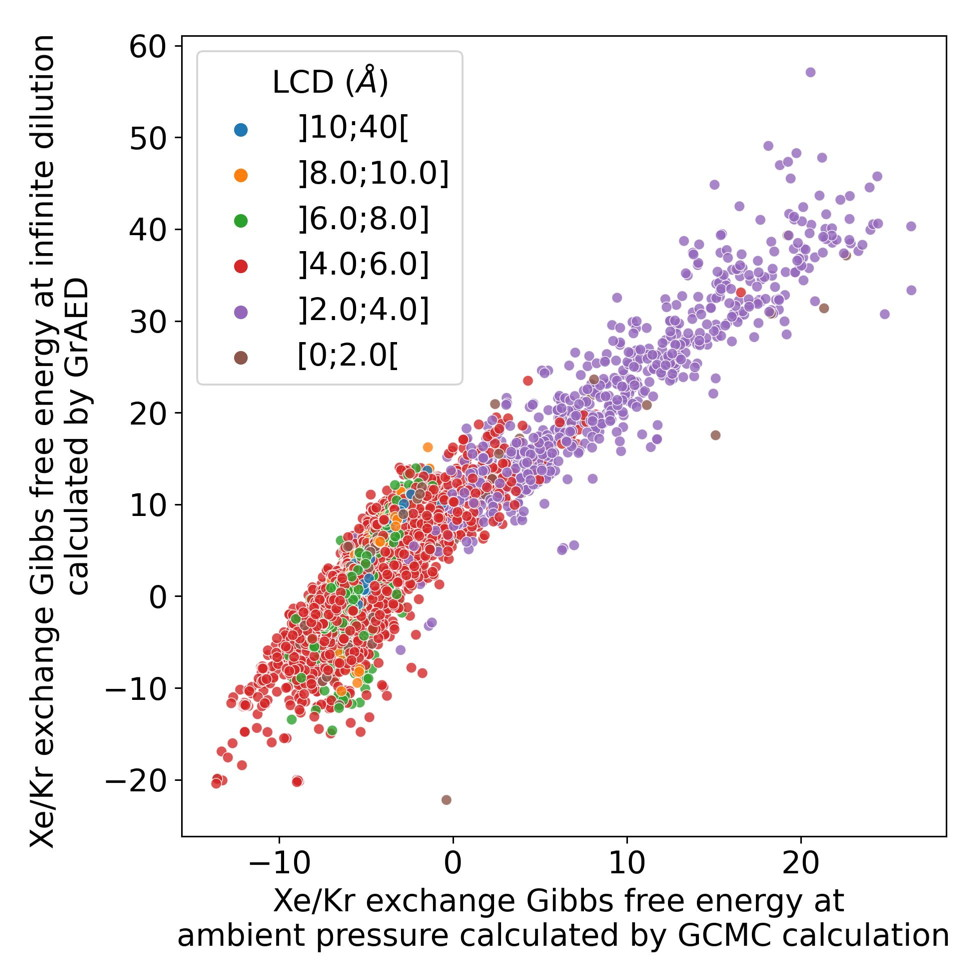
\includegraphics[width=0.45\textwidth]{figures/3-fastsim/G_2080_vs_G_Xe_grid_overview.jpg}
    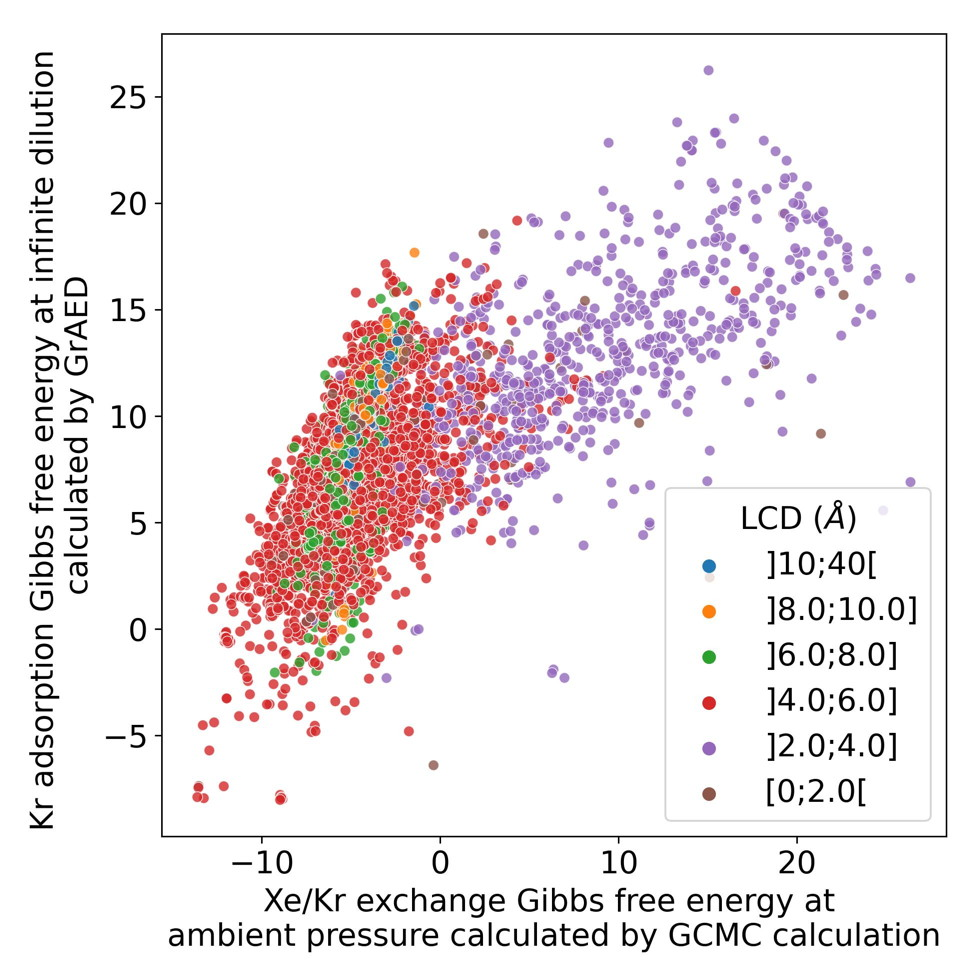
\includegraphics[width=0.45\textwidth]{figures/3-fastsim/G_2080_vs_G_Kr_grid_overview.jpg}
    \caption{Comparison of the ambient-pressure Xe/Kr exchange Gibbs free energy calculated by GCMC simulations of RASPA with 100,000 cycles and the low-pressure adsorption free energies of xenon (left) and krypton (right) in \si{\kilo\joule\per\mole} calculated by the GrAED algorithm (same parameters).}\label{fgr:grid_comp_gibbs}
\end{figure}

Without any surprise, the Figure\ref{fgr:grid_comp_gibbs} confirms that a good adsorption of xenon is a good indication for the efficiency of the separation from krypton since we have a very strong correlation between the Xe/Kr exchange Gibbs free energy and the xenon adsorption Gibbs free energy. The correlation with the xenon adsorption Gibbs free energy is very weak and still positive, this means that a good material for the Xe/Kr separation would not be very bad for krypton adsorption but rather pretty average. Put differently, it is not possible to find a material very good for xenon adsorption and very bad for krypton, which explains an apparent theoretical limitation to the selectivity theoretically capped under $200$ (in our level of theory for materials of CoRE MOF 2019, of course, see Figure~\ref{fgr:grid_widom_selectivity} and~\ref{fgr:grid_ambient_selectivity}). Experimentally, no material has exceeded a selectivity value of $100$.

\begin{figure}[ht]
  \centering
    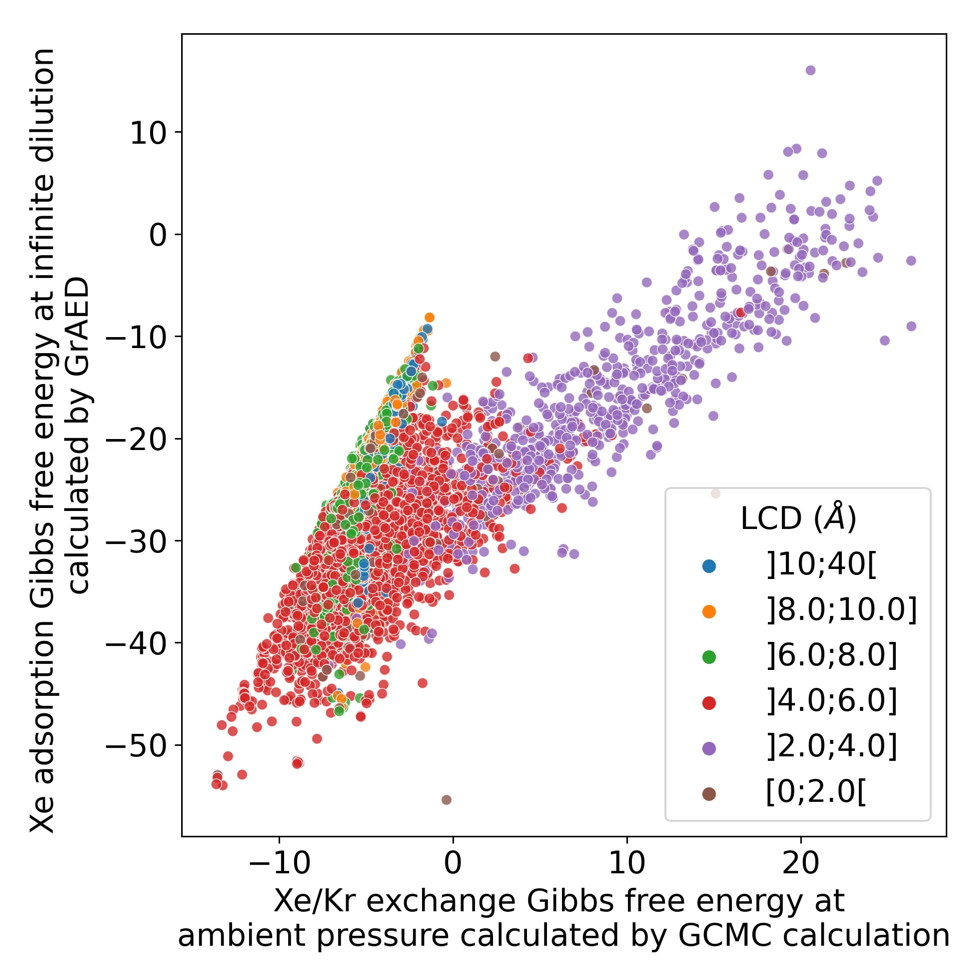
\includegraphics[width=0.45\textwidth]{figures/3-fastsim/G_2080_vs_H_Xe_grid_overview.jpg}
    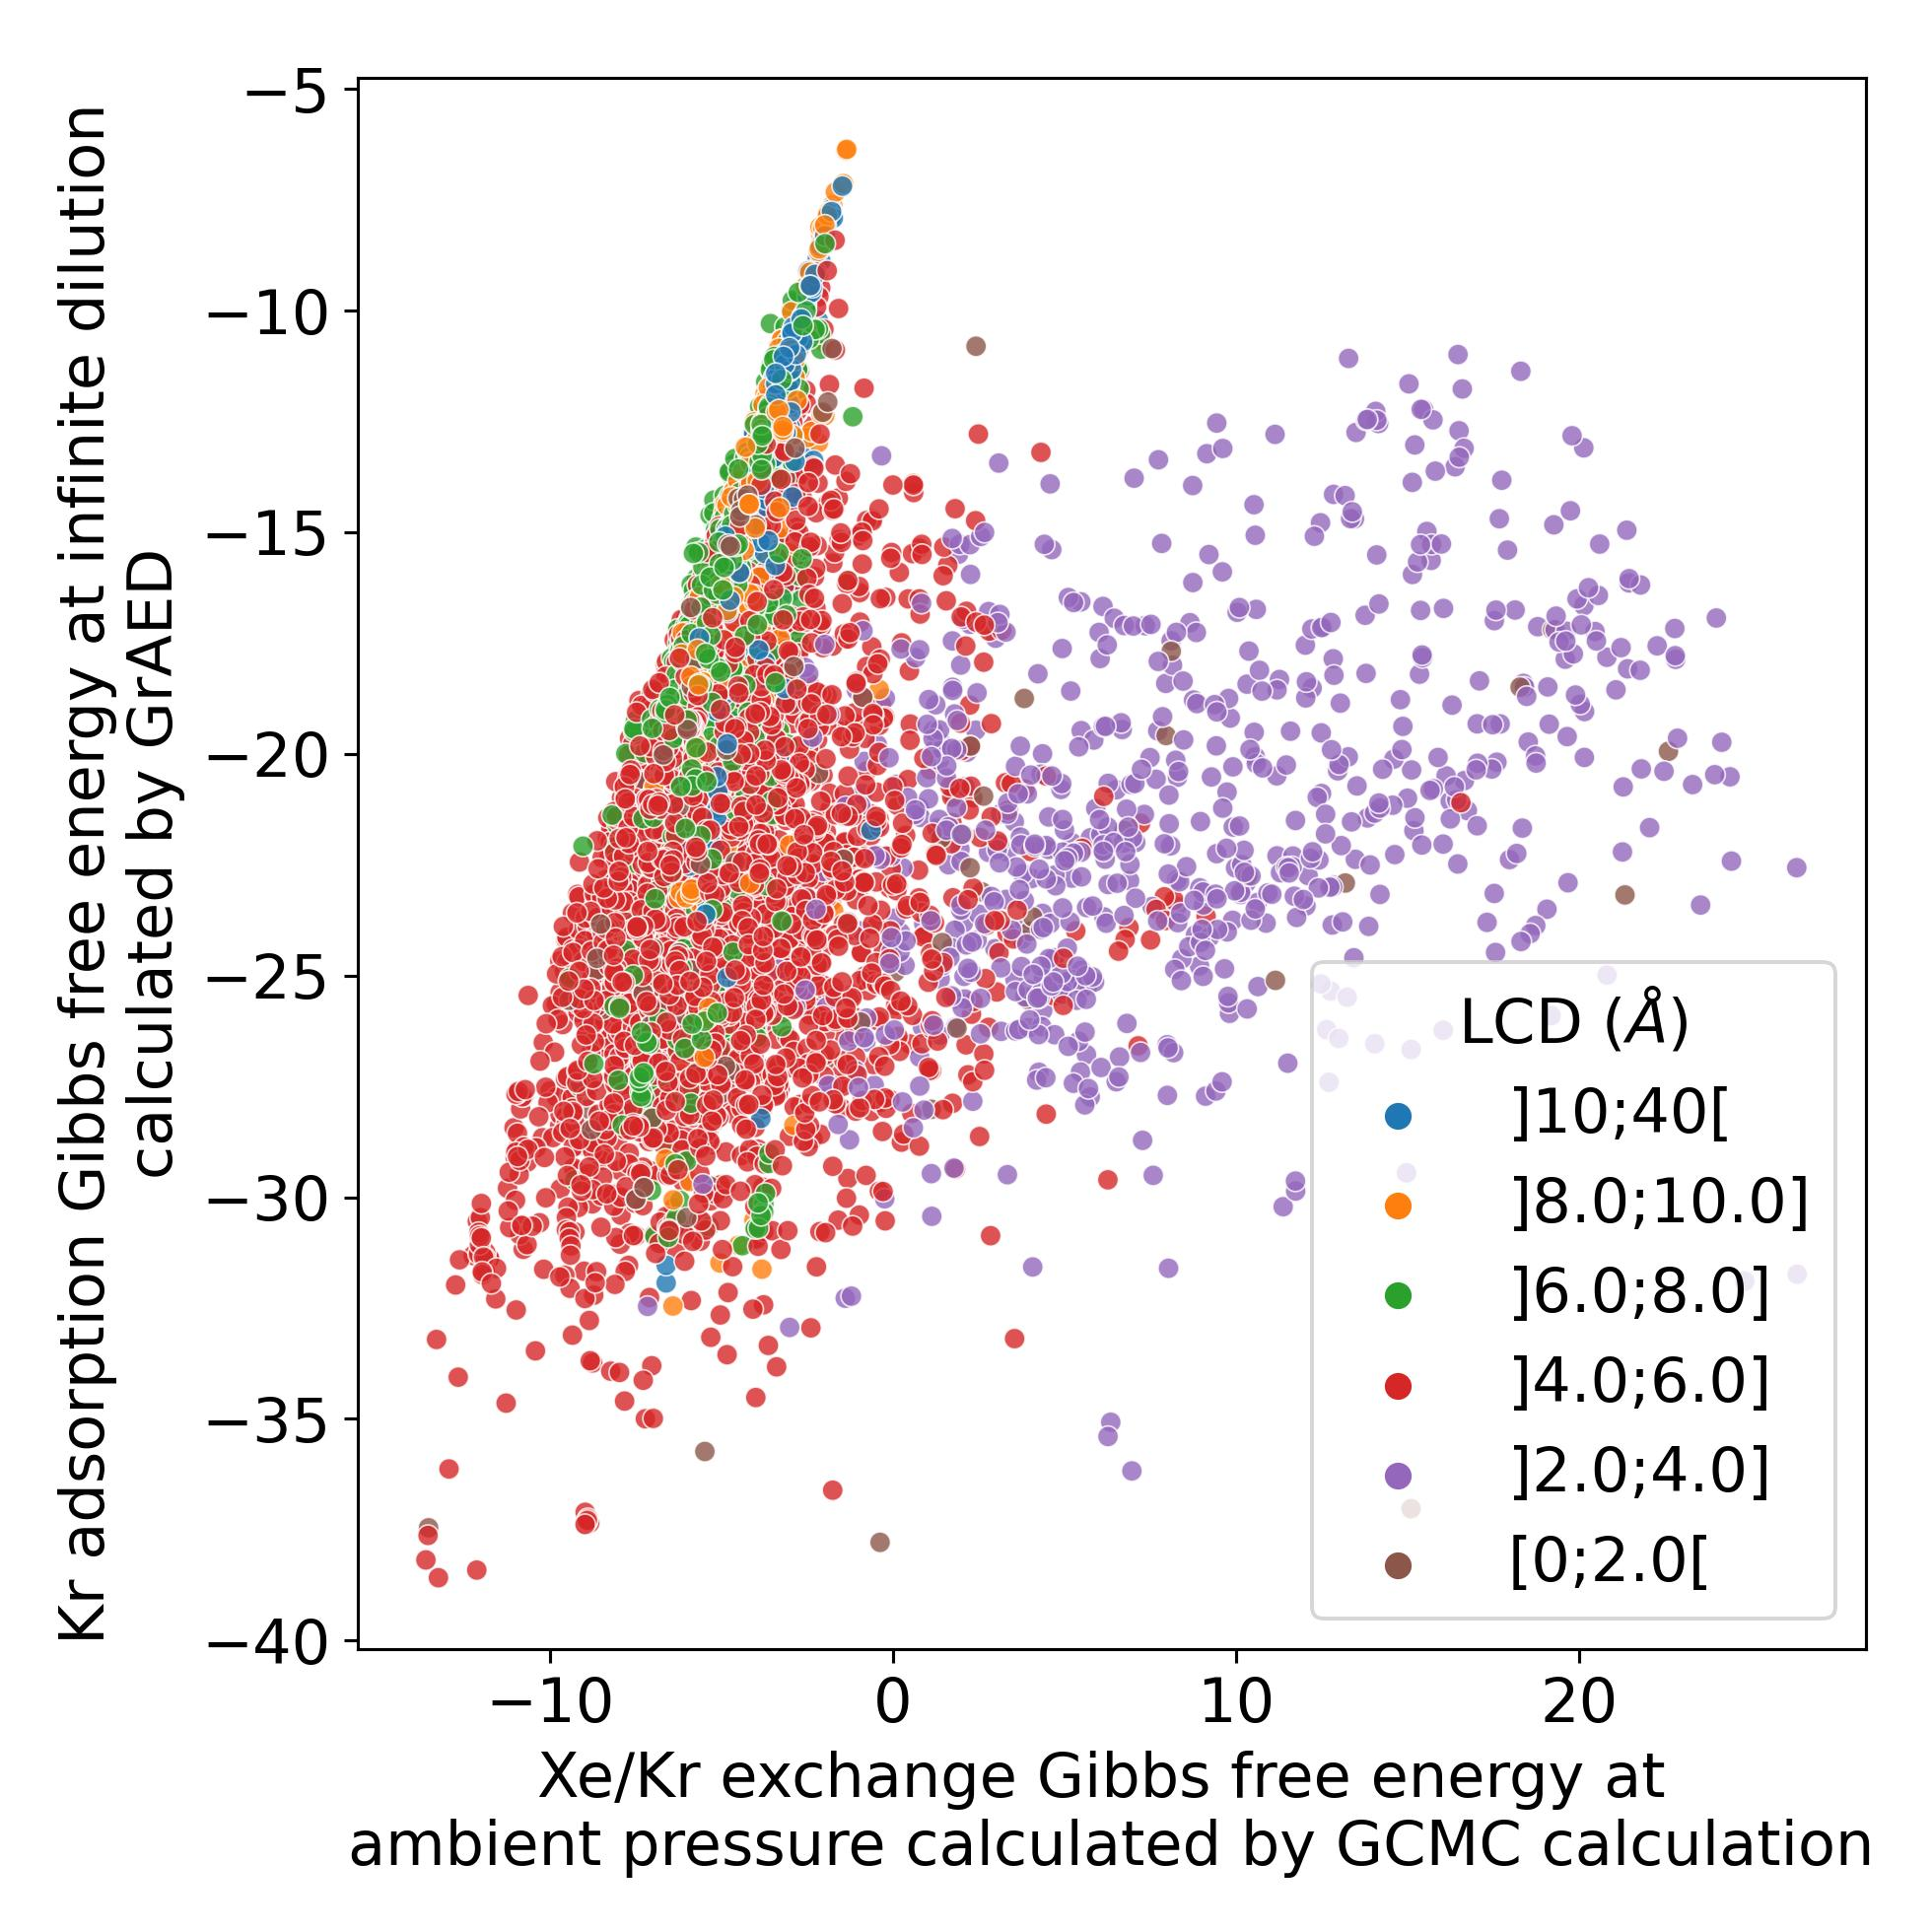
\includegraphics[width=0.45\textwidth]{figures/3-fastsim/G_2080_vs_H_Kr_grid_overview.jpg}
    \caption{Comparison of the ambient-pressure Xe/Kr exchange Gibbs free energy calculated by GCMC simulations of RASPA with 100,000 cycles and the low-pressure adsorption enthalpies of xenon (left) and krypton (right) in \si{\kilo\joule\per\mole} calculated by the GrAED algorithm (same parameters).}\label{fgr:grid_comp_enthalpy}
\end{figure}

The same statement on the importance of the adsorption attractiveness of xenon holds true when looking at the adsorption enthalpies from the Figure~\ref{fgr:grid_comp_enthalpy}. The correlation is very strong for the most selective materials; however, for less selective materials, the xenon adsorption enthalpy is not enough in predicting the exchange Gibbs free energy at ambient pressure. The solution would, of course, be to include the krypton into account first, the difference of both adsorption enthalpies give the exchange enthalpy which is  better quantity for comparison. The comparison to the krypton adsorption enthalpy alone is not sufficient either, the very loose correlation suggests that it is not the main explanatory factor in the separation process.

\begin{figure}[ht]
  \centering
    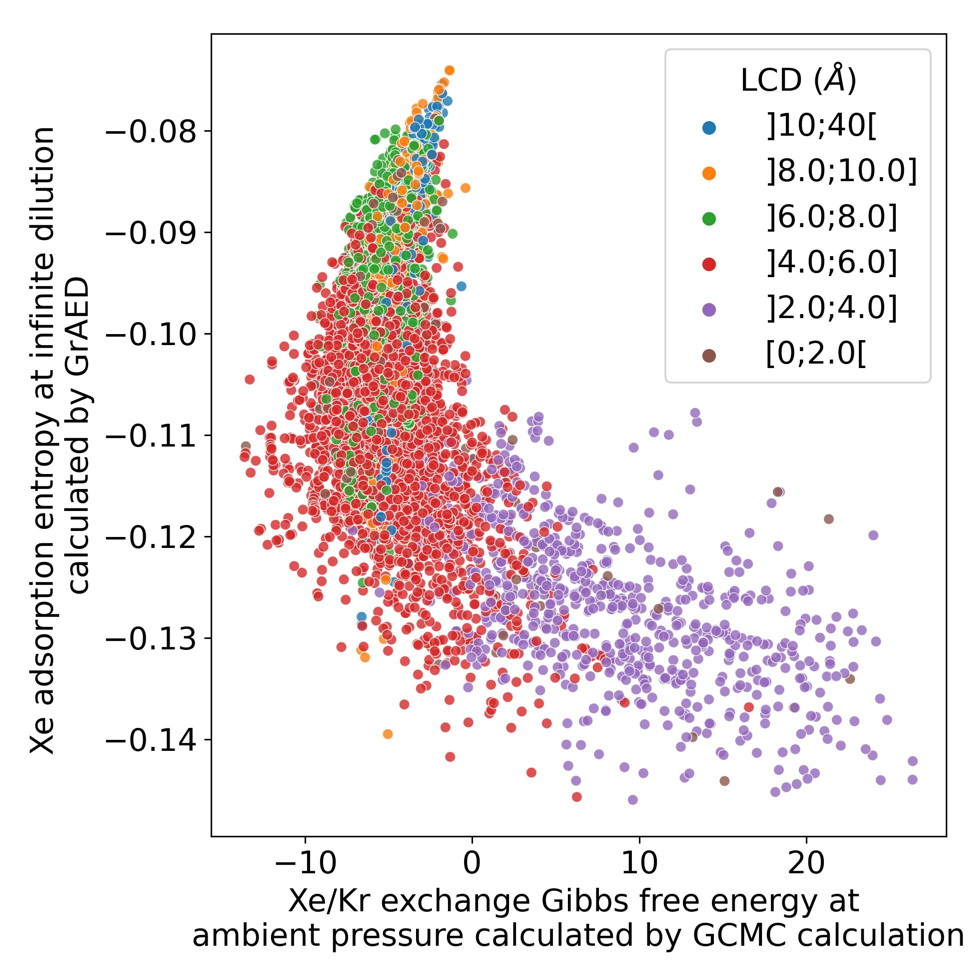
\includegraphics[width=0.45\textwidth]{figures/3-fastsim/G_2080_vs_S_Xe_grid_overview.jpg}
    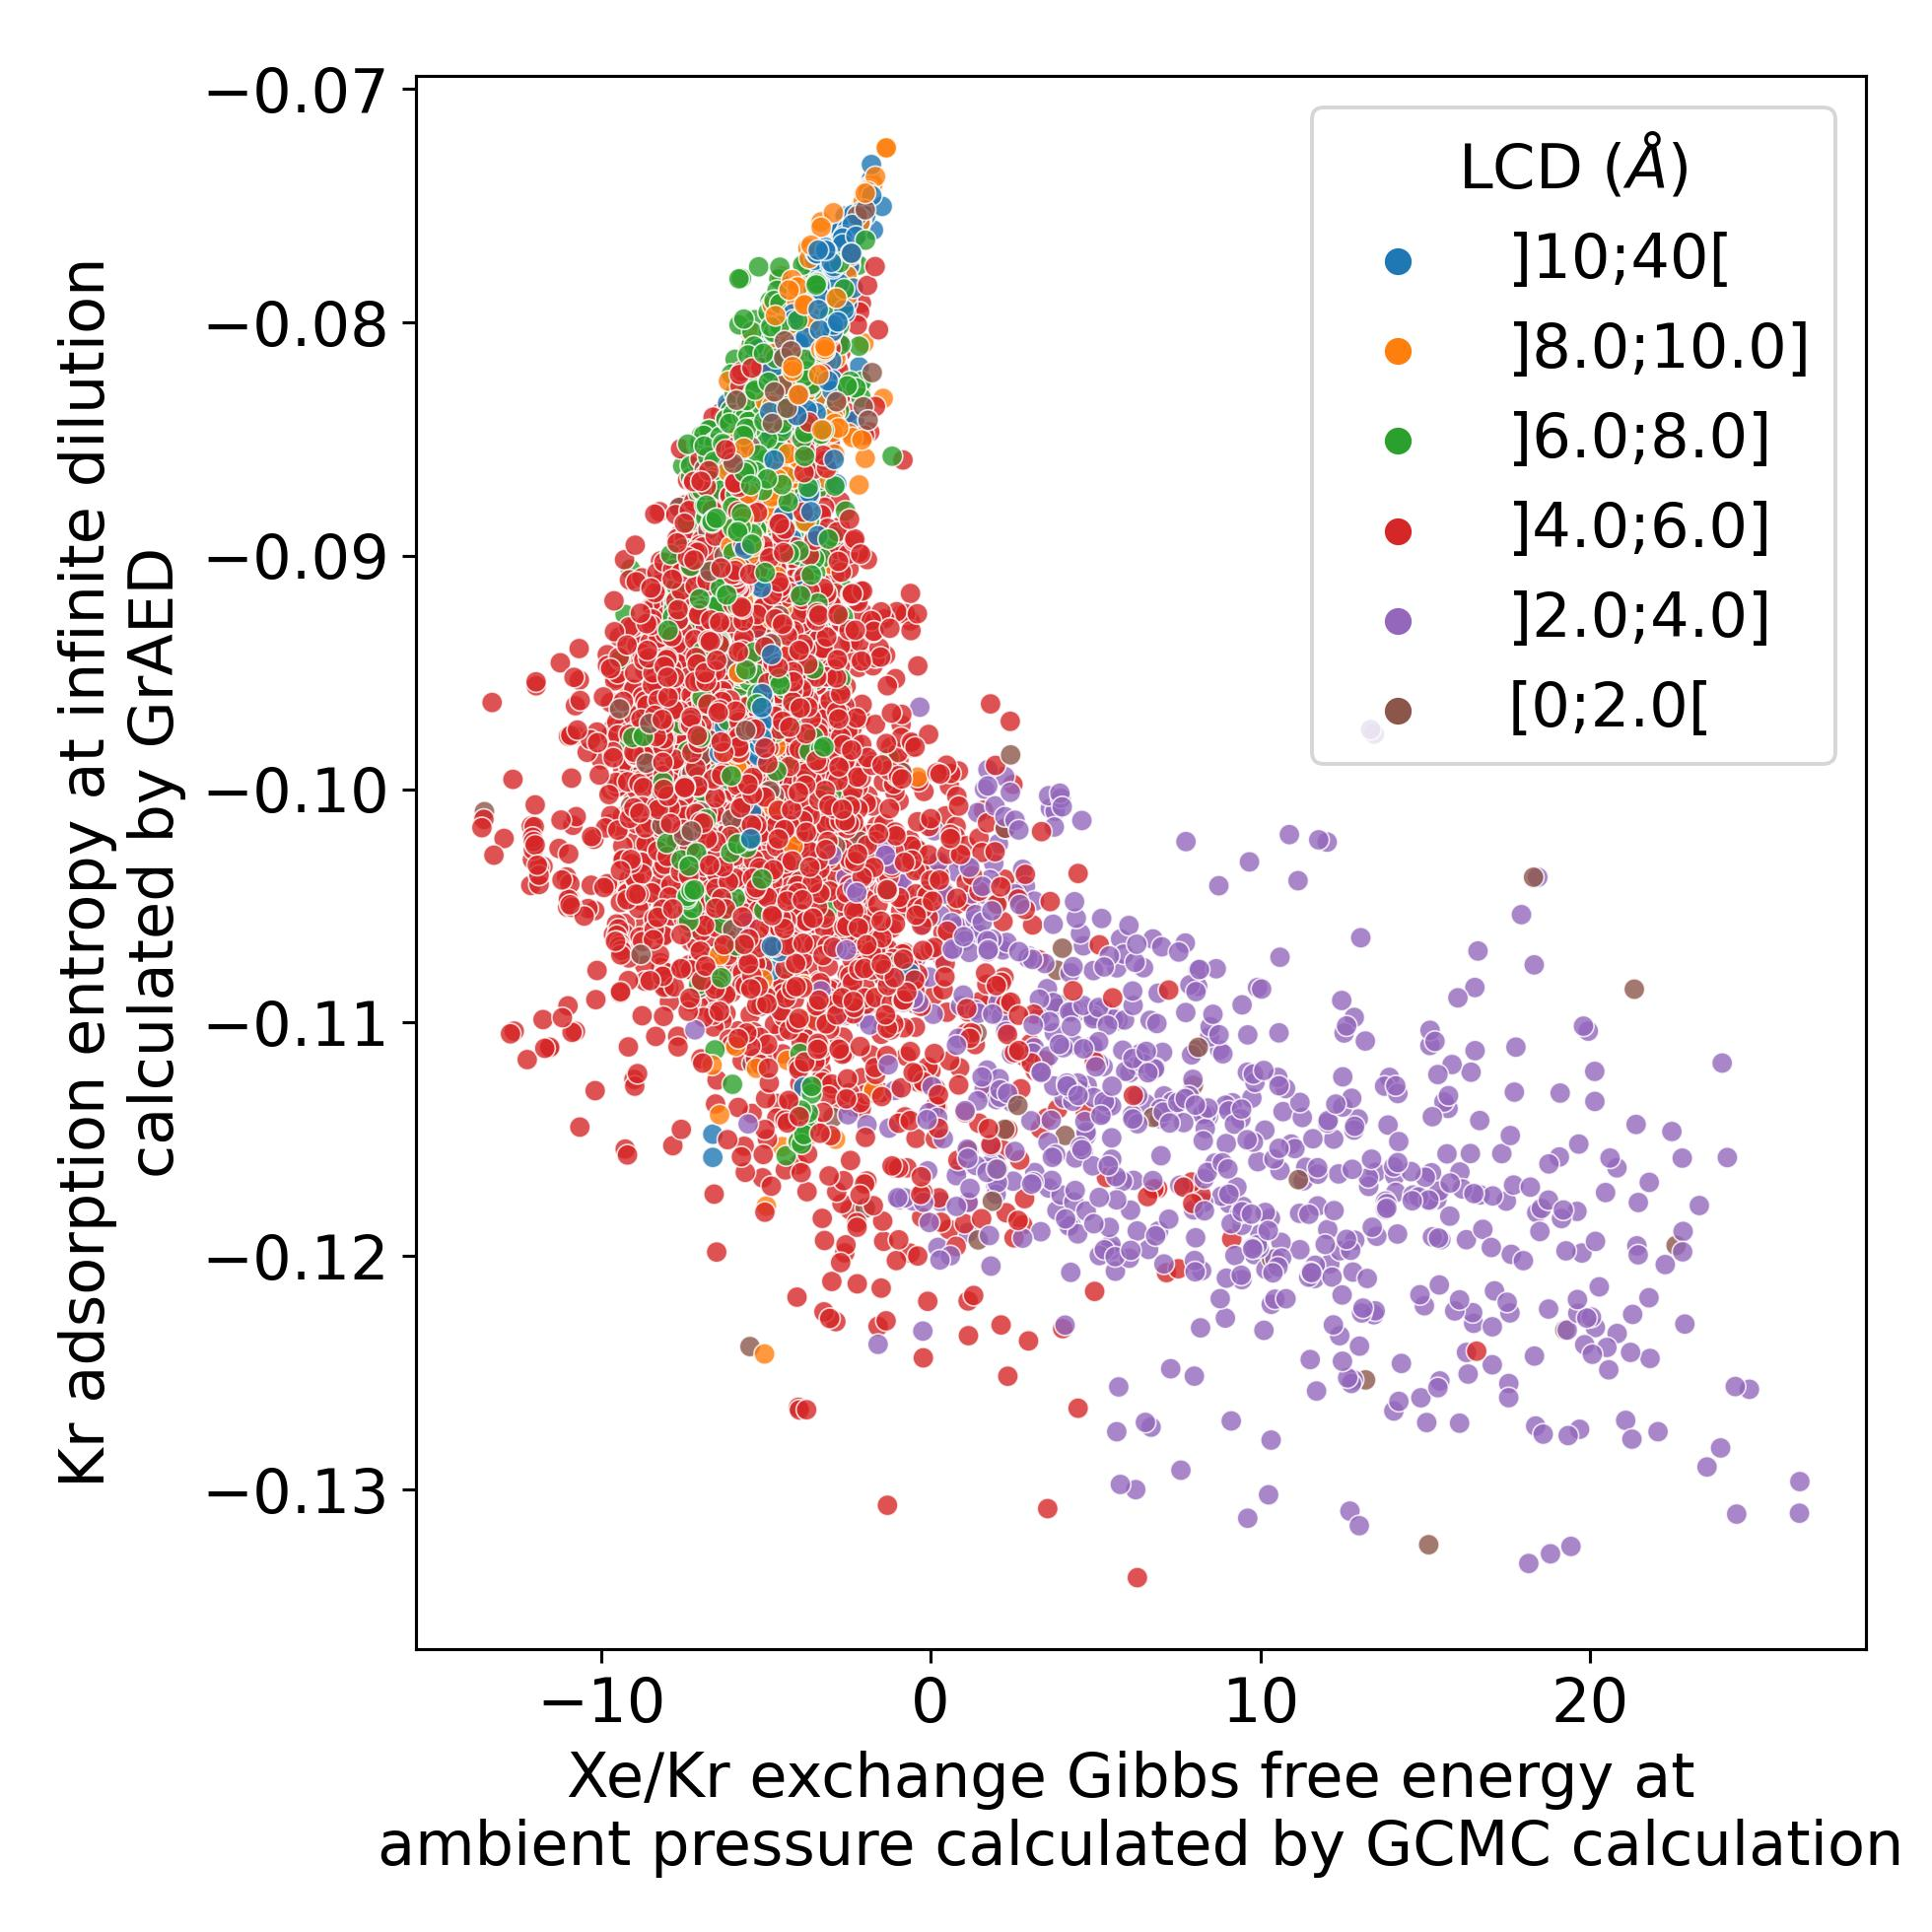
\includegraphics[width=0.45\textwidth]{figures/3-fastsim/G_2080_vs_S_Kr_grid_overview.jpg}
    \caption{Comparison of the ambient-pressure Xe/Kr exchange Gibbs free energy calculated by GCMC simulations of RASPA with 100,000 cycles and the low-pressure adsorption entropies of xenon (left) and krypton (right) in \si{\kilo\joule\per\mole\per\kelvin} calculated by the GrAED algorithm (same parameters).}\label{fgr:grid_comp_entropy}
\end{figure}

The entropy values can explain why the adsorption free energy of xenon is well correlated to the Xe/Kr exchange free energy at ambient pressure and the adsorption enthalpy of xenon is weakly correlated. The difference between enthalpy and free energy being the entropic term ($G=H-TS$), this entropic term has small influence on the correlation as we can see on the Figure~\ref{fgr:grid_comp_entropy}. The values of the entropy are rather stable (between $-0.15$ and $-0.11$~\si{\kilo\joule\per\mole\per\kelvin}), but for some structures with an ambient-pressure exchange free energy between $-10$ and $0$~\si{\kilo\joule\per\mole}, there is a swing in entropy values going from $-0.11$ and $-0.07$~\si{\kilo\joule\per\mole\per\kelvin} for structures with very similar values of enthalpy. This means difference between Gibbs free energy and enthalpy that could reach a span of $12$~\si{\kilo\joule\per\mole}, which explains the points that go off the diagonal in the left plot of the Figure~\ref{fgr:grid_comp_enthalpy}.

\begin{figure}[ht]
  \centering
    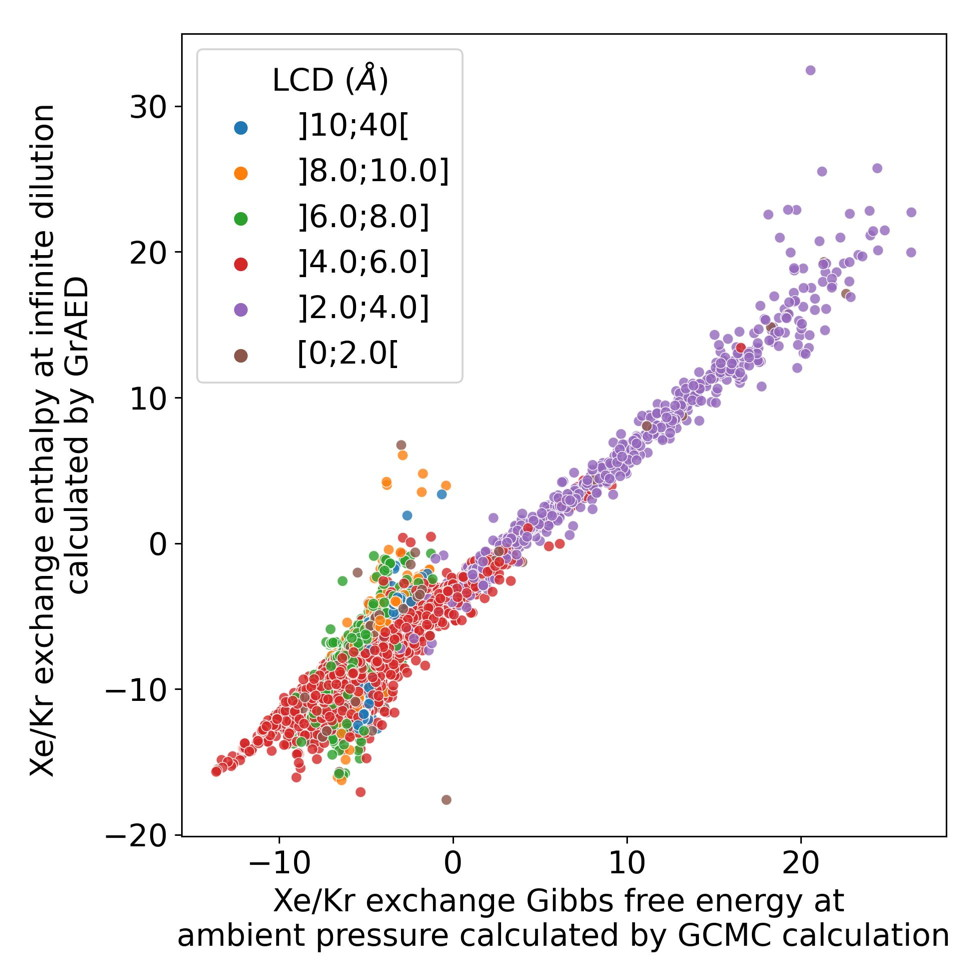
\includegraphics[width=0.45\textwidth]{figures/3-fastsim/G_2080_vs_H_grid_overview.jpg}
    \includegraphics[width=0.45\textwidth]{figures/3-fastsim/G_2080_vs_S_grid_overview.jpg}
    \caption{Comparison of the ambient-pressure Xe/Kr exchange Gibbs free energy calculated by GCMC simulations of RASPA with 100,000 cycles and the low-pressure exchange enthalpy (left, in \si{\kilo\joule\per\mole}) and entropy (right, in \si{\kilo\joule\per\mole\per\kelvin}) calculated by the GrAED algorithm (same parameters).}\label{fgr:grid_comp_exc}
\end{figure}

Now, if we go back to the exchange thermodynamic quantities that are more relevant to our context, we can see a good correlation between the exchange enthalpy at low pressure calculated with GrAED and the exchange Gibbs free energy at ambient pressure calculated by GCMC on Figure~\ref{fgr:grid_comp_exc}. Some discrepancies can be detected around $-10$ and $0$~\si{\kilo\joule\per\mole} of the ambient-pressure exchange free energy, which can also be explained using the exchange entropy that is stable $-0.01$~\si{\kilo\joule\per\mole\per\kelvin} and experiences a peak for structures near the previously mentioned range of ambient-pressure exchange free energy. The overall strong correlation can be explained using the previously identified enthalpic nature of the separation process of xenon from krypton (see chapter 2). And, the problematic range, where the correlation is weaker, also corresponds to the one associated with a selectivity drop in the Figure~\ref{fgr:G_900K}. These exchange thermodynamic quantities can help distinguish the materials to better model the drop phenomenon, a more quantitative approach will be developed in the next chapter.


\subsubsection{High-temperature quantities}

Although the previous quantities are valuable in modeling the adsorption at ambient pressure, they are still not enough, since they describe a state where the atoms adsorbe on the most attractive sites only. The ambient-pressure state is actually characterized by an adsorption on a more diverse set of sites and with an increasingly important role of the guest--host interaction, which are also the main factors that contribute to the difference in selectivity between both pressure conditions and identified in the previous chapter.

In this section, we introduce a descriptor that better describes the energy distribution in the ambient-pressure case by increasing the weight of the more energetic adsorption sites. To do so the easiest way was to increase the temperature in the Boltzmann averaging for both the Gibbs free energy and the enthalpy defined in equations~\ref{eq:ads_gibbs} and~\ref{eq:ads_enthalpy}. Many temperatures were tested, and the one that yielded the higher correlation coefficient when comparing the adsorption enthalpies (infinite dilution and ambient pressure) was chosen. 

A temperature of \SI{900}{\kelvin} was found to be the optimal temperature to describe an ambient-pressure adsorption enthalpy of xenon across the structures of CoRE MOF 2019, and gives a minimal error (RMSE) of \SI{1.76}{\kilo\joule\per\mole} instead of \SI{2.87}{\kilo\joule\per\mole} for the \SI{298}{\kelvin} case. This improvement impacts the exchange free energy metrics as well as the adsorption enthalpy associated with the separation of xenon from krypton. The exchange Gibbs free energy and the adsorption enthalpy of xenon at ambient pressure are better correlated to the equivalent values at lower pressure and higher temperature (\SI{900}{\kelvin}) than to the \SI{298}{\kelvin} case. These observations support the use of higher temperature averaging to describe the ambient-pressure selectivity.

This new type of descriptor is very interesting since it performs better around the high selectivity region, where the standard Boltzmann average at \SI{298}{\kelvin} loses its accuracy (see Figure~\ref{fgr:grid_ambient_selectivity}). As we can see in the Figures~\ref{fgr:H_900K} and~\ref{fgr:G_900K}, the averaging at higher temperature performs better on the most selective materials, while degrading the description of the less selective materials.

On the Figure~\ref{fgr:H_900K}, we can clearly see what an increase in the averaging temperature does: the low-temperature averaging gives a better description of the xenon adsorption enthalpy, the points are more centered around the $y=x$ axis, but the correlation is not perfect. We now also have a bigger uncertainty on the points that were initially very well predicted as badly performing materials. The high dispersion around the correlation is probably due to the guest--guest interactions that are not described in the high temperature averaging and plays a non-negligible role in the ambient pressure case.

\begin{figure}[ht]
\centering
  \includegraphics[width=0.45\linewidth]{figures/4-ml/SI_figure/Scatterplot_H1_H0.pdf}
  \includegraphics[width=0.45\linewidth]{figures/4-ml/SI_figure/Scatterplot_H1_H900K.pdf}
  \caption{Scatterplots of the low-pressure xenon adsorption enthalpy at \SI{298}{\kelvin} (left) and at \SI{900}{\kelvin} (right) calculated by the GrAED algorithm against the ambient-pressure xenon adsorption enthalpy at \SI{298}{\kelvin}. Using a higher temperature Boltzmann averaging, the correlation with the ambient-pressure case of interest is much higher, the R2 coefficient improves from $0.80$ to $0.92$ for instance. The RMSE also decreased from \SI{2.87}{\kilo\joule\per\mole} to \SI{1.76}{\kilo\joule\per\mole}. }\label{fgr:H_900K}
\end{figure}

On the Figure~\ref{fgr:G_900K}, we can see that this improvement in the adsorption enthalpy of xenon is not directly translated into the performance on the exchange Gibbs free energy. The correlation is better overall between the exchange free energy at \SI{298}{\kelvin} and infinite dilution and the one at ambient pressure (\SI{298}{\kelvin}). However, we can argue that the exchange free energy at \SI{900}{\kelvin} is, however, slightly better describing the materials that experience a selectivity drop as shown in Figure~\ref{fgr:grid_ambient_selectivity}. 

\begin{figure}[ht]
\centering
  \includegraphics[width=0.38\linewidth]{figures/3-fastsim/Scatterplot_G1_G0.pdf}
  \includegraphics[width=0.27\linewidth]{figures/3-fastsim/Scatterplot_G1_G900K.pdf}
  \includegraphics[width=0.23\linewidth]{figures/3-fastsim/Scatterplot_G1_G_Xe_900K.pdf}
  \caption{Comparison plot between the low-pressure exchange free energy at \SI{298}{\kelvin} (left) and \SI{900}{\kelvin} (right) calculated by the GrAED algorithm and the ambient-pressure exchange free energy at \SI{298}{\kelvin} calculated by Widom insertion. }\label{fgr:G_900K}
\end{figure}

This high-temperature averaging can be used to better model the selectivity of the selective materials that loses selectivity between low and ambient pressure. Without spoiling the incoming chapter on how we can exploit these descriptors to quantitatively predict the selectivity at ambient pressure, we can qualitatively see how a case disjunction between the problematic structures and the other and an exploitation of the values obtained can help us identify these problematic structures.

\subsubsection{Statistical characterization of the energy distributions}

To better quantify the change of selectivity, it could be interesting to give statistics on the distribution of interaction energies for xenon and krypton calculated by our grid algorithm. A statistical analysis can let us glimpse the complexity of the pore adsorption process at higher pressure by showing the diversity of the energy values and how they are distributed (the quantity of the higher energies in comparison to the lower ones, for example). The grid sampling we present here can use all the energy values from the sampled point to draw a histogram that can be used as an energy distribution and studied to retrieve interesting statistical information.

These statistics include the moments of different orders (up to 4) of the energy distribution, which informs on the adsorbate--adsorbent interaction energies in the nanopores at higher loading. The shape of the energy distribution can help assess quantitatively the change in selectivity. We can consider this as a way of compressing the whole energy distribution into a few statistical values, which is a standard method used in the field of data science to tackle distribution data. The energy distribution can be weighted uniformly or with the Boltzmann weights, both methods are explored here. The average of the Boltzmann weighted distribution is typically the definition of the adsorption enthalpy and it won't be tackled in this subsection.

\textbf{Boltzmann weighted distribution}

The Boltzmann weighted distribution consists in assigning a weight $\exp(-\beta E)$ according to the energy $E$ of each point sampled by the GrAED algorithm. By doing so, we put a much higher weight on the most negative values of the energy (the most favorable adsorption sites) than the others. The unfavorable adsorption sites can be considered negligible since the exponential scaling crushed the importance of these points in the Boltzmann weighted distribution. This distribution has already been used to calculate the adsorption enthalpy (first-order moment or average) and also indirectly the Henry constant (sum of the weights used in the normalization of the distribution). And in this section, we will focus on other statistical quantities that could be derived from the distribution and are not commonly used in describing the thermodynamics of the system.

\begin{figure}[ht]
  \centering
    \includegraphics[width=0.45\textwidth]{figures/3-fastsim/G_2080_vs_enthalpy_std_x_overview.jpg}
    \includegraphics[width=0.45\textwidth]{figures/3-fastsim/G_2080_vs_enthalpy_std_y_overview.jpg}
        \caption{Comparison of the ambient-pressure Xe/Kr exchange Gibbs free energy calculated by GCMC simulations of RASPA with 100,000 cycles and the standard deviations of the Boltzmann weighted energy distribution of xenon (left) and krypton (right) calculated by the GrAED algorithm at \SI{298}{\kelvin}.}\label{fgr:enthalpy_std}
\end{figure}

For instance, the standard deviation of the Boltzmann weighted energy distribution is one of the statistical quantities that could be interesting in evaluating the drop of selectivity. In the previous chapter, we identified the diversity of site attractiveness as one of the main factors that could explain the drop in selectivity. The standard deviation of the energies can therefore be useful characterization of the diversity of nature between the different adsorption sites. On the Figure~\ref{fgr:enthalpy_std}, this standard deviation is calculated for both xenon and krypton, and the higher variation of its values is concentrated in a range of values corresponding to the one we identified for the entropy change on one hand but more importantly to the range where the selectivity drop is observed on the Figure~\ref{fgr:G_900K} (between $-10$ and $0$~\si{\kilo\joule\per\mole}). Qualitatively, it is understandable that the standard deviation informs us on the pore diversity which could help characterizing the origins of the selectivity drop; and, the higher the diversity the higher probability of experiencing a selectivity drop. The challenge is then to quantify this probability through a model, a simple theoretical model would never be accurate enough, this is the reason we will be looking into machine learning models in the next chapter.

\begin{figure}[ht]
  \centering
    \includegraphics[width=0.45\textwidth]{figures/3-fastsim/G_2080_vs_enthalpy_skew_overview.jpg}
    \includegraphics[width=0.45\textwidth]{figures/3-fastsim/G_2080_vs_enthalpy_kurt_overview.jpg}
    \caption{Comparison of the ambient-pressure Xe/Kr exchange Gibbs free energy calculated by GCMC simulations of RASPA with 100,000 cycles and the skewness (left) and the kurtosis (right) of the Boltzmann weighted energy distribution of xenon calculated by the GrAED algorithm at \SI{298}{\kelvin}.}\label{fgr:enthalpy_skew_kurt}
\end{figure}

We introduced two other statistical quantities that could be interesting in describing the distribution: the skewness that characterizes the asymmetry of the distribution and the kurtosis that quantifies the ``tailedness'' (the number of values in the tail of the distribution). The first one is a standardized third moment while the second is a standardized fourth moment of the distribution. For a random variable $X$, whose mean value is $m$ and standard deviation $\sigma$ an n-th order moment $\text{M}_{n}(X)$ is defined as:
\begin{equation}
  \text{M}_n(X) = \mathbb{E}\left[\left(\dfrac{X-m}{\sigma}\right)^n\right]
\end{equation}
These quantities bring in another information on the distribution. For instance, if the distribution is skewed toward the most negative pore energies it would favor the adsorption at higher pressure, while the opposite would explain a bigger drop in selectivity. The overall shape of the distribution needs to be defined by more than the standard deviation and the mean value in order to capture the origins of the drop in selectivity. Ideally, it would be better to have the whole information on the distribution, but visually speaking, it would be far too complex to compare the structures according to this multidimensional descriptor and the statistical quantities compress in a way the complex data on the energy distribution.

The Figure~\ref{fgr:enthalpy_skew_kurt} further highlights the range of selectivity value we discussed across this section. The materials within this range can be sorted out using the different statistical quantities we introduced throughout this discussion. Depending on these skewness or kurtosis values it could be theoretically possible to identify a link with the selectivity drop previously identified, but without a model or a framework it is impossible to find the right relationship using our bare eyes.

% \todo{Negative skewness > bigger difference in selectivity value ?? Plot something skewness vs diff s1 s0}

\textbf{Uniformely weighted distribution}

To finish this overview on the thermodynamic/energetic descriptors we can deduce from the grid sampling we developed, we will study a more uniformly weighted energy distribution, and since the much higher energy values corresponding to the overlap with a framework atom does not interest us, these values are removed naturally by our sampling. Since a threshold value of $100$~\si{\kilo\joule\per\mole} has been used for the grid sampling here, the overlapping is defined very largely and for an energy below this value the energy point is taken into account. This distribution corresponds to the adsorbable sites (no overlap) that are weighted according to their sole occupancy of the void volume. 

We studied the mean value and the standard deviation of this distribution. For the mean value, we can observe a weak correlation with the exchange Gibbs energy at ambient pressure, but the correlation stops for the materials with larger pores and therefore a more diverse set of energy values, the mean value is lower since the void fraction is larger and the weight on the more negative values increase, but it does not mean that very attractive sites are present since there is no Boltzmann weight --- the exchange free energy is not continuing the trend and comes back to more positive values. We can note that the values are very high, this is because an energy threshold value of $100$~\si{\kilo\joule\per\mole} is used and a lot of points have values within zero and this threshold value, which shifts the mean toward these values. For this reason, we did not continue further than the standard deviation the statistical study of this distribution, and a better design of the distribution needs to be considered to focus more on the negative values --- it could be through lowering the threshold or by using a less skewing Boltzmann average (averaging at higher temperature for instance).

\begin{figure}[ht]
  \centering
    \includegraphics[width=0.45\textwidth]{figures/3-fastsim/G_2080_vs_mean_grid_x_overview.jpg}
    \includegraphics[width=0.45\textwidth]{figures/3-fastsim/G_2080_vs_std_grid_x_overview.jpg}
    \caption{Comparison of the ambient-pressure Xe/Kr exchange Gibbs free energy calculated by GCMC simulations of RASPA with 100,000 cycles and the mean values (left) and the standard deviation (right) of the uniformly weighted energy distribution of xenon calculated by the GrAED algorithm at \SI{298}{\kelvin}.}\label{fgr:energy_dist_mean_std}
\end{figure}

The standard deviation of this distribution has a lower value for materials with larger pores, see Figure~\ref{fgr:energy_dist_mean_std}. This could be explained by a high number of points near the average value of the energy (around $0$ and $10$~\si{\kilo\joule\per\mole}) according to the left plot of the figure. For the materials with a standard deviation between $20$ and $40$~\si{\kilo\joule\per\mole}, we can very confidently say that they have an exchange free energy that could not exceed $-8$~\si{\kilo\joule\per\mole}, which mean they are not in the top selective materials. The standard deviation presented here can help us identify materials that could be promising at low pressure but are not really promising in reality. 

To improve this approach, we can explore the use of a higher temperature Boltzmann average for the weights of the distribution, not necessarily using a temperature of \SI{900}{\kelvin}. We can also test out an average on a distribution with a lower energy threshold (zero or the mean kinetic energy of a gas $1.5k\e{B}T$). The idea being we want to characterize a higher energy state like the one happening at ambient pressure. And of course, higher orders of moments can also be tested to give a more complete picture of the distribution.

\vspace{2cm}

In this section, we tried to single out each of the thermodynamic descriptor we can derive from the grid sampling; the approach is limited by the visualization dimension limitation (bidimensional). Although we can see some examples, how it can help sorting the materials according to some properties that could at the end predict the selectivity (for instance, a given range of standard deviation of the uniformly weighted energy distribution can give a range of possible selectivity), it is still difficult to mix the different descriptors and to give a prediction. To achieve just this, many modern approaches use statistical learning to learn this relationship from a large enough set of structures with some computed properties, and this approach will be tested in the next chapter. Finally, every computation detail on the GrAED sampling technique is available online at \url{github.com/coudertlab/GrAED}.

\OnlyInSubfile{\printglobalbibliography}

\end{document}